% Annotated study edition of Office Hour One ("Groups") from
% Clay & Margalit, Office Hours with a Geometric Group Theorist (2017).
% Layout: original page image (left, unchanged) + annotation column (right).
% Build:  tectonic chapter1_annotated.tex
\documentclass[10pt]{article}
\usepackage{fontspec}
\setmainfont{Times New Roman}
\setsansfont{Helvetica Neue}
\usepackage{amsmath,amssymb,amsthm,mathtools}
\usepackage{graphicx}
\usepackage{xcolor}
\usepackage[absolute,overlay]{textpos}
\usepackage{tikz}
\usetikzlibrary{arrows.meta,calc,positioning,shapes.misc,decorations.markings}
\usepackage{tcolorbox}
\tcbuselibrary{skins}
\usepackage{enumitem}
\newcommand{\cmark}{\textcolor{why}{\ding{51}}}\newcommand{\xmark}{\textcolor{pit}{\ding{55}}}\usepackage{pifont}
\usepackage{array,booktabs}
\usepackage{geometry}
\geometry{paperwidth=11in,paperheight=8.5in,margin=0pt} % US Letter landscape
\pagestyle{empty}
\setlength{\parindent}{0pt}
\setlength{\parskip}{3pt}
\setlength{\TPHorizModule}{1pt}
\setlength{\TPVertModule}{1pt}
\linespread{1.08}

\definecolor{mkc}{RGB}{214,90,0}
\definecolor{why}{RGB}{30,120,60}
\definecolor{pit}{RGB}{180,30,40}
\definecolor{try}{RGB}{160,110,0}
\definecolor{ahead}{RGB}{90,50,160}
\definecolor{big}{RGB}{20,70,150}

\newcommand{\Z}{\mathbb{Z}}
\newcommand{\R}{\mathbb{R}}
\newcommand{\C}{\mathbb{C}}
\newcommand{\GL}{\mathrm{GL}}
\newcommand{\SL}{\mathrm{SL}}
\newcommand{\inv}{^{-1}}
\newcommand{\defterm}[1]{\textbf{\itshape #1}}

% ---------- marker on the book page ----------
\tikzset{marker/.style={circle,fill=mkc,text=white,font=\sffamily\bfseries\scriptsize,
  inner sep=0pt,minimum size=11pt}}
\newcommand{\mk}[3]{\node[marker] at (#2,#3) {#1};}
\newcommand{\hl}[4]{\fill[yellow,opacity=0.28] (#1,#2) rectangle ++(#3,#4);}
\newcommand{\num}[1]{\tikz[baseline=-3.5pt]\node[marker]{#1};}

% book page: #1 = png suffix (018 ...), #2 = book page number, #3 = marker code
\newcommand{\bookpage}[3]{%
  \begin{textblock*}{380pt}(24pt,20pt)\noindent\includegraphics[height=572pt]{pages/bk-#1.png}\end{textblock*}%
  \begin{textblock*}{380pt}(24pt,20pt)\noindent
    \begin{tikzpicture}[x=0.8602pt,y=-0.8602pt]
      \useasboundingbox (0,0) rectangle (442,665);
      #3
    \end{tikzpicture}
  \end{textblock*}%
  \begin{textblock*}{380pt}(24pt,594pt)\footnotesize\sffamily\color{gray}
    Office Hour 1, book page #2 \hfill annotated study edition\end{textblock*}%
}
% annotation column
\newcommand{\anncol}[1]{%
  \begin{textblock*}{350pt}(418pt,20pt)\small #1\end{textblock*}%
  \mbox{}\clearpage}
% full-width interlude page
\newcommand{\interlude}[2]{%
  \begin{textblock*}{744pt}(24pt,20pt)
    {\sffamily\bfseries\large\color{big} Interlude: #1}\par\vspace{4pt}
    \small #2\end{textblock*}\mbox{}\clearpage}

% ---------- annotation heading ----------
\newcommand{\A}[2]{\par\vspace{4pt}\noindent\num{#1}\ {\sffamily\bfseries #2}\par\nobreak\vspace{1pt}}

% ---------- boxes ----------
\newtcolorbox{why}{enhanced,colback=why!5,colframe=why,boxrule=0.5pt,arc=2pt,
  left=4pt,right=4pt,top=2pt,bottom=2pt,boxsep=1pt,fontupper=\small,
  title={\sffamily\bfseries Why?},fonttitle=\scriptsize,coltitle=white,colbacktitle=why,
  attach boxed title to top left={xshift=4pt,yshift=-2pt},boxed title style={size=small,arc=1pt,boxrule=0pt}}
\newtcolorbox{pitfall}{enhanced,colback=pit!5,colframe=pit,boxrule=0.5pt,arc=2pt,
  left=4pt,right=4pt,top=2pt,bottom=2pt,boxsep=1pt,fontupper=\small,
  title={\sffamily\bfseries Watch out},fonttitle=\scriptsize,coltitle=white,colbacktitle=pit,
  attach boxed title to top left={xshift=4pt,yshift=-2pt},boxed title style={size=small,arc=1pt,boxrule=0pt}}
\newtcolorbox{tryit}{enhanced,colback=try!6,colframe=try,boxrule=0.5pt,arc=2pt,
  left=4pt,right=4pt,top=2pt,bottom=2pt,boxsep=1pt,fontupper=\small,
  title={\sffamily\bfseries Try it},fonttitle=\scriptsize,coltitle=white,colbacktitle=try,
  attach boxed title to top left={xshift=4pt,yshift=-2pt},boxed title style={size=small,arc=1pt,boxrule=0pt}}
\newtcolorbox{lookahead}{enhanced,colback=ahead!5,colframe=ahead,boxrule=0.5pt,arc=2pt,
  left=4pt,right=4pt,top=2pt,bottom=2pt,boxsep=1pt,fontupper=\small,
  title={\sffamily\bfseries Looking ahead},fonttitle=\scriptsize,coltitle=white,colbacktitle=ahead,
  attach boxed title to top left={xshift=4pt,yshift=-2pt},boxed title style={size=small,arc=1pt,boxrule=0pt}}
\newtcolorbox{bigpic}{enhanced,colback=big!5,colframe=big,boxrule=0.5pt,arc=2pt,
  left=4pt,right=4pt,top=2pt,bottom=2pt,boxsep=1pt,fontupper=\small,
  title={\sffamily\bfseries Big picture},fonttitle=\scriptsize,coltitle=white,colbacktitle=big,
  attach boxed title to top left={xshift=4pt,yshift=-2pt},boxed title style={size=small,arc=1pt,boxrule=0pt}}
\newtcolorbox{prereq}{enhanced,colback=gray!8,colframe=gray!60!black,boxrule=0.5pt,arc=2pt,
  left=4pt,right=4pt,top=2pt,bottom=2pt,boxsep=1pt,fontupper=\small,
  title={\sffamily\bfseries Background you need},fonttitle=\scriptsize,coltitle=white,colbacktitle=gray!60!black,
  attach boxed title to top left={xshift=4pt,yshift=-2pt},boxed title style={size=small,arc=1pt,boxrule=0pt}}

% =====================================================================
%                              FIGURES
% =====================================================================
\newcommand{\figtriangle}{%
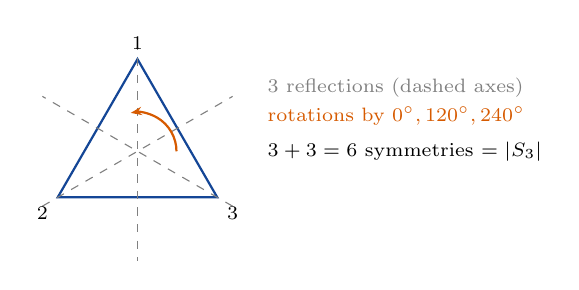
\begin{tikzpicture}[scale=0.9]
  \coordinate (A) at (90:1.3); \coordinate (B) at (210:1.3); \coordinate (C) at (330:1.3);
  \draw[thick,big] (A)--(B)--(C)--cycle;
  \foreach \ang in {90,210,330} \draw[dashed,gray] (\ang:1.55) -- (\ang+180:1.55);
  \draw[-{Stealth[length=4pt]},mkc,thick] (0.55,0) arc (0:100:0.55);
  \node[font=\scriptsize] at (A) [above] {1}; \node[font=\scriptsize] at (B) [below left] {2}; \node[font=\scriptsize] at (C) [below right] {3};
  \node[font=\scriptsize,text=gray,anchor=west] at (1.7,0.9) {3 reflections (dashed axes)};
  \node[font=\scriptsize,text=mkc,anchor=west] at (1.7,0.5) {rotations by $0^\circ,120^\circ,240^\circ$};
  \node[font=\scriptsize,anchor=west] at (1.7,0.0) {$3+3=6$ symmetries $=|S_3|$};
\end{tikzpicture}}

\newcommand{\figcube}[1]{%
\begin{tikzpicture}[scale=#1,line join=round]
  \coordinate (A) at (0,0); \coordinate (B) at (3,0); \coordinate (C) at (3,3); \coordinate (D) at (0,3);
  \coordinate (E) at (1.3,1.3); \coordinate (F) at (4.3,1.3); \coordinate (G) at (4.3,4.3); \coordinate (H) at (1.3,4.3);
  \draw[thick] (A)--(B)--(C)--(D)--cycle;
  \draw[thick] (B)--(F)--(G)--(C); \draw[thick] (D)--(H)--(G);
  \draw[thick,dashed,gray] (A)--(E)--(F); \draw[thick,dashed,gray] (E)--(H);
  \draw[very thick,red!80!black] (A)--(G);
  \draw[very thick,blue!70!black] (B)--(H);
  \draw[very thick,green!55!black] (C)--(E);
  \draw[very thick,orange!90!black] (D)--(F);
  \foreach \p/\l/\pos in {A/A/below left,B/B/below right,C/C/above right,D/D/above left,E/E/left,F/F/right,G/G/above right,H/H/above left}
    \node[font=\scriptsize,\pos] at (\p) {$\l$};
  \node[font=\scriptsize,red!80!black] at (2.6,2.9) {$d_1$};
  \node[font=\scriptsize,blue!70!black] at (1.7,1.55) {$d_2$};
  \node[font=\scriptsize,green!55!black] at (2.35,2.1) {$d_3$};
  \node[font=\scriptsize,orange!90!black] at (2.9,1.3) {$d_4$};
\end{tikzpicture}}

\newcommand{\figpent}{%
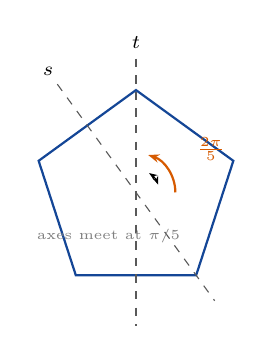
\begin{tikzpicture}[scale=1.0]
  \foreach \k in {0,...,4} \coordinate (P\k) at ({90+72*\k}:1.3);
  \draw[thick,big] (P0)--(P1)--(P2)--(P3)--(P4)--cycle;
  \draw[dashed,gray!70!black] (90:1.7)--(270:1.7);
  \draw[dashed,gray!70!black] (126:1.7)--(306:1.7);
  \node[font=\scriptsize] at (90:1.9) {$t$};
  \node[font=\scriptsize] at (126:1.9) {$s$};
  \draw[-{Stealth[length=4pt]},mkc,thick] (0.5,0) arc (0:72:0.5);
  \node[font=\scriptsize,mkc] at (0.95,0.55) {$\tfrac{2\pi}{5}$};
  \draw[{Stealth[length=3pt]}-{Stealth[length=3pt]},thin] (0.28,0.1) arc (20:56:0.3);
  \node[font=\tiny,gray] at (-0.35,-0.55) {axes meet at $\pi/5$};
\end{tikzpicture}}

\newcommand{\figcompose}{%
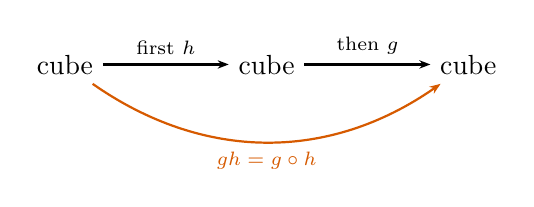
\begin{tikzpicture}[node distance=1.6cm,>={Stealth[length=4pt]}]
  \node (x) {cube};
  \node (y) [right=of x] {cube};
  \node (z) [right=of y] {cube};
  \draw[->,thick] (x) -- node[above,font=\scriptsize] {first $h$} (y);
  \draw[->,thick] (y) -- node[above,font=\scriptsize] {then $g$} (z);
  \draw[->,thick,mkc] (x) to[bend right=35] node[below,font=\scriptsize] {$gh=g\circ h$} (z);
\end{tikzpicture}}

\newcommand{\figbraid}{%
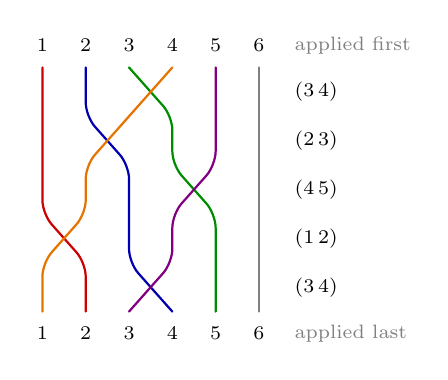
\begin{tikzpicture}[x=0.55cm,y=0.62cm,line cap=round]
  \foreach \i in {1,...,6} {\node[font=\scriptsize] at (\i,0.45) {\i}; \node[font=\scriptsize] at (\i,-5.45) {\i};}
  \draw[thick,red!80!black,rounded corners=5pt] (1,0)--(1,-1)--(1,-2)--(1,-3)--(2,-4)--(2,-5);
  \draw[thick,blue!70!black,rounded corners=5pt] (2,0)--(2,-1)--(3,-2)--(3,-3)--(3,-4)--(4,-5);
  \draw[thick,green!55!black,rounded corners=5pt] (3,0)--(4,-1)--(4,-2)--(5,-3)--(5,-4)--(5,-5);
  \draw[thick,orange!90!black,rounded corners=5pt] (4,0)--(3,-1)--(2,-2)--(2,-3)--(1,-4)--(1,-5);
  \draw[thick,violet,rounded corners=5pt] (5,0)--(5,-1)--(5,-2)--(4,-3)--(4,-4)--(3,-5);
  \draw[thick,gray] (6,0)--(6,-5);
  \foreach \y/\l in {0.5/(3\,4), 1.5/(2\,3), 2.5/(4\,5), 3.5/(1\,2), 4.5/(3\,4)}
    \node[font=\scriptsize,anchor=west] at (6.6,-\y) {$\l$};
  \node[font=\scriptsize,anchor=west,gray] at (6.6,0.45) {applied first};
  \node[font=\scriptsize,anchor=west,gray] at (6.6,-5.45) {applied last};
\end{tikzpicture}}

\newcommand{\figstack}{%
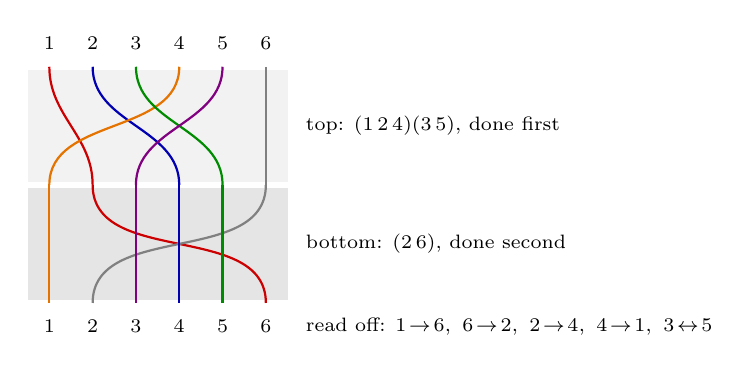
\begin{tikzpicture}[x=0.55cm,y=0.75cm]
  \foreach \i in {1,...,6} {\node[font=\scriptsize] at (\i,0.4) {\i}; \node[font=\scriptsize] at (\i,-4.4) {\i};}
  \fill[gray!10] (0.5,-0.05) rectangle (6.5,-1.95);
  \fill[gray!20] (0.5,-2.05) rectangle (6.5,-3.95);
  % top block: (1 2 4)(3 5): i -> sigma(i)
  \foreach \a/\b/\c in {1/2/red!80!black, 2/4/blue!70!black, 4/1/orange!90!black, 3/5/green!55!black, 5/3/violet, 6/6/gray}
    \draw[thick,\c] (\a,0) to[out=-90,in=90] (\b,-2);
  % bottom block: (2 6)
  \foreach \a/\b/\c in {2/6/red!80!black, 6/2/gray, 1/1/orange!90!black, 3/3/violet, 4/4/blue!70!black, 5/5/green!55!black}
    \draw[thick,\c] (\a,-2) to[out=-90,in=90] (\b,-4);
  \node[font=\scriptsize,anchor=west] at (6.7,-1) {top: $(1\,2\,4)(3\,5)$, done first};
  \node[font=\scriptsize,anchor=west] at (6.7,-3) {bottom: $(2\,6)$, done second};
  \node[font=\scriptsize,anchor=west] at (6.7,-4.4) {read off: $1\!\to\!6,\ 6\!\to\!2,\ 2\!\to\!4,\ 4\!\to\!1,\ 3\!\leftrightarrow\!5$};
\end{tikzpicture}}

\newcommand{\figclock}{%
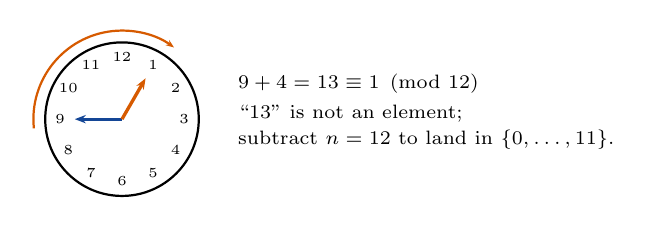
\begin{tikzpicture}[scale=0.75]
  \draw[thick] (0,0) circle (1.3);
  \foreach \h in {1,...,12} \node[font=\tiny] at ({90-30*\h}:1.05) {\h};
  \draw[-{Stealth[length=4pt]},very thick,big] (0,0) -- ({90-30*9}:0.8);
  \draw[-{Stealth[length=4pt]},very thick,mkc] (0,0) -- ({90-30*1}:0.8);
  \draw[-{Stealth[length=3pt]},mkc,thick] ({90-30*9+6}:1.5) arc ({90-30*9+6}:{90-30*13-6}:1.5);
  \node[font=\scriptsize,anchor=west] at (1.8,0.6) {$9+4=13\equiv 1 \pmod{12}$};
  \node[font=\scriptsize,anchor=west] at (1.8,0.1) {``$13$'' is not an element;};
  \node[font=\scriptsize,anchor=west] at (1.8,-0.35) {subtract $n=12$ to land in $\{0,\dots,11\}$.};
\end{tikzpicture}}

\newcommand{\figarrowgon}{%
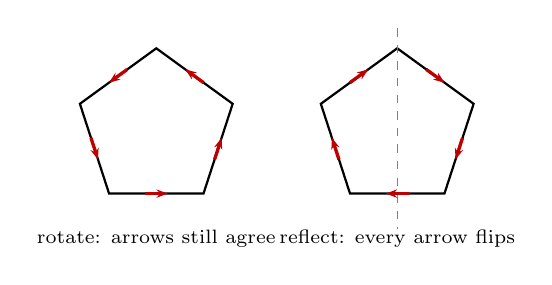
\begin{tikzpicture}[scale=0.85]
  \begin{scope}
    \foreach \k in {0,...,4} \coordinate (P\k) at ({90+72*\k}:1.2);
    \draw[thick] (P0)--(P1)--(P2)--(P3)--(P4)--cycle;
    \foreach \k in {0,...,4} {\pgfmathtruncatemacro{\nk}{mod(\k+1,5)}
      \draw[-{Stealth[length=4pt]},very thick,red!75!black] ($(P\k)!0.38!(P\nk)$)--($(P\k)!0.62!(P\nk)$);}
    \node[font=\scriptsize] at (0,-1.65) {rotate: arrows still agree};
  \end{scope}
  \begin{scope}[xshift=3.6cm]
    \foreach \k in {0,...,4} \coordinate (Q\k) at ({90-72*\k}:1.2);
    \draw[thick] (Q0)--(Q1)--(Q2)--(Q3)--(Q4)--cycle;
    \draw[dashed,gray] (0,1.5)--(0,-1.5);
    \foreach \k in {0,...,4} {\pgfmathtruncatemacro{\nk}{mod(\k+1,5)}
      \draw[-{Stealth[length=4pt]},very thick,red!75!black] ($(Q\k)!0.38!(Q\nk)$)--($(Q\k)!0.62!(Q\nk)$);}
    \node[font=\scriptsize] at (0,-1.65) {reflect: every arrow flips};
  \end{scope}
\end{tikzpicture}}

\newcommand{\figline}{%
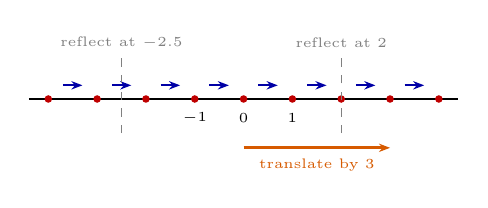
\begin{tikzpicture}[scale=0.62]
  \draw[thick] (-4.4,0)--(4.4,0);
  \foreach \x in {-4,...,4} \fill[red!75!black] (\x,0) circle (2.2pt);
  \foreach \x in {-4,...,3} \draw[-{Stealth[length=4pt]},thick,blue!65!black] (\x+0.3,0.28)--(\x+0.7,0.28);
  \node[font=\tiny] at (0,-0.4) {0}; \node[font=\tiny] at (1,-0.4) {1}; \node[font=\tiny] at (-1,-0.4) {$-1$};
  \draw[dashed,gray] (2,-0.7)--(2,0.9); \node[font=\tiny,gray] at (2,1.15) {reflect at 2};
  \draw[dashed,gray] (-2.5,-0.7)--(-2.5,0.9); \node[font=\tiny,gray] at (-2.5,1.15) {reflect at $-2.5$};
  \draw[-{Stealth[length=4pt]},very thick,mkc] (0,-1.0) -- (3,-1.0); \node[font=\tiny,mkc] at (1.5,-1.35) {translate by $3$};
\end{tikzpicture}}

\newcommand{\figlattice}{%
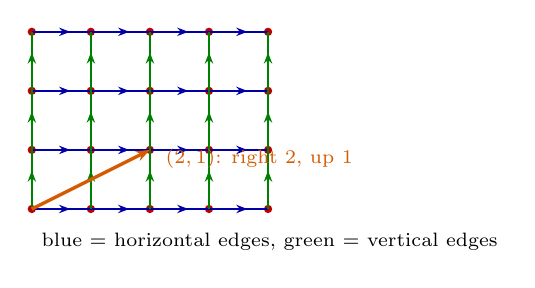
\begin{tikzpicture}[scale=0.75]
  \foreach \x in {0,...,4} \foreach \y in {0,...,3} \fill[red!75!black] (\x,\y) circle (2pt);
  \foreach \y in {0,...,3} \foreach \x in {0,...,3} {
    \draw[blue!65!black,thick] (\x,\y)--(\x+1,\y);
    \draw[-{Stealth[length=4pt]},blue!65!black,thick] (\x+0.35,\y)--(\x+0.65,\y);}
  \foreach \x in {0,...,4} \foreach \y in {0,...,2} {
    \draw[green!50!black,thick] (\x,\y)--(\x,\y+1);
    \draw[-{Stealth[length=4pt]},green!50!black,thick] (\x,\y+0.35)--(\x,\y+0.65);}
  \draw[-{Stealth[length=5pt]},very thick,mkc] (0,0)--(2,1);
  \node[font=\scriptsize,mkc,anchor=west] at (2.1,0.85) {$(2,1)$: right 2, up 1};
  \node[font=\scriptsize,anchor=north west] at (0,-0.25) {blue = horizontal edges, green = vertical edges};
\end{tikzpicture}}

\newcommand{\figreduce}{%
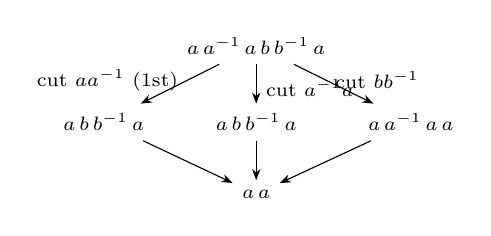
\begin{tikzpicture}[node distance=5mm and 3mm,>={Stealth[length=4pt]},every node/.style={font=\scriptsize}]
  \node (w) {$a\,a\inv\,a\,b\,b\inv\,a$};
  \node (l) [below left=of w] {$a\,b\,b\inv\,a$};
  \node (m) [below=of w] {$a\,b\,b\inv\,a$};
  \node (r) [below right=of w] {$a\,a\inv\,a\,a$};
  \node (e) [below=of m] {$a\,a$};
  \draw[->] (w) -- node[left,pos=0.4] {cut $a a\inv$ (1st)} (l);
  \draw[->] (w) -- node[right,pos=0.6] {cut $a\inv a$} (m);
  \draw[->] (w) -- node[right,pos=0.4] {cut $b b\inv$} (r);
  \draw[->] (l) -- (e); \draw[->] (m) -- (e); \draw[->] (r) -- (e);
\end{tikzpicture}}

\newcommand{\figtree}{%
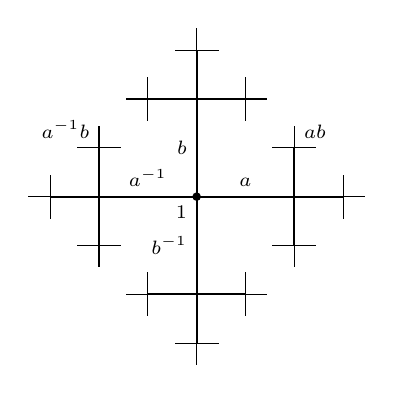
\begin{tikzpicture}[scale=0.62]
  \foreach \d/\o in {0/180,90/270,180/0,270/90} {
    \draw[thick] (0,0) -- (\d:2);
    \foreach \e in {0,90,180,270} {
      \ifnum\e=\o\relax\else
        \draw[thick] (\d:2) -- ($(\d:2)+(\e:1)$);
        \pgfmathtruncatemacro{\eo}{mod(\e+180,360)}
        \foreach \f in {0,90,180,270} {
          \ifnum\f=\eo\relax\else
            \draw[thin] ($(\d:2)+(\e:1)$) -- ($(\d:2)+(\e:1)+(\f:0.45)$);
          \fi }
      \fi } }
  \fill (0,0) circle (2.5pt);
  \node[font=\scriptsize,above] at (1,0) {$a$};
  \node[font=\scriptsize,left] at (0,1) {$b$};
  \node[font=\scriptsize,above] at (-1,0) {$a\inv$};
  \node[font=\scriptsize,left] at (0,-1) {$b\inv$};
  \node[font=\scriptsize,below left] at (0,0) {$1$};
  \node[font=\scriptsize,above right] at (2,1) {$ab$};
  \node[font=\scriptsize,above left] at (-2,1) {$a\inv b$};
\end{tikzpicture}}

\newcommand{\fighom}{%
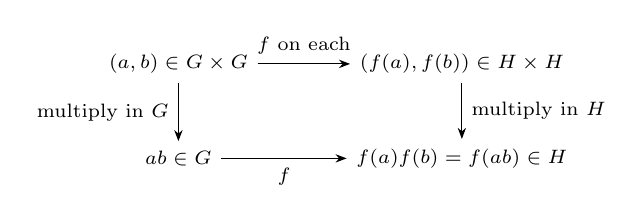
\begin{tikzpicture}[>={Stealth[length=4pt]},every node/.style={font=\scriptsize}]
  \node (a) at (0,1.2) {$(a,b)\in G\times G$};
  \node (b) at (3.6,1.2) {$(f(a),f(b))\in H\times H$};
  \node (c) at (0,0) {$ab\in G$};
  \node (d) at (3.6,0) {$f(a)f(b)=f(ab)\in H$};
  \draw[->] (a) -- node[above] {$f$ on each} (b);
  \draw[->] (a) -- node[left] {multiply in $G$} (c);
  \draw[->] (b) -- node[right] {multiply in $H$} (d);
  \draw[->] (c) -- node[below] {$f$} (d);
\end{tikzpicture}}

\newcommand{\figwrap}{%
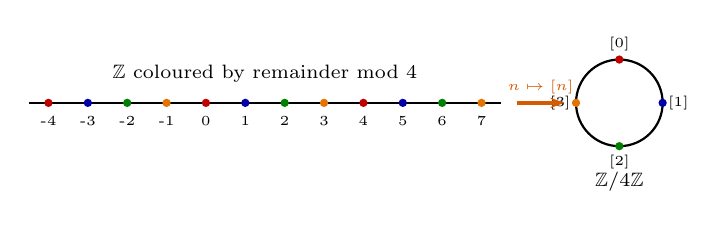
\begin{tikzpicture}[scale=0.5]
  \draw[thick] (-4.5,0)--(7.5,0);
  \foreach \x in {-4,...,7} {\pgfmathtruncatemacro{\r}{mod(\x+8,4)}
    \ifnum\r=0 \fill[red!75!black] (\x,0) circle (3pt);\fi
    \ifnum\r=1 \fill[blue!65!black] (\x,0) circle (3pt);\fi
    \ifnum\r=2 \fill[green!50!black] (\x,0) circle (3pt);\fi
    \ifnum\r=3 \fill[orange!90!black] (\x,0) circle (3pt);\fi
    \node[font=\tiny] at (\x,-0.45) {\x};}
  \node[font=\scriptsize] at (1.5,0.75) {$\Z$ coloured by remainder mod 4};
  \begin{scope}[xshift=10.5cm]
    \draw[thick] (0,0) circle (1.1);
    \fill[red!75!black] (90:1.1) circle (3pt); \node[font=\tiny] at (90:1.5) {$[0]$};
    \fill[blue!65!black] (0:1.1) circle (3pt); \node[font=\tiny] at (0:1.5) {$[1]$};
    \fill[green!50!black] (270:1.1) circle (3pt); \node[font=\tiny] at (270:1.5) {$[2]$};
    \fill[orange!90!black] (180:1.1) circle (3pt); \node[font=\tiny] at (180:1.5) {$[3]$};
    \node[font=\scriptsize] at (0,-2.0) {$\Z/4\Z$};
  \end{scope}
  \draw[-{Stealth[length=5pt]},very thick,mkc] (7.9,0) -- (9.1,0); \node[font=\tiny,mkc] at (8.5,0.4) {$n\mapsto[n]$};
\end{tikzpicture}}

\newcommand{\figiso}{%
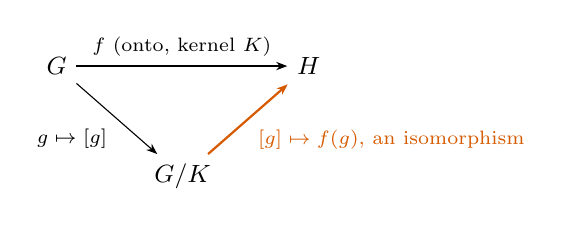
\begin{tikzpicture}[>={Stealth[length=4pt]},every node/.style={font=\small}]
  \node (G) at (0,1.4) {$G$};
  \node (H) at (3.2,1.4) {$H$};
  \node (Q) at (1.6,0) {$G/K$};
  \draw[->] (G) -- node[above,font=\scriptsize] {$f$ (onto, kernel $K$)} (H);
  \draw[->] (G) -- node[below left,font=\scriptsize] {$g\mapsto[g]$} (Q);
  \draw[->,mkc,thick] (Q) -- node[below right,font=\scriptsize] {$[g]\mapsto f(g)$, an isomorphism} (H);
\end{tikzpicture}}

\newcommand{\figpres}{%
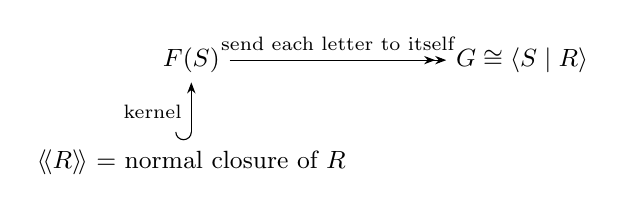
\begin{tikzpicture}[>={Stealth[length=4pt]},every node/.style={font=\small}]
  \node (F) at (0,0) {$F(S)$};
  \node (G) at (4.2,0) {$G\cong\langle S\mid R\rangle$};
  \node (N) at (0,-1.3) {$\langle\!\langle R\rangle\!\rangle$ = normal closure of $R$};
  \draw[-{Stealth[length=4pt]Stealth[length=4pt]}] (F) -- node[above,font=\scriptsize] {send each letter to itself} (G);
  \draw[{Hooks[right,length=3pt]}-{Stealth[length=4pt]}] (N) -- node[left,font=\scriptsize] {kernel} (F);
\end{tikzpicture}}

\newcommand{\figmap}{%
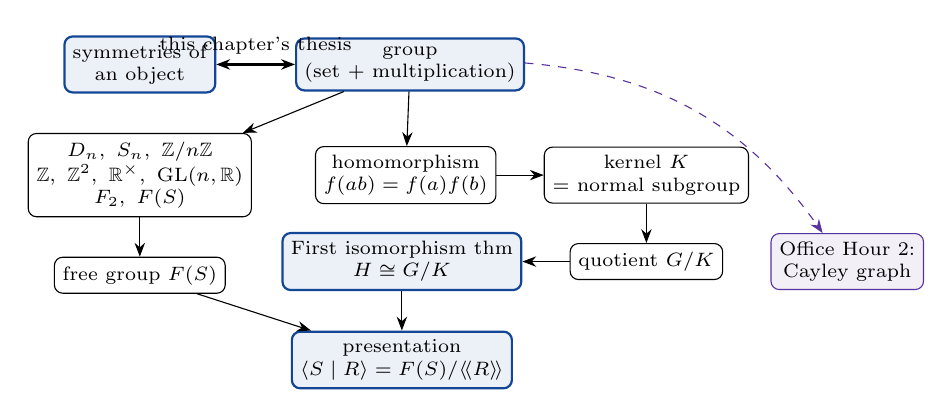
\begin{tikzpicture}[>={Stealth[length=5pt]},node distance=5mm and 6mm,
  box/.style={draw,rounded corners=3pt,align=center,font=\scriptsize,inner sep=3pt,fill=white},
  key/.style={box,fill=big!8,draw=big,thick}]
  \node[key] (sym) {symmetries of\\an object};
  \node[key,right=10mm of sym] (grp) {group\\(set + multiplication)};
  \node[box,below=of sym] (ex) {$D_n,\ S_n,\ \Z/n\Z$\\$\Z,\ \Z^2,\ \R^\times,\ \GL(n,\R)$\\$F_2,\ F(S)$};
  \node[box,right=8mm of ex] (hom) {homomorphism\\$f(ab)=f(a)f(b)$};
  \node[box,right=of hom] (ker) {kernel $K$\\= normal subgroup};
  \node[box,below=of ker] (quo) {quotient $G/K$};
  \node[key,left=of quo] (iso) {First isomorphism thm\\$H\cong G/K$};
  \node[box,below=of ex] (free) {free group $F(S)$};
  \node[key,below=of iso] (pres) {presentation\\$\langle S\mid R\rangle = F(S)/\langle\!\langle R\rangle\!\rangle$};
  \node[box,right=of quo,fill=ahead!8,draw=ahead] (cay) {Office Hour 2:\\Cayley graph};
  \draw[<->,thick] (sym) -- node[above,font=\scriptsize] {this chapter's thesis} (grp);
  \draw[->] (grp) -- (ex); \draw[->] (grp) -- (hom); \draw[->] (hom) -- (ker); \draw[->] (ker) -- (quo);
  \draw[->] (quo) -- (iso); \draw[->] (ex) -- (free); \draw[->] (free) -- (pres); \draw[->] (iso) -- (pres);
  \draw[->,ahead,dashed] (grp) to[bend left=25] (cay);
\end{tikzpicture}}

% ---------------- extra visualisations ----------------
% gallery of the 8 symmetries of a square; #1..#4 = labels at TL,TR,BR,BL; #5 caption; #6 axis code
\newcommand{\sq}[6]{%
\begin{tikzpicture}[scale=0.55]
  \draw[thick,big] (0,0) rectangle (2,2);
  #6
  \node[font=\scriptsize] at (0.25,1.75) {#1}; \node[font=\scriptsize] at (1.75,1.75) {#2};
  \node[font=\scriptsize] at (1.75,0.25) {#3}; \node[font=\scriptsize] at (0.25,0.25) {#4};
  \node[font=\scriptsize,align=center] at (1,-0.55) {#5};
\end{tikzpicture}}
\newcommand{\figsquares}{%
\begin{tabular}{@{}cccc@{}}
\sq{1}{2}{3}{4}{identity $1$}{} &
\sq{2}{3}{4}{1}{$r$ = turn $90^\circ$}{\draw[-{Stealth[length=3pt]},mkc,thick] (1.45,1) arc (0:270:0.45);} &
\sq{3}{4}{1}{2}{$r^2$}{\draw[-{Stealth[length=3pt]},mkc,thick] (1.45,1) arc (0:180:0.45);} &
\sq{4}{1}{2}{3}{$r^3$}{\draw[-{Stealth[length=3pt]},mkc,thick] (1.45,1) arc (0:90:0.45);}\\[2pt]
\sq{2}{1}{4}{3}{$s$ (vertical axis)}{\draw[dashed,pit] (1,-0.2)--(1,2.2);} &
\sq{4}{3}{2}{1}{$sr^2$ (horizontal)}{\draw[dashed,pit] (-0.2,1)--(2.2,1);} &
\sq{1}{4}{3}{2}{$sr$ (diagonal)}{\draw[dashed,pit] (-0.2,2.2)--(2.2,-0.2);} &
\sq{3}{2}{1}{4}{$sr^3$ (other diagonal)}{\draw[dashed,pit] (-0.2,-0.2)--(2.2,2.2);}\\
\end{tabular}}

\newcommand{\figcayleytable}{%
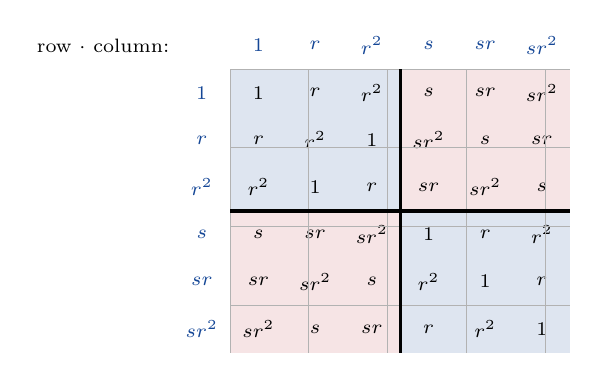
\begin{tikzpicture}[x=0.72cm,y=-0.6cm]
  \def\els{{"$1$","$r$","$r^2$","$s$","$sr$","$sr^2$"}}
  % table body: 1=rotation, 2=reflection; entries as strings
  \foreach \i/\row in {0/{1,r,r^2,s,sr,sr^2}, 1/{r,r^2,1,sr^2,s,sr}, 2/{r^2,1,r,sr,sr^2,s}, 3/{s,sr,sr^2,1,r,r^2}, 4/{sr,sr^2,s,r^2,1,r}, 5/{sr^2,s,sr,r,r^2,1}} {
    \foreach \e [count=\j from 0] in \row {
      \pgfmathtruncatemacro{\isrot}{ifthenelse(\j<3,1,0)*ifthenelse(\i<3,1,0)+ifthenelse(\j>2,1,0)*ifthenelse(\i>2,1,0)}
      \ifnum\isrot=1 \fill[big!14] (\j,\i) rectangle ++(1,1); \else \fill[pit!12] (\j,\i) rectangle ++(1,1); \fi
      \node[font=\scriptsize] at (\j+0.5,\i+0.5) {$\e$};
    } }
  \draw[gray!60] (0,0) grid (6,6);
  \draw[very thick] (3,0)--(3,6); \draw[very thick] (0,3)--(6,3);
  \foreach \e [count=\j from 0] in {1,r,r^2,s,sr,sr^2} {\node[font=\scriptsize,big] at (\j+0.5,-0.5) {$\e$}; \node[font=\scriptsize,big] at (-0.5,\j+0.5) {$\e$};}
  \node[font=\scriptsize,anchor=east] at (-0.9,-0.5) {row $\cdot$ column:};
\end{tikzpicture}}

\newcommand{\figaxes}{%
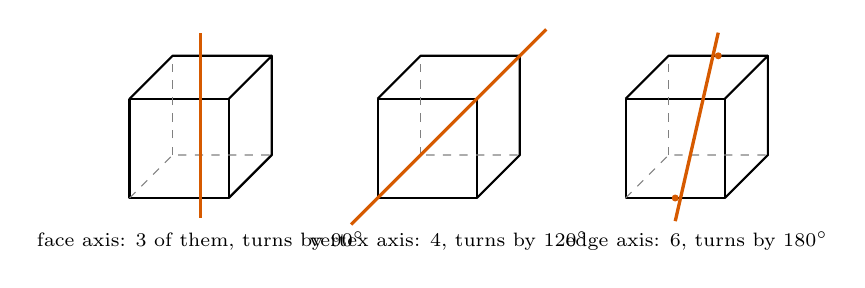
\begin{tikzpicture}[scale=0.42,line join=round]
  \foreach \dx/\axis/\cap in {0/face/{face axis: 3 of them, turns by $90^\circ$}, 7.5/vertex/{vertex axis: 4, turns by $120^\circ$}, 15/edge/{edge axis: 6, turns by $180^\circ$}} {
    \begin{scope}[xshift=\dx cm]
      \coordinate (A) at (0,0); \coordinate (B) at (3,0); \coordinate (C) at (3,3); \coordinate (D) at (0,3);
      \coordinate (E) at (1.3,1.3); \coordinate (F) at (4.3,1.3); \coordinate (G) at (4.3,4.3); \coordinate (H) at (1.3,4.3);
      \draw[thick] (A)--(B)--(C)--(D)--cycle; \draw[thick] (B)--(F)--(G)--(C); \draw[thick] (D)--(H)--(G);
      \draw[dashed,gray] (A)--(E)--(F); \draw[dashed,gray] (E)--(H);
      \node[font=\scriptsize,align=center] at (2.15,-1.3) {\cap};
    \end{scope} }
  \draw[very thick,mkc] (2.15,-0.6) -- (2.15,5.0);
  \draw[very thick,mkc] (7.5-0.8,-0.8) -- (7.5+4.3+0.8,4.3+0.8);
  \draw[very thick,mkc] (15+1.5,-0.7) -- (15+2.8,5.0);
  \fill[mkc] (15+1.5,0) circle (3pt); \fill[mkc] (15+2.8,4.3) circle (3pt);
\end{tikzpicture}}

\newcommand{\figcyclearrows}{%
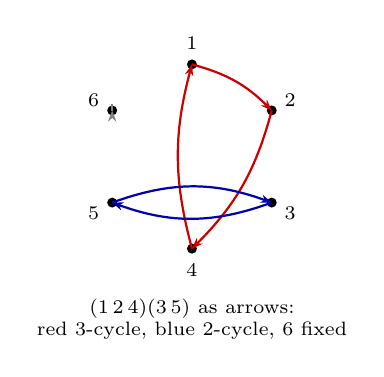
\begin{tikzpicture}[scale=0.9,>={Stealth[length=4pt]}]
  \foreach \i in {1,...,6} {\coordinate (P\i) at ({90-60*(\i-1)}:1.3); \fill (P\i) circle (2pt); \node[font=\scriptsize] at ({90-60*(\i-1)}:1.6) {\i};}
  \draw[->,thick,red!80!black] (P1) to[bend left=15] (P2);
  \draw[->,thick,red!80!black] (P2) to[bend left=15] (P4);
  \draw[->,thick,red!80!black] (P4) to[bend left=15] (P1);
  \draw[->,thick,blue!70!black] (P3) to[bend left=20] (P5);
  \draw[->,thick,blue!70!black] (P5) to[bend left=20] (P3);
  \draw[->,thick,gray] (P6) to[out=-60,in=0,looseness=6] (P6);
  \node[font=\scriptsize,align=center] at (0,-2.3) {$(1\,2\,4)(3\,5)$ as arrows:\\ red 3-cycle, blue 2-cycle, 6 fixed};
\end{tikzpicture}}

\newcommand{\figclocksub}[2]{% #1 = step k (highlight 0,k,2k,...), #2 caption
\begin{tikzpicture}[scale=0.8]
  \draw[thick,gray!60] (0,0) circle (1.2);
  \foreach \h in {0,...,11} {\fill[gray!60] ({90-30*\h}:1.2) circle (1.5pt); \node[font=\tiny] at ({90-30*\h}:1.45) {\h};}
  \pgfmathtruncatemacro{\npts}{12/#1}\pgfmathtruncatemacro{\last}{\npts-1}
  \foreach \j in {0,...,\last} {
    \pgfmathtruncatemacro{\pa}{\j*#1}\pgfmathtruncatemacro{\pb}{mod((\j+1)*#1,12)}
    \draw[thick,mkc] ({90-30*\pa}:1.2) -- ({90-30*\pb}:1.2);
    \fill[mkc] ({90-30*\pa}:1.2) circle (3pt);}
  \node[font=\scriptsize,align=center] at (0,-1.95) {#2};
\end{tikzpicture}}

\newcommand{\figsubZ}{%
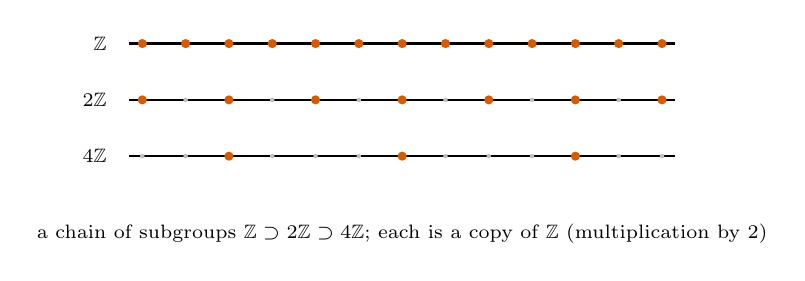
\begin{tikzpicture}[scale=0.55]
  \foreach \k/\lab/\step in {0/$\Z$/1, 1/$2\Z$/2, 2/$4\Z$/4} {
    \draw[thick] (-6.3,-1.3*\k) -- (6.3,-1.3*\k);
    \node[font=\scriptsize,anchor=east] at (-6.6,-1.3*\k) {\lab};
    \foreach \x in {-6,...,6} {\pgfmathtruncatemacro{\r}{mod(\x+12,\step)} \ifnum\r=0 \fill[mkc] (\x,-1.3*\k) circle (3pt); \else \fill[gray!50] (\x,-1.3*\k) circle (1.5pt); \fi}
  }
  \node[font=\scriptsize,align=center] at (0,-4.4) {a chain of subgroups $\Z\supset2\Z\supset4\Z$; each is a copy of $\Z$ (multiplication by $2$)};
\end{tikzpicture}}

\newcommand{\figwordpath}{%
\begin{tikzpicture}[scale=1.0,>={Stealth[length=4pt]}]
  \foreach \d/\o in {0/180,90/270,180/0,270/90} {
    \draw[gray!70] (0,0) -- (\d:2);
    \foreach \e in {0,90,180,270} {
      \ifnum\e=\o\relax\else
        \draw[gray!70] (\d:2) -- ($(\d:2)+(\e:1)$);
        \pgfmathtruncatemacro{\eo}{mod(\e+180,360)}
        \foreach \f in {0,90,180,270} {\ifnum\f=\eo\relax\else \draw[gray!50,thin] ($(\d:2)+(\e:1)$) -- ($(\d:2)+(\e:1)+(\f:0.45)$); \fi }
      \fi } }
  \fill (0,0) circle (2.5pt); \node[font=\scriptsize,below left] at (0,0) {$1$};
  \node[font=\scriptsize,below] at (2,-0.05) {$a$}; \node[font=\scriptsize,right] at (3,0) {$aa$}; \node[font=\scriptsize,right] at (2,1) {$ab$};
  % path for a a^-1 a b b^-1 a
  \draw[->,very thick,mkc] (0,0) to[bend left=35] node[above,font=\tiny] {1: $a$} (2,0);
  \draw[->,very thick,mkc] (2,0) to[bend left=35] node[below,font=\tiny] {2: $a\inv$} (0,0);
  \draw[->,very thick,mkc] (0,0) -- node[above,font=\tiny,pos=0.6] {3: $a$} (2,0);
  \draw[->,very thick,mkc] (2,0) to[bend left=35] node[left,font=\tiny] {4: $b$} (2,1);
  \draw[->,very thick,mkc] (2,1) to[bend left=35] node[right,font=\tiny] {5: $b\inv$} (2,0);
  \draw[->,very thick,mkc] (2,0) -- node[above,font=\tiny] {6: $a$} (3,0);
  \fill[mkc] (3,0) circle (3pt);
\end{tikzpicture}}

\newcommand{\figabba}{%
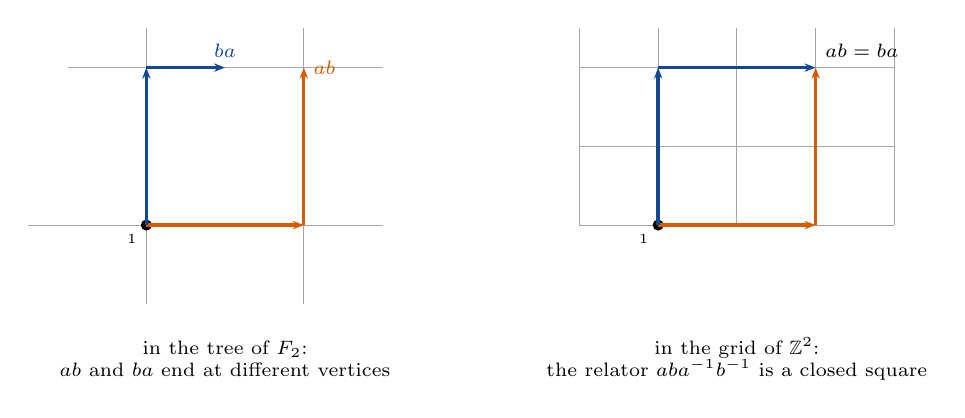
\begin{tikzpicture}[scale=1.0,>={Stealth[length=4pt]}]
  \begin{scope}
    \draw[gray!70] (-1.5,0)--(3,0); \draw[gray!70] (0,-1)--(0,2.5); \draw[gray!70] (2,-1)--(2,2.5); \draw[gray!70] (0,2)--(-1,2); \draw[gray!70] (0,2)--(1,2);
    \draw[gray!70] (2,2)--(3,2); \draw[gray!70] (2,2)--(1,2);
    \fill (0,0) circle (2pt); \node[font=\tiny,below left] at (0,0) {$1$};
    \draw[->,very thick,mkc] (0,0)--(2,0); \draw[->,very thick,mkc] (2,0)--(2,2); \node[font=\scriptsize,mkc,right] at (2,2) {$ab$};
    \draw[->,very thick,big] (0,0)--(0,2); \draw[->,very thick,big] (0,2)--(1,2); \node[font=\scriptsize,big,above] at (1,2) {$ba$};
    \node[font=\scriptsize,align=center] at (1,-1.7) {in the tree of $F_2$:\\ $ab$ and $ba$ end at different vertices};
  \end{scope}
  \begin{scope}[xshift=6.5cm]
    \draw[gray!70] (-1,0) grid (3,2.5);
    \fill (0,0) circle (2pt); \node[font=\tiny,below left] at (0,0) {$1$};
    \draw[->,very thick,mkc] (0,0)--(2,0); \draw[->,very thick,mkc] (2,0)--(2,2);
    \draw[->,very thick,big] (0,0)--(0,2); \draw[->,very thick,big] (0,2)--(2,2);
    \node[font=\scriptsize,above right] at (2,2) {$ab=ba$};
    \node[font=\scriptsize,align=center] at (1,-1.7) {in the grid of $\Z^2$:\\ the relator $aba\inv b\inv$ is a closed square};
  \end{scope}
\end{tikzpicture}}

\newcommand{\fighomdots}{%
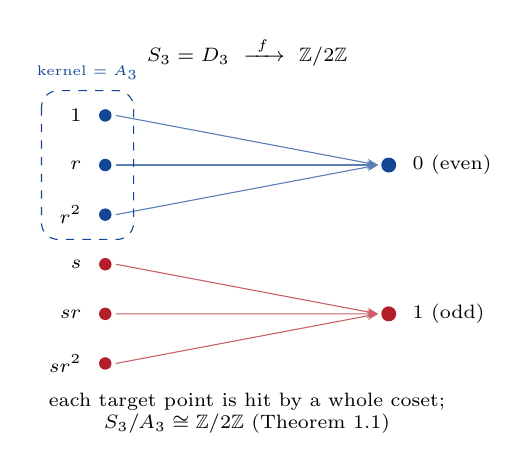
\begin{tikzpicture}[>={Stealth[length=4pt]},scale=0.9]
  \foreach \i/\l/\c in {0/1/big,1/r/big,2/r^2/big,3/s/pit,4/sr/pit,5/sr^2/pit} {
    \fill[\c] (0,-0.7*\i) circle (2.5pt); \node[font=\scriptsize,anchor=east] at (-0.2,-0.7*\i) {$\l$}; }
  \fill[big] (4,-0.7) circle (3pt); \node[font=\scriptsize,anchor=west] at (4.2,-0.7) {$0$ (even)};
  \fill[pit] (4,-2.8) circle (3pt); \node[font=\scriptsize,anchor=west] at (4.2,-2.8) {$1$ (odd)};
  \foreach \i in {0,1,2} \draw[->,big!70] (0.15,-0.7*\i) -- (3.85,-0.7);
  \foreach \i in {3,4,5} \draw[->,pit!70] (0.15,-0.7*\i) -- (3.85,-2.8);
  \draw[rounded corners=6pt,big,dashed] (-0.9,0.35) rectangle (0.4,-1.75); \node[font=\tiny,big] at (-0.25,0.6) {kernel $=A_3$};
  \node[font=\scriptsize] at (2,0.9) {$S_3=D_3\ \xrightarrow{\ f\ }\ \Z/2\Z$};
  \node[font=\scriptsize,align=center] at (2,-4.2) {each target point is hit by a whole coset;\\ $S_3/A_3\cong\Z/2\Z$ (Theorem 1.1)};
\end{tikzpicture}}

\newcommand{\figcosets}{%
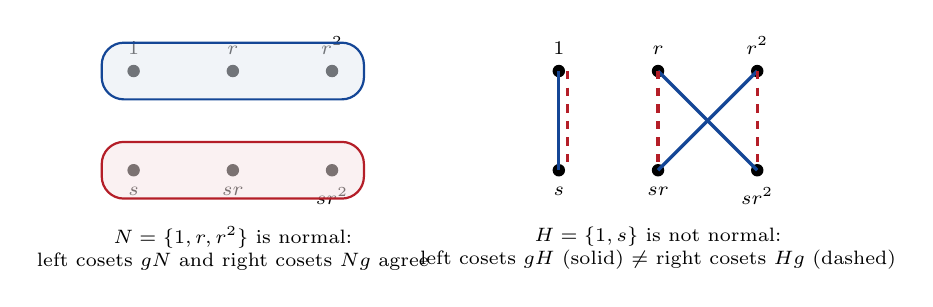
\begin{tikzpicture}[scale=0.9]
  \begin{scope}
    \foreach \j/\l in {0/1,1/r,2/r^2} {\fill (1.4*\j,0) circle (2.5pt); \node[font=\scriptsize,above] at (1.4*\j,0.1) {$\l$};}
    \foreach \j/\l in {0/s,1/sr,2/sr^2} {\fill (1.4*\j,-1.4) circle (2.5pt); \node[font=\scriptsize,below] at (1.4*\j,-1.5) {$\l$};}
    \draw[rounded corners=8pt,fill=big!12,draw=big,thick,fill opacity=0.5] (-0.45,-0.4) rectangle (3.25,0.4);
    \draw[rounded corners=8pt,fill=pit!12,draw=pit,thick,fill opacity=0.5] (-0.45,-1.8) rectangle (3.25,-1.0);
    \node[font=\scriptsize,align=center] at (1.4,-2.5) {$N=\{1,r,r^2\}$ is normal:\\ left cosets $gN$ and right cosets $Ng$ agree};
  \end{scope}
  \begin{scope}[xshift=6cm]
    \foreach \j/\l in {0/1,1/r,2/r^2} {\fill (1.4*\j,0) circle (2.5pt); \node[font=\scriptsize,above] at (1.4*\j,0.1) {$\l$};}
    \foreach \j/\l in {0/s,1/sr,2/sr^2} {\fill (1.4*\j,-1.4) circle (2.5pt); \node[font=\scriptsize,below] at (1.4*\j,-1.5) {$\l$};}
    % left cosets of H={1,s}: {1,s},{r,sr^2},{r^2,sr}  solid
    \draw[very thick,big] (0,0)--(0,-1.4);
    \draw[very thick,big] (1.4,0)--(2.8,-1.4);
    \draw[very thick,big] (2.8,0)--(1.4,-1.4);
    % right cosets: {1,s},{r,sr},{r^2,sr^2} dashed
    \draw[very thick,pit,dashed] (0.12,0)--(0.12,-1.4);
    \draw[very thick,pit,dashed] (1.4,0)--(1.4,-1.4);
    \draw[very thick,pit,dashed] (2.8,0)--(2.8,-1.4);
    \node[font=\scriptsize,align=center] at (1.4,-2.5) {$H=\{1,s\}$ is not normal:\\ left cosets $gH$ (solid) $\neq$ right cosets $Hg$ (dashed)};
  \end{scope}
\end{tikzpicture}}

\newcommand{\figcayleygallery}{%
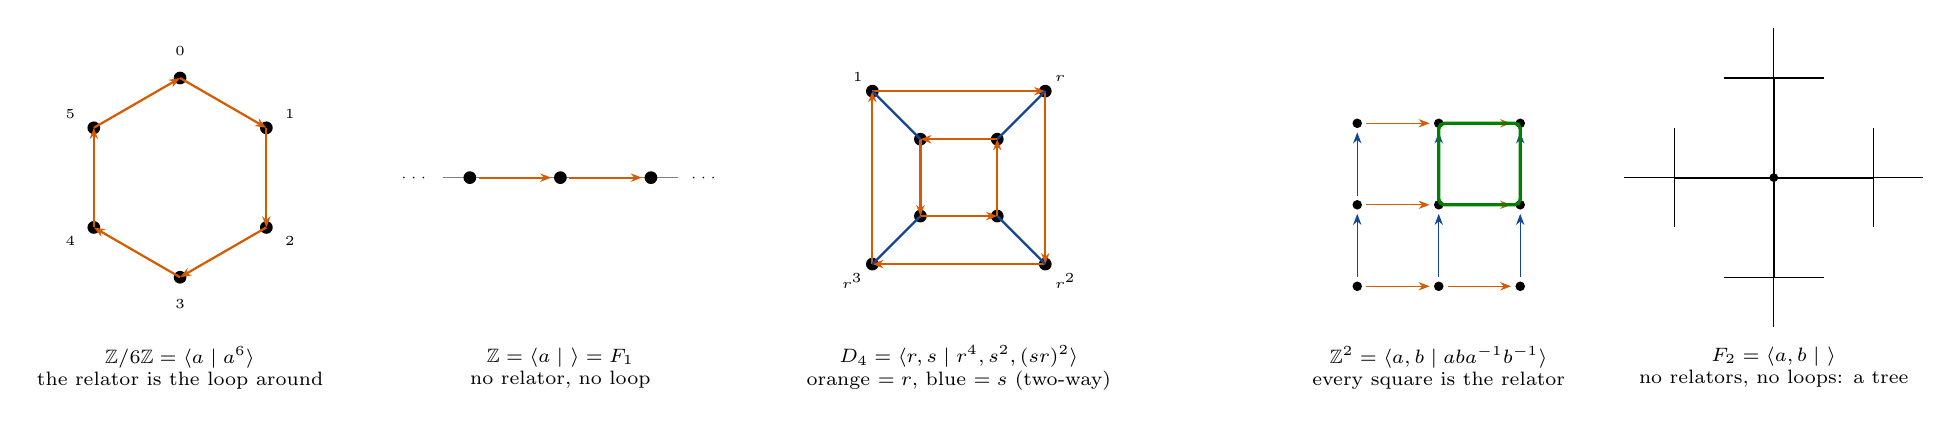
\begin{tikzpicture}[>={Stealth[length=4pt]},scale=1.15]
  % Z/6Z
  \begin{scope}
    \foreach \k in {0,...,5} {\coordinate (C\k) at ({90-60*\k}:1.1); \fill (C\k) circle (2pt); \node[font=\tiny] at ({90-60*\k}:1.4) {\k};}
    \foreach \k in {0,...,5} {\pgfmathtruncatemacro{\n}{mod(\k+1,6)} \draw[->,thick,mkc] (C\k) -- (C\n);}
    \node[font=\scriptsize,align=center] at (0,-2.1) {$\Z/6\Z=\langle a\mid a^6\rangle$\\ the relator is the loop around};
  \end{scope}
  % Z
  \begin{scope}[xshift=4.2cm]
    \draw[gray] (-1.3,0)--(1.3,0);
    \foreach \x in {-1,0,1} {\fill (\x,0) circle (2pt);}
    \foreach \x in {-1,0} \draw[->,thick,mkc] (\x+0.1,0)--(\x+0.9,0);
    \node[font=\tiny] at (-1.6,0) {$\cdots$}; \node[font=\tiny] at (1.6,0) {$\cdots$};
    \node[font=\scriptsize,align=center] at (0,-2.1) {$\Z=\langle a\mid\ \rangle=F_1$\\ no relator, no loop};
  \end{scope}
  % D4
  \begin{scope}[xshift=8.6cm]
    \foreach \k/\l in {0/1,1/r,2/r^2,3/r^3} {\coordinate (O\k) at ({135-90*\k}:1.35); \fill (O\k) circle (2pt);}
    \foreach \k/\l in {0/s,1/sr^3,2/sr^2,3/sr} {\coordinate (I\k) at ({135-90*\k}:0.6); \fill (I\k) circle (2pt);}
    \node[font=\tiny,above left] at (O0) {$1$}; \node[font=\tiny,above right] at (O1) {$r$}; \node[font=\tiny,below right] at (O2) {$r^2$}; \node[font=\tiny,below left] at (O3) {$r^3$};
    \foreach \k in {0,...,3} {\pgfmathtruncatemacro{\n}{mod(\k+1,4)} \draw[->,thick,mkc] (O\k) -- (O\n);}
    % inner: s -> sr (at I3), sr -> sr^2 (I2), sr^2 -> sr^3 (I1), sr^3 -> s (I0): reversed direction
    \foreach \k in {0,...,3} {\pgfmathtruncatemacro{\n}{mod(\k+3,4)} \draw[->,thick,mkc] (I\k) -- (I\n);}
    \foreach \k in {0,...,3} \draw[thick,big] (O\k) -- (I\k);
    \node[font=\scriptsize,align=center] at (0,-2.1) {$D_4=\langle r,s\mid r^4,s^2,(sr)^2\rangle$\\ orange $=r$, blue $=s$ (two-way)};
  \end{scope}
  % Z^2
  \begin{scope}[xshift=13cm,yshift=-1.2cm]
    \foreach \x in {0,1,2} \foreach \y in {0,1,2} \fill (\x*0.9,\y*0.9) circle (1.5pt);
    \foreach \y in {0,1,2} \foreach \x in {0,1} \draw[->,mkc] (\x*0.9+0.1,\y*0.9)--(\x*0.9+0.8,\y*0.9);
    \foreach \x in {0,1,2} \foreach \y in {0,1} \draw[->,big] (\x*0.9,\y*0.9+0.1)--(\x*0.9,\y*0.9+0.8);
    \draw[very thick,green!50!black,rounded corners=2pt] (0.9,0.9) rectangle (1.8,1.8);
    \node[font=\scriptsize,align=center] at (0.9,-0.9) {$\Z^2=\langle a,b\mid aba\inv b\inv\rangle$\\ every square is the relator};
  \end{scope}
  % F2
  \begin{scope}[xshift=17.6cm,scale=0.55]
    \foreach \d/\o in {0/180,90/270,180/0,270/90} {\draw[thick] (0,0) -- (\d:2);
      \foreach \e in {0,90,180,270} {\ifnum\e=\o\relax\else \draw (\d:2) -- ($(\d:2)+(\e:1)$); \fi}}
    \fill (0,0) circle (2.5pt);
    \node[font=\scriptsize,align=center] at (0,-3.8) {$F_2=\langle a,b\mid\ \rangle$\\ no relators, no loops: a tree};
  \end{scope}
\end{tikzpicture}}


\newcommand{\figwhypi}{%
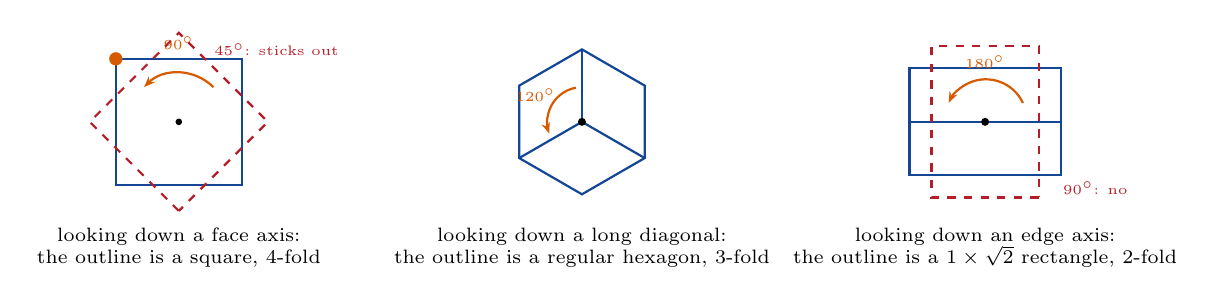
\begin{tikzpicture}[scale=0.8,>={Stealth[length=4pt]}]
  % (a) face axis: square silhouette
  \begin{scope}
    \draw[thick,big] (-1,-1) rectangle (1,1); \fill[mkc] (-1,1) circle (3pt);
    \fill (0,0) circle (1.5pt);
    \draw[->,mkc,thick] (0.55,0.55) arc (45:135:0.78);
    \node[font=\tiny,mkc] at (0,1.25) {$90^\circ$};
    \draw[thick,pit,dashed,rotate=45] (-1,-1) rectangle (1,1);
    \node[font=\tiny,pit] at (1.55,1.15) {$45^\circ$: sticks out};
    \node[font=\scriptsize,align=center] at (0,-2.0) {looking down a face axis:\\ the outline is a square, 4-fold};
  \end{scope}
  % (b) vertex axis: hexagon silhouette
  \begin{scope}[xshift=6.4cm]
    \draw[thick,big] (30:1.15)--(90:1.15)--(150:1.15)--(210:1.15)--(270:1.15)--(330:1.15)--cycle;
    \draw[thick,big] (0,0)--(90:1.15); \draw[thick,big] (0,0)--(210:1.15); \draw[thick,big] (0,0)--(330:1.15);
    \fill (0,0) circle (1.8pt);
    \draw[->,mkc,thick] (100:0.55) arc (100:200:0.55); \node[font=\tiny,mkc] at (150:0.85) {$120^\circ$};
    \node[font=\scriptsize,align=center] at (0,-2.0) {looking down a long diagonal:\\ the outline is a regular hexagon, 3-fold};
  \end{scope}
  % (c) edge axis: rectangle silhouette 1 x sqrt2
  \begin{scope}[xshift=12.8cm]
    \draw[thick,big] (-1.2,-0.85) rectangle (1.2,0.85);
    \draw[thick,big] (-1.2,0)--(1.2,0);
    \fill (0,0) circle (1.8pt);
    \draw[->,mkc,thick] (0.6,0.3) arc (25:155:0.65); \node[font=\tiny,mkc] at (0,0.95) {$180^\circ$};
    \draw[thick,pit,dashed,rotate=90] (-1.2,-0.85) rectangle (1.2,0.85);
    \node[font=\tiny,pit] at (1.75,-1.05) {$90^\circ$: no};
    \node[font=\scriptsize,align=center] at (0,-2.0) {looking down an edge axis:\\ the outline is a $1\times\sqrt2$ rectangle, 2-fold};
  \end{scope}
\end{tikzpicture}}

% =====================================================================
\begin{document}

% ---------------------------------------------------------------- COVER
\begin{textblock*}{744pt}(24pt,24pt)
{\sffamily\bfseries\huge Office Hour One: Groups}\par\vspace{4pt}
{\sffamily\Large An annotated study edition}\par\vspace{6pt}
{\large Original chapter: Matt Clay and Dan Margalit, \emph{Office Hours with a Geometric Group Theorist} (Princeton University Press, 2017), pages 3--20.}\par
\vspace{14pt}
\begin{minipage}[t]{385pt}
{\sffamily\bfseries\large How to read this}\par\vspace{4pt}
Each spread shows one original page of the chapter on the left, untouched, and a column of annotations on the right.
Orange numbered markers \num{1}\,\num{2}\,\num{3} on the page point to the line the annotation is about; a faint yellow bar
marks the exact statement when it matters.
The annotations aim at a strong high-school reader: they fill in background the authors assume (functions, modular arithmetic, matrices),
draw pictures of every construction, work examples in full, and give hints for all thirteen exercises.

\vspace{6pt}
{\sffamily\bfseries\large Colour code for the boxes}\par\vspace{2pt}
\begin{tabular}{@{}ll@{}}
\textcolor{big}{\rule{8pt}{8pt}} Big picture & where an idea sits in the whole book\\
\textcolor{why}{\rule{8pt}{8pt}} Why? & the reason a definition or claim is true\\
\textcolor{pit}{\rule{8pt}{8pt}} Watch out & a common misreading, or a slip in the printed text\\
\textcolor{try}{\rule{8pt}{8pt}} Try it & something to check by hand, and hints for exercises\\
\textcolor{ahead}{\rule{8pt}{8pt}} Looking ahead & connections to later office hours\\
\textcolor{gray!60!black}{\rule{8pt}{8pt}} Background & facts from school mathematics the text assumes\\
\end{tabular}

\vspace{10pt}
{\sffamily\bfseries\large Contents of the chapter}\par\vspace{2pt}
\begin{tabular}{@{}lll@{}}
Symmetry, the cube, and $S_4$ & book pp.\ 3--5 & spreads 1--3, A2--A5\\
1.1 Groups: $D_n$, $S_n$, $\Z/n\Z$ & book pp.\ 5--9 & spreads 3--7, B, B2\\
1.2 Infinite groups: $\Z$, $\Z^2$, matrices, free groups & book pp.\ 9--13 & spreads 7--11\\
1.3 Homomorphisms and normal subgroups & book pp.\ 13--17 & spreads 11--15\\
1.4 Group presentations & book pp.\ 17--20 & spreads 15--18\\
Visual pages V1--V5 & --- & between spreads\\
Chapter map, exercise hints, glossary & --- & closing pages\\
\end{tabular}
\end{minipage}\hfill
\begin{minipage}[t]{330pt}
\begin{bigpic}
\textbf{The one sentence to keep in mind.} The whole chapter is an argument that ``group'' and ``the symmetries of something'' are the same idea seen from two sides.
Every example is introduced twice: once as a set with a multiplication, and once as the symmetries of a picture you can draw.
Office Hour 2 turns this into a theorem (every group is the symmetry group of its Cayley graph).
\end{bigpic}
\begin{prereq}
You will get the most out of the chapter if these words already mean something to you:
\emph{function}, \emph{bijection} (one-to-one and onto), \emph{composition} $g\circ h$ (do $h$ first),
\emph{remainder} on division by $n$, \emph{vector addition}, \emph{$2\times2$ determinant} and the fact that $\det(MN)=\det M\,\det N$.
Each is reviewed in a grey box the first time the text needs it.
\end{prereq}
\vspace{6pt}
\centering \figtriangle\par
{\scriptsize A warm-up the chapter skips: the equilateral triangle has 6 symmetries, and they behave exactly like the 6 permutations of its 3 corners.}
\end{minipage}
\end{textblock*}
\mbox{}\clearpage

% ================================================================ BOOK p.3
\bookpage{018}{3}{
  \mk{1}{40}{409} \mk{2}{40}{457} \hl{55}{452}{330}{50}
  \mk{3}{40}{531}
}
\anncol{
\A{1}{``Determine the symmetries of objects''}
A \emph{symmetry} of an object is a way of moving it that leaves it looking exactly as before.
The key point the whole book builds on: symmetries can be \emph{combined} (do one, then another) and \emph{undone}.
Those two features are what the word ``group'' packages up.

\begin{prereq}
A \emph{function} $f:X\to Y$ assigns to each input one output. It is a \emph{bijection} if every element of $Y$ is hit exactly once; then it has an inverse $f\inv$.
The \emph{composition} $g\circ h$ means ``apply $h$, then $g$''. Symmetries are bijections from an object to itself, so all of this applies to them.
\end{prereq}

\A{2}{The plan of the first two office hours}
Office Hour 1 (this chapter) goes one way: start from familiar groups and show each is a set of symmetries of a picture.
Office Hour 2 goes the other way and proves it in general.
The phrase ``the interactions between them'' is the subject of geometric group theory: use the geometry of the object to learn algebra about the group, and vice versa.

\begin{bigpic}
Keep a running list as you read. For each group met in this chapter, write down (a) the set, (b) the multiplication, (c) the object it is the symmetries of.
By the end you should have about ten rows. That table \emph{is} the content of the chapter.
\end{bigpic}

\A{3}{The cube}
The chapter's first worked example. Before turning the page, try to answer the question yourself: how many ways can you pick up a cube, turn it, and put it back down so that it occupies the same place?
(Turning is allowed; mirror-reversing is not.) Count the ones you can find; the next page shows there are 24 and, better, explains what the 24 ``are''.

\begin{tryit}
Do the same for a square drawn on paper, allowing only rotations of the paper: you should find 4. Allowing flips as well gives 8. Both answers reappear on page 6 as $\Z/4\Z$ and $D_4$.
\end{tryit}
}

% ================================================================ BOOK p.4
\bookpage{019}{4}{
  \mk{1}{52}{72} \mk{2}{52}{192} \hl{67}{184}{300}{34}
  \mk{3}{52}{264} \mk{4}{52}{410} \mk{5}{52}{467} \mk{6}{52}{548} \hl{67}{540}{320}{12}
}
\anncol{
\A{1}{``Rigid transformation, no reflections''}
Rigid means distances are preserved: the cube is moved as a solid body, not squashed.
Reflections are excluded because you cannot perform a mirror image with your hands; a transformation you \emph{can} perform is called \emph{orientation-preserving}.
If reflections were allowed the count would double to 48.

\A{2}{The count $8\times3=24$}
Fix one corner $A$. A symmetry must send $A$ to one of the 8 corners. Once you know where $A$ goes, the cube can still spin about the long diagonal through that corner, and there are exactly 3 positions (rotate by $0^\circ$, $120^\circ$, $240^\circ$) that fit. Every symmetry is determined by these two choices, so there are $8\cdot 3=24$.
The complaint that follows is the important one: counting is not understanding. We want to know how the 24 combine.

\A{3}{The four long diagonals}
A long diagonal joins a corner to the opposite corner through the centre of the cube. See Interlude A2, two spreads on, for a labelled picture: $d_1=AG$, $d_2=BH$, $d_3=CE$, $d_4=DF$.

\A{4}{The two facts}
\emph{First fact.} A symmetry moves corners to corners and keeps opposite corners opposite, so it sends each long diagonal to a long diagonal; that is a rearrangement (permutation) of $\{d_1,d_2,d_3,d_4\}$.

\emph{Second fact, existence part.} Take two diagonals, say $d_1=AG$ and $d_2=BH$. The edge $AB$ joins an endpoint of each, and so does the opposite edge $GH$. Rotating by $180^\circ$ about the axis through the midpoints of $AB$ and $GH$ swaps $A\leftrightarrow B$ and $G\leftrightarrow H$, hence swaps $d_1\leftrightarrow d_2$, and it fixes the other two diagonals. So every ``swap two diagonals'' is realised; and any permutation is a product of swaps (page 7), so every permutation is realised.

\begin{why}
\emph{Uniqueness} is quietly handled by counting: the map $\{\text{symmetries}\}\to\{\text{permutations of 4 diagonals}\}$ is onto, both sets have 24 elements, so it is a bijection. A direct argument: a symmetry fixing all four diagonals must fix or flip each of them; a little geometry shows only the identity does so.
\end{why}

\A{5}{``Skewering through the midpoints of two edges''}
This is the edge-axis half turn drawn in Interlude A4 and listed in the dictionary of Interlude B2. There are 6 pairs of opposite edges, giving the 6 transpositions of $S_4$.

\A{6}{$4!=24$ and composition}
$4!=4\cdot3\cdot2\cdot1$ counts the ways to arrange 4 things in order: 4 choices for where $d_1$ goes, then 3, then 2, then 1.
The final sentence is the real payoff: since a permutation is a function, ``do one symmetry then another'' becomes ``compose two functions'', which is completely mechanical. The cube's symmetries are no longer a bag of 24 moves but a structured object, $S_4$.
}

% ================================================================ INTERLUDE A2 (face axis)
\interlude{A2. Face axes: three turns about each}{
\begin{minipage}[t]{744pt}\vspace{0pt}
\begin{minipage}[t]{530pt}\vspace{0pt}\small
Each turn is shown three ways. Left: the cube \emph{before} (every label in its home corner) and \emph{after} (every label drawn in the corner its point has moved to). Each corner has its own colour and the colour travels with the label, so the shifted pattern of colours shows the turn at a glance; a corner on the axis keeps its colour in place. Middle: the same turn seen from directly above the axis, where it is a flat rotation of an outline. Right: the corner moves and the resulting permutation of the diagonals $d_1=AG$, $d_2=BH$, $d_3=CE$, $d_4=DF$. The orange line is the axis, the orange arc the direction of the turn. The cube on the right shows all three face axes; the rows below use the top--bottom one.
\end{minipage}\hfill
\begin{minipage}[t]{200pt}\vspace{0pt}\centering
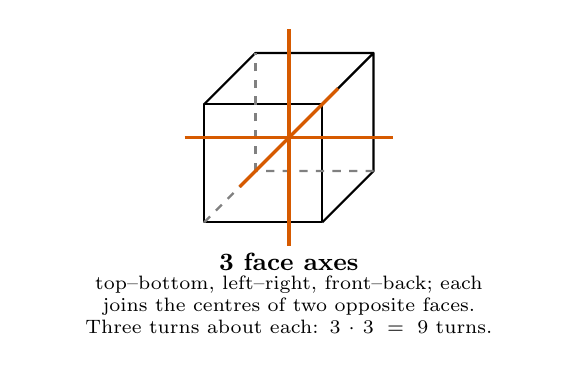
\begin{tikzpicture}[scale=0.5,line join=round]
  \draw[thick] (0,0)--(3,0)--(3,3)--(0,3)--cycle; \draw[thick] (3,0)--(4.3,1.3)--(4.3,4.3)--(3,3); \draw[thick] (0,3)--(1.3,4.3)--(4.3,4.3);
  \draw[thick,dashed,gray] (0,0)--(1.3,1.3)--(4.3,1.3); \draw[thick,dashed,gray] (1.3,1.3)--(1.3,4.3);
  \draw[very thick,mkc] (2.15,-0.6)--(2.15,4.9);
  \draw[very thick,mkc] (-0.5,2.15)--(4.8,2.15);
  \draw[very thick,mkc] (0.9,0.9)--(3.4,3.4);
  \node[font=\small\bfseries] at (2.15,-1.0) {3 face axes};
  \node[font=\scriptsize,align=center,text width=6.4cm] at (2.15,-2.1) {top--bottom, left--right, front--back; each joins the centres of two opposite faces. Three turns about each: $3\cdot3=9$ turns.};
\end{tikzpicture}
\end{minipage}\par\vspace{4pt}
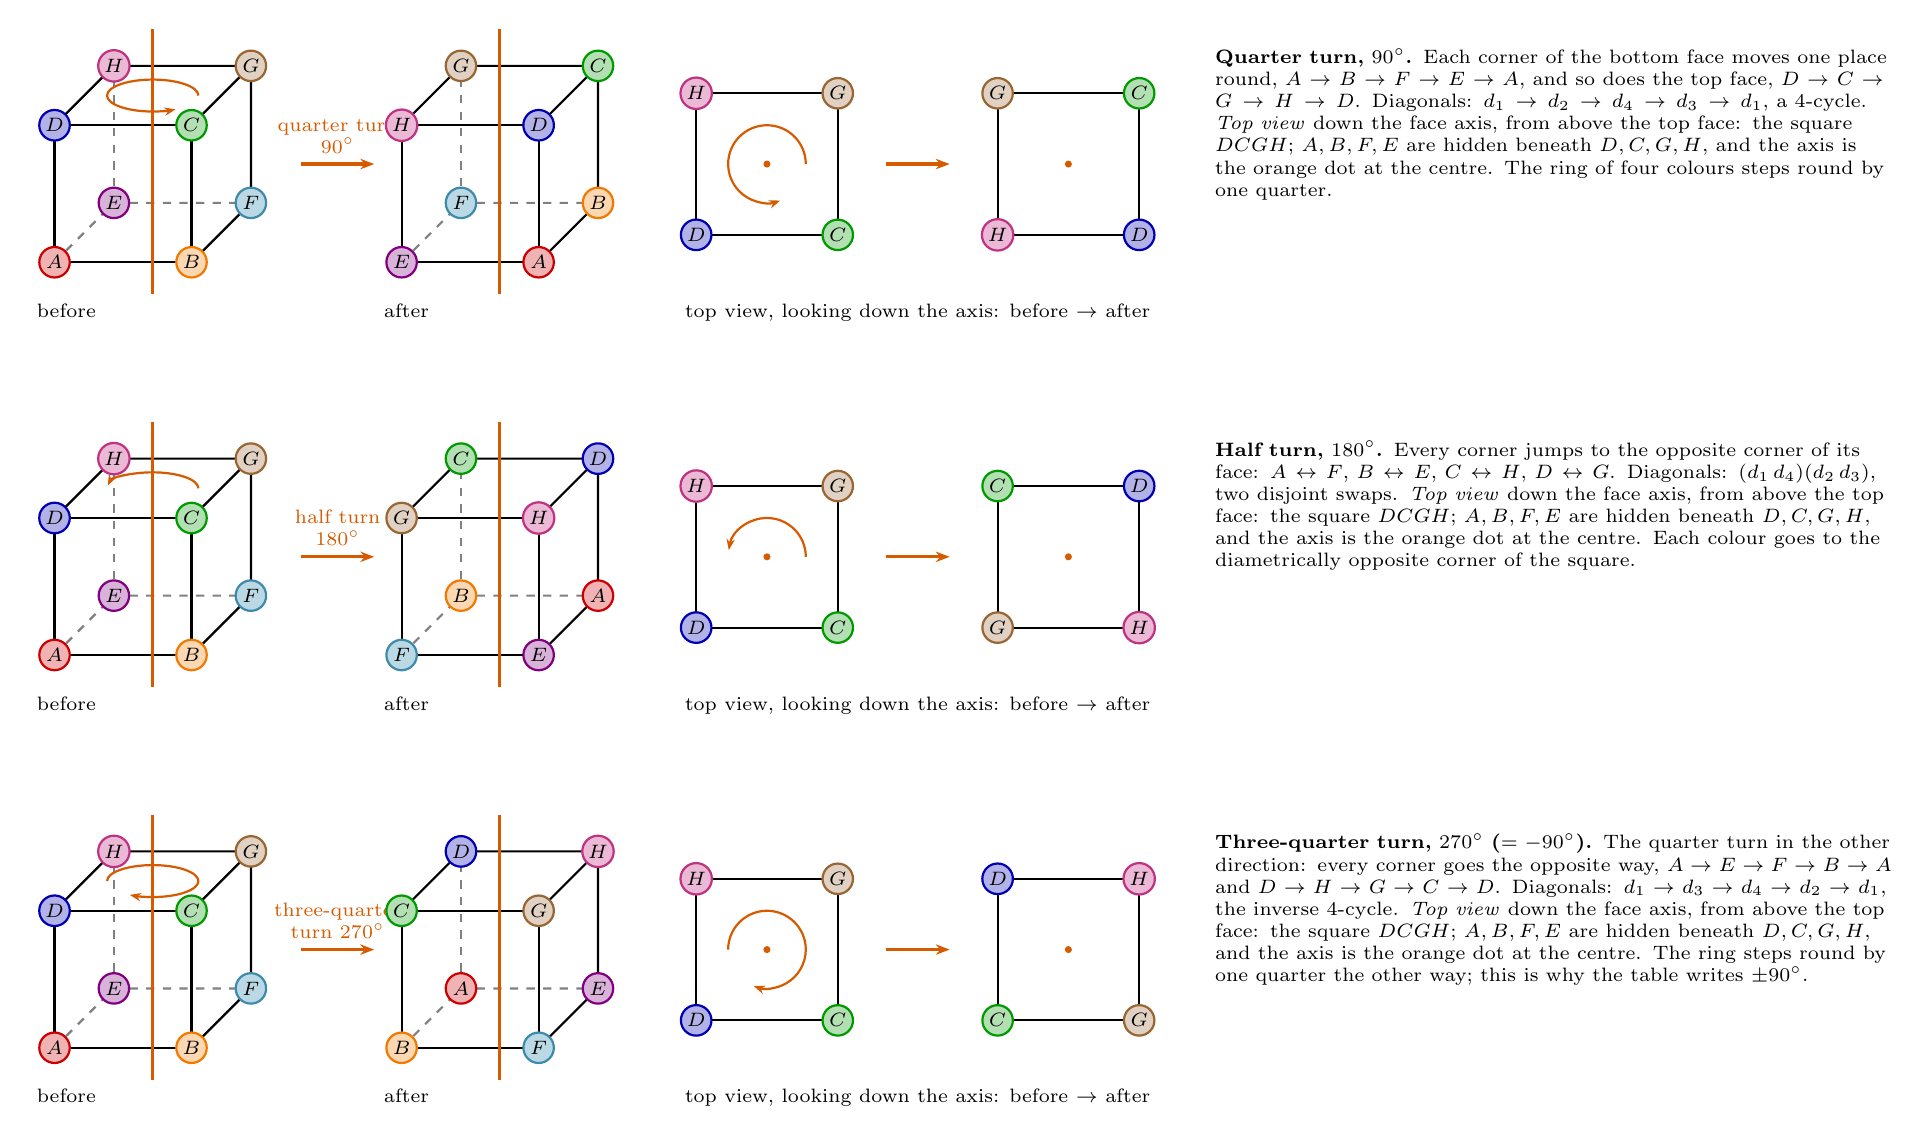
\begin{tikzpicture}[scale=0.58,line join=round]
\begin{scope}[shift={(0,0)}]
  \draw[thick] (0,0)--(3,0)--(3,3)--(0,3)--cycle; \draw[thick] (3,0)--(4.3,1.3)--(4.3,4.3)--(3,3); \draw[thick] (0,3)--(1.3,4.3)--(4.3,4.3);
  \draw[thick,dashed,gray] (0,0)--(1.3,1.3)--(4.3,1.3); \draw[thick,dashed,gray] (1.3,1.3)--(1.3,4.3);
  \draw[very thick,mkc] (2.15,-0.7)--(2.15,5.1);
  \draw[-{Stealth[length=4pt]},mkc,thick] (3.15,3.65) arc (0:300:1.0 and 0.35);
  \node[font=\scriptsize\bfseries,circle,inner sep=1pt,minimum size=11pt,fill=red!80!black!30,draw=red!80!black,thick,text=black] at (0,0) {$A$};
  \node[font=\scriptsize\bfseries,circle,inner sep=1pt,minimum size=11pt,fill=orange!95!black!30,draw=orange!95!black,thick,text=black] at (3,0) {$B$};
  \node[font=\scriptsize\bfseries,circle,inner sep=1pt,minimum size=11pt,fill=green!60!black!30,draw=green!60!black,thick,text=black] at (3,3) {$C$};
  \node[font=\scriptsize\bfseries,circle,inner sep=1pt,minimum size=11pt,fill=blue!70!black!30,draw=blue!70!black,thick,text=black] at (0,3) {$D$};
  \node[font=\scriptsize\bfseries,circle,inner sep=1pt,minimum size=11pt,fill=violet!30,draw=violet,thick,text=black] at (1.3,1.3) {$E$};
  \node[font=\scriptsize\bfseries,circle,inner sep=1pt,minimum size=11pt,fill=cyan!65!black!30,draw=cyan!65!black,thick,text=black] at (4.3,1.3) {$F$};
  \node[font=\scriptsize\bfseries,circle,inner sep=1pt,minimum size=11pt,fill=brown!80!black!30,draw=brown!80!black,thick,text=black] at (4.3,4.3) {$G$};
  \node[font=\scriptsize\bfseries,circle,inner sep=1pt,minimum size=11pt,fill=magenta!75!black!30,draw=magenta!75!black,thick,text=black] at (1.3,4.3) {$H$};
\end{scope}
  \draw[-{Stealth[length=5pt]},very thick,mkc] (5.4,2.15) -- node[above,font=\scriptsize,mkc,align=center] {quarter turn\\$90^\circ$} (7.0,2.15);
\begin{scope}[shift={(7.6,0)}]
  \draw[thick] (0,0)--(3,0)--(3,3)--(0,3)--cycle; \draw[thick] (3,0)--(4.3,1.3)--(4.3,4.3)--(3,3); \draw[thick] (0,3)--(1.3,4.3)--(4.3,4.3);
  \draw[thick,dashed,gray] (0,0)--(1.3,1.3)--(4.3,1.3); \draw[thick,dashed,gray] (1.3,1.3)--(1.3,4.3);
  \draw[very thick,mkc] (2.15,-0.7)--(2.15,5.1);
  \node[font=\scriptsize\bfseries,circle,inner sep=1pt,minimum size=11pt,fill=red!80!black!30,draw=red!80!black,thick,text=black] at (3,0) {$A$};
  \node[font=\scriptsize\bfseries,circle,inner sep=1pt,minimum size=11pt,fill=orange!95!black!30,draw=orange!95!black,thick,text=black] at (4.3,1.3) {$B$};
  \node[font=\scriptsize\bfseries,circle,inner sep=1pt,minimum size=11pt,fill=cyan!65!black!30,draw=cyan!65!black,thick,text=black] at (1.3,1.3) {$F$};
  \node[font=\scriptsize\bfseries,circle,inner sep=1pt,minimum size=11pt,fill=violet!30,draw=violet,thick,text=black] at (0,0) {$E$};
  \node[font=\scriptsize\bfseries,circle,inner sep=1pt,minimum size=11pt,fill=blue!70!black!30,draw=blue!70!black,thick,text=black] at (3,3) {$D$};
  \node[font=\scriptsize\bfseries,circle,inner sep=1pt,minimum size=11pt,fill=green!60!black!30,draw=green!60!black,thick,text=black] at (4.3,4.3) {$C$};
  \node[font=\scriptsize\bfseries,circle,inner sep=1pt,minimum size=11pt,fill=brown!80!black!30,draw=brown!80!black,thick,text=black] at (1.3,4.3) {$G$};
  \node[font=\scriptsize\bfseries,circle,inner sep=1pt,minimum size=11pt,fill=magenta!75!black!30,draw=magenta!75!black,thick,text=black] at (0,3) {$H$};
\end{scope}
  \node[font=\scriptsize,anchor=north west] at (-0.6,-0.7) {before};
  \node[font=\scriptsize,anchor=north west] at (7.0,-0.7) {after};
\begin{scope}[shift={(15.6,2.15)}]
  \draw[thick] (-1.55,-1.55) rectangle (1.55,1.55);
  \fill[mkc] (0,0) circle (2.2pt);
  \draw[-{Stealth[length=4pt]},mkc,thick] (0.85,0) arc (0:290:0.85);
  \node[font=\scriptsize\bfseries,circle,inner sep=1pt,minimum size=11pt,fill=blue!70!black!30,draw=blue!70!black,thick,text=black] at (-1.55,-1.55) {$D$};
  \node[font=\scriptsize\bfseries,circle,inner sep=1pt,minimum size=11pt,fill=green!60!black!30,draw=green!60!black,thick,text=black] at (1.55,-1.55) {$C$};
  \node[font=\scriptsize\bfseries,circle,inner sep=1pt,minimum size=11pt,fill=brown!80!black!30,draw=brown!80!black,thick,text=black] at (1.55,1.55) {$G$};
  \node[font=\scriptsize\bfseries,circle,inner sep=1pt,minimum size=11pt,fill=magenta!75!black!30,draw=magenta!75!black,thick,text=black] at (-1.55,1.55) {$H$};
\end{scope}
  \draw[-{Stealth[length=5pt]},very thick,mkc] (18.2,2.15) -- (19.6,2.15);
\begin{scope}[shift={(22.2,2.15)}]
  \draw[thick] (-1.55,-1.55) rectangle (1.55,1.55);
  \fill[mkc] (0,0) circle (2.2pt);
  \node[font=\scriptsize\bfseries,circle,inner sep=1pt,minimum size=11pt,fill=magenta!75!black!30,draw=magenta!75!black,thick,text=black] at (-1.55,-1.55) {$H$};
  \node[font=\scriptsize\bfseries,circle,inner sep=1pt,minimum size=11pt,fill=blue!70!black!30,draw=blue!70!black,thick,text=black] at (1.55,-1.55) {$D$};
  \node[font=\scriptsize\bfseries,circle,inner sep=1pt,minimum size=11pt,fill=green!60!black!30,draw=green!60!black,thick,text=black] at (1.55,1.55) {$C$};
  \node[font=\scriptsize\bfseries,circle,inner sep=1pt,minimum size=11pt,fill=brown!80!black!30,draw=brown!80!black,thick,text=black] at (-1.55,1.55) {$G$};
\end{scope}
  \node[font=\scriptsize,anchor=north] at (18.9,-0.7) {top view, looking down the axis: before $\to$ after};
  \node[font=\scriptsize,align=left,text width=8.6cm,anchor=north west] at (25.2,4.9) {\textbf{Quarter turn, $90^\circ$.} Each corner of the bottom face moves one place round, $A\to B\to F\to E\to A$, and so does the top face, $D\to C\to G\to H\to D$. Diagonals: $d_1\to d_2\to d_4\to d_3\to d_1$, a 4-cycle. \emph{Top view} down the face axis, from above the top face: the square $DCGH$; $A,B,F,E$ are hidden beneath $D,C,G,H$, and the axis is the orange dot at the centre. The ring of four colours steps round by one quarter.};
\begin{scope}[shift={(0,-8.6)}]
  \draw[thick] (0,0)--(3,0)--(3,3)--(0,3)--cycle; \draw[thick] (3,0)--(4.3,1.3)--(4.3,4.3)--(3,3); \draw[thick] (0,3)--(1.3,4.3)--(4.3,4.3);
  \draw[thick,dashed,gray] (0,0)--(1.3,1.3)--(4.3,1.3); \draw[thick,dashed,gray] (1.3,1.3)--(1.3,4.3);
  \draw[very thick,mkc] (2.15,-0.7)--(2.15,5.1);
  \draw[-{Stealth[length=4pt]},mkc,thick] (3.15,3.65) arc (0:170:1.0 and 0.35);
  \node[font=\scriptsize\bfseries,circle,inner sep=1pt,minimum size=11pt,fill=red!80!black!30,draw=red!80!black,thick,text=black] at (0,0) {$A$};
  \node[font=\scriptsize\bfseries,circle,inner sep=1pt,minimum size=11pt,fill=orange!95!black!30,draw=orange!95!black,thick,text=black] at (3,0) {$B$};
  \node[font=\scriptsize\bfseries,circle,inner sep=1pt,minimum size=11pt,fill=green!60!black!30,draw=green!60!black,thick,text=black] at (3,3) {$C$};
  \node[font=\scriptsize\bfseries,circle,inner sep=1pt,minimum size=11pt,fill=blue!70!black!30,draw=blue!70!black,thick,text=black] at (0,3) {$D$};
  \node[font=\scriptsize\bfseries,circle,inner sep=1pt,minimum size=11pt,fill=violet!30,draw=violet,thick,text=black] at (1.3,1.3) {$E$};
  \node[font=\scriptsize\bfseries,circle,inner sep=1pt,minimum size=11pt,fill=cyan!65!black!30,draw=cyan!65!black,thick,text=black] at (4.3,1.3) {$F$};
  \node[font=\scriptsize\bfseries,circle,inner sep=1pt,minimum size=11pt,fill=brown!80!black!30,draw=brown!80!black,thick,text=black] at (4.3,4.3) {$G$};
  \node[font=\scriptsize\bfseries,circle,inner sep=1pt,minimum size=11pt,fill=magenta!75!black!30,draw=magenta!75!black,thick,text=black] at (1.3,4.3) {$H$};
\end{scope}
  \draw[-{Stealth[length=5pt]},very thick,mkc] (5.4,-6.45) -- node[above,font=\scriptsize,mkc,align=center] {half turn\\$180^\circ$} (7.0,-6.45);
\begin{scope}[shift={(7.6,-8.6)}]
  \draw[thick] (0,0)--(3,0)--(3,3)--(0,3)--cycle; \draw[thick] (3,0)--(4.3,1.3)--(4.3,4.3)--(3,3); \draw[thick] (0,3)--(1.3,4.3)--(4.3,4.3);
  \draw[thick,dashed,gray] (0,0)--(1.3,1.3)--(4.3,1.3); \draw[thick,dashed,gray] (1.3,1.3)--(1.3,4.3);
  \draw[very thick,mkc] (2.15,-0.7)--(2.15,5.1);
  \node[font=\scriptsize\bfseries,circle,inner sep=1pt,minimum size=11pt,fill=red!80!black!30,draw=red!80!black,thick,text=black] at (4.3,1.3) {$A$};
  \node[font=\scriptsize\bfseries,circle,inner sep=1pt,minimum size=11pt,fill=cyan!65!black!30,draw=cyan!65!black,thick,text=black] at (0,0) {$F$};
  \node[font=\scriptsize\bfseries,circle,inner sep=1pt,minimum size=11pt,fill=orange!95!black!30,draw=orange!95!black,thick,text=black] at (1.3,1.3) {$B$};
  \node[font=\scriptsize\bfseries,circle,inner sep=1pt,minimum size=11pt,fill=violet!30,draw=violet,thick,text=black] at (3,0) {$E$};
  \node[font=\scriptsize\bfseries,circle,inner sep=1pt,minimum size=11pt,fill=green!60!black!30,draw=green!60!black,thick,text=black] at (1.3,4.3) {$C$};
  \node[font=\scriptsize\bfseries,circle,inner sep=1pt,minimum size=11pt,fill=magenta!75!black!30,draw=magenta!75!black,thick,text=black] at (3,3) {$H$};
  \node[font=\scriptsize\bfseries,circle,inner sep=1pt,minimum size=11pt,fill=blue!70!black!30,draw=blue!70!black,thick,text=black] at (4.3,4.3) {$D$};
  \node[font=\scriptsize\bfseries,circle,inner sep=1pt,minimum size=11pt,fill=brown!80!black!30,draw=brown!80!black,thick,text=black] at (0,3) {$G$};
\end{scope}
  \node[font=\scriptsize,anchor=north west] at (-0.6,-9.3) {before};
  \node[font=\scriptsize,anchor=north west] at (7.0,-9.3) {after};
\begin{scope}[shift={(15.6,-6.45)}]
  \draw[thick] (-1.55,-1.55) rectangle (1.55,1.55);
  \fill[mkc] (0,0) circle (2.2pt);
  \draw[-{Stealth[length=4pt]},mkc,thick] (0.85,0) arc (0:170:0.85);
  \node[font=\scriptsize\bfseries,circle,inner sep=1pt,minimum size=11pt,fill=blue!70!black!30,draw=blue!70!black,thick,text=black] at (-1.55,-1.55) {$D$};
  \node[font=\scriptsize\bfseries,circle,inner sep=1pt,minimum size=11pt,fill=green!60!black!30,draw=green!60!black,thick,text=black] at (1.55,-1.55) {$C$};
  \node[font=\scriptsize\bfseries,circle,inner sep=1pt,minimum size=11pt,fill=brown!80!black!30,draw=brown!80!black,thick,text=black] at (1.55,1.55) {$G$};
  \node[font=\scriptsize\bfseries,circle,inner sep=1pt,minimum size=11pt,fill=magenta!75!black!30,draw=magenta!75!black,thick,text=black] at (-1.55,1.55) {$H$};
\end{scope}
  \draw[-{Stealth[length=5pt]},very thick,mkc] (18.2,-6.45) -- (19.6,-6.45);
\begin{scope}[shift={(22.2,-6.45)}]
  \draw[thick] (-1.55,-1.55) rectangle (1.55,1.55);
  \fill[mkc] (0,0) circle (2.2pt);
  \node[font=\scriptsize\bfseries,circle,inner sep=1pt,minimum size=11pt,fill=brown!80!black!30,draw=brown!80!black,thick,text=black] at (-1.55,-1.55) {$G$};
  \node[font=\scriptsize\bfseries,circle,inner sep=1pt,minimum size=11pt,fill=magenta!75!black!30,draw=magenta!75!black,thick,text=black] at (1.55,-1.55) {$H$};
  \node[font=\scriptsize\bfseries,circle,inner sep=1pt,minimum size=11pt,fill=blue!70!black!30,draw=blue!70!black,thick,text=black] at (1.55,1.55) {$D$};
  \node[font=\scriptsize\bfseries,circle,inner sep=1pt,minimum size=11pt,fill=green!60!black!30,draw=green!60!black,thick,text=black] at (-1.55,1.55) {$C$};
\end{scope}
  \node[font=\scriptsize,anchor=north] at (18.9,-9.3) {top view, looking down the axis: before $\to$ after};
  \node[font=\scriptsize,align=left,text width=8.6cm,anchor=north west] at (25.2,-3.7) {\textbf{Half turn, $180^\circ$.} Every corner jumps to the opposite corner of its face: $A\leftrightarrow F$, $B\leftrightarrow E$, $C\leftrightarrow H$, $D\leftrightarrow G$. Diagonals: $(d_1\,d_4)(d_2\,d_3)$, two disjoint swaps. \emph{Top view} down the face axis, from above the top face: the square $DCGH$; $A,B,F,E$ are hidden beneath $D,C,G,H$, and the axis is the orange dot at the centre. Each colour goes to the diametrically opposite corner of the square.};
\begin{scope}[shift={(0,-17.2)}]
  \draw[thick] (0,0)--(3,0)--(3,3)--(0,3)--cycle; \draw[thick] (3,0)--(4.3,1.3)--(4.3,4.3)--(3,3); \draw[thick] (0,3)--(1.3,4.3)--(4.3,4.3);
  \draw[thick,dashed,gray] (0,0)--(1.3,1.3)--(4.3,1.3); \draw[thick,dashed,gray] (1.3,1.3)--(1.3,4.3);
  \draw[very thick,mkc] (2.15,-0.7)--(2.15,5.1);
  \draw[-{Stealth[length=4pt]},mkc,thick] (1.15,3.65) arc (180:-120:1.0 and 0.35);
  \node[font=\scriptsize\bfseries,circle,inner sep=1pt,minimum size=11pt,fill=red!80!black!30,draw=red!80!black,thick,text=black] at (0,0) {$A$};
  \node[font=\scriptsize\bfseries,circle,inner sep=1pt,minimum size=11pt,fill=orange!95!black!30,draw=orange!95!black,thick,text=black] at (3,0) {$B$};
  \node[font=\scriptsize\bfseries,circle,inner sep=1pt,minimum size=11pt,fill=green!60!black!30,draw=green!60!black,thick,text=black] at (3,3) {$C$};
  \node[font=\scriptsize\bfseries,circle,inner sep=1pt,minimum size=11pt,fill=blue!70!black!30,draw=blue!70!black,thick,text=black] at (0,3) {$D$};
  \node[font=\scriptsize\bfseries,circle,inner sep=1pt,minimum size=11pt,fill=violet!30,draw=violet,thick,text=black] at (1.3,1.3) {$E$};
  \node[font=\scriptsize\bfseries,circle,inner sep=1pt,minimum size=11pt,fill=cyan!65!black!30,draw=cyan!65!black,thick,text=black] at (4.3,1.3) {$F$};
  \node[font=\scriptsize\bfseries,circle,inner sep=1pt,minimum size=11pt,fill=brown!80!black!30,draw=brown!80!black,thick,text=black] at (4.3,4.3) {$G$};
  \node[font=\scriptsize\bfseries,circle,inner sep=1pt,minimum size=11pt,fill=magenta!75!black!30,draw=magenta!75!black,thick,text=black] at (1.3,4.3) {$H$};
\end{scope}
  \draw[-{Stealth[length=5pt]},very thick,mkc] (5.4,-15.05) -- node[above,font=\scriptsize,mkc,align=center] {three-quarter\\turn $270^\circ$} (7.0,-15.05);
\begin{scope}[shift={(7.6,-17.2)}]
  \draw[thick] (0,0)--(3,0)--(3,3)--(0,3)--cycle; \draw[thick] (3,0)--(4.3,1.3)--(4.3,4.3)--(3,3); \draw[thick] (0,3)--(1.3,4.3)--(4.3,4.3);
  \draw[thick,dashed,gray] (0,0)--(1.3,1.3)--(4.3,1.3); \draw[thick,dashed,gray] (1.3,1.3)--(1.3,4.3);
  \draw[very thick,mkc] (2.15,-0.7)--(2.15,5.1);
  \node[font=\scriptsize\bfseries,circle,inner sep=1pt,minimum size=11pt,fill=orange!95!black!30,draw=orange!95!black,thick,text=black] at (0,0) {$B$};
  \node[font=\scriptsize\bfseries,circle,inner sep=1pt,minimum size=11pt,fill=cyan!65!black!30,draw=cyan!65!black,thick,text=black] at (3,0) {$F$};
  \node[font=\scriptsize\bfseries,circle,inner sep=1pt,minimum size=11pt,fill=violet!30,draw=violet,thick,text=black] at (4.3,1.3) {$E$};
  \node[font=\scriptsize\bfseries,circle,inner sep=1pt,minimum size=11pt,fill=red!80!black!30,draw=red!80!black,thick,text=black] at (1.3,1.3) {$A$};
  \node[font=\scriptsize\bfseries,circle,inner sep=1pt,minimum size=11pt,fill=green!60!black!30,draw=green!60!black,thick,text=black] at (0,3) {$C$};
  \node[font=\scriptsize\bfseries,circle,inner sep=1pt,minimum size=11pt,fill=brown!80!black!30,draw=brown!80!black,thick,text=black] at (3,3) {$G$};
  \node[font=\scriptsize\bfseries,circle,inner sep=1pt,minimum size=11pt,fill=magenta!75!black!30,draw=magenta!75!black,thick,text=black] at (4.3,4.3) {$H$};
  \node[font=\scriptsize\bfseries,circle,inner sep=1pt,minimum size=11pt,fill=blue!70!black!30,draw=blue!70!black,thick,text=black] at (1.3,4.3) {$D$};
\end{scope}
  \node[font=\scriptsize,anchor=north west] at (-0.6,-17.9) {before};
  \node[font=\scriptsize,anchor=north west] at (7.0,-17.9) {after};
\begin{scope}[shift={(15.6,-15.05)}]
  \draw[thick] (-1.55,-1.55) rectangle (1.55,1.55);
  \fill[mkc] (0,0) circle (2.2pt);
  \draw[-{Stealth[length=4pt]},mkc,thick] (-0.85,0) arc (180:-110:0.85);
  \node[font=\scriptsize\bfseries,circle,inner sep=1pt,minimum size=11pt,fill=blue!70!black!30,draw=blue!70!black,thick,text=black] at (-1.55,-1.55) {$D$};
  \node[font=\scriptsize\bfseries,circle,inner sep=1pt,minimum size=11pt,fill=green!60!black!30,draw=green!60!black,thick,text=black] at (1.55,-1.55) {$C$};
  \node[font=\scriptsize\bfseries,circle,inner sep=1pt,minimum size=11pt,fill=brown!80!black!30,draw=brown!80!black,thick,text=black] at (1.55,1.55) {$G$};
  \node[font=\scriptsize\bfseries,circle,inner sep=1pt,minimum size=11pt,fill=magenta!75!black!30,draw=magenta!75!black,thick,text=black] at (-1.55,1.55) {$H$};
\end{scope}
  \draw[-{Stealth[length=5pt]},very thick,mkc] (18.2,-15.05) -- (19.6,-15.05);
\begin{scope}[shift={(22.2,-15.05)}]
  \draw[thick] (-1.55,-1.55) rectangle (1.55,1.55);
  \fill[mkc] (0,0) circle (2.2pt);
  \node[font=\scriptsize\bfseries,circle,inner sep=1pt,minimum size=11pt,fill=green!60!black!30,draw=green!60!black,thick,text=black] at (-1.55,-1.55) {$C$};
  \node[font=\scriptsize\bfseries,circle,inner sep=1pt,minimum size=11pt,fill=brown!80!black!30,draw=brown!80!black,thick,text=black] at (1.55,-1.55) {$G$};
  \node[font=\scriptsize\bfseries,circle,inner sep=1pt,minimum size=11pt,fill=magenta!75!black!30,draw=magenta!75!black,thick,text=black] at (1.55,1.55) {$H$};
  \node[font=\scriptsize\bfseries,circle,inner sep=1pt,minimum size=11pt,fill=blue!70!black!30,draw=blue!70!black,thick,text=black] at (-1.55,1.55) {$D$};
\end{scope}
  \node[font=\scriptsize,anchor=north] at (18.9,-17.9) {top view, looking down the axis: before $\to$ after};
  \node[font=\scriptsize,align=left,text width=8.6cm,anchor=north west] at (25.2,-12.3) {\textbf{Three-quarter turn, $270^\circ$ ($=-90^\circ$).} The quarter turn in the other direction: every corner goes the opposite way, $A\to E\to F\to B\to A$ and $D\to H\to G\to C\to D$. Diagonals: $d_1\to d_3\to d_4\to d_2\to d_1$, the inverse 4-cycle. \emph{Top view} down the face axis, from above the top face: the square $DCGH$; $A,B,F,E$ are hidden beneath $D,C,G,H$, and the axis is the orange dot at the centre. The ring steps round by one quarter the other way; this is why the table writes $\pm90^\circ$.};
\end{tikzpicture}
\end{minipage}
}

% ================================================================ INTERLUDE A3 (long diagonal)
\interlude{A3. Long diagonals: two turns about each, and why not a third kind}{
\begin{minipage}[t]{744pt}\vspace{0pt}
\begin{minipage}[t]{530pt}\vspace{0pt}\small
For a slanted axis the cube is drawn standing on the corner the axis passes through, so the axis is vertical, exactly as on the previous page. Same colour code, same three views. The cube on the right shows all four long diagonals; the rows use $AG$, which is the diagonal $d_1$. The third row shows a $60^\circ$ turn, which is \emph{not} a symmetry, to explain why the count stops at two.
\end{minipage}\hfill
\begin{minipage}[t]{200pt}\vspace{0pt}\centering
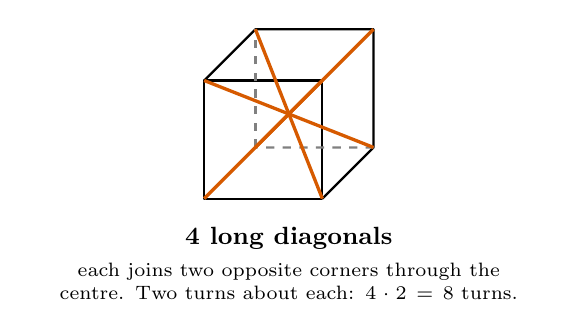
\begin{tikzpicture}[scale=0.5,line join=round]
  \draw[thick] (0,0)--(3,0)--(3,3)--(0,3)--cycle; \draw[thick] (3,0)--(4.3,1.3)--(4.3,4.3)--(3,3); \draw[thick] (0,3)--(1.3,4.3)--(4.3,4.3);
  \draw[thick,dashed,gray] (0,0)--(1.3,1.3)--(4.3,1.3); \draw[thick,dashed,gray] (1.3,1.3)--(1.3,4.3);
  \draw[very thick,mkc] (0,0)--(4.3,4.3);
  \draw[very thick,mkc] (3,0)--(1.3,4.3);
  \draw[very thick,mkc] (3,3)--(1.3,1.3);
  \draw[very thick,mkc] (0,3)--(4.3,1.3);
  \node[font=\small\bfseries] at (2.15,-1.0) {4 long diagonals};
  \node[font=\scriptsize,align=center,text width=6.4cm] at (2.15,-2.1) {each joins two opposite corners through the centre. Two turns about each: $4\cdot2=8$ turns.};
\end{tikzpicture}
\end{minipage}\par\vspace{4pt}
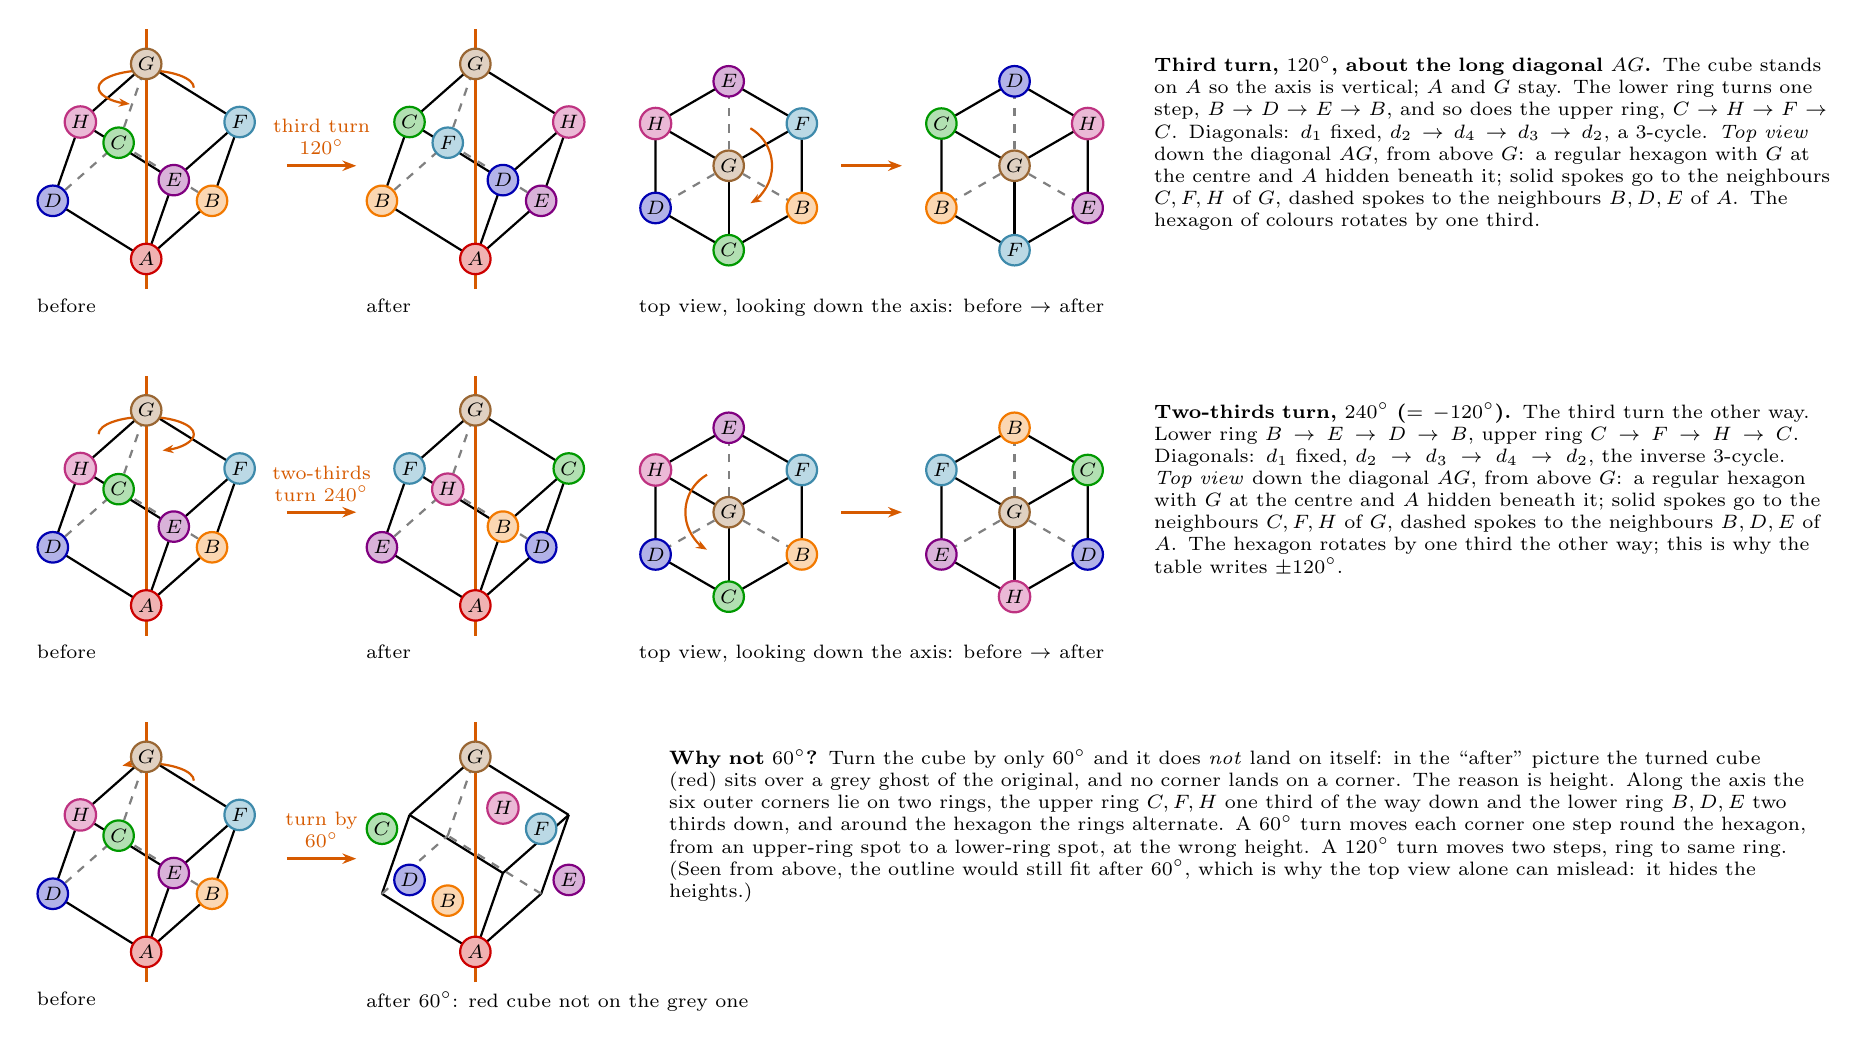
\begin{tikzpicture}[scale=0.55,line join=round]
\begin{scope}[shift={(0,0)}]
  \draw[thick] (2.15,-0.002)--(3.67,1.34);
  \draw[thick] (2.15,-0.002)--(-0.007,1.34);
  \draw[thick] (2.15,-0.002)--(2.787,1.818);
  \draw[thick] (3.67,1.34)--(4.307,3.16);
  \draw[thick] (-0.007,1.34)--(0.63,3.16);
  \draw[thick] (2.787,1.818)--(4.307,3.16);
  \draw[thick] (2.787,1.818)--(0.63,3.16);
  \draw[thick] (4.307,3.16)--(2.15,4.502);
  \draw[thick] (0.63,3.16)--(2.15,4.502);
  \draw[thick,dashed,gray] (3.67,1.34)--(1.513,2.682);
  \draw[thick,dashed,gray] (-0.007,1.34)--(1.513,2.682);
  \draw[thick,dashed,gray] (1.513,2.682)--(2.15,4.502);
  \draw[very thick,mkc] (2.15,-0.7)--(2.15,5.3);
  \draw[-{Stealth[length=4pt]},mkc,thick] (3.25,3.952) arc (0:250:1.1 and 0.4);
  \node[font=\scriptsize\bfseries,circle,inner sep=1pt,minimum size=11pt,fill=red!80!black!30,draw=red!80!black,thick,text=black] at (2.15,-0.002) {$A$};
  \node[font=\scriptsize\bfseries,circle,inner sep=1pt,minimum size=11pt,fill=orange!95!black!30,draw=orange!95!black,thick,text=black] at (3.67,1.34) {$B$};
  \node[font=\scriptsize\bfseries,circle,inner sep=1pt,minimum size=11pt,fill=green!60!black!30,draw=green!60!black,thick,text=black] at (1.513,2.682) {$C$};
  \node[font=\scriptsize\bfseries,circle,inner sep=1pt,minimum size=11pt,fill=blue!70!black!30,draw=blue!70!black,thick,text=black] at (-0.007,1.34) {$D$};
  \node[font=\scriptsize\bfseries,circle,inner sep=1pt,minimum size=11pt,fill=violet!30,draw=violet,thick,text=black] at (2.787,1.818) {$E$};
  \node[font=\scriptsize\bfseries,circle,inner sep=1pt,minimum size=11pt,fill=cyan!65!black!30,draw=cyan!65!black,thick,text=black] at (4.307,3.16) {$F$};
  \node[font=\scriptsize\bfseries,circle,inner sep=1pt,minimum size=11pt,fill=brown!80!black!30,draw=brown!80!black,thick,text=black] at (2.15,4.502) {$G$};
  \node[font=\scriptsize\bfseries,circle,inner sep=1pt,minimum size=11pt,fill=magenta!75!black!30,draw=magenta!75!black,thick,text=black] at (0.63,3.16) {$H$};
\end{scope}
  \draw[-{Stealth[length=5pt]},very thick,mkc] (5.4,2.15) -- node[above,font=\scriptsize,mkc,align=center] {third turn\\$120^\circ$} (7.0,2.15);
\begin{scope}[shift={(7.6,0)}]
  \draw[thick] (2.15,-0.002)--(3.67,1.34);
  \draw[thick] (2.15,-0.002)--(-0.007,1.34);
  \draw[thick] (2.15,-0.002)--(2.787,1.818);
  \draw[thick] (3.67,1.34)--(4.307,3.16);
  \draw[thick] (-0.007,1.34)--(0.63,3.16);
  \draw[thick] (2.787,1.818)--(4.307,3.16);
  \draw[thick] (2.787,1.818)--(0.63,3.16);
  \draw[thick] (4.307,3.16)--(2.15,4.502);
  \draw[thick] (0.63,3.16)--(2.15,4.502);
  \draw[thick,dashed,gray] (3.67,1.34)--(1.513,2.682);
  \draw[thick,dashed,gray] (-0.007,1.34)--(1.513,2.682);
  \draw[thick,dashed,gray] (1.513,2.682)--(2.15,4.502);
  \draw[very thick,mkc] (2.15,-0.7)--(2.15,5.3);
  \node[font=\scriptsize\bfseries,circle,inner sep=1pt,minimum size=11pt,fill=red!80!black!30,draw=red!80!black,thick,text=black] at (2.15,-0.002) {$A$};
  \node[font=\scriptsize\bfseries,circle,inner sep=1pt,minimum size=11pt,fill=orange!95!black!30,draw=orange!95!black,thick,text=black] at (-0.007,1.34) {$B$};
  \node[font=\scriptsize\bfseries,circle,inner sep=1pt,minimum size=11pt,fill=green!60!black!30,draw=green!60!black,thick,text=black] at (0.63,3.16) {$C$};
  \node[font=\scriptsize\bfseries,circle,inner sep=1pt,minimum size=11pt,fill=blue!70!black!30,draw=blue!70!black,thick,text=black] at (2.787,1.818) {$D$};
  \node[font=\scriptsize\bfseries,circle,inner sep=1pt,minimum size=11pt,fill=violet!30,draw=violet,thick,text=black] at (3.67,1.34) {$E$};
  \node[font=\scriptsize\bfseries,circle,inner sep=1pt,minimum size=11pt,fill=cyan!65!black!30,draw=cyan!65!black,thick,text=black] at (1.513,2.682) {$F$};
  \node[font=\scriptsize\bfseries,circle,inner sep=1pt,minimum size=11pt,fill=brown!80!black!30,draw=brown!80!black,thick,text=black] at (2.15,4.502) {$G$};
  \node[font=\scriptsize\bfseries,circle,inner sep=1pt,minimum size=11pt,fill=magenta!75!black!30,draw=magenta!75!black,thick,text=black] at (4.307,3.16) {$H$};
\end{scope}
  \node[font=\scriptsize,anchor=north west] at (-0.6,-0.7) {before};
  \node[font=\scriptsize,anchor=north west] at (7.0,-0.7) {after};
\begin{scope}[shift={(15.6,2.15)}]
  \draw[thick] (30:1.95)--(90:1.95)--(150:1.95)--(210:1.95)--(270:1.95)--(330:1.95)--cycle;
  \draw[thick] (0,0)--(270:1.95);
  \draw[thick] (0,0)--(30:1.95);
  \draw[thick] (0,0)--(150:1.95);
  \draw[thick,dashed,gray] (0,0)--(330:1.95);
  \draw[thick,dashed,gray] (0,0)--(210:1.95);
  \draw[thick,dashed,gray] (0,0)--(90:1.95);
  \fill[mkc] (0,0) circle (2.2pt);
  \draw[-{Stealth[length=4pt]},mkc,thick] (60:1.0) arc (60:-60:1.0);
  \node[font=\scriptsize\bfseries,circle,inner sep=1pt,minimum size=11pt,fill=cyan!65!black!30,draw=cyan!65!black,thick,text=black] at (1.689,0.975) {$F$};
  \node[font=\scriptsize\bfseries,circle,inner sep=1pt,minimum size=11pt,fill=violet!30,draw=violet,thick,text=black] at (0.0,1.95) {$E$};
  \node[font=\scriptsize\bfseries,circle,inner sep=1pt,minimum size=11pt,fill=magenta!75!black!30,draw=magenta!75!black,thick,text=black] at (-1.689,0.975) {$H$};
  \node[font=\scriptsize\bfseries,circle,inner sep=1pt,minimum size=11pt,fill=blue!70!black!30,draw=blue!70!black,thick,text=black] at (-1.689,-0.975) {$D$};
  \node[font=\scriptsize\bfseries,circle,inner sep=1pt,minimum size=11pt,fill=green!60!black!30,draw=green!60!black,thick,text=black] at (-0.0,-1.95) {$C$};
  \node[font=\scriptsize\bfseries,circle,inner sep=1pt,minimum size=11pt,fill=orange!95!black!30,draw=orange!95!black,thick,text=black] at (1.689,-0.975) {$B$};
  \node[font=\scriptsize\bfseries,circle,inner sep=1pt,minimum size=11pt,fill=brown!80!black!30,draw=brown!80!black,thick,text=black] at (0,0) {$G$};
\end{scope}
  \draw[-{Stealth[length=5pt]},very thick,mkc] (18.2,2.15) -- (19.6,2.15);
\begin{scope}[shift={(22.2,2.15)}]
  \draw[thick] (30:1.95)--(90:1.95)--(150:1.95)--(210:1.95)--(270:1.95)--(330:1.95)--cycle;
  \draw[thick] (0,0)--(270:1.95);
  \draw[thick] (0,0)--(30:1.95);
  \draw[thick] (0,0)--(150:1.95);
  \draw[thick,dashed,gray] (0,0)--(330:1.95);
  \draw[thick,dashed,gray] (0,0)--(210:1.95);
  \draw[thick,dashed,gray] (0,0)--(90:1.95);
  \fill[mkc] (0,0) circle (2.2pt);
  \node[font=\scriptsize\bfseries,circle,inner sep=1pt,minimum size=11pt,fill=magenta!75!black!30,draw=magenta!75!black,thick,text=black] at (1.689,0.975) {$H$};
  \node[font=\scriptsize\bfseries,circle,inner sep=1pt,minimum size=11pt,fill=blue!70!black!30,draw=blue!70!black,thick,text=black] at (0.0,1.95) {$D$};
  \node[font=\scriptsize\bfseries,circle,inner sep=1pt,minimum size=11pt,fill=green!60!black!30,draw=green!60!black,thick,text=black] at (-1.689,0.975) {$C$};
  \node[font=\scriptsize\bfseries,circle,inner sep=1pt,minimum size=11pt,fill=orange!95!black!30,draw=orange!95!black,thick,text=black] at (-1.689,-0.975) {$B$};
  \node[font=\scriptsize\bfseries,circle,inner sep=1pt,minimum size=11pt,fill=cyan!65!black!30,draw=cyan!65!black,thick,text=black] at (-0.0,-1.95) {$F$};
  \node[font=\scriptsize\bfseries,circle,inner sep=1pt,minimum size=11pt,fill=violet!30,draw=violet,thick,text=black] at (1.689,-0.975) {$E$};
  \node[font=\scriptsize\bfseries,circle,inner sep=1pt,minimum size=11pt,fill=brown!80!black!30,draw=brown!80!black,thick,text=black] at (0,0) {$G$};
\end{scope}
  \node[font=\scriptsize,anchor=north] at (18.9,-0.7) {top view, looking down the axis: before $\to$ after};
  \node[font=\scriptsize,align=left,text width=8.6cm,anchor=north west] at (25.2,4.9) {\textbf{Third turn, $120^\circ$, about the long diagonal $AG$.} The cube stands on $A$ so the axis is vertical; $A$ and $G$ stay. The lower ring turns one step, $B\to D\to E\to B$, and so does the upper ring, $C\to H\to F\to C$. Diagonals: $d_1$ fixed, $d_2\to d_4\to d_3\to d_2$, a 3-cycle. \emph{Top view} down the diagonal $AG$, from above $G$: a regular hexagon with $G$ at the centre and $A$ hidden beneath it; solid spokes go to the neighbours $C,F,H$ of $G$, dashed spokes to the neighbours $B,D,E$ of $A$. The hexagon of colours rotates by one third.};
\begin{scope}[shift={(0,-8.0)}]
  \draw[thick] (2.15,-0.002)--(3.67,1.34);
  \draw[thick] (2.15,-0.002)--(-0.007,1.34);
  \draw[thick] (2.15,-0.002)--(2.787,1.818);
  \draw[thick] (3.67,1.34)--(4.307,3.16);
  \draw[thick] (-0.007,1.34)--(0.63,3.16);
  \draw[thick] (2.787,1.818)--(4.307,3.16);
  \draw[thick] (2.787,1.818)--(0.63,3.16);
  \draw[thick] (4.307,3.16)--(2.15,4.502);
  \draw[thick] (0.63,3.16)--(2.15,4.502);
  \draw[thick,dashed,gray] (3.67,1.34)--(1.513,2.682);
  \draw[thick,dashed,gray] (-0.007,1.34)--(1.513,2.682);
  \draw[thick,dashed,gray] (1.513,2.682)--(2.15,4.502);
  \draw[very thick,mkc] (2.15,-0.7)--(2.15,5.3);
  \draw[-{Stealth[length=4pt]},mkc,thick] (1.05,3.952) arc (180:-70:1.1 and 0.4);
  \node[font=\scriptsize\bfseries,circle,inner sep=1pt,minimum size=11pt,fill=red!80!black!30,draw=red!80!black,thick,text=black] at (2.15,-0.002) {$A$};
  \node[font=\scriptsize\bfseries,circle,inner sep=1pt,minimum size=11pt,fill=orange!95!black!30,draw=orange!95!black,thick,text=black] at (3.67,1.34) {$B$};
  \node[font=\scriptsize\bfseries,circle,inner sep=1pt,minimum size=11pt,fill=green!60!black!30,draw=green!60!black,thick,text=black] at (1.513,2.682) {$C$};
  \node[font=\scriptsize\bfseries,circle,inner sep=1pt,minimum size=11pt,fill=blue!70!black!30,draw=blue!70!black,thick,text=black] at (-0.007,1.34) {$D$};
  \node[font=\scriptsize\bfseries,circle,inner sep=1pt,minimum size=11pt,fill=violet!30,draw=violet,thick,text=black] at (2.787,1.818) {$E$};
  \node[font=\scriptsize\bfseries,circle,inner sep=1pt,minimum size=11pt,fill=cyan!65!black!30,draw=cyan!65!black,thick,text=black] at (4.307,3.16) {$F$};
  \node[font=\scriptsize\bfseries,circle,inner sep=1pt,minimum size=11pt,fill=brown!80!black!30,draw=brown!80!black,thick,text=black] at (2.15,4.502) {$G$};
  \node[font=\scriptsize\bfseries,circle,inner sep=1pt,minimum size=11pt,fill=magenta!75!black!30,draw=magenta!75!black,thick,text=black] at (0.63,3.16) {$H$};
\end{scope}
  \draw[-{Stealth[length=5pt]},very thick,mkc] (5.4,-5.85) -- node[above,font=\scriptsize,mkc,align=center] {two-thirds\\turn $240^\circ$} (7.0,-5.85);
\begin{scope}[shift={(7.6,-8.0)}]
  \draw[thick] (2.15,-0.002)--(3.67,1.34);
  \draw[thick] (2.15,-0.002)--(-0.007,1.34);
  \draw[thick] (2.15,-0.002)--(2.787,1.818);
  \draw[thick] (3.67,1.34)--(4.307,3.16);
  \draw[thick] (-0.007,1.34)--(0.63,3.16);
  \draw[thick] (2.787,1.818)--(4.307,3.16);
  \draw[thick] (2.787,1.818)--(0.63,3.16);
  \draw[thick] (4.307,3.16)--(2.15,4.502);
  \draw[thick] (0.63,3.16)--(2.15,4.502);
  \draw[thick,dashed,gray] (3.67,1.34)--(1.513,2.682);
  \draw[thick,dashed,gray] (-0.007,1.34)--(1.513,2.682);
  \draw[thick,dashed,gray] (1.513,2.682)--(2.15,4.502);
  \draw[very thick,mkc] (2.15,-0.7)--(2.15,5.3);
  \node[font=\scriptsize\bfseries,circle,inner sep=1pt,minimum size=11pt,fill=red!80!black!30,draw=red!80!black,thick,text=black] at (2.15,-0.002) {$A$};
  \node[font=\scriptsize\bfseries,circle,inner sep=1pt,minimum size=11pt,fill=orange!95!black!30,draw=orange!95!black,thick,text=black] at (2.787,1.818) {$B$};
  \node[font=\scriptsize\bfseries,circle,inner sep=1pt,minimum size=11pt,fill=green!60!black!30,draw=green!60!black,thick,text=black] at (4.307,3.16) {$C$};
  \node[font=\scriptsize\bfseries,circle,inner sep=1pt,minimum size=11pt,fill=blue!70!black!30,draw=blue!70!black,thick,text=black] at (3.67,1.34) {$D$};
  \node[font=\scriptsize\bfseries,circle,inner sep=1pt,minimum size=11pt,fill=violet!30,draw=violet,thick,text=black] at (-0.007,1.34) {$E$};
  \node[font=\scriptsize\bfseries,circle,inner sep=1pt,minimum size=11pt,fill=cyan!65!black!30,draw=cyan!65!black,thick,text=black] at (0.63,3.16) {$F$};
  \node[font=\scriptsize\bfseries,circle,inner sep=1pt,minimum size=11pt,fill=brown!80!black!30,draw=brown!80!black,thick,text=black] at (2.15,4.502) {$G$};
  \node[font=\scriptsize\bfseries,circle,inner sep=1pt,minimum size=11pt,fill=magenta!75!black!30,draw=magenta!75!black,thick,text=black] at (1.513,2.682) {$H$};
\end{scope}
  \node[font=\scriptsize,anchor=north west] at (-0.6,-8.7) {before};
  \node[font=\scriptsize,anchor=north west] at (7.0,-8.7) {after};
\begin{scope}[shift={(15.6,-5.85)}]
  \draw[thick] (30:1.95)--(90:1.95)--(150:1.95)--(210:1.95)--(270:1.95)--(330:1.95)--cycle;
  \draw[thick] (0,0)--(270:1.95);
  \draw[thick] (0,0)--(30:1.95);
  \draw[thick] (0,0)--(150:1.95);
  \draw[thick,dashed,gray] (0,0)--(330:1.95);
  \draw[thick,dashed,gray] (0,0)--(210:1.95);
  \draw[thick,dashed,gray] (0,0)--(90:1.95);
  \fill[mkc] (0,0) circle (2.2pt);
  \draw[-{Stealth[length=4pt]},mkc,thick] (120:1.0) arc (120:240:1.0);
  \node[font=\scriptsize\bfseries,circle,inner sep=1pt,minimum size=11pt,fill=cyan!65!black!30,draw=cyan!65!black,thick,text=black] at (1.689,0.975) {$F$};
  \node[font=\scriptsize\bfseries,circle,inner sep=1pt,minimum size=11pt,fill=violet!30,draw=violet,thick,text=black] at (0.0,1.95) {$E$};
  \node[font=\scriptsize\bfseries,circle,inner sep=1pt,minimum size=11pt,fill=magenta!75!black!30,draw=magenta!75!black,thick,text=black] at (-1.689,0.975) {$H$};
  \node[font=\scriptsize\bfseries,circle,inner sep=1pt,minimum size=11pt,fill=blue!70!black!30,draw=blue!70!black,thick,text=black] at (-1.689,-0.975) {$D$};
  \node[font=\scriptsize\bfseries,circle,inner sep=1pt,minimum size=11pt,fill=green!60!black!30,draw=green!60!black,thick,text=black] at (-0.0,-1.95) {$C$};
  \node[font=\scriptsize\bfseries,circle,inner sep=1pt,minimum size=11pt,fill=orange!95!black!30,draw=orange!95!black,thick,text=black] at (1.689,-0.975) {$B$};
  \node[font=\scriptsize\bfseries,circle,inner sep=1pt,minimum size=11pt,fill=brown!80!black!30,draw=brown!80!black,thick,text=black] at (0,0) {$G$};
\end{scope}
  \draw[-{Stealth[length=5pt]},very thick,mkc] (18.2,-5.85) -- (19.6,-5.85);
\begin{scope}[shift={(22.2,-5.85)}]
  \draw[thick] (30:1.95)--(90:1.95)--(150:1.95)--(210:1.95)--(270:1.95)--(330:1.95)--cycle;
  \draw[thick] (0,0)--(270:1.95);
  \draw[thick] (0,0)--(30:1.95);
  \draw[thick] (0,0)--(150:1.95);
  \draw[thick,dashed,gray] (0,0)--(330:1.95);
  \draw[thick,dashed,gray] (0,0)--(210:1.95);
  \draw[thick,dashed,gray] (0,0)--(90:1.95);
  \fill[mkc] (0,0) circle (2.2pt);
  \node[font=\scriptsize\bfseries,circle,inner sep=1pt,minimum size=11pt,fill=green!60!black!30,draw=green!60!black,thick,text=black] at (1.689,0.975) {$C$};
  \node[font=\scriptsize\bfseries,circle,inner sep=1pt,minimum size=11pt,fill=orange!95!black!30,draw=orange!95!black,thick,text=black] at (0.0,1.95) {$B$};
  \node[font=\scriptsize\bfseries,circle,inner sep=1pt,minimum size=11pt,fill=cyan!65!black!30,draw=cyan!65!black,thick,text=black] at (-1.689,0.975) {$F$};
  \node[font=\scriptsize\bfseries,circle,inner sep=1pt,minimum size=11pt,fill=violet!30,draw=violet,thick,text=black] at (-1.689,-0.975) {$E$};
  \node[font=\scriptsize\bfseries,circle,inner sep=1pt,minimum size=11pt,fill=magenta!75!black!30,draw=magenta!75!black,thick,text=black] at (-0.0,-1.95) {$H$};
  \node[font=\scriptsize\bfseries,circle,inner sep=1pt,minimum size=11pt,fill=blue!70!black!30,draw=blue!70!black,thick,text=black] at (1.689,-0.975) {$D$};
  \node[font=\scriptsize\bfseries,circle,inner sep=1pt,minimum size=11pt,fill=brown!80!black!30,draw=brown!80!black,thick,text=black] at (0,0) {$G$};
\end{scope}
  \node[font=\scriptsize,anchor=north] at (18.9,-8.7) {top view, looking down the axis: before $\to$ after};
  \node[font=\scriptsize,align=left,text width=8.6cm,anchor=north west] at (25.2,-3.1) {\textbf{Two-thirds turn, $240^\circ$ ($=-120^\circ$).} The third turn the other way. Lower ring $B\to E\to D\to B$, upper ring $C\to F\to H\to C$. Diagonals: $d_1$ fixed, $d_2\to d_3\to d_4\to d_2$, the inverse 3-cycle. \emph{Top view} down the diagonal $AG$, from above $G$: a regular hexagon with $G$ at the centre and $A$ hidden beneath it; solid spokes go to the neighbours $C,F,H$ of $G$, dashed spokes to the neighbours $B,D,E$ of $A$. The hexagon rotates by one third the other way; this is why the table writes $\pm120^\circ$.};
\begin{scope}[shift={(0,-16.0)}]
  \draw[thick] (2.15,-0.002)--(3.67,1.34);
  \draw[thick] (2.15,-0.002)--(-0.007,1.34);
  \draw[thick] (2.15,-0.002)--(2.787,1.818);
  \draw[thick] (3.67,1.34)--(4.307,3.16);
  \draw[thick] (-0.007,1.34)--(0.63,3.16);
  \draw[thick] (2.787,1.818)--(4.307,3.16);
  \draw[thick] (2.787,1.818)--(0.63,3.16);
  \draw[thick] (4.307,3.16)--(2.15,4.502);
  \draw[thick] (0.63,3.16)--(2.15,4.502);
  \draw[thick,dashed,gray] (3.67,1.34)--(1.513,2.682);
  \draw[thick,dashed,gray] (-0.007,1.34)--(1.513,2.682);
  \draw[thick,dashed,gray] (1.513,2.682)--(2.15,4.502);
  \draw[very thick,mkc] (2.15,-0.7)--(2.15,5.3);
  \draw[-{Stealth[length=4pt]},mkc,thick] (3.25,3.952) arc (0:120:1.1 and 0.4);
  \node[font=\scriptsize\bfseries,circle,inner sep=1pt,minimum size=11pt,fill=red!80!black!30,draw=red!80!black,thick,text=black] at (2.15,-0.002) {$A$};
  \node[font=\scriptsize\bfseries,circle,inner sep=1pt,minimum size=11pt,fill=orange!95!black!30,draw=orange!95!black,thick,text=black] at (3.67,1.34) {$B$};
  \node[font=\scriptsize\bfseries,circle,inner sep=1pt,minimum size=11pt,fill=green!60!black!30,draw=green!60!black,thick,text=black] at (1.513,2.682) {$C$};
  \node[font=\scriptsize\bfseries,circle,inner sep=1pt,minimum size=11pt,fill=blue!70!black!30,draw=blue!70!black,thick,text=black] at (-0.007,1.34) {$D$};
  \node[font=\scriptsize\bfseries,circle,inner sep=1pt,minimum size=11pt,fill=violet!30,draw=violet,thick,text=black] at (2.787,1.818) {$E$};
  \node[font=\scriptsize\bfseries,circle,inner sep=1pt,minimum size=11pt,fill=cyan!65!black!30,draw=cyan!65!black,thick,text=black] at (4.307,3.16) {$F$};
  \node[font=\scriptsize\bfseries,circle,inner sep=1pt,minimum size=11pt,fill=brown!80!black!30,draw=brown!80!black,thick,text=black] at (2.15,4.502) {$G$};
  \node[font=\scriptsize\bfseries,circle,inner sep=1pt,minimum size=11pt,fill=magenta!75!black!30,draw=magenta!75!black,thick,text=black] at (0.63,3.16) {$H$};
\end{scope}
  \draw[-{Stealth[length=5pt]},very thick,mkc] (5.4,-13.85) -- node[above,font=\scriptsize,mkc,align=center] {turn by\\$60^\circ$} (7.0,-13.85);
\begin{scope}[shift={(7.6,-16.0)}]
  \draw[thin,gray!60] (2.15,-0.002)--(3.67,1.34);
  \draw[thin,gray!60] (2.15,-0.002)--(-0.007,1.34);
  \draw[thin,gray!60] (2.15,-0.002)--(2.787,1.818);
  \draw[thin,gray!60] (3.67,1.34)--(4.307,3.16);
  \draw[thin,gray!60] (-0.007,1.34)--(0.63,3.16);
  \draw[thin,gray!60] (2.787,1.818)--(4.307,3.16);
  \draw[thin,gray!60] (2.787,1.818)--(0.63,3.16);
  \draw[thin,gray!60] (4.307,3.16)--(2.15,4.502);
  \draw[thin,gray!60] (0.63,3.16)--(2.15,4.502);
  \draw[thin,gray!40,dashed] (3.67,1.34)--(1.513,2.682);
  \draw[thin,gray!40,dashed] (-0.007,1.34)--(1.513,2.682);
  \draw[thin,gray!40,dashed] (1.513,2.682)--(2.15,4.502);
\end{scope}
\begin{scope}[shift={(7.6,-16.0)}]
  \draw[thick] (2.15,-0.002)--(3.67,1.34);
  \draw[thick] (2.15,-0.002)--(-0.007,1.34);
  \draw[thick] (2.15,-0.002)--(2.787,1.818);
  \draw[thick] (3.67,1.34)--(4.307,3.16);
  \draw[thick] (-0.007,1.34)--(0.63,3.16);
  \draw[thick] (2.787,1.818)--(4.307,3.16);
  \draw[thick] (2.787,1.818)--(0.63,3.16);
  \draw[thick] (4.307,3.16)--(2.15,4.502);
  \draw[thick] (0.63,3.16)--(2.15,4.502);
  \draw[thick,dashed,gray] (3.67,1.34)--(1.513,2.682);
  \draw[thick,dashed,gray] (-0.007,1.34)--(1.513,2.682);
  \draw[thick,dashed,gray] (1.513,2.682)--(2.15,4.502);
  \draw[very thick,mkc] (2.15,-0.7)--(2.15,5.3);
  \node[font=\scriptsize\bfseries,circle,inner sep=1pt,minimum size=11pt,fill=red!80!black!30,draw=red!80!black,thick,text=black] at (2.15,-0.002) {$A$};
  \node[font=\scriptsize\bfseries,circle,inner sep=1pt,minimum size=11pt,fill=orange!95!black!30,draw=orange!95!black,thick,text=black] at (1.513,1.181) {$B$};
  \node[font=\scriptsize\bfseries,circle,inner sep=1pt,minimum size=11pt,fill=green!60!black!30,draw=green!60!black,thick,text=black] at (-0.007,2.841) {$C$};
  \node[font=\scriptsize\bfseries,circle,inner sep=1pt,minimum size=11pt,fill=blue!70!black!30,draw=blue!70!black,thick,text=black] at (0.63,1.659) {$D$};
  \node[font=\scriptsize\bfseries,circle,inner sep=1pt,minimum size=11pt,fill=violet!30,draw=violet,thick,text=black] at (4.307,1.659) {$E$};
  \node[font=\scriptsize\bfseries,circle,inner sep=1pt,minimum size=11pt,fill=cyan!65!black!30,draw=cyan!65!black,thick,text=black] at (3.67,2.841) {$F$};
  \node[font=\scriptsize\bfseries,circle,inner sep=1pt,minimum size=11pt,fill=brown!80!black!30,draw=brown!80!black,thick,text=black] at (2.15,4.502) {$G$};
  \node[font=\scriptsize\bfseries,circle,inner sep=1pt,minimum size=11pt,fill=magenta!75!black!30,draw=magenta!75!black,thick,text=black] at (2.787,3.319) {$H$};
\end{scope}
  \node[font=\scriptsize,anchor=north west] at (-0.6,-16.7) {before};
  \node[font=\scriptsize,anchor=north west] at (7.0,-16.7) {after $60^\circ$: red cube not on the grey one};
  \node[font=\scriptsize,align=left,text width=14.5cm,anchor=north west] at (14.0,-11.1) {\textbf{Why not $60^\circ$?} Turn the cube by only $60^\circ$ and it does \emph{not} land on itself: in the ``after'' picture the turned cube (red) sits over a grey ghost of the original, and no corner lands on a corner. The reason is height. Along the axis the six outer corners lie on two rings, the upper ring $C,F,H$ one third of the way down and the lower ring $B,D,E$ two thirds down, and around the hexagon the rings alternate. A $60^\circ$ turn moves each corner one step round the hexagon, from an upper-ring spot to a lower-ring spot, at the wrong height. A $120^\circ$ turn moves two steps, ring to same ring. (Seen from above, the outline would still fit after $60^\circ$, which is why the top view alone can mislead: it hides the heights.)};
\end{tikzpicture}
\par\vspace{6pt}
\begin{minipage}[t]{744pt}\vspace{0pt}\raggedright
\begin{pitfall}\footnotesize
Two other ways to see that only $120^\circ$ and $240^\circ$ work: looking straight down the axis, the three edges meeting at the near corner form a Y inside the hexagon, and the Y has only 3-fold symmetry; and a rotation about the axis must map the three-corner upper ring to itself, so only multiples of $360^\circ/3$ are possible. A $60^\circ$ turn \emph{combined with} a reflection in the plane halfway up the axis does map the cube to itself, but that is a mirror-type symmetry you cannot perform by turning the cube, so it is not among the 24 rotations; with mirrors allowed the group has 48 elements (Interlude B2).
\end{pitfall}
\end{minipage}
\end{minipage}
}

% ================================================================ INTERLUDE A4 (edge axis)
\interlude{A4. Edge axes: one turn about each}{
\begin{minipage}[t]{744pt}\vspace{0pt}
\begin{minipage}[t]{530pt}\vspace{0pt}\small
An edge axis joins the midpoints of two opposite edges. The cube is drawn standing on that edge so the axis is vertical. Same colour code, same three views. The cube on the right shows all six edge axes with the twelve edge midpoints dotted; the row uses the axis through the midpoints of $AB$ and $GH$.
\end{minipage}\hfill
\begin{minipage}[t]{200pt}\vspace{0pt}\centering
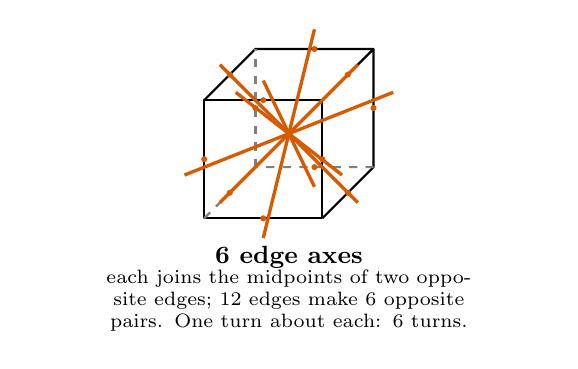
\begin{tikzpicture}[scale=0.5,line join=round]
  \draw[thick] (0,0)--(3,0)--(3,3)--(0,3)--cycle; \draw[thick] (3,0)--(4.3,1.3)--(4.3,4.3)--(3,3); \draw[thick] (0,3)--(1.3,4.3)--(4.3,4.3);
  \draw[thick,dashed,gray] (0,0)--(1.3,1.3)--(4.3,1.3); \draw[thick,dashed,gray] (1.3,1.3)--(1.3,4.3);
  \draw[very thick,mkc] (1.5,-0.5)--(2.8,4.8);
  \draw[very thick,mkc] (3.5,1.1)--(0.8,3.2);
  \draw[very thick,mkc] (1.5,3.5)--(2.8,0.8);
  \draw[very thick,mkc] (-0.5,1.1)--(4.8,3.2);
  \draw[very thick,mkc] (0.4,0.4)--(3.9,3.9);
  \draw[very thick,mkc] (3.9,0.4)--(0.4,3.9);
  \fill[mkc] (1.5,0) circle (2.2pt);
  \fill[mkc] (2.8,4.3) circle (2.2pt);
  \fill[mkc] (3,1.5) circle (2.2pt);
  \fill[mkc] (1.3,2.8) circle (2.2pt);
  \fill[mkc] (1.5,3) circle (2.2pt);
  \fill[mkc] (2.8,1.3) circle (2.2pt);
  \fill[mkc] (0,1.5) circle (2.2pt);
  \fill[mkc] (4.3,2.8) circle (2.2pt);
  \fill[mkc] (0.65,0.65) circle (2.2pt);
  \fill[mkc] (3.65,3.65) circle (2.2pt);
  \fill[mkc] (3.65,0.65) circle (2.2pt);
  \fill[mkc] (0.65,3.65) circle (2.2pt);
  \node[font=\small\bfseries] at (2.15,-1.0) {6 edge axes};
  \node[font=\scriptsize,align=center,text width=6.4cm] at (2.15,-2.1) {each joins the midpoints of two opposite edges; 12 edges make 6 opposite pairs. One turn about each: $6$ turns.};
\end{tikzpicture}
\end{minipage}\par\vspace{4pt}
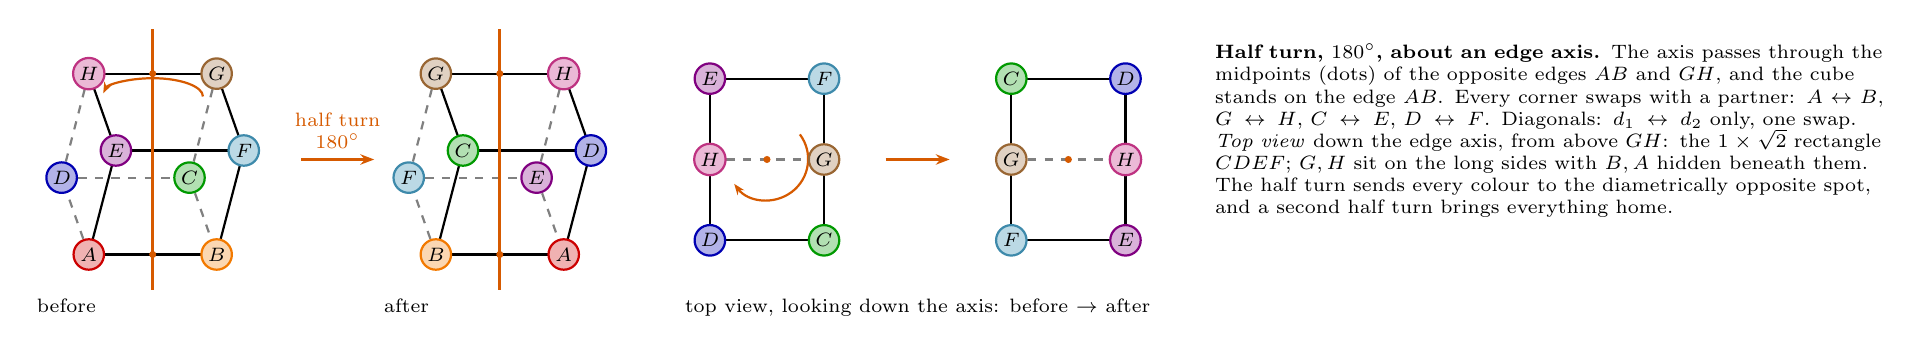
\begin{tikzpicture}[scale=0.58,line join=round]
\begin{scope}[shift={(0,0)}]
  \draw[thick] (0.75,0.07)--(3.55,0.07);
  \draw[thick] (0.75,0.07)--(1.344,2.347);
  \draw[thick] (3.55,0.07)--(4.144,2.347);
  \draw[thick] (1.344,2.347)--(4.144,2.347);
  \draw[thick] (1.344,2.347)--(0.75,4.03);
  \draw[thick] (4.144,2.347)--(3.55,4.03);
  \draw[thick] (0.75,4.03)--(3.55,4.03);
  \draw[thick,dashed,gray] (0.75,0.07)--(0.156,1.753);
  \draw[thick,dashed,gray] (0.156,1.753)--(0.75,4.03);
  \draw[thick,dashed,gray] (0.156,1.753)--(2.956,1.753);
  \draw[thick,dashed,gray] (2.956,1.753)--(3.55,0.07);
  \draw[thick,dashed,gray] (2.956,1.753)--(3.55,4.03);
  \draw[very thick,mkc] (2.15,-0.7)--(2.15,5.0);
  \draw[-{Stealth[length=4pt]},mkc,thick] (3.25,3.5300000000000002) arc (0:170:1.1 and 0.4);
  \fill[mkc] (2.15,0.07) circle (2.2pt); \fill[mkc] (2.15,4.03) circle (2.2pt);
  \node[font=\scriptsize\bfseries,circle,inner sep=1pt,minimum size=11pt,fill=red!80!black!30,draw=red!80!black,thick,text=black] at (0.75,0.07) {$A$};
  \node[font=\scriptsize\bfseries,circle,inner sep=1pt,minimum size=11pt,fill=orange!95!black!30,draw=orange!95!black,thick,text=black] at (3.55,0.07) {$B$};
  \node[font=\scriptsize\bfseries,circle,inner sep=1pt,minimum size=11pt,fill=green!60!black!30,draw=green!60!black,thick,text=black] at (2.956,1.753) {$C$};
  \node[font=\scriptsize\bfseries,circle,inner sep=1pt,minimum size=11pt,fill=blue!70!black!30,draw=blue!70!black,thick,text=black] at (0.156,1.753) {$D$};
  \node[font=\scriptsize\bfseries,circle,inner sep=1pt,minimum size=11pt,fill=violet!30,draw=violet,thick,text=black] at (1.344,2.347) {$E$};
  \node[font=\scriptsize\bfseries,circle,inner sep=1pt,minimum size=11pt,fill=cyan!65!black!30,draw=cyan!65!black,thick,text=black] at (4.144,2.347) {$F$};
  \node[font=\scriptsize\bfseries,circle,inner sep=1pt,minimum size=11pt,fill=brown!80!black!30,draw=brown!80!black,thick,text=black] at (3.55,4.03) {$G$};
  \node[font=\scriptsize\bfseries,circle,inner sep=1pt,minimum size=11pt,fill=magenta!75!black!30,draw=magenta!75!black,thick,text=black] at (0.75,4.03) {$H$};
\end{scope}
  \draw[-{Stealth[length=5pt]},very thick,mkc] (5.4,2.15) -- node[above,font=\scriptsize,mkc,align=center] {half turn\\$180^\circ$} (7.0,2.15);
\begin{scope}[shift={(7.6,0)}]
  \draw[thick] (0.75,0.07)--(3.55,0.07);
  \draw[thick] (0.75,0.07)--(1.344,2.347);
  \draw[thick] (3.55,0.07)--(4.144,2.347);
  \draw[thick] (1.344,2.347)--(4.144,2.347);
  \draw[thick] (1.344,2.347)--(0.75,4.03);
  \draw[thick] (4.144,2.347)--(3.55,4.03);
  \draw[thick] (0.75,4.03)--(3.55,4.03);
  \draw[thick,dashed,gray] (0.75,0.07)--(0.156,1.753);
  \draw[thick,dashed,gray] (0.156,1.753)--(0.75,4.03);
  \draw[thick,dashed,gray] (0.156,1.753)--(2.956,1.753);
  \draw[thick,dashed,gray] (2.956,1.753)--(3.55,0.07);
  \draw[thick,dashed,gray] (2.956,1.753)--(3.55,4.03);
  \draw[very thick,mkc] (2.15,-0.7)--(2.15,5.0);
  \fill[mkc] (2.15,0.07) circle (2.2pt); \fill[mkc] (2.15,4.03) circle (2.2pt);
  \node[font=\scriptsize\bfseries,circle,inner sep=1pt,minimum size=11pt,fill=red!80!black!30,draw=red!80!black,thick,text=black] at (3.55,0.07) {$A$};
  \node[font=\scriptsize\bfseries,circle,inner sep=1pt,minimum size=11pt,fill=orange!95!black!30,draw=orange!95!black,thick,text=black] at (0.75,0.07) {$B$};
  \node[font=\scriptsize\bfseries,circle,inner sep=1pt,minimum size=11pt,fill=brown!80!black!30,draw=brown!80!black,thick,text=black] at (0.75,4.03) {$G$};
  \node[font=\scriptsize\bfseries,circle,inner sep=1pt,minimum size=11pt,fill=magenta!75!black!30,draw=magenta!75!black,thick,text=black] at (3.55,4.03) {$H$};
  \node[font=\scriptsize\bfseries,circle,inner sep=1pt,minimum size=11pt,fill=green!60!black!30,draw=green!60!black,thick,text=black] at (1.344,2.347) {$C$};
  \node[font=\scriptsize\bfseries,circle,inner sep=1pt,minimum size=11pt,fill=violet!30,draw=violet,thick,text=black] at (2.956,1.753) {$E$};
  \node[font=\scriptsize\bfseries,circle,inner sep=1pt,minimum size=11pt,fill=blue!70!black!30,draw=blue!70!black,thick,text=black] at (4.144,2.347) {$D$};
  \node[font=\scriptsize\bfseries,circle,inner sep=1pt,minimum size=11pt,fill=cyan!65!black!30,draw=cyan!65!black,thick,text=black] at (0.156,1.753) {$F$};
\end{scope}
  \node[font=\scriptsize,anchor=north west] at (-0.6,-0.7) {before};
  \node[font=\scriptsize,anchor=north west] at (7.0,-0.7) {after};
\begin{scope}[shift={(15.6,2.15)}]
  \draw[thick] (1.25,1.77)--(-1.25,1.77)--(-1.25,-1.77)--(1.25,-1.77)--cycle;
  \draw[thick,dashed,gray] (-1.25,0)--(1.25,0);
  \fill[mkc] (0,0) circle (2.2pt);
  \draw[-{Stealth[length=4pt]},mkc,thick] (0.72,0.55) arc (37:-143:0.9);
  \node[font=\scriptsize\bfseries,circle,inner sep=1pt,minimum size=11pt,fill=green!60!black!30,draw=green!60!black,thick,text=black] at (1.25,-1.77) {$C$};
  \node[font=\scriptsize\bfseries,circle,inner sep=1pt,minimum size=11pt,fill=blue!70!black!30,draw=blue!70!black,thick,text=black] at (-1.25,-1.77) {$D$};
  \node[font=\scriptsize\bfseries,circle,inner sep=1pt,minimum size=11pt,fill=violet!30,draw=violet,thick,text=black] at (-1.25,1.77) {$E$};
  \node[font=\scriptsize\bfseries,circle,inner sep=1pt,minimum size=11pt,fill=cyan!65!black!30,draw=cyan!65!black,thick,text=black] at (1.25,1.77) {$F$};
  \node[font=\scriptsize\bfseries,circle,inner sep=1pt,minimum size=11pt,fill=brown!80!black!30,draw=brown!80!black,thick,text=black] at (1.25,0) {$G$};
  \node[font=\scriptsize\bfseries,circle,inner sep=1pt,minimum size=11pt,fill=magenta!75!black!30,draw=magenta!75!black,thick,text=black] at (-1.25,0) {$H$};
\end{scope}
  \draw[-{Stealth[length=5pt]},very thick,mkc] (18.2,2.15) -- (19.6,2.15);
\begin{scope}[shift={(22.2,2.15)}]
  \draw[thick] (1.25,1.77)--(-1.25,1.77)--(-1.25,-1.77)--(1.25,-1.77)--cycle;
  \draw[thick,dashed,gray] (-1.25,0)--(1.25,0);
  \fill[mkc] (0,0) circle (2.2pt);
  \node[font=\scriptsize\bfseries,circle,inner sep=1pt,minimum size=11pt,fill=violet!30,draw=violet,thick,text=black] at (1.25,-1.77) {$E$};
  \node[font=\scriptsize\bfseries,circle,inner sep=1pt,minimum size=11pt,fill=cyan!65!black!30,draw=cyan!65!black,thick,text=black] at (-1.25,-1.77) {$F$};
  \node[font=\scriptsize\bfseries,circle,inner sep=1pt,minimum size=11pt,fill=green!60!black!30,draw=green!60!black,thick,text=black] at (-1.25,1.77) {$C$};
  \node[font=\scriptsize\bfseries,circle,inner sep=1pt,minimum size=11pt,fill=blue!70!black!30,draw=blue!70!black,thick,text=black] at (1.25,1.77) {$D$};
  \node[font=\scriptsize\bfseries,circle,inner sep=1pt,minimum size=11pt,fill=magenta!75!black!30,draw=magenta!75!black,thick,text=black] at (1.25,0) {$H$};
  \node[font=\scriptsize\bfseries,circle,inner sep=1pt,minimum size=11pt,fill=brown!80!black!30,draw=brown!80!black,thick,text=black] at (-1.25,0) {$G$};
\end{scope}
  \node[font=\scriptsize,anchor=north] at (18.9,-0.7) {top view, looking down the axis: before $\to$ after};
  \node[font=\scriptsize,align=left,text width=8.6cm,anchor=north west] at (25.2,4.9) {\textbf{Half turn, $180^\circ$, about an edge axis.} The axis passes through the midpoints (dots) of the opposite edges $AB$ and $GH$, and the cube stands on the edge $AB$. Every corner swaps with a partner: $A\leftrightarrow B$, $G\leftrightarrow H$, $C\leftrightarrow E$, $D\leftrightarrow F$. Diagonals: $d_1\leftrightarrow d_2$ only, one swap. \emph{Top view} down the edge axis, from above $GH$: the $1\times\sqrt2$ rectangle $CDEF$; $G,H$ sit on the long sides with $B,A$ hidden beneath them. The half turn sends every colour to the diametrically opposite spot, and a second half turn brings everything home.};
\end{tikzpicture}
\end{minipage}
}

% ================================================================ INTERLUDE A5 (reading guide)
\interlude{A5. Putting the three kinds together, and how to read the pictures}{
\begin{minipage}[t]{744pt}\vspace{0pt}
\small
\begin{center}
\begin{tabular}{@{}lccc@{}}
\toprule
kind of axis & how many axes & turns about each & turns in all\\
\midrule
through two opposite face centres & 3 & 3 ($90^\circ,180^\circ,270^\circ$) & 9\\
through two opposite corners (long diagonal) & 4 & 2 ($120^\circ,240^\circ$) & 8\\
through the midpoints of two opposite edges & 6 & 1 ($180^\circ$) & 6\\
\midrule
plus the identity & & & 1\\
total & & & 24\\
\bottomrule
\end{tabular}
\end{center}
\vspace{8pt}
\begin{minipage}[t]{360pt}\vspace{0pt}\raggedright
\begin{why}
How to read a diagonal off a before/after pair: a diagonal is named by its two ends, so look where both ends went. In the quarter turn, $A$ now sits in $B$'s corner and $G$ in $H$'s, so the diagonal $d_1=AG$ now occupies the slot of $BH=d_2$. Likewise $B,H$ have gone to the corners $F,D$, so $d_2$ occupies the slot of $d_4$; and so on round the 4-cycle. In the edge half-turn, $C$ and $E$ have swapped, so the diagonal $CE=d_3$ occupies its own slot, reversed: as a diagonal it is fixed.
\end{why}
\begin{why}
Why $270^\circ$ and $240^\circ$ are listed as ``$-90^\circ$'' and ``$-120^\circ$'': turning by $270^\circ$ one way lands the cube exactly where turning by $90^\circ$ the other way does, so it is the same symmetry, the inverse of the quarter turn, with every corner move reversed. That is why the table writes $\pm90^\circ$ and $\pm120^\circ$ and counts two turns per axis. The half turns are their own inverses, so they come singly.
\end{why}
\end{minipage}\hfill
\begin{minipage}[t]{360pt}\vspace{0pt}\raggedright
\begin{pitfall}
Same kind of turn, different axis, different permutation. The quarter turn drawn is about the top--bottom axis and gives the 4-cycle $(d_1\,d_2\,d_4\,d_3)$; the quarter turn about the front--back axis gives a different 4-cycle. There are 6 quarter turns in all (3 axes, 2 directions) and 6 four-cycles in $S_4$: one each. The same matching holds row by row: 3 half turns and 3 double swaps, 8 third turns and 8 three-cycles, 6 edge turns and 6 single swaps.
\end{pitfall}
\begin{tryit}
Do the $120^\circ$ picture and then the $240^\circ$ picture one after the other, reading the ``after'' of the first as the ``before'' of the second: every colour returns home. One third plus two thirds is a full turn, and in $S_4$: $(d_2\,d_3\,d_4)(d_2\,d_4\,d_3)=()$. Then try the quarter turn followed by the edge half-turn, and find which of the 24 rows the result belongs to.
\end{tryit}
\end{minipage}
\end{minipage}
}

% ================================================================ BOOK p.5
\bookpage{020}{5}{
  \mk{1}{40}{215} \hl{80}{236}{300}{30}
  \mk{2}{40}{403} \mk{3}{40}{440} \mk{4}{40}{472} \mk{5}{40}{500} \mk{6}{40}{526}
}
\anncol{
\A{1}{Theorem 2.2 in advance}
This sentence is the destination of Office Hours 1 and 2. A \emph{Cayley graph} is a picture built from a group and a generating set: one dot per element, an arrow from $g$ to $gs$ for each generator $s$. The arrowed pictures on pages 9--11 are Cayley graphs in disguise.

\A{2}{``A multiplication on a set''}
A function $G\times G\to G$ takes an \emph{ordered pair} $(g,h)$ and returns one element of $G$: the result stays in $G$ (``closure''), and the order matters, so $gh$ and $hg$ may differ. For $\Z$ it means addition; for symmetries, composition: $gh$ is ``do $h$, then $g$''.

\A{3}{Identity: on the cube, ``leave it alone''}
The symbol $1$ is a \emph{name}, not the number one: in $\Z$ the identity is $0$, for the cube it is the rotation by $0^\circ$. Doing nothing after a quarter turn $r$ leaves the picture of $r$ untouched, and doing nothing before it gives $r$ too, so $1r=r1=r$. Each disc names the original corner now at that position.\par\nobreak\vspace{2pt}
\centerline{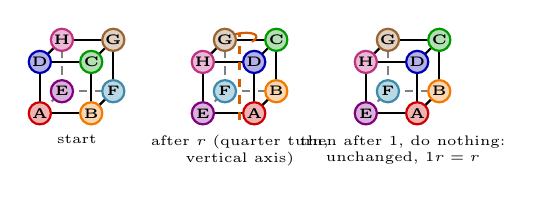
\begin{tikzpicture}[scale=0.45]
  \draw[thick] (0.000,0.000)--(1.450,0.000);
  \draw[thick] (1.450,0.000)--(1.450,1.450);
  \draw[thick] (1.450,1.450)--(0.000,1.450);
  \draw[thick] (0.000,1.450)--(0.000,0.000);
  \draw[thick] (1.450,0.000)--(2.073,0.623);
  \draw[thick] (2.073,0.623)--(2.073,2.073);
  \draw[thick] (2.073,2.073)--(1.450,1.450);
  \draw[thick] (0.000,1.450)--(0.623,2.073);
  \draw[thick] (0.623,2.073)--(2.073,2.073);
  \draw[thick,dashed,gray] (0.000,0.000)--(0.623,0.623);
  \draw[thick,dashed,gray] (0.623,0.623)--(2.073,0.623);
  \draw[thick,dashed,gray] (0.623,0.623)--(0.623,2.073);
  \node[font=\tiny\bfseries,circle,inner sep=0.3pt,minimum size=8pt,fill=red!80!black!30,draw=red!80!black,thick,text=black] at (0.000,0.000) {A};
  \node[font=\tiny\bfseries,circle,inner sep=0.3pt,minimum size=8pt,fill=orange!95!black!30,draw=orange!95!black,thick,text=black] at (1.450,0.000) {B};
  \node[font=\tiny\bfseries,circle,inner sep=0.3pt,minimum size=8pt,fill=green!60!black!30,draw=green!60!black,thick,text=black] at (1.450,1.450) {C};
  \node[font=\tiny\bfseries,circle,inner sep=0.3pt,minimum size=8pt,fill=blue!70!black!30,draw=blue!70!black,thick,text=black] at (0.000,1.450) {D};
  \node[font=\tiny\bfseries,circle,inner sep=0.3pt,minimum size=8pt,fill=violet!30,draw=violet,thick,text=black] at (0.623,0.623) {E};
  \node[font=\tiny\bfseries,circle,inner sep=0.3pt,minimum size=8pt,fill=cyan!65!black!30,draw=cyan!65!black,thick,text=black] at (2.073,0.623) {F};
  \node[font=\tiny\bfseries,circle,inner sep=0.3pt,minimum size=8pt,fill=brown!80!black!30,draw=brown!80!black,thick,text=black] at (2.073,2.073) {G};
  \node[font=\tiny\bfseries,circle,inner sep=0.3pt,minimum size=8pt,fill=magenta!75!black!30,draw=magenta!75!black,thick,text=black] at (0.623,2.073) {H};
  \node[font=\tiny,align=center,anchor=north] at (1.044,-0.350) {start};
  \draw[thick] (4.600,0.000)--(6.050,0.000);
  \draw[thick] (6.050,0.000)--(6.050,1.450);
  \draw[thick] (6.050,1.450)--(4.600,1.450);
  \draw[thick] (4.600,1.450)--(4.600,0.000);
  \draw[thick] (6.050,0.000)--(6.673,0.623);
  \draw[thick] (6.673,0.623)--(6.673,2.073);
  \draw[thick] (6.673,2.073)--(6.050,1.450);
  \draw[thick] (4.600,1.450)--(5.223,2.073);
  \draw[thick] (5.223,2.073)--(6.673,2.073);
  \draw[thick,dashed,gray] (4.600,0.000)--(5.223,0.623);
  \draw[thick,dashed,gray] (5.223,0.623)--(6.673,0.623);
  \draw[thick,dashed,gray] (5.223,0.623)--(5.223,2.073);
  \draw[dashed,thick,mkc] (5.637,-0.196)--(5.637,2.269);
  \draw[-{Stealth[length=2.5pt]},thick,mkc] (5.982,2.020)--(6.033,2.052)--(6.072,2.084)--(6.098,2.117)--(6.109,2.148)--(6.107,2.178)--(6.090,2.205)--(6.060,2.228)--(6.016,2.246)--(5.961,2.260)--(5.896,2.269)--(5.824,2.271)--(5.745,2.269)--(5.664,2.260)--(5.581,2.246)--(5.500,2.228)--(5.424,2.205)--(5.354,2.178)--(5.292,2.148)--(5.241,2.117)--(5.202,2.084)--(5.176,2.052)--(5.164,2.020)--(5.167,1.991)--(5.183,1.964);
  \node[font=\tiny\bfseries,circle,inner sep=0.3pt,minimum size=8pt,fill=red!80!black!30,draw=red!80!black,thick,text=black] at (6.050,0.000) {A};
  \node[font=\tiny\bfseries,circle,inner sep=0.3pt,minimum size=8pt,fill=orange!95!black!30,draw=orange!95!black,thick,text=black] at (6.673,0.623) {B};
  \node[font=\tiny\bfseries,circle,inner sep=0.3pt,minimum size=8pt,fill=green!60!black!30,draw=green!60!black,thick,text=black] at (6.673,2.073) {C};
  \node[font=\tiny\bfseries,circle,inner sep=0.3pt,minimum size=8pt,fill=blue!70!black!30,draw=blue!70!black,thick,text=black] at (6.050,1.450) {D};
  \node[font=\tiny\bfseries,circle,inner sep=0.3pt,minimum size=8pt,fill=violet!30,draw=violet,thick,text=black] at (4.600,0.000) {E};
  \node[font=\tiny\bfseries,circle,inner sep=0.3pt,minimum size=8pt,fill=cyan!65!black!30,draw=cyan!65!black,thick,text=black] at (5.223,0.623) {F};
  \node[font=\tiny\bfseries,circle,inner sep=0.3pt,minimum size=8pt,fill=brown!80!black!30,draw=brown!80!black,thick,text=black] at (5.223,2.073) {G};
  \node[font=\tiny\bfseries,circle,inner sep=0.3pt,minimum size=8pt,fill=magenta!75!black!30,draw=magenta!75!black,thick,text=black] at (4.600,1.450) {H};
  \node[font=\tiny,align=center,anchor=north] at (5.644,-0.350) {after $r$ (quarter turn,\\vertical axis)};
  \draw[thick] (9.200,0.000)--(10.650,0.000);
  \draw[thick] (10.650,0.000)--(10.650,1.450);
  \draw[thick] (10.650,1.450)--(9.200,1.450);
  \draw[thick] (9.200,1.450)--(9.200,0.000);
  \draw[thick] (10.650,0.000)--(11.273,0.623);
  \draw[thick] (11.273,0.623)--(11.273,2.073);
  \draw[thick] (11.273,2.073)--(10.650,1.450);
  \draw[thick] (9.200,1.450)--(9.823,2.073);
  \draw[thick] (9.823,2.073)--(11.273,2.073);
  \draw[thick,dashed,gray] (9.200,0.000)--(9.823,0.623);
  \draw[thick,dashed,gray] (9.823,0.623)--(11.273,0.623);
  \draw[thick,dashed,gray] (9.823,0.623)--(9.823,2.073);
  \node[font=\tiny\bfseries,circle,inner sep=0.3pt,minimum size=8pt,fill=red!80!black!30,draw=red!80!black,thick,text=black] at (10.650,0.000) {A};
  \node[font=\tiny\bfseries,circle,inner sep=0.3pt,minimum size=8pt,fill=orange!95!black!30,draw=orange!95!black,thick,text=black] at (11.273,0.623) {B};
  \node[font=\tiny\bfseries,circle,inner sep=0.3pt,minimum size=8pt,fill=green!60!black!30,draw=green!60!black,thick,text=black] at (11.273,2.073) {C};
  \node[font=\tiny\bfseries,circle,inner sep=0.3pt,minimum size=8pt,fill=blue!70!black!30,draw=blue!70!black,thick,text=black] at (10.650,1.450) {D};
  \node[font=\tiny\bfseries,circle,inner sep=0.3pt,minimum size=8pt,fill=violet!30,draw=violet,thick,text=black] at (9.200,0.000) {E};
  \node[font=\tiny\bfseries,circle,inner sep=0.3pt,minimum size=8pt,fill=cyan!65!black!30,draw=cyan!65!black,thick,text=black] at (9.823,0.623) {F};
  \node[font=\tiny\bfseries,circle,inner sep=0.3pt,minimum size=8pt,fill=brown!80!black!30,draw=brown!80!black,thick,text=black] at (9.823,2.073) {G};
  \node[font=\tiny\bfseries,circle,inner sep=0.3pt,minimum size=8pt,fill=magenta!75!black!30,draw=magenta!75!black,thick,text=black] at (9.200,1.450) {H};
  \node[font=\tiny,align=center,anchor=north] at (10.244,-0.350) {then after $1$, do nothing:\\unchanged, $1r=r$};
\end{tikzpicture}}\par\vspace{2pt}

\A{4}{Inverses: on the cube, ``turn it back''}
$g\inv$ is the move that cancels $g$; it is not ``$1/g$'' unless the group is numbers under multiplication. For the quarter turn $r$ the inverse is the quarter turn the other way, and three more turns forward do the same, so $r\inv=r^{3}$. Undo before or after, every disc returns home: $gh=hg=1$.\par\nobreak\vspace{2pt}
\centerline{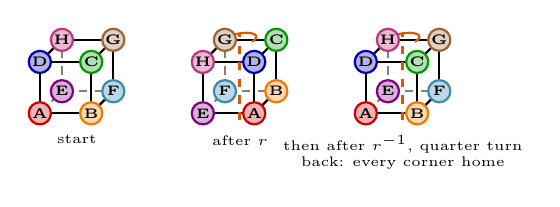
\begin{tikzpicture}[scale=0.45]
  \draw[thick] (0.000,0.000)--(1.450,0.000);
  \draw[thick] (1.450,0.000)--(1.450,1.450);
  \draw[thick] (1.450,1.450)--(0.000,1.450);
  \draw[thick] (0.000,1.450)--(0.000,0.000);
  \draw[thick] (1.450,0.000)--(2.073,0.623);
  \draw[thick] (2.073,0.623)--(2.073,2.073);
  \draw[thick] (2.073,2.073)--(1.450,1.450);
  \draw[thick] (0.000,1.450)--(0.623,2.073);
  \draw[thick] (0.623,2.073)--(2.073,2.073);
  \draw[thick,dashed,gray] (0.000,0.000)--(0.623,0.623);
  \draw[thick,dashed,gray] (0.623,0.623)--(2.073,0.623);
  \draw[thick,dashed,gray] (0.623,0.623)--(0.623,2.073);
  \node[font=\tiny\bfseries,circle,inner sep=0.3pt,minimum size=8pt,fill=red!80!black!30,draw=red!80!black,thick,text=black] at (0.000,0.000) {A};
  \node[font=\tiny\bfseries,circle,inner sep=0.3pt,minimum size=8pt,fill=orange!95!black!30,draw=orange!95!black,thick,text=black] at (1.450,0.000) {B};
  \node[font=\tiny\bfseries,circle,inner sep=0.3pt,minimum size=8pt,fill=green!60!black!30,draw=green!60!black,thick,text=black] at (1.450,1.450) {C};
  \node[font=\tiny\bfseries,circle,inner sep=0.3pt,minimum size=8pt,fill=blue!70!black!30,draw=blue!70!black,thick,text=black] at (0.000,1.450) {D};
  \node[font=\tiny\bfseries,circle,inner sep=0.3pt,minimum size=8pt,fill=violet!30,draw=violet,thick,text=black] at (0.623,0.623) {E};
  \node[font=\tiny\bfseries,circle,inner sep=0.3pt,minimum size=8pt,fill=cyan!65!black!30,draw=cyan!65!black,thick,text=black] at (2.073,0.623) {F};
  \node[font=\tiny\bfseries,circle,inner sep=0.3pt,minimum size=8pt,fill=brown!80!black!30,draw=brown!80!black,thick,text=black] at (2.073,2.073) {G};
  \node[font=\tiny\bfseries,circle,inner sep=0.3pt,minimum size=8pt,fill=magenta!75!black!30,draw=magenta!75!black,thick,text=black] at (0.623,2.073) {H};
  \node[font=\tiny,align=center,anchor=north] at (1.044,-0.350) {start};
  \draw[thick] (4.600,0.000)--(6.050,0.000);
  \draw[thick] (6.050,0.000)--(6.050,1.450);
  \draw[thick] (6.050,1.450)--(4.600,1.450);
  \draw[thick] (4.600,1.450)--(4.600,0.000);
  \draw[thick] (6.050,0.000)--(6.673,0.623);
  \draw[thick] (6.673,0.623)--(6.673,2.073);
  \draw[thick] (6.673,2.073)--(6.050,1.450);
  \draw[thick] (4.600,1.450)--(5.223,2.073);
  \draw[thick] (5.223,2.073)--(6.673,2.073);
  \draw[thick,dashed,gray] (4.600,0.000)--(5.223,0.623);
  \draw[thick,dashed,gray] (5.223,0.623)--(6.673,0.623);
  \draw[thick,dashed,gray] (5.223,0.623)--(5.223,2.073);
  \draw[dashed,thick,mkc] (5.637,-0.196)--(5.637,2.269);
  \draw[-{Stealth[length=2.5pt]},thick,mkc] (5.982,2.020)--(6.033,2.052)--(6.072,2.084)--(6.098,2.117)--(6.109,2.148)--(6.107,2.178)--(6.090,2.205)--(6.060,2.228)--(6.016,2.246)--(5.961,2.260)--(5.896,2.269)--(5.824,2.271)--(5.745,2.269)--(5.664,2.260)--(5.581,2.246)--(5.500,2.228)--(5.424,2.205)--(5.354,2.178)--(5.292,2.148)--(5.241,2.117)--(5.202,2.084)--(5.176,2.052)--(5.164,2.020)--(5.167,1.991)--(5.183,1.964);
  \node[font=\tiny\bfseries,circle,inner sep=0.3pt,minimum size=8pt,fill=red!80!black!30,draw=red!80!black,thick,text=black] at (6.050,0.000) {A};
  \node[font=\tiny\bfseries,circle,inner sep=0.3pt,minimum size=8pt,fill=orange!95!black!30,draw=orange!95!black,thick,text=black] at (6.673,0.623) {B};
  \node[font=\tiny\bfseries,circle,inner sep=0.3pt,minimum size=8pt,fill=green!60!black!30,draw=green!60!black,thick,text=black] at (6.673,2.073) {C};
  \node[font=\tiny\bfseries,circle,inner sep=0.3pt,minimum size=8pt,fill=blue!70!black!30,draw=blue!70!black,thick,text=black] at (6.050,1.450) {D};
  \node[font=\tiny\bfseries,circle,inner sep=0.3pt,minimum size=8pt,fill=violet!30,draw=violet,thick,text=black] at (4.600,0.000) {E};
  \node[font=\tiny\bfseries,circle,inner sep=0.3pt,minimum size=8pt,fill=cyan!65!black!30,draw=cyan!65!black,thick,text=black] at (5.223,0.623) {F};
  \node[font=\tiny\bfseries,circle,inner sep=0.3pt,minimum size=8pt,fill=brown!80!black!30,draw=brown!80!black,thick,text=black] at (5.223,2.073) {G};
  \node[font=\tiny\bfseries,circle,inner sep=0.3pt,minimum size=8pt,fill=magenta!75!black!30,draw=magenta!75!black,thick,text=black] at (4.600,1.450) {H};
  \node[font=\tiny,align=center,anchor=north] at (5.644,-0.350) {after $r$};
  \draw[thick] (9.200,0.000)--(10.650,0.000);
  \draw[thick] (10.650,0.000)--(10.650,1.450);
  \draw[thick] (10.650,1.450)--(9.200,1.450);
  \draw[thick] (9.200,1.450)--(9.200,0.000);
  \draw[thick] (10.650,0.000)--(11.273,0.623);
  \draw[thick] (11.273,0.623)--(11.273,2.073);
  \draw[thick] (11.273,2.073)--(10.650,1.450);
  \draw[thick] (9.200,1.450)--(9.823,2.073);
  \draw[thick] (9.823,2.073)--(11.273,2.073);
  \draw[thick,dashed,gray] (9.200,0.000)--(9.823,0.623);
  \draw[thick,dashed,gray] (9.823,0.623)--(11.273,0.623);
  \draw[thick,dashed,gray] (9.823,0.623)--(9.823,2.073);
  \draw[dashed,thick,mkc] (10.237,-0.196)--(10.237,2.269);
  \draw[-{Stealth[length=2.5pt]},thick,mkc] (10.582,2.020)--(10.633,2.052)--(10.672,2.084)--(10.698,2.117)--(10.709,2.148)--(10.707,2.178)--(10.690,2.205)--(10.660,2.228)--(10.616,2.246)--(10.561,2.260)--(10.496,2.269)--(10.424,2.271)--(10.345,2.269)--(10.264,2.260)--(10.181,2.246)--(10.100,2.228)--(10.024,2.205)--(9.954,2.178)--(9.892,2.148)--(9.841,2.117)--(9.802,2.084)--(9.776,2.052)--(9.764,2.020)--(9.767,1.991)--(9.783,1.964);
  \node[font=\tiny\bfseries,circle,inner sep=0.3pt,minimum size=8pt,fill=red!80!black!30,draw=red!80!black,thick,text=black] at (9.200,0.000) {A};
  \node[font=\tiny\bfseries,circle,inner sep=0.3pt,minimum size=8pt,fill=orange!95!black!30,draw=orange!95!black,thick,text=black] at (10.650,0.000) {B};
  \node[font=\tiny\bfseries,circle,inner sep=0.3pt,minimum size=8pt,fill=green!60!black!30,draw=green!60!black,thick,text=black] at (10.650,1.450) {C};
  \node[font=\tiny\bfseries,circle,inner sep=0.3pt,minimum size=8pt,fill=blue!70!black!30,draw=blue!70!black,thick,text=black] at (9.200,1.450) {D};
  \node[font=\tiny\bfseries,circle,inner sep=0.3pt,minimum size=8pt,fill=violet!30,draw=violet,thick,text=black] at (9.823,0.623) {E};
  \node[font=\tiny\bfseries,circle,inner sep=0.3pt,minimum size=8pt,fill=cyan!65!black!30,draw=cyan!65!black,thick,text=black] at (11.273,0.623) {F};
  \node[font=\tiny\bfseries,circle,inner sep=0.3pt,minimum size=8pt,fill=brown!80!black!30,draw=brown!80!black,thick,text=black] at (11.273,2.073) {G};
  \node[font=\tiny\bfseries,circle,inner sep=0.3pt,minimum size=8pt,fill=magenta!75!black!30,draw=magenta!75!black,thick,text=black] at (9.823,2.073) {H};
  \node[font=\tiny,align=center,anchor=north] at (10.244,-0.350) {then after $r^{-1}$, quarter turn\\back: every corner home};
\end{tikzpicture}}\par\vspace{2pt}

\A{5}{Associativity: brackets do not matter}
$fgh$ has one meaning. On the cube, $(fg)h$ and $f(gh)$ both put the corners through $h$, then $g$, then $f$; the brackets only say which two moves you merge into a single rotation first, so both land on the last cube below (Interlude K2 draws the merged versions). Composition of functions is always associative; the free group (page 12) is where this takes real work.\par\nobreak\vspace{2pt}
\centerline{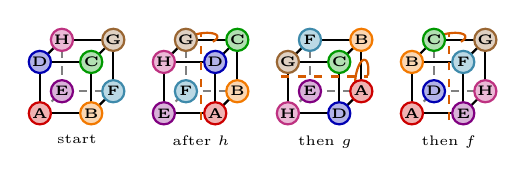
\begin{tikzpicture}[scale=0.45]
  \draw[thick] (0.000,0.000)--(1.450,0.000);
  \draw[thick] (1.450,0.000)--(1.450,1.450);
  \draw[thick] (1.450,1.450)--(0.000,1.450);
  \draw[thick] (0.000,1.450)--(0.000,0.000);
  \draw[thick] (1.450,0.000)--(2.073,0.623);
  \draw[thick] (2.073,0.623)--(2.073,2.073);
  \draw[thick] (2.073,2.073)--(1.450,1.450);
  \draw[thick] (0.000,1.450)--(0.623,2.073);
  \draw[thick] (0.623,2.073)--(2.073,2.073);
  \draw[thick,dashed,gray] (0.000,0.000)--(0.623,0.623);
  \draw[thick,dashed,gray] (0.623,0.623)--(2.073,0.623);
  \draw[thick,dashed,gray] (0.623,0.623)--(0.623,2.073);
  \node[font=\tiny\bfseries,circle,inner sep=0.3pt,minimum size=8pt,fill=red!80!black!30,draw=red!80!black,thick,text=black] at (0.000,0.000) {A};
  \node[font=\tiny\bfseries,circle,inner sep=0.3pt,minimum size=8pt,fill=orange!95!black!30,draw=orange!95!black,thick,text=black] at (1.450,0.000) {B};
  \node[font=\tiny\bfseries,circle,inner sep=0.3pt,minimum size=8pt,fill=green!60!black!30,draw=green!60!black,thick,text=black] at (1.450,1.450) {C};
  \node[font=\tiny\bfseries,circle,inner sep=0.3pt,minimum size=8pt,fill=blue!70!black!30,draw=blue!70!black,thick,text=black] at (0.000,1.450) {D};
  \node[font=\tiny\bfseries,circle,inner sep=0.3pt,minimum size=8pt,fill=violet!30,draw=violet,thick,text=black] at (0.623,0.623) {E};
  \node[font=\tiny\bfseries,circle,inner sep=0.3pt,minimum size=8pt,fill=cyan!65!black!30,draw=cyan!65!black,thick,text=black] at (2.073,0.623) {F};
  \node[font=\tiny\bfseries,circle,inner sep=0.3pt,minimum size=8pt,fill=brown!80!black!30,draw=brown!80!black,thick,text=black] at (2.073,2.073) {G};
  \node[font=\tiny\bfseries,circle,inner sep=0.3pt,minimum size=8pt,fill=magenta!75!black!30,draw=magenta!75!black,thick,text=black] at (0.623,2.073) {H};
  \node[font=\tiny,align=center,anchor=north] at (1.044,-0.350) {start};
  \draw[thick] (3.500,0.000)--(4.950,0.000);
  \draw[thick] (4.950,0.000)--(4.950,1.450);
  \draw[thick] (4.950,1.450)--(3.500,1.450);
  \draw[thick] (3.500,1.450)--(3.500,0.000);
  \draw[thick] (4.950,0.000)--(5.573,0.623);
  \draw[thick] (5.573,0.623)--(5.573,2.073);
  \draw[thick] (5.573,2.073)--(4.950,1.450);
  \draw[thick] (3.500,1.450)--(4.123,2.073);
  \draw[thick] (4.123,2.073)--(5.573,2.073);
  \draw[thick,dashed,gray] (3.500,0.000)--(4.123,0.623);
  \draw[thick,dashed,gray] (4.123,0.623)--(5.573,0.623);
  \draw[thick,dashed,gray] (4.123,0.623)--(4.123,2.073);
  \draw[dashed,thick,mkc] (4.537,-0.196)--(4.537,2.269);
  \draw[-{Stealth[length=2.5pt]},thick,mkc] (4.882,2.020)--(4.933,2.052)--(4.972,2.084)--(4.998,2.117)--(5.009,2.148)--(5.007,2.178)--(4.990,2.205)--(4.960,2.228)--(4.916,2.246)--(4.861,2.260)--(4.796,2.269)--(4.724,2.271)--(4.645,2.269)--(4.564,2.260)--(4.481,2.246)--(4.400,2.228)--(4.324,2.205)--(4.254,2.178)--(4.192,2.148)--(4.141,2.117)--(4.102,2.084)--(4.076,2.052)--(4.064,2.020)--(4.067,1.991)--(4.083,1.964);
  \node[font=\tiny\bfseries,circle,inner sep=0.3pt,minimum size=8pt,fill=red!80!black!30,draw=red!80!black,thick,text=black] at (4.950,0.000) {A};
  \node[font=\tiny\bfseries,circle,inner sep=0.3pt,minimum size=8pt,fill=orange!95!black!30,draw=orange!95!black,thick,text=black] at (5.573,0.623) {B};
  \node[font=\tiny\bfseries,circle,inner sep=0.3pt,minimum size=8pt,fill=green!60!black!30,draw=green!60!black,thick,text=black] at (5.573,2.073) {C};
  \node[font=\tiny\bfseries,circle,inner sep=0.3pt,minimum size=8pt,fill=blue!70!black!30,draw=blue!70!black,thick,text=black] at (4.950,1.450) {D};
  \node[font=\tiny\bfseries,circle,inner sep=0.3pt,minimum size=8pt,fill=violet!30,draw=violet,thick,text=black] at (3.500,0.000) {E};
  \node[font=\tiny\bfseries,circle,inner sep=0.3pt,minimum size=8pt,fill=cyan!65!black!30,draw=cyan!65!black,thick,text=black] at (4.123,0.623) {F};
  \node[font=\tiny\bfseries,circle,inner sep=0.3pt,minimum size=8pt,fill=brown!80!black!30,draw=brown!80!black,thick,text=black] at (4.123,2.073) {G};
  \node[font=\tiny\bfseries,circle,inner sep=0.3pt,minimum size=8pt,fill=magenta!75!black!30,draw=magenta!75!black,thick,text=black] at (3.500,1.450) {H};
  \node[font=\tiny,align=center,anchor=north] at (4.544,-0.350) {after $h$};
  \draw[thick] (7.000,0.000)--(8.450,0.000);
  \draw[thick] (8.450,0.000)--(8.450,1.450);
  \draw[thick] (8.450,1.450)--(7.000,1.450);
  \draw[thick] (7.000,1.450)--(7.000,0.000);
  \draw[thick] (8.450,0.000)--(9.073,0.623);
  \draw[thick] (9.073,0.623)--(9.073,2.073);
  \draw[thick] (9.073,2.073)--(8.450,1.450);
  \draw[thick] (7.000,1.450)--(7.623,2.073);
  \draw[thick] (7.623,2.073)--(9.073,2.073);
  \draw[thick,dashed,gray] (7.000,0.000)--(7.623,0.623);
  \draw[thick,dashed,gray] (7.623,0.623)--(9.073,0.623);
  \draw[thick,dashed,gray] (7.623,0.623)--(7.623,2.073);
  \draw[dashed,thick,mkc] (6.804,1.037)--(9.269,1.037);
  \draw[-{Stealth[length=2.5pt]},thick,mkc] (9.260,1.064)--(9.269,1.145)--(9.271,1.224)--(9.269,1.296)--(9.260,1.361)--(9.246,1.416)--(9.228,1.460)--(9.205,1.490)--(9.178,1.507)--(9.148,1.509)--(9.117,1.498)--(9.084,1.472)--(9.052,1.433)--(9.020,1.382)--(8.991,1.320)--(8.964,1.250)--(8.941,1.173)--(8.922,1.092)--(8.909,1.010)--(8.900,0.928)--(8.897,0.850)--(8.900,0.777)--(8.909,0.712)--(8.922,0.657)--(8.941,0.614);
  \node[font=\tiny\bfseries,circle,inner sep=0.3pt,minimum size=8pt,fill=red!80!black!30,draw=red!80!black,thick,text=black] at (9.073,0.623) {A};
  \node[font=\tiny\bfseries,circle,inner sep=0.3pt,minimum size=8pt,fill=orange!95!black!30,draw=orange!95!black,thick,text=black] at (9.073,2.073) {B};
  \node[font=\tiny\bfseries,circle,inner sep=0.3pt,minimum size=8pt,fill=green!60!black!30,draw=green!60!black,thick,text=black] at (8.450,1.450) {C};
  \node[font=\tiny\bfseries,circle,inner sep=0.3pt,minimum size=8pt,fill=blue!70!black!30,draw=blue!70!black,thick,text=black] at (8.450,0.000) {D};
  \node[font=\tiny\bfseries,circle,inner sep=0.3pt,minimum size=8pt,fill=violet!30,draw=violet,thick,text=black] at (7.623,0.623) {E};
  \node[font=\tiny\bfseries,circle,inner sep=0.3pt,minimum size=8pt,fill=cyan!65!black!30,draw=cyan!65!black,thick,text=black] at (7.623,2.073) {F};
  \node[font=\tiny\bfseries,circle,inner sep=0.3pt,minimum size=8pt,fill=brown!80!black!30,draw=brown!80!black,thick,text=black] at (7.000,1.450) {G};
  \node[font=\tiny\bfseries,circle,inner sep=0.3pt,minimum size=8pt,fill=magenta!75!black!30,draw=magenta!75!black,thick,text=black] at (7.000,0.000) {H};
  \node[font=\tiny,align=center,anchor=north] at (8.044,-0.350) {then $g$};
  \draw[thick] (10.500,0.000)--(11.950,0.000);
  \draw[thick] (11.950,0.000)--(11.950,1.450);
  \draw[thick] (11.950,1.450)--(10.500,1.450);
  \draw[thick] (10.500,1.450)--(10.500,0.000);
  \draw[thick] (11.950,0.000)--(12.573,0.623);
  \draw[thick] (12.573,0.623)--(12.573,2.073);
  \draw[thick] (12.573,2.073)--(11.950,1.450);
  \draw[thick] (10.500,1.450)--(11.123,2.073);
  \draw[thick] (11.123,2.073)--(12.573,2.073);
  \draw[thick,dashed,gray] (10.500,0.000)--(11.123,0.623);
  \draw[thick,dashed,gray] (11.123,0.623)--(12.573,0.623);
  \draw[thick,dashed,gray] (11.123,0.623)--(11.123,2.073);
  \draw[dashed,thick,mkc] (11.537,-0.196)--(11.537,2.269);
  \draw[-{Stealth[length=2.5pt]},thick,mkc] (11.882,2.020)--(11.933,2.052)--(11.972,2.084)--(11.998,2.117)--(12.009,2.148)--(12.007,2.178)--(11.990,2.205)--(11.960,2.228)--(11.916,2.246)--(11.861,2.260)--(11.796,2.269)--(11.724,2.271)--(11.645,2.269)--(11.564,2.260)--(11.481,2.246)--(11.400,2.228)--(11.324,2.205)--(11.254,2.178)--(11.192,2.148)--(11.141,2.117)--(11.102,2.084)--(11.076,2.052)--(11.064,2.020)--(11.067,1.991)--(11.083,1.964);
  \node[font=\tiny\bfseries,circle,inner sep=0.3pt,minimum size=8pt,fill=red!80!black!30,draw=red!80!black,thick,text=black] at (10.500,0.000) {A};
  \node[font=\tiny\bfseries,circle,inner sep=0.3pt,minimum size=8pt,fill=orange!95!black!30,draw=orange!95!black,thick,text=black] at (10.500,1.450) {B};
  \node[font=\tiny\bfseries,circle,inner sep=0.3pt,minimum size=8pt,fill=green!60!black!30,draw=green!60!black,thick,text=black] at (11.123,2.073) {C};
  \node[font=\tiny\bfseries,circle,inner sep=0.3pt,minimum size=8pt,fill=blue!70!black!30,draw=blue!70!black,thick,text=black] at (11.123,0.623) {D};
  \node[font=\tiny\bfseries,circle,inner sep=0.3pt,minimum size=8pt,fill=violet!30,draw=violet,thick,text=black] at (11.950,0.000) {E};
  \node[font=\tiny\bfseries,circle,inner sep=0.3pt,minimum size=8pt,fill=cyan!65!black!30,draw=cyan!65!black,thick,text=black] at (11.950,1.450) {F};
  \node[font=\tiny\bfseries,circle,inner sep=0.3pt,minimum size=8pt,fill=brown!80!black!30,draw=brown!80!black,thick,text=black] at (12.573,2.073) {G};
  \node[font=\tiny\bfseries,circle,inner sep=0.3pt,minimum size=8pt,fill=magenta!75!black!30,draw=magenta!75!black,thick,text=black] at (12.573,0.623) {H};
  \node[font=\tiny,align=center,anchor=north] at (11.544,-0.350) {then $f$};
\end{tikzpicture}}\par\vspace{2pt}

\begin{pitfall}
Nothing says $gh=hg$; groups where it holds are \emph{abelian} (page 17). The cube's group is not: $h$ then $g$ above differs from $g$ then $h$. Try it with a real cube.
\end{pitfall}

\A{6}{From the formal definition back to symmetries}
The next page checks the axioms for the cube in words. Interlude K takes the definition apart, with a checklist of examples and non-examples; Interlude K2 draws each axiom on the cube.
}

% ================================================================ INTERLUDE K (page 5: the definition of a group, unpacked)
\interlude{K. Page 5: the definition of a group, unpacked}{
\begin{minipage}[t]{744pt}\vspace{0pt}
\small
The definition on page 5 is short, but every word of it is load-bearing. This page takes it apart: what the data are, what the three promises say, which familiar objects pass the test and which fail, and why exactly these three promises are the right ones. The next Interlude then draws each promise on the cube.\par\vspace{6pt}
\begin{minipage}[t]{356pt}\vspace{0pt}
{\sffamily\bfseries\color{big} 1. Anatomy of the definition}\par\vspace{3pt}
\centering
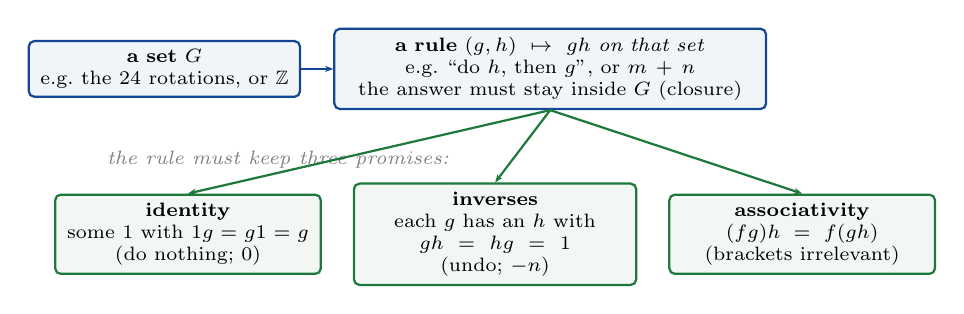
\begin{tikzpicture}[font=\scriptsize,>={Stealth[length=3pt]}]
  \node[draw=big,thick,rounded corners=2pt,fill=big!6,align=center,text width=92pt,inner sep=3pt] (set) at (0,0) {\textbf{a set $G$}\\ e.g.\ the 24 rotations, or $\Z$};
  \node[draw=big,thick,rounded corners=2pt,fill=big!6,align=center,text width=150pt,inner sep=3pt] (mul) at (4.9,0) {\textbf{a rule} $(g,h)\mapsto gh$ \emph{on that set}\\ e.g.\ ``do $h$, then $g$'', or $m+n$\\ the answer must stay inside $G$ (closure)};
  \node[font=\scriptsize\itshape,gray,anchor=west] at (-0.85,-1.15) {the rule must keep three promises:};
  \node[draw=why,thick,rounded corners=2pt,fill=why!6,align=center,text width=90pt,inner sep=3pt] (id) at (0.3,-2.1) {\textbf{identity}\\ some $1$ with $1g=g1=g$\\ (do nothing; $0$)};
  \node[draw=why,thick,rounded corners=2pt,fill=why!6,align=center,text width=96pt,inner sep=3pt] (inv) at (4.2,-2.1) {\textbf{inverses}\\ each $g$ has an $h$ with $gh=hg=1$\\ (undo; $-n$)};
  \node[draw=why,thick,rounded corners=2pt,fill=why!6,align=center,text width=90pt,inner sep=3pt] (as) at (8.1,-2.1) {\textbf{associativity}\\ $(fg)h=f(gh)$\\ (brackets irrelevant)};
  \draw[->,thick,big] (set)--(mul);
  \draw[->,thick,why] (mul.south) -- (id.north);
  \draw[->,thick,why] (mul.south) -- (inv.north);
  \draw[->,thick,why] (mul.south) -- (as.north);
\end{tikzpicture}\par\vspace{4pt}
\raggedright
The \emph{rule} is part of the data: the same set can be a group with one rule and fail with another ($\Z$ with $+$ passes, $\Z$ with $\times$ or $-$ fails; see the checklist). ``Multiplication'' is only a word for the rule; nothing about it need resemble multiplying numbers.\par\vspace{6pt}
{\sffamily\bfseries\color{big} 2. Why exactly these three promises?}\par\vspace{3pt}
They are precisely what is needed to \emph{solve equations}. Suppose $g$ and $k$ are known and you want the unknown $x$ with $gx=k$; on the cube: ``which move $x$, followed by $g$, gives $k$?''
\begin{center}
\begin{tabular}{@{}ll@{}}
$gx=k$ & given\\
$g^{-1}(gx)=g^{-1}k$ & apply $g^{-1}$ on the left of both sides \quad(\emph{inverses} exist)\\
$(g^{-1}g)x=g^{-1}k$ & regroup \quad(\emph{associativity})\\
$1\,x=g^{-1}k$ & $g^{-1}g=1$ \quad(\emph{inverses}, both sides needed)\\
$x=g^{-1}k$ & $1x=x$ \quad(\emph{identity})\\
\end{tabular}
\end{center}
Each promise is used exactly once, and the answer is unique: do $k$, then undo $g$. Drop any one axiom and this calculation breaks. That is also why the cancellation law $gx=gy\Rightarrow x=y$ holds in every group.
\end{minipage}\hfill
\begin{minipage}[t]{372pt}\vspace{0pt}
{\sffamily\bfseries\color{big} 3. Checklist: which of these are groups?}\par\vspace{3pt}
\centering
\begin{tabular}{@{}llccccl@{}}
\toprule
set & rule & closed & identity & inverses & assoc. & group?\\
\midrule
$\Z$ & $+$ & \cmark & $0$ & $-n$ & \cmark & yes\\
$\{0,1,2,\dots\}$ & $+$ & \cmark & $0$ & \xmark\ ($-5\notin$) & \cmark & no\\
$\Z$ & $-$ & \cmark & \xmark\ ($0-5\neq5$) & -- & \xmark & no\\
$\Z$ & $\times$ & \cmark & $1$ & \xmark\ ($\tfrac12\notin\Z$) & \cmark & no\\
$\{1,-1\}$ & $\times$ & \cmark & $1$ & each is its own & \cmark & yes\\
$\R$ & $\times$ & \cmark & $1$ & \xmark\ ($0$ has none) & \cmark & no\\
$\R\setminus\{0\}$ & $\times$ & \cmark & $1$ & $1/x$ & \cmark & yes\\
24 cube rotations & ``then'' & \cmark & do nothing & undo & \cmark & yes\\
the 6 quarter turns & ``then'' & \xmark & -- & -- & -- & no\\
$\{1,\ \text{3 face half turns}\}$ & ``then'' & \cmark & $1$ & each its own & \cmark & yes\\
\bottomrule
\end{tabular}\par\vspace{3pt}
\raggedright
For $\Z$ with $-$: $5-0=5$ but $0-5\neq5$, so $0$ is an identity on one side only, and $(8-4)-2\neq8-(4-2)$. Associativity never fails for symmetries, because ``do one, then the other'' is composition of functions.\par\vspace{6pt}
{\sffamily\bfseries\color{big} 4. Closure can fail inside the cube}\par\vspace{3pt}
The six quarter turns look like a natural family, but two of them in a row need not be a quarter turn, so the family is not closed under ``then'' and is not a group by itself:\par\vspace{2pt}
\centering
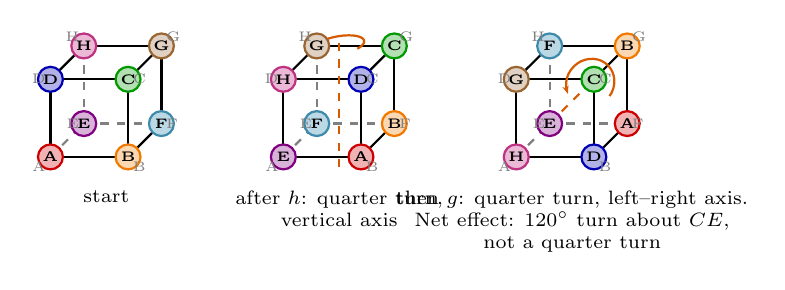
\begin{tikzpicture}[scale=0.68]
  \draw[thick] (0.000,0.000)--(1.450,0.000);
  \draw[thick] (1.450,0.000)--(1.450,1.450);
  \draw[thick] (1.450,1.450)--(0.000,1.450);
  \draw[thick] (0.000,1.450)--(0.000,0.000);
  \draw[thick] (1.450,0.000)--(2.073,0.623);
  \draw[thick] (2.073,0.623)--(2.073,2.073);
  \draw[thick] (2.073,2.073)--(1.450,1.450);
  \draw[thick] (0.000,1.450)--(0.623,2.073);
  \draw[thick] (0.623,2.073)--(2.073,2.073);
  \draw[thick,dashed,gray] (0.000,0.000)--(0.623,0.623);
  \draw[thick,dashed,gray] (0.623,0.623)--(2.073,0.623);
  \draw[thick,dashed,gray] (0.623,0.623)--(0.623,2.073);
  \node[font=\tiny\bfseries,circle,inner sep=0.5pt,minimum size=9pt,fill=red!80!black!30,draw=red!80!black,thick,text=black] at (0.000,0.000) {A};
  \node[font=\tiny,gray,below left,inner sep=1.5pt] at (0.000,0.000) {A};
  \node[font=\tiny\bfseries,circle,inner sep=0.5pt,minimum size=9pt,fill=orange!95!black!30,draw=orange!95!black,thick,text=black] at (1.450,0.000) {B};
  \node[font=\tiny,gray,below right,inner sep=1.5pt] at (1.450,0.000) {B};
  \node[font=\tiny\bfseries,circle,inner sep=0.5pt,minimum size=9pt,fill=green!60!black!30,draw=green!60!black,thick,text=black] at (1.450,1.450) {C};
  \node[font=\tiny,gray,right,inner sep=1.5pt] at (1.450,1.450) {C};
  \node[font=\tiny\bfseries,circle,inner sep=0.5pt,minimum size=9pt,fill=blue!70!black!30,draw=blue!70!black,thick,text=black] at (0.000,1.450) {D};
  \node[font=\tiny,gray,left,inner sep=1.5pt] at (0.000,1.450) {D};
  \node[font=\tiny\bfseries,circle,inner sep=0.5pt,minimum size=9pt,fill=violet!30,draw=violet,thick,text=black] at (0.623,0.623) {E};
  \node[font=\tiny,gray,left,inner sep=1.5pt] at (0.623,0.623) {E};
  \node[font=\tiny\bfseries,circle,inner sep=0.5pt,minimum size=9pt,fill=cyan!65!black!30,draw=cyan!65!black,thick,text=black] at (2.073,0.623) {F};
  \node[font=\tiny,gray,right,inner sep=1.5pt] at (2.073,0.623) {F};
  \node[font=\tiny\bfseries,circle,inner sep=0.5pt,minimum size=9pt,fill=brown!80!black!30,draw=brown!80!black,thick,text=black] at (2.073,2.073) {G};
  \node[font=\tiny,gray,above right,inner sep=1.5pt] at (2.073,2.073) {G};
  \node[font=\tiny\bfseries,circle,inner sep=0.5pt,minimum size=9pt,fill=magenta!75!black!30,draw=magenta!75!black,thick,text=black] at (0.623,2.073) {H};
  \node[font=\tiny,gray,above left,inner sep=1.5pt] at (0.623,2.073) {H};
  \node[font=\scriptsize,align=center,anchor=north] at (1.044,-0.450) {start};
  \draw[thick] (4.350,0.000)--(5.800,0.000);
  \draw[thick] (5.800,0.000)--(5.800,1.450);
  \draw[thick] (5.800,1.450)--(4.350,1.450);
  \draw[thick] (4.350,1.450)--(4.350,0.000);
  \draw[thick] (5.800,0.000)--(6.423,0.623);
  \draw[thick] (6.423,0.623)--(6.423,2.073);
  \draw[thick] (6.423,2.073)--(5.800,1.450);
  \draw[thick] (4.350,1.450)--(4.974,2.073);
  \draw[thick] (4.974,2.073)--(6.423,2.073);
  \draw[thick,dashed,gray] (4.350,0.000)--(4.974,0.623);
  \draw[thick,dashed,gray] (4.974,0.623)--(6.423,0.623);
  \draw[thick,dashed,gray] (4.974,0.623)--(4.974,2.073);
  \draw[dashed,thick,mkc] (5.387,-0.196)--(5.387,2.269);
  \draw[-{Stealth[length=3pt]},thick,mkc] (5.732,2.020)--(5.783,2.052)--(5.822,2.084)--(5.848,2.117)--(5.859,2.148)--(5.857,2.178)--(5.840,2.205)--(5.810,2.228)--(5.766,2.246)--(5.711,2.260)--(5.646,2.269)--(5.574,2.271)--(5.495,2.269)--(5.414,2.260)--(5.331,2.246)--(5.250,2.228)--(5.174,2.205)--(5.104,2.178)--(5.042,2.148)--(4.991,2.117)--(4.952,2.084)--(4.926,2.052)--(4.914,2.020)--(4.917,1.991)--(4.933,1.964);
  \node[font=\tiny\bfseries,circle,inner sep=0.5pt,minimum size=9pt,fill=red!80!black!30,draw=red!80!black,thick,text=black] at (5.800,0.000) {A};
  \node[font=\tiny,gray,below right,inner sep=1.5pt] at (5.800,0.000) {B};
  \node[font=\tiny\bfseries,circle,inner sep=0.5pt,minimum size=9pt,fill=orange!95!black!30,draw=orange!95!black,thick,text=black] at (6.423,0.623) {B};
  \node[font=\tiny,gray,right,inner sep=1.5pt] at (6.423,0.623) {F};
  \node[font=\tiny\bfseries,circle,inner sep=0.5pt,minimum size=9pt,fill=green!60!black!30,draw=green!60!black,thick,text=black] at (6.423,2.073) {C};
  \node[font=\tiny,gray,above right,inner sep=1.5pt] at (6.423,2.073) {G};
  \node[font=\tiny\bfseries,circle,inner sep=0.5pt,minimum size=9pt,fill=blue!70!black!30,draw=blue!70!black,thick,text=black] at (5.800,1.450) {D};
  \node[font=\tiny,gray,right,inner sep=1.5pt] at (5.800,1.450) {C};
  \node[font=\tiny\bfseries,circle,inner sep=0.5pt,minimum size=9pt,fill=violet!30,draw=violet,thick,text=black] at (4.350,0.000) {E};
  \node[font=\tiny,gray,below left,inner sep=1.5pt] at (4.350,0.000) {A};
  \node[font=\tiny\bfseries,circle,inner sep=0.5pt,minimum size=9pt,fill=cyan!65!black!30,draw=cyan!65!black,thick,text=black] at (4.974,0.623) {F};
  \node[font=\tiny,gray,left,inner sep=1.5pt] at (4.974,0.623) {E};
  \node[font=\tiny\bfseries,circle,inner sep=0.5pt,minimum size=9pt,fill=brown!80!black!30,draw=brown!80!black,thick,text=black] at (4.974,2.073) {G};
  \node[font=\tiny,gray,above left,inner sep=1.5pt] at (4.974,2.073) {H};
  \node[font=\tiny\bfseries,circle,inner sep=0.5pt,minimum size=9pt,fill=magenta!75!black!30,draw=magenta!75!black,thick,text=black] at (4.350,1.450) {H};
  \node[font=\tiny,gray,left,inner sep=1.5pt] at (4.350,1.450) {D};
  \node[font=\scriptsize,align=center,anchor=north] at (5.394,-0.450) {after $h$: quarter turn,\\vertical axis};
  \draw[thick] (8.700,0.000)--(10.150,0.000);
  \draw[thick] (10.150,0.000)--(10.150,1.450);
  \draw[thick] (10.150,1.450)--(8.700,1.450);
  \draw[thick] (8.700,1.450)--(8.700,0.000);
  \draw[thick] (10.150,0.000)--(10.773,0.623);
  \draw[thick] (10.773,0.623)--(10.773,2.073);
  \draw[thick] (10.773,2.073)--(10.150,1.450);
  \draw[thick] (8.700,1.450)--(9.324,2.073);
  \draw[thick] (9.324,2.073)--(10.773,2.073);
  \draw[thick,dashed,gray] (8.700,0.000)--(9.324,0.623);
  \draw[thick,dashed,gray] (9.324,0.623)--(10.773,0.623);
  \draw[thick,dashed,gray] (9.324,0.623)--(9.324,2.073);
  \draw[dashed,thick,mkc] (9.331,0.631)--(10.142,1.442);
  \draw[-{Stealth[length=3pt]},thick,mkc] (10.442,1.136)--(10.484,1.205)--(10.513,1.280)--(10.529,1.358)--(10.532,1.437)--(10.521,1.514)--(10.497,1.587)--(10.460,1.653)--(10.412,1.712)--(10.353,1.760)--(10.287,1.797)--(10.214,1.821)--(10.137,1.832)--(10.058,1.829)--(9.980,1.813)--(9.905,1.784)--(9.836,1.742)--(9.774,1.689)--(9.721,1.627)--(9.679,1.558)--(9.650,1.483)--(9.634,1.405)--(9.631,1.326)--(9.642,1.249)--(9.666,1.176);
  \node[font=\tiny\bfseries,circle,inner sep=0.5pt,minimum size=9pt,fill=red!80!black!30,draw=red!80!black,thick,text=black] at (10.773,0.623) {A};
  \node[font=\tiny,gray,right,inner sep=1.5pt] at (10.773,0.623) {F};
  \node[font=\tiny\bfseries,circle,inner sep=0.5pt,minimum size=9pt,fill=orange!95!black!30,draw=orange!95!black,thick,text=black] at (10.773,2.073) {B};
  \node[font=\tiny,gray,above right,inner sep=1.5pt] at (10.773,2.073) {G};
  \node[font=\tiny\bfseries,circle,inner sep=0.5pt,minimum size=9pt,fill=green!60!black!30,draw=green!60!black,thick,text=black] at (10.150,1.450) {C};
  \node[font=\tiny,gray,right,inner sep=1.5pt] at (10.150,1.450) {C};
  \node[font=\tiny\bfseries,circle,inner sep=0.5pt,minimum size=9pt,fill=blue!70!black!30,draw=blue!70!black,thick,text=black] at (10.150,0.000) {D};
  \node[font=\tiny,gray,below right,inner sep=1.5pt] at (10.150,0.000) {B};
  \node[font=\tiny\bfseries,circle,inner sep=0.5pt,minimum size=9pt,fill=violet!30,draw=violet,thick,text=black] at (9.324,0.623) {E};
  \node[font=\tiny,gray,left,inner sep=1.5pt] at (9.324,0.623) {E};
  \node[font=\tiny\bfseries,circle,inner sep=0.5pt,minimum size=9pt,fill=cyan!65!black!30,draw=cyan!65!black,thick,text=black] at (9.324,2.073) {F};
  \node[font=\tiny,gray,above left,inner sep=1.5pt] at (9.324,2.073) {H};
  \node[font=\tiny\bfseries,circle,inner sep=0.5pt,minimum size=9pt,fill=brown!80!black!30,draw=brown!80!black,thick,text=black] at (8.700,1.450) {G};
  \node[font=\tiny,gray,left,inner sep=1.5pt] at (8.700,1.450) {D};
  \node[font=\tiny\bfseries,circle,inner sep=0.5pt,minimum size=9pt,fill=magenta!75!black!30,draw=magenta!75!black,thick,text=black] at (8.700,0.000) {H};
  \node[font=\tiny,gray,below left,inner sep=1.5pt] at (8.700,0.000) {A};
  \node[font=\scriptsize,align=center,anchor=north] at (9.744,-0.450) {then $g$: quarter turn, left--right axis.\\Net effect: $120^\circ$ turn about $CE$,\\not a quarter turn};
\end{tikzpicture}

\raggedright
The last cube is the $120^\circ$ corner turn about the diagonal $CE$ (compare the dictionary in Interlude B2). The full set of 24 rotations \emph{is} closed: two rotations in a row are a rotation, because they are exactly the moves you can perform with the cube in your hands.
\end{minipage}
\par\vspace{6pt}
\begin{tryit}
Decide, using the checklist columns: the even integers with $+$; the odd integers with $+$; the 8 corner turns together with ``do nothing'' (hint: try two corner turns about different diagonals); the four rotations about a single face axis. Then solve $gx=k$ on the cube with $g$ a quarter turn about the vertical axis and $k$ the half turn about the same axis.
\end{tryit}
\end{minipage}
}

% ================================================================ INTERLUDE K2 (page 5: the three axioms on the cube)
\interlude{K2. Page 5: the three axioms, each checked on the cube}{
\begin{minipage}[t]{744pt}\vspace{0pt}
\small
The 24 rotations of the cube are the book's model group, so each axiom is tested on the cube itself, with the integers under addition as a one-line second example. Reading the pictures: grey letters are the fixed \emph{positions} $A,\dots,H$; the coloured disc at a position names the \emph{corner of the original cube} now sitting there, so a disc away from its grey letter has moved. An orange dashed line is the axis of the move just made; ``multiply'' means ``do the right-hand move, then the left-hand one'' (page 6).\par\vspace{6pt}
\begin{minipage}[t]{362pt}\vspace{0pt}
{\sffamily\bfseries\color{big} Identity: a move that changes nothing}\par\vspace{2pt}
``Leave the cube alone'' is a rotation (by $0^\circ$), and it is the identity: doing it after any move $r$ leaves the picture of $r$ untouched, and doing it before $r$ gives $r$ as well. So $1r=r1=r$.\par\vspace{2pt}
\centering
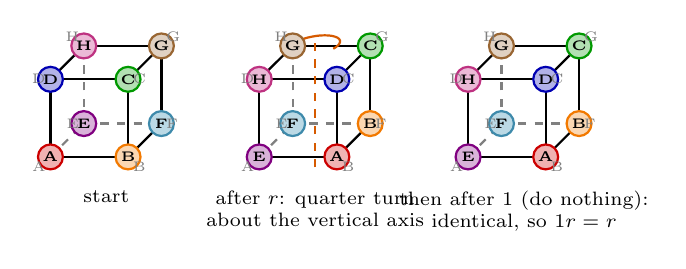
\begin{tikzpicture}[scale=0.68]
  \draw[thick] (0.000,0.000)--(1.450,0.000);
  \draw[thick] (1.450,0.000)--(1.450,1.450);
  \draw[thick] (1.450,1.450)--(0.000,1.450);
  \draw[thick] (0.000,1.450)--(0.000,0.000);
  \draw[thick] (1.450,0.000)--(2.073,0.623);
  \draw[thick] (2.073,0.623)--(2.073,2.073);
  \draw[thick] (2.073,2.073)--(1.450,1.450);
  \draw[thick] (0.000,1.450)--(0.623,2.073);
  \draw[thick] (0.623,2.073)--(2.073,2.073);
  \draw[thick,dashed,gray] (0.000,0.000)--(0.623,0.623);
  \draw[thick,dashed,gray] (0.623,0.623)--(2.073,0.623);
  \draw[thick,dashed,gray] (0.623,0.623)--(0.623,2.073);
  \node[font=\tiny\bfseries,circle,inner sep=0.5pt,minimum size=9pt,fill=red!80!black!30,draw=red!80!black,thick,text=black] at (0.000,0.000) {A};
  \node[font=\tiny,gray,below left,inner sep=1.5pt] at (0.000,0.000) {A};
  \node[font=\tiny\bfseries,circle,inner sep=0.5pt,minimum size=9pt,fill=orange!95!black!30,draw=orange!95!black,thick,text=black] at (1.450,0.000) {B};
  \node[font=\tiny,gray,below right,inner sep=1.5pt] at (1.450,0.000) {B};
  \node[font=\tiny\bfseries,circle,inner sep=0.5pt,minimum size=9pt,fill=green!60!black!30,draw=green!60!black,thick,text=black] at (1.450,1.450) {C};
  \node[font=\tiny,gray,right,inner sep=1.5pt] at (1.450,1.450) {C};
  \node[font=\tiny\bfseries,circle,inner sep=0.5pt,minimum size=9pt,fill=blue!70!black!30,draw=blue!70!black,thick,text=black] at (0.000,1.450) {D};
  \node[font=\tiny,gray,left,inner sep=1.5pt] at (0.000,1.450) {D};
  \node[font=\tiny\bfseries,circle,inner sep=0.5pt,minimum size=9pt,fill=violet!30,draw=violet,thick,text=black] at (0.623,0.623) {E};
  \node[font=\tiny,gray,left,inner sep=1.5pt] at (0.623,0.623) {E};
  \node[font=\tiny\bfseries,circle,inner sep=0.5pt,minimum size=9pt,fill=cyan!65!black!30,draw=cyan!65!black,thick,text=black] at (2.073,0.623) {F};
  \node[font=\tiny,gray,right,inner sep=1.5pt] at (2.073,0.623) {F};
  \node[font=\tiny\bfseries,circle,inner sep=0.5pt,minimum size=9pt,fill=brown!80!black!30,draw=brown!80!black,thick,text=black] at (2.073,2.073) {G};
  \node[font=\tiny,gray,above right,inner sep=1.5pt] at (2.073,2.073) {G};
  \node[font=\tiny\bfseries,circle,inner sep=0.5pt,minimum size=9pt,fill=magenta!75!black!30,draw=magenta!75!black,thick,text=black] at (0.623,2.073) {H};
  \node[font=\tiny,gray,above left,inner sep=1.5pt] at (0.623,2.073) {H};
  \node[font=\scriptsize,align=center,anchor=north] at (1.044,-0.450) {start};
  \draw[thick] (3.900,0.000)--(5.350,0.000);
  \draw[thick] (5.350,0.000)--(5.350,1.450);
  \draw[thick] (5.350,1.450)--(3.900,1.450);
  \draw[thick] (3.900,1.450)--(3.900,0.000);
  \draw[thick] (5.350,0.000)--(5.973,0.623);
  \draw[thick] (5.973,0.623)--(5.973,2.073);
  \draw[thick] (5.973,2.073)--(5.350,1.450);
  \draw[thick] (3.900,1.450)--(4.524,2.073);
  \draw[thick] (4.524,2.073)--(5.973,2.073);
  \draw[thick,dashed,gray] (3.900,0.000)--(4.524,0.623);
  \draw[thick,dashed,gray] (4.524,0.623)--(5.973,0.623);
  \draw[thick,dashed,gray] (4.524,0.623)--(4.524,2.073);
  \draw[dashed,thick,mkc] (4.937,-0.196)--(4.937,2.269);
  \draw[-{Stealth[length=3pt]},thick,mkc] (5.282,2.020)--(5.333,2.052)--(5.372,2.084)--(5.398,2.117)--(5.409,2.148)--(5.407,2.178)--(5.390,2.205)--(5.360,2.228)--(5.316,2.246)--(5.261,2.260)--(5.196,2.269)--(5.124,2.271)--(5.045,2.269)--(4.964,2.260)--(4.881,2.246)--(4.800,2.228)--(4.724,2.205)--(4.654,2.178)--(4.592,2.148)--(4.541,2.117)--(4.502,2.084)--(4.476,2.052)--(4.464,2.020)--(4.467,1.991)--(4.483,1.964);
  \node[font=\tiny\bfseries,circle,inner sep=0.5pt,minimum size=9pt,fill=red!80!black!30,draw=red!80!black,thick,text=black] at (5.350,0.000) {A};
  \node[font=\tiny,gray,below right,inner sep=1.5pt] at (5.350,0.000) {B};
  \node[font=\tiny\bfseries,circle,inner sep=0.5pt,minimum size=9pt,fill=orange!95!black!30,draw=orange!95!black,thick,text=black] at (5.973,0.623) {B};
  \node[font=\tiny,gray,right,inner sep=1.5pt] at (5.973,0.623) {F};
  \node[font=\tiny\bfseries,circle,inner sep=0.5pt,minimum size=9pt,fill=green!60!black!30,draw=green!60!black,thick,text=black] at (5.973,2.073) {C};
  \node[font=\tiny,gray,above right,inner sep=1.5pt] at (5.973,2.073) {G};
  \node[font=\tiny\bfseries,circle,inner sep=0.5pt,minimum size=9pt,fill=blue!70!black!30,draw=blue!70!black,thick,text=black] at (5.350,1.450) {D};
  \node[font=\tiny,gray,right,inner sep=1.5pt] at (5.350,1.450) {C};
  \node[font=\tiny\bfseries,circle,inner sep=0.5pt,minimum size=9pt,fill=violet!30,draw=violet,thick,text=black] at (3.900,0.000) {E};
  \node[font=\tiny,gray,below left,inner sep=1.5pt] at (3.900,0.000) {A};
  \node[font=\tiny\bfseries,circle,inner sep=0.5pt,minimum size=9pt,fill=cyan!65!black!30,draw=cyan!65!black,thick,text=black] at (4.524,0.623) {F};
  \node[font=\tiny,gray,left,inner sep=1.5pt] at (4.524,0.623) {E};
  \node[font=\tiny\bfseries,circle,inner sep=0.5pt,minimum size=9pt,fill=brown!80!black!30,draw=brown!80!black,thick,text=black] at (4.524,2.073) {G};
  \node[font=\tiny,gray,above left,inner sep=1.5pt] at (4.524,2.073) {H};
  \node[font=\tiny\bfseries,circle,inner sep=0.5pt,minimum size=9pt,fill=magenta!75!black!30,draw=magenta!75!black,thick,text=black] at (3.900,1.450) {H};
  \node[font=\tiny,gray,left,inner sep=1.5pt] at (3.900,1.450) {D};
  \node[font=\scriptsize,align=center,anchor=north] at (4.944,-0.450) {after $r$: quarter turn\\about the vertical axis};
  \draw[thick] (7.800,0.000)--(9.250,0.000);
  \draw[thick] (9.250,0.000)--(9.250,1.450);
  \draw[thick] (9.250,1.450)--(7.800,1.450);
  \draw[thick] (7.800,1.450)--(7.800,0.000);
  \draw[thick] (9.250,0.000)--(9.873,0.623);
  \draw[thick] (9.873,0.623)--(9.873,2.073);
  \draw[thick] (9.873,2.073)--(9.250,1.450);
  \draw[thick] (7.800,1.450)--(8.424,2.073);
  \draw[thick] (8.424,2.073)--(9.873,2.073);
  \draw[thick,dashed,gray] (7.800,0.000)--(8.424,0.623);
  \draw[thick,dashed,gray] (8.424,0.623)--(9.873,0.623);
  \draw[thick,dashed,gray] (8.424,0.623)--(8.424,2.073);
  \node[font=\tiny\bfseries,circle,inner sep=0.5pt,minimum size=9pt,fill=red!80!black!30,draw=red!80!black,thick,text=black] at (9.250,0.000) {A};
  \node[font=\tiny,gray,below right,inner sep=1.5pt] at (9.250,0.000) {B};
  \node[font=\tiny\bfseries,circle,inner sep=0.5pt,minimum size=9pt,fill=orange!95!black!30,draw=orange!95!black,thick,text=black] at (9.873,0.623) {B};
  \node[font=\tiny,gray,right,inner sep=1.5pt] at (9.873,0.623) {F};
  \node[font=\tiny\bfseries,circle,inner sep=0.5pt,minimum size=9pt,fill=green!60!black!30,draw=green!60!black,thick,text=black] at (9.873,2.073) {C};
  \node[font=\tiny,gray,above right,inner sep=1.5pt] at (9.873,2.073) {G};
  \node[font=\tiny\bfseries,circle,inner sep=0.5pt,minimum size=9pt,fill=blue!70!black!30,draw=blue!70!black,thick,text=black] at (9.250,1.450) {D};
  \node[font=\tiny,gray,right,inner sep=1.5pt] at (9.250,1.450) {C};
  \node[font=\tiny\bfseries,circle,inner sep=0.5pt,minimum size=9pt,fill=violet!30,draw=violet,thick,text=black] at (7.800,0.000) {E};
  \node[font=\tiny,gray,below left,inner sep=1.5pt] at (7.800,0.000) {A};
  \node[font=\tiny\bfseries,circle,inner sep=0.5pt,minimum size=9pt,fill=cyan!65!black!30,draw=cyan!65!black,thick,text=black] at (8.424,0.623) {F};
  \node[font=\tiny,gray,left,inner sep=1.5pt] at (8.424,0.623) {E};
  \node[font=\tiny\bfseries,circle,inner sep=0.5pt,minimum size=9pt,fill=brown!80!black!30,draw=brown!80!black,thick,text=black] at (8.424,2.073) {G};
  \node[font=\tiny,gray,above left,inner sep=1.5pt] at (8.424,2.073) {H};
  \node[font=\tiny\bfseries,circle,inner sep=0.5pt,minimum size=9pt,fill=magenta!75!black!30,draw=magenta!75!black,thick,text=black] at (7.800,1.450) {H};
  \node[font=\tiny,gray,left,inner sep=1.5pt] at (7.800,1.450) {D};
  \node[font=\scriptsize,align=center,anchor=north] at (8.844,-0.450) {then after $1$ (do nothing):\\identical, so $1r=r$};
\end{tikzpicture}

\raggedright
\emph{Integers:} the identity is $0$, not $1$: $0+5=5+0=5$, while $1+5\neq5$.\par\vspace{8pt}
{\sffamily\bfseries\color{big} Inverses: every move can be undone}\par\vspace{2pt}
The inverse of the quarter turn $r$ is the quarter turn the other way about the same axis; three more turns in the original direction do the same job, so $r^{-1}=r^{3}$. Undoing before or after both return every disc to its grey letter: $r^{-1}r=rr^{-1}=1$.\par\vspace{2pt}
\centering
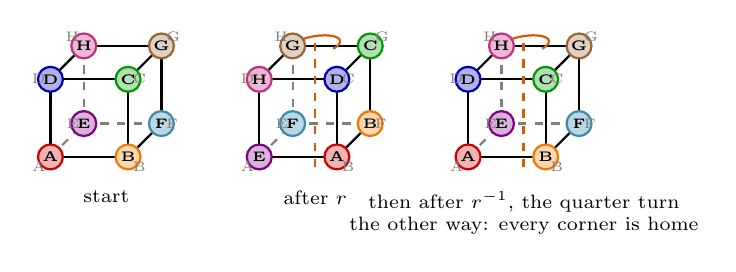
\begin{tikzpicture}[scale=0.68]
  \draw[thick] (0.000,0.000)--(1.450,0.000);
  \draw[thick] (1.450,0.000)--(1.450,1.450);
  \draw[thick] (1.450,1.450)--(0.000,1.450);
  \draw[thick] (0.000,1.450)--(0.000,0.000);
  \draw[thick] (1.450,0.000)--(2.073,0.623);
  \draw[thick] (2.073,0.623)--(2.073,2.073);
  \draw[thick] (2.073,2.073)--(1.450,1.450);
  \draw[thick] (0.000,1.450)--(0.623,2.073);
  \draw[thick] (0.623,2.073)--(2.073,2.073);
  \draw[thick,dashed,gray] (0.000,0.000)--(0.623,0.623);
  \draw[thick,dashed,gray] (0.623,0.623)--(2.073,0.623);
  \draw[thick,dashed,gray] (0.623,0.623)--(0.623,2.073);
  \node[font=\tiny\bfseries,circle,inner sep=0.5pt,minimum size=9pt,fill=red!80!black!30,draw=red!80!black,thick,text=black] at (0.000,0.000) {A};
  \node[font=\tiny,gray,below left,inner sep=1.5pt] at (0.000,0.000) {A};
  \node[font=\tiny\bfseries,circle,inner sep=0.5pt,minimum size=9pt,fill=orange!95!black!30,draw=orange!95!black,thick,text=black] at (1.450,0.000) {B};
  \node[font=\tiny,gray,below right,inner sep=1.5pt] at (1.450,0.000) {B};
  \node[font=\tiny\bfseries,circle,inner sep=0.5pt,minimum size=9pt,fill=green!60!black!30,draw=green!60!black,thick,text=black] at (1.450,1.450) {C};
  \node[font=\tiny,gray,right,inner sep=1.5pt] at (1.450,1.450) {C};
  \node[font=\tiny\bfseries,circle,inner sep=0.5pt,minimum size=9pt,fill=blue!70!black!30,draw=blue!70!black,thick,text=black] at (0.000,1.450) {D};
  \node[font=\tiny,gray,left,inner sep=1.5pt] at (0.000,1.450) {D};
  \node[font=\tiny\bfseries,circle,inner sep=0.5pt,minimum size=9pt,fill=violet!30,draw=violet,thick,text=black] at (0.623,0.623) {E};
  \node[font=\tiny,gray,left,inner sep=1.5pt] at (0.623,0.623) {E};
  \node[font=\tiny\bfseries,circle,inner sep=0.5pt,minimum size=9pt,fill=cyan!65!black!30,draw=cyan!65!black,thick,text=black] at (2.073,0.623) {F};
  \node[font=\tiny,gray,right,inner sep=1.5pt] at (2.073,0.623) {F};
  \node[font=\tiny\bfseries,circle,inner sep=0.5pt,minimum size=9pt,fill=brown!80!black!30,draw=brown!80!black,thick,text=black] at (2.073,2.073) {G};
  \node[font=\tiny,gray,above right,inner sep=1.5pt] at (2.073,2.073) {G};
  \node[font=\tiny\bfseries,circle,inner sep=0.5pt,minimum size=9pt,fill=magenta!75!black!30,draw=magenta!75!black,thick,text=black] at (0.623,2.073) {H};
  \node[font=\tiny,gray,above left,inner sep=1.5pt] at (0.623,2.073) {H};
  \node[font=\scriptsize,align=center,anchor=north] at (1.044,-0.450) {start};
  \draw[thick] (3.900,0.000)--(5.350,0.000);
  \draw[thick] (5.350,0.000)--(5.350,1.450);
  \draw[thick] (5.350,1.450)--(3.900,1.450);
  \draw[thick] (3.900,1.450)--(3.900,0.000);
  \draw[thick] (5.350,0.000)--(5.973,0.623);
  \draw[thick] (5.973,0.623)--(5.973,2.073);
  \draw[thick] (5.973,2.073)--(5.350,1.450);
  \draw[thick] (3.900,1.450)--(4.524,2.073);
  \draw[thick] (4.524,2.073)--(5.973,2.073);
  \draw[thick,dashed,gray] (3.900,0.000)--(4.524,0.623);
  \draw[thick,dashed,gray] (4.524,0.623)--(5.973,0.623);
  \draw[thick,dashed,gray] (4.524,0.623)--(4.524,2.073);
  \draw[dashed,thick,mkc] (4.937,-0.196)--(4.937,2.269);
  \draw[-{Stealth[length=3pt]},thick,mkc] (5.282,2.020)--(5.333,2.052)--(5.372,2.084)--(5.398,2.117)--(5.409,2.148)--(5.407,2.178)--(5.390,2.205)--(5.360,2.228)--(5.316,2.246)--(5.261,2.260)--(5.196,2.269)--(5.124,2.271)--(5.045,2.269)--(4.964,2.260)--(4.881,2.246)--(4.800,2.228)--(4.724,2.205)--(4.654,2.178)--(4.592,2.148)--(4.541,2.117)--(4.502,2.084)--(4.476,2.052)--(4.464,2.020)--(4.467,1.991)--(4.483,1.964);
  \node[font=\tiny\bfseries,circle,inner sep=0.5pt,minimum size=9pt,fill=red!80!black!30,draw=red!80!black,thick,text=black] at (5.350,0.000) {A};
  \node[font=\tiny,gray,below right,inner sep=1.5pt] at (5.350,0.000) {B};
  \node[font=\tiny\bfseries,circle,inner sep=0.5pt,minimum size=9pt,fill=orange!95!black!30,draw=orange!95!black,thick,text=black] at (5.973,0.623) {B};
  \node[font=\tiny,gray,right,inner sep=1.5pt] at (5.973,0.623) {F};
  \node[font=\tiny\bfseries,circle,inner sep=0.5pt,minimum size=9pt,fill=green!60!black!30,draw=green!60!black,thick,text=black] at (5.973,2.073) {C};
  \node[font=\tiny,gray,above right,inner sep=1.5pt] at (5.973,2.073) {G};
  \node[font=\tiny\bfseries,circle,inner sep=0.5pt,minimum size=9pt,fill=blue!70!black!30,draw=blue!70!black,thick,text=black] at (5.350,1.450) {D};
  \node[font=\tiny,gray,right,inner sep=1.5pt] at (5.350,1.450) {C};
  \node[font=\tiny\bfseries,circle,inner sep=0.5pt,minimum size=9pt,fill=violet!30,draw=violet,thick,text=black] at (3.900,0.000) {E};
  \node[font=\tiny,gray,below left,inner sep=1.5pt] at (3.900,0.000) {A};
  \node[font=\tiny\bfseries,circle,inner sep=0.5pt,minimum size=9pt,fill=cyan!65!black!30,draw=cyan!65!black,thick,text=black] at (4.524,0.623) {F};
  \node[font=\tiny,gray,left,inner sep=1.5pt] at (4.524,0.623) {E};
  \node[font=\tiny\bfseries,circle,inner sep=0.5pt,minimum size=9pt,fill=brown!80!black!30,draw=brown!80!black,thick,text=black] at (4.524,2.073) {G};
  \node[font=\tiny,gray,above left,inner sep=1.5pt] at (4.524,2.073) {H};
  \node[font=\tiny\bfseries,circle,inner sep=0.5pt,minimum size=9pt,fill=magenta!75!black!30,draw=magenta!75!black,thick,text=black] at (3.900,1.450) {H};
  \node[font=\tiny,gray,left,inner sep=1.5pt] at (3.900,1.450) {D};
  \node[font=\scriptsize,align=center,anchor=north] at (4.944,-0.450) {after $r$};
  \draw[thick] (7.800,0.000)--(9.250,0.000);
  \draw[thick] (9.250,0.000)--(9.250,1.450);
  \draw[thick] (9.250,1.450)--(7.800,1.450);
  \draw[thick] (7.800,1.450)--(7.800,0.000);
  \draw[thick] (9.250,0.000)--(9.873,0.623);
  \draw[thick] (9.873,0.623)--(9.873,2.073);
  \draw[thick] (9.873,2.073)--(9.250,1.450);
  \draw[thick] (7.800,1.450)--(8.424,2.073);
  \draw[thick] (8.424,2.073)--(9.873,2.073);
  \draw[thick,dashed,gray] (7.800,0.000)--(8.424,0.623);
  \draw[thick,dashed,gray] (8.424,0.623)--(9.873,0.623);
  \draw[thick,dashed,gray] (8.424,0.623)--(8.424,2.073);
  \draw[dashed,thick,mkc] (8.837,-0.196)--(8.837,2.269);
  \draw[-{Stealth[length=3pt]},thick,mkc] (9.182,2.020)--(9.233,2.052)--(9.272,2.084)--(9.298,2.117)--(9.309,2.148)--(9.307,2.178)--(9.290,2.205)--(9.260,2.228)--(9.216,2.246)--(9.161,2.260)--(9.096,2.269)--(9.024,2.271)--(8.945,2.269)--(8.864,2.260)--(8.781,2.246)--(8.700,2.228)--(8.624,2.205)--(8.554,2.178)--(8.492,2.148)--(8.441,2.117)--(8.402,2.084)--(8.376,2.052)--(8.364,2.020)--(8.367,1.991)--(8.383,1.964);
  \node[font=\tiny\bfseries,circle,inner sep=0.5pt,minimum size=9pt,fill=red!80!black!30,draw=red!80!black,thick,text=black] at (7.800,0.000) {A};
  \node[font=\tiny,gray,below left,inner sep=1.5pt] at (7.800,0.000) {A};
  \node[font=\tiny\bfseries,circle,inner sep=0.5pt,minimum size=9pt,fill=orange!95!black!30,draw=orange!95!black,thick,text=black] at (9.250,0.000) {B};
  \node[font=\tiny,gray,below right,inner sep=1.5pt] at (9.250,0.000) {B};
  \node[font=\tiny\bfseries,circle,inner sep=0.5pt,minimum size=9pt,fill=green!60!black!30,draw=green!60!black,thick,text=black] at (9.250,1.450) {C};
  \node[font=\tiny,gray,right,inner sep=1.5pt] at (9.250,1.450) {C};
  \node[font=\tiny\bfseries,circle,inner sep=0.5pt,minimum size=9pt,fill=blue!70!black!30,draw=blue!70!black,thick,text=black] at (7.800,1.450) {D};
  \node[font=\tiny,gray,left,inner sep=1.5pt] at (7.800,1.450) {D};
  \node[font=\tiny\bfseries,circle,inner sep=0.5pt,minimum size=9pt,fill=violet!30,draw=violet,thick,text=black] at (8.424,0.623) {E};
  \node[font=\tiny,gray,left,inner sep=1.5pt] at (8.424,0.623) {E};
  \node[font=\tiny\bfseries,circle,inner sep=0.5pt,minimum size=9pt,fill=cyan!65!black!30,draw=cyan!65!black,thick,text=black] at (9.873,0.623) {F};
  \node[font=\tiny,gray,right,inner sep=1.5pt] at (9.873,0.623) {F};
  \node[font=\tiny\bfseries,circle,inner sep=0.5pt,minimum size=9pt,fill=brown!80!black!30,draw=brown!80!black,thick,text=black] at (9.873,2.073) {G};
  \node[font=\tiny,gray,above right,inner sep=1.5pt] at (9.873,2.073) {G};
  \node[font=\tiny\bfseries,circle,inner sep=0.5pt,minimum size=9pt,fill=magenta!75!black!30,draw=magenta!75!black,thick,text=black] at (8.424,2.073) {H};
  \node[font=\tiny,gray,above left,inner sep=1.5pt] at (8.424,2.073) {H};
  \node[font=\scriptsize,align=center,anchor=north] at (8.844,-0.450) {then after $r^{-1}$, the quarter turn\\the other way: every corner is home};
\end{tikzpicture}

\raggedright
\emph{Integers:} the inverse of $5$ is $-5$, since $5+(-5)=(-5)+5=0$; it is not $1/5$, which cancels $5$ under the wrong operation. Half turns are their own inverses, like $0$ in $\Z$.
\end{minipage}\hfill
\begin{minipage}[t]{366pt}\vspace{0pt}
{\sffamily\bfseries\color{big} Associativity: brackets do not matter}\par\vspace{2pt}
Take three moves: $h$ a quarter turn about the vertical axis, $g$ a quarter turn about the left--right axis, $f$ a half turn about the vertical axis. Performed one after another they give this:\par\vspace{2pt}
\centering
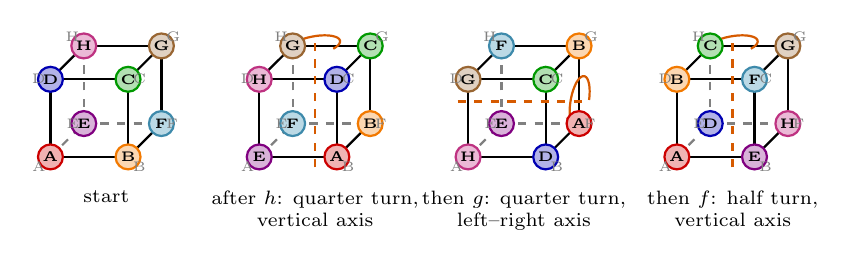
\begin{tikzpicture}[scale=0.68]
  \draw[thick] (0.000,0.000)--(1.450,0.000);
  \draw[thick] (1.450,0.000)--(1.450,1.450);
  \draw[thick] (1.450,1.450)--(0.000,1.450);
  \draw[thick] (0.000,1.450)--(0.000,0.000);
  \draw[thick] (1.450,0.000)--(2.073,0.623);
  \draw[thick] (2.073,0.623)--(2.073,2.073);
  \draw[thick] (2.073,2.073)--(1.450,1.450);
  \draw[thick] (0.000,1.450)--(0.623,2.073);
  \draw[thick] (0.623,2.073)--(2.073,2.073);
  \draw[thick,dashed,gray] (0.000,0.000)--(0.623,0.623);
  \draw[thick,dashed,gray] (0.623,0.623)--(2.073,0.623);
  \draw[thick,dashed,gray] (0.623,0.623)--(0.623,2.073);
  \node[font=\tiny\bfseries,circle,inner sep=0.5pt,minimum size=9pt,fill=red!80!black!30,draw=red!80!black,thick,text=black] at (0.000,0.000) {A};
  \node[font=\tiny,gray,below left,inner sep=1.5pt] at (0.000,0.000) {A};
  \node[font=\tiny\bfseries,circle,inner sep=0.5pt,minimum size=9pt,fill=orange!95!black!30,draw=orange!95!black,thick,text=black] at (1.450,0.000) {B};
  \node[font=\tiny,gray,below right,inner sep=1.5pt] at (1.450,0.000) {B};
  \node[font=\tiny\bfseries,circle,inner sep=0.5pt,minimum size=9pt,fill=green!60!black!30,draw=green!60!black,thick,text=black] at (1.450,1.450) {C};
  \node[font=\tiny,gray,right,inner sep=1.5pt] at (1.450,1.450) {C};
  \node[font=\tiny\bfseries,circle,inner sep=0.5pt,minimum size=9pt,fill=blue!70!black!30,draw=blue!70!black,thick,text=black] at (0.000,1.450) {D};
  \node[font=\tiny,gray,left,inner sep=1.5pt] at (0.000,1.450) {D};
  \node[font=\tiny\bfseries,circle,inner sep=0.5pt,minimum size=9pt,fill=violet!30,draw=violet,thick,text=black] at (0.623,0.623) {E};
  \node[font=\tiny,gray,left,inner sep=1.5pt] at (0.623,0.623) {E};
  \node[font=\tiny\bfseries,circle,inner sep=0.5pt,minimum size=9pt,fill=cyan!65!black!30,draw=cyan!65!black,thick,text=black] at (2.073,0.623) {F};
  \node[font=\tiny,gray,right,inner sep=1.5pt] at (2.073,0.623) {F};
  \node[font=\tiny\bfseries,circle,inner sep=0.5pt,minimum size=9pt,fill=brown!80!black!30,draw=brown!80!black,thick,text=black] at (2.073,2.073) {G};
  \node[font=\tiny,gray,above right,inner sep=1.5pt] at (2.073,2.073) {G};
  \node[font=\tiny\bfseries,circle,inner sep=0.5pt,minimum size=9pt,fill=magenta!75!black!30,draw=magenta!75!black,thick,text=black] at (0.623,2.073) {H};
  \node[font=\tiny,gray,above left,inner sep=1.5pt] at (0.623,2.073) {H};
  \node[font=\scriptsize,align=center,anchor=north] at (1.044,-0.450) {start};
  \draw[thick] (3.900,0.000)--(5.350,0.000);
  \draw[thick] (5.350,0.000)--(5.350,1.450);
  \draw[thick] (5.350,1.450)--(3.900,1.450);
  \draw[thick] (3.900,1.450)--(3.900,0.000);
  \draw[thick] (5.350,0.000)--(5.973,0.623);
  \draw[thick] (5.973,0.623)--(5.973,2.073);
  \draw[thick] (5.973,2.073)--(5.350,1.450);
  \draw[thick] (3.900,1.450)--(4.524,2.073);
  \draw[thick] (4.524,2.073)--(5.973,2.073);
  \draw[thick,dashed,gray] (3.900,0.000)--(4.524,0.623);
  \draw[thick,dashed,gray] (4.524,0.623)--(5.973,0.623);
  \draw[thick,dashed,gray] (4.524,0.623)--(4.524,2.073);
  \draw[dashed,thick,mkc] (4.937,-0.196)--(4.937,2.269);
  \draw[-{Stealth[length=3pt]},thick,mkc] (5.282,2.020)--(5.333,2.052)--(5.372,2.084)--(5.398,2.117)--(5.409,2.148)--(5.407,2.178)--(5.390,2.205)--(5.360,2.228)--(5.316,2.246)--(5.261,2.260)--(5.196,2.269)--(5.124,2.271)--(5.045,2.269)--(4.964,2.260)--(4.881,2.246)--(4.800,2.228)--(4.724,2.205)--(4.654,2.178)--(4.592,2.148)--(4.541,2.117)--(4.502,2.084)--(4.476,2.052)--(4.464,2.020)--(4.467,1.991)--(4.483,1.964);
  \node[font=\tiny\bfseries,circle,inner sep=0.5pt,minimum size=9pt,fill=red!80!black!30,draw=red!80!black,thick,text=black] at (5.350,0.000) {A};
  \node[font=\tiny,gray,below right,inner sep=1.5pt] at (5.350,0.000) {B};
  \node[font=\tiny\bfseries,circle,inner sep=0.5pt,minimum size=9pt,fill=orange!95!black!30,draw=orange!95!black,thick,text=black] at (5.973,0.623) {B};
  \node[font=\tiny,gray,right,inner sep=1.5pt] at (5.973,0.623) {F};
  \node[font=\tiny\bfseries,circle,inner sep=0.5pt,minimum size=9pt,fill=green!60!black!30,draw=green!60!black,thick,text=black] at (5.973,2.073) {C};
  \node[font=\tiny,gray,above right,inner sep=1.5pt] at (5.973,2.073) {G};
  \node[font=\tiny\bfseries,circle,inner sep=0.5pt,minimum size=9pt,fill=blue!70!black!30,draw=blue!70!black,thick,text=black] at (5.350,1.450) {D};
  \node[font=\tiny,gray,right,inner sep=1.5pt] at (5.350,1.450) {C};
  \node[font=\tiny\bfseries,circle,inner sep=0.5pt,minimum size=9pt,fill=violet!30,draw=violet,thick,text=black] at (3.900,0.000) {E};
  \node[font=\tiny,gray,below left,inner sep=1.5pt] at (3.900,0.000) {A};
  \node[font=\tiny\bfseries,circle,inner sep=0.5pt,minimum size=9pt,fill=cyan!65!black!30,draw=cyan!65!black,thick,text=black] at (4.524,0.623) {F};
  \node[font=\tiny,gray,left,inner sep=1.5pt] at (4.524,0.623) {E};
  \node[font=\tiny\bfseries,circle,inner sep=0.5pt,minimum size=9pt,fill=brown!80!black!30,draw=brown!80!black,thick,text=black] at (4.524,2.073) {G};
  \node[font=\tiny,gray,above left,inner sep=1.5pt] at (4.524,2.073) {H};
  \node[font=\tiny\bfseries,circle,inner sep=0.5pt,minimum size=9pt,fill=magenta!75!black!30,draw=magenta!75!black,thick,text=black] at (3.900,1.450) {H};
  \node[font=\tiny,gray,left,inner sep=1.5pt] at (3.900,1.450) {D};
  \node[font=\scriptsize,align=center,anchor=north] at (4.944,-0.450) {after $h$: quarter turn,\\vertical axis};
  \draw[thick] (7.800,0.000)--(9.250,0.000);
  \draw[thick] (9.250,0.000)--(9.250,1.450);
  \draw[thick] (9.250,1.450)--(7.800,1.450);
  \draw[thick] (7.800,1.450)--(7.800,0.000);
  \draw[thick] (9.250,0.000)--(9.873,0.623);
  \draw[thick] (9.873,0.623)--(9.873,2.073);
  \draw[thick] (9.873,2.073)--(9.250,1.450);
  \draw[thick] (7.800,1.450)--(8.424,2.073);
  \draw[thick] (8.424,2.073)--(9.873,2.073);
  \draw[thick,dashed,gray] (7.800,0.000)--(8.424,0.623);
  \draw[thick,dashed,gray] (8.424,0.623)--(9.873,0.623);
  \draw[thick,dashed,gray] (8.424,0.623)--(8.424,2.073);
  \draw[dashed,thick,mkc] (7.604,1.037)--(10.069,1.037);
  \draw[-{Stealth[length=3pt]},thick,mkc] (10.060,1.064)--(10.069,1.145)--(10.071,1.224)--(10.069,1.296)--(10.060,1.361)--(10.046,1.416)--(10.028,1.460)--(10.005,1.490)--(9.978,1.507)--(9.948,1.509)--(9.917,1.498)--(9.884,1.472)--(9.852,1.433)--(9.820,1.382)--(9.791,1.320)--(9.764,1.250)--(9.741,1.173)--(9.722,1.092)--(9.709,1.010)--(9.700,0.928)--(9.697,0.850)--(9.700,0.777)--(9.709,0.712)--(9.722,0.657)--(9.741,0.614);
  \node[font=\tiny\bfseries,circle,inner sep=0.5pt,minimum size=9pt,fill=red!80!black!30,draw=red!80!black,thick,text=black] at (9.873,0.623) {A};
  \node[font=\tiny,gray,right,inner sep=1.5pt] at (9.873,0.623) {F};
  \node[font=\tiny\bfseries,circle,inner sep=0.5pt,minimum size=9pt,fill=orange!95!black!30,draw=orange!95!black,thick,text=black] at (9.873,2.073) {B};
  \node[font=\tiny,gray,above right,inner sep=1.5pt] at (9.873,2.073) {G};
  \node[font=\tiny\bfseries,circle,inner sep=0.5pt,minimum size=9pt,fill=green!60!black!30,draw=green!60!black,thick,text=black] at (9.250,1.450) {C};
  \node[font=\tiny,gray,right,inner sep=1.5pt] at (9.250,1.450) {C};
  \node[font=\tiny\bfseries,circle,inner sep=0.5pt,minimum size=9pt,fill=blue!70!black!30,draw=blue!70!black,thick,text=black] at (9.250,0.000) {D};
  \node[font=\tiny,gray,below right,inner sep=1.5pt] at (9.250,0.000) {B};
  \node[font=\tiny\bfseries,circle,inner sep=0.5pt,minimum size=9pt,fill=violet!30,draw=violet,thick,text=black] at (8.424,0.623) {E};
  \node[font=\tiny,gray,left,inner sep=1.5pt] at (8.424,0.623) {E};
  \node[font=\tiny\bfseries,circle,inner sep=0.5pt,minimum size=9pt,fill=cyan!65!black!30,draw=cyan!65!black,thick,text=black] at (8.424,2.073) {F};
  \node[font=\tiny,gray,above left,inner sep=1.5pt] at (8.424,2.073) {H};
  \node[font=\tiny\bfseries,circle,inner sep=0.5pt,minimum size=9pt,fill=brown!80!black!30,draw=brown!80!black,thick,text=black] at (7.800,1.450) {G};
  \node[font=\tiny,gray,left,inner sep=1.5pt] at (7.800,1.450) {D};
  \node[font=\tiny\bfseries,circle,inner sep=0.5pt,minimum size=9pt,fill=magenta!75!black!30,draw=magenta!75!black,thick,text=black] at (7.800,0.000) {H};
  \node[font=\tiny,gray,below left,inner sep=1.5pt] at (7.800,0.000) {A};
  \node[font=\scriptsize,align=center,anchor=north] at (8.844,-0.450) {then $g$: quarter turn,\\left--right axis};
  \draw[thick] (11.700,0.000)--(13.150,0.000);
  \draw[thick] (13.150,0.000)--(13.150,1.450);
  \draw[thick] (13.150,1.450)--(11.700,1.450);
  \draw[thick] (11.700,1.450)--(11.700,0.000);
  \draw[thick] (13.150,0.000)--(13.773,0.623);
  \draw[thick] (13.773,0.623)--(13.773,2.073);
  \draw[thick] (13.773,2.073)--(13.150,1.450);
  \draw[thick] (11.700,1.450)--(12.323,2.073);
  \draw[thick] (12.323,2.073)--(13.773,2.073);
  \draw[thick,dashed,gray] (11.700,0.000)--(12.323,0.623);
  \draw[thick,dashed,gray] (12.323,0.623)--(13.773,0.623);
  \draw[thick,dashed,gray] (12.323,0.623)--(12.323,2.073);
  \draw[dashed,thick,mkc] (12.737,-0.196)--(12.737,2.269);
  \draw[-{Stealth[length=3pt]},thick,mkc] (13.082,2.020)--(13.133,2.052)--(13.172,2.084)--(13.198,2.117)--(13.209,2.148)--(13.207,2.178)--(13.190,2.205)--(13.160,2.228)--(13.116,2.246)--(13.061,2.260)--(12.996,2.269)--(12.924,2.271)--(12.845,2.269)--(12.764,2.260)--(12.681,2.246)--(12.600,2.228)--(12.524,2.205)--(12.454,2.178)--(12.392,2.148)--(12.341,2.117)--(12.302,2.084)--(12.276,2.052)--(12.264,2.020)--(12.267,1.991)--(12.283,1.964);
  \node[font=\tiny\bfseries,circle,inner sep=0.5pt,minimum size=9pt,fill=red!80!black!30,draw=red!80!black,thick,text=black] at (11.700,0.000) {A};
  \node[font=\tiny,gray,below left,inner sep=1.5pt] at (11.700,0.000) {A};
  \node[font=\tiny\bfseries,circle,inner sep=0.5pt,minimum size=9pt,fill=orange!95!black!30,draw=orange!95!black,thick,text=black] at (11.700,1.450) {B};
  \node[font=\tiny,gray,left,inner sep=1.5pt] at (11.700,1.450) {D};
  \node[font=\tiny\bfseries,circle,inner sep=0.5pt,minimum size=9pt,fill=green!60!black!30,draw=green!60!black,thick,text=black] at (12.323,2.073) {C};
  \node[font=\tiny,gray,above left,inner sep=1.5pt] at (12.323,2.073) {H};
  \node[font=\tiny\bfseries,circle,inner sep=0.5pt,minimum size=9pt,fill=blue!70!black!30,draw=blue!70!black,thick,text=black] at (12.323,0.623) {D};
  \node[font=\tiny,gray,left,inner sep=1.5pt] at (12.323,0.623) {E};
  \node[font=\tiny\bfseries,circle,inner sep=0.5pt,minimum size=9pt,fill=violet!30,draw=violet,thick,text=black] at (13.150,0.000) {E};
  \node[font=\tiny,gray,below right,inner sep=1.5pt] at (13.150,0.000) {B};
  \node[font=\tiny\bfseries,circle,inner sep=0.5pt,minimum size=9pt,fill=cyan!65!black!30,draw=cyan!65!black,thick,text=black] at (13.150,1.450) {F};
  \node[font=\tiny,gray,right,inner sep=1.5pt] at (13.150,1.450) {C};
  \node[font=\tiny\bfseries,circle,inner sep=0.5pt,minimum size=9pt,fill=brown!80!black!30,draw=brown!80!black,thick,text=black] at (13.773,2.073) {G};
  \node[font=\tiny,gray,above right,inner sep=1.5pt] at (13.773,2.073) {G};
  \node[font=\tiny\bfseries,circle,inner sep=0.5pt,minimum size=9pt,fill=magenta!75!black!30,draw=magenta!75!black,thick,text=black] at (13.773,0.623) {H};
  \node[font=\tiny,gray,right,inner sep=1.5pt] at (13.773,0.623) {F};
  \node[font=\scriptsize,align=center,anchor=north] at (12.744,-0.450) {then $f$: half turn,\\vertical axis};
\end{tikzpicture}

\raggedright
$(fg)h$ means: do $h$, then the \emph{single} rotation that $fg$ amounts to. $f(gh)$ means: do the single rotation $gh$, then $f$. Both end at the same cube as the row above:\par\vspace{2pt}
\centering
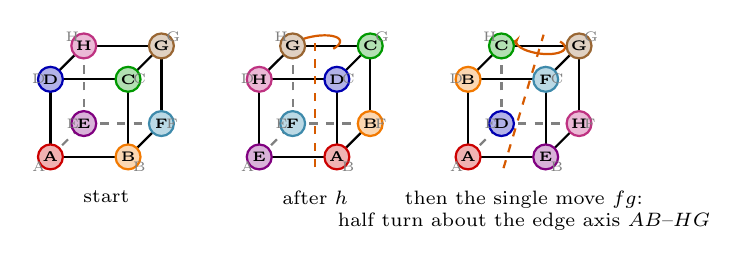
\begin{tikzpicture}[scale=0.68]
  \draw[thick] (0.000,0.000)--(1.450,0.000);
  \draw[thick] (1.450,0.000)--(1.450,1.450);
  \draw[thick] (1.450,1.450)--(0.000,1.450);
  \draw[thick] (0.000,1.450)--(0.000,0.000);
  \draw[thick] (1.450,0.000)--(2.073,0.623);
  \draw[thick] (2.073,0.623)--(2.073,2.073);
  \draw[thick] (2.073,2.073)--(1.450,1.450);
  \draw[thick] (0.000,1.450)--(0.623,2.073);
  \draw[thick] (0.623,2.073)--(2.073,2.073);
  \draw[thick,dashed,gray] (0.000,0.000)--(0.623,0.623);
  \draw[thick,dashed,gray] (0.623,0.623)--(2.073,0.623);
  \draw[thick,dashed,gray] (0.623,0.623)--(0.623,2.073);
  \node[font=\tiny\bfseries,circle,inner sep=0.5pt,minimum size=9pt,fill=red!80!black!30,draw=red!80!black,thick,text=black] at (0.000,0.000) {A};
  \node[font=\tiny,gray,below left,inner sep=1.5pt] at (0.000,0.000) {A};
  \node[font=\tiny\bfseries,circle,inner sep=0.5pt,minimum size=9pt,fill=orange!95!black!30,draw=orange!95!black,thick,text=black] at (1.450,0.000) {B};
  \node[font=\tiny,gray,below right,inner sep=1.5pt] at (1.450,0.000) {B};
  \node[font=\tiny\bfseries,circle,inner sep=0.5pt,minimum size=9pt,fill=green!60!black!30,draw=green!60!black,thick,text=black] at (1.450,1.450) {C};
  \node[font=\tiny,gray,right,inner sep=1.5pt] at (1.450,1.450) {C};
  \node[font=\tiny\bfseries,circle,inner sep=0.5pt,minimum size=9pt,fill=blue!70!black!30,draw=blue!70!black,thick,text=black] at (0.000,1.450) {D};
  \node[font=\tiny,gray,left,inner sep=1.5pt] at (0.000,1.450) {D};
  \node[font=\tiny\bfseries,circle,inner sep=0.5pt,minimum size=9pt,fill=violet!30,draw=violet,thick,text=black] at (0.623,0.623) {E};
  \node[font=\tiny,gray,left,inner sep=1.5pt] at (0.623,0.623) {E};
  \node[font=\tiny\bfseries,circle,inner sep=0.5pt,minimum size=9pt,fill=cyan!65!black!30,draw=cyan!65!black,thick,text=black] at (2.073,0.623) {F};
  \node[font=\tiny,gray,right,inner sep=1.5pt] at (2.073,0.623) {F};
  \node[font=\tiny\bfseries,circle,inner sep=0.5pt,minimum size=9pt,fill=brown!80!black!30,draw=brown!80!black,thick,text=black] at (2.073,2.073) {G};
  \node[font=\tiny,gray,above right,inner sep=1.5pt] at (2.073,2.073) {G};
  \node[font=\tiny\bfseries,circle,inner sep=0.5pt,minimum size=9pt,fill=magenta!75!black!30,draw=magenta!75!black,thick,text=black] at (0.623,2.073) {H};
  \node[font=\tiny,gray,above left,inner sep=1.5pt] at (0.623,2.073) {H};
  \node[font=\scriptsize,align=center,anchor=north] at (1.044,-0.450) {start};
  \draw[thick] (3.900,0.000)--(5.350,0.000);
  \draw[thick] (5.350,0.000)--(5.350,1.450);
  \draw[thick] (5.350,1.450)--(3.900,1.450);
  \draw[thick] (3.900,1.450)--(3.900,0.000);
  \draw[thick] (5.350,0.000)--(5.973,0.623);
  \draw[thick] (5.973,0.623)--(5.973,2.073);
  \draw[thick] (5.973,2.073)--(5.350,1.450);
  \draw[thick] (3.900,1.450)--(4.524,2.073);
  \draw[thick] (4.524,2.073)--(5.973,2.073);
  \draw[thick,dashed,gray] (3.900,0.000)--(4.524,0.623);
  \draw[thick,dashed,gray] (4.524,0.623)--(5.973,0.623);
  \draw[thick,dashed,gray] (4.524,0.623)--(4.524,2.073);
  \draw[dashed,thick,mkc] (4.937,-0.196)--(4.937,2.269);
  \draw[-{Stealth[length=3pt]},thick,mkc] (5.282,2.020)--(5.333,2.052)--(5.372,2.084)--(5.398,2.117)--(5.409,2.148)--(5.407,2.178)--(5.390,2.205)--(5.360,2.228)--(5.316,2.246)--(5.261,2.260)--(5.196,2.269)--(5.124,2.271)--(5.045,2.269)--(4.964,2.260)--(4.881,2.246)--(4.800,2.228)--(4.724,2.205)--(4.654,2.178)--(4.592,2.148)--(4.541,2.117)--(4.502,2.084)--(4.476,2.052)--(4.464,2.020)--(4.467,1.991)--(4.483,1.964);
  \node[font=\tiny\bfseries,circle,inner sep=0.5pt,minimum size=9pt,fill=red!80!black!30,draw=red!80!black,thick,text=black] at (5.350,0.000) {A};
  \node[font=\tiny,gray,below right,inner sep=1.5pt] at (5.350,0.000) {B};
  \node[font=\tiny\bfseries,circle,inner sep=0.5pt,minimum size=9pt,fill=orange!95!black!30,draw=orange!95!black,thick,text=black] at (5.973,0.623) {B};
  \node[font=\tiny,gray,right,inner sep=1.5pt] at (5.973,0.623) {F};
  \node[font=\tiny\bfseries,circle,inner sep=0.5pt,minimum size=9pt,fill=green!60!black!30,draw=green!60!black,thick,text=black] at (5.973,2.073) {C};
  \node[font=\tiny,gray,above right,inner sep=1.5pt] at (5.973,2.073) {G};
  \node[font=\tiny\bfseries,circle,inner sep=0.5pt,minimum size=9pt,fill=blue!70!black!30,draw=blue!70!black,thick,text=black] at (5.350,1.450) {D};
  \node[font=\tiny,gray,right,inner sep=1.5pt] at (5.350,1.450) {C};
  \node[font=\tiny\bfseries,circle,inner sep=0.5pt,minimum size=9pt,fill=violet!30,draw=violet,thick,text=black] at (3.900,0.000) {E};
  \node[font=\tiny,gray,below left,inner sep=1.5pt] at (3.900,0.000) {A};
  \node[font=\tiny\bfseries,circle,inner sep=0.5pt,minimum size=9pt,fill=cyan!65!black!30,draw=cyan!65!black,thick,text=black] at (4.524,0.623) {F};
  \node[font=\tiny,gray,left,inner sep=1.5pt] at (4.524,0.623) {E};
  \node[font=\tiny\bfseries,circle,inner sep=0.5pt,minimum size=9pt,fill=brown!80!black!30,draw=brown!80!black,thick,text=black] at (4.524,2.073) {G};
  \node[font=\tiny,gray,above left,inner sep=1.5pt] at (4.524,2.073) {H};
  \node[font=\tiny\bfseries,circle,inner sep=0.5pt,minimum size=9pt,fill=magenta!75!black!30,draw=magenta!75!black,thick,text=black] at (3.900,1.450) {H};
  \node[font=\tiny,gray,left,inner sep=1.5pt] at (3.900,1.450) {D};
  \node[font=\scriptsize,align=center,anchor=north] at (4.944,-0.450) {after $h$};
  \draw[thick] (7.800,0.000)--(9.250,0.000);
  \draw[thick] (9.250,0.000)--(9.250,1.450);
  \draw[thick] (9.250,1.450)--(7.800,1.450);
  \draw[thick] (7.800,1.450)--(7.800,0.000);
  \draw[thick] (9.250,0.000)--(9.873,0.623);
  \draw[thick] (9.873,0.623)--(9.873,2.073);
  \draw[thick] (9.873,2.073)--(9.250,1.450);
  \draw[thick] (7.800,1.450)--(8.424,2.073);
  \draw[thick] (8.424,2.073)--(9.873,2.073);
  \draw[thick,dashed,gray] (7.800,0.000)--(8.424,0.623);
  \draw[thick,dashed,gray] (8.424,0.623)--(9.873,0.623);
  \draw[thick,dashed,gray] (8.424,0.623)--(8.424,2.073);
  \draw[dashed,thick,mkc] (8.462,-0.210)--(9.211,2.283);
  \draw[-{Stealth[length=3pt]},thick,mkc] (9.519,2.156)--(9.561,2.127)--(9.590,2.096)--(9.607,2.066)--(9.609,2.036)--(9.598,2.008)--(9.574,1.983)--(9.536,1.962)--(9.487,1.944)--(9.428,1.931)--(9.361,1.923)--(9.288,1.921)--(9.210,1.923)--(9.131,1.931)--(9.052,1.944)--(8.977,1.962)--(8.907,1.983)--(8.845,2.008)--(8.792,2.036)--(8.750,2.066)--(8.720,2.096)--(8.704,2.127)--(8.701,2.156)--(8.712,2.184)--(8.737,2.209);
  \node[font=\tiny\bfseries,circle,inner sep=0.5pt,minimum size=9pt,fill=red!80!black!30,draw=red!80!black,thick,text=black] at (7.800,0.000) {A};
  \node[font=\tiny,gray,below left,inner sep=1.5pt] at (7.800,0.000) {A};
  \node[font=\tiny\bfseries,circle,inner sep=0.5pt,minimum size=9pt,fill=orange!95!black!30,draw=orange!95!black,thick,text=black] at (7.800,1.450) {B};
  \node[font=\tiny,gray,left,inner sep=1.5pt] at (7.800,1.450) {D};
  \node[font=\tiny\bfseries,circle,inner sep=0.5pt,minimum size=9pt,fill=green!60!black!30,draw=green!60!black,thick,text=black] at (8.424,2.073) {C};
  \node[font=\tiny,gray,above left,inner sep=1.5pt] at (8.424,2.073) {H};
  \node[font=\tiny\bfseries,circle,inner sep=0.5pt,minimum size=9pt,fill=blue!70!black!30,draw=blue!70!black,thick,text=black] at (8.424,0.623) {D};
  \node[font=\tiny,gray,left,inner sep=1.5pt] at (8.424,0.623) {E};
  \node[font=\tiny\bfseries,circle,inner sep=0.5pt,minimum size=9pt,fill=violet!30,draw=violet,thick,text=black] at (9.250,0.000) {E};
  \node[font=\tiny,gray,below right,inner sep=1.5pt] at (9.250,0.000) {B};
  \node[font=\tiny\bfseries,circle,inner sep=0.5pt,minimum size=9pt,fill=cyan!65!black!30,draw=cyan!65!black,thick,text=black] at (9.250,1.450) {F};
  \node[font=\tiny,gray,right,inner sep=1.5pt] at (9.250,1.450) {C};
  \node[font=\tiny\bfseries,circle,inner sep=0.5pt,minimum size=9pt,fill=brown!80!black!30,draw=brown!80!black,thick,text=black] at (9.873,2.073) {G};
  \node[font=\tiny,gray,above right,inner sep=1.5pt] at (9.873,2.073) {G};
  \node[font=\tiny\bfseries,circle,inner sep=0.5pt,minimum size=9pt,fill=magenta!75!black!30,draw=magenta!75!black,thick,text=black] at (9.873,0.623) {H};
  \node[font=\tiny,gray,right,inner sep=1.5pt] at (9.873,0.623) {F};
  \node[font=\scriptsize,align=center,anchor=north] at (8.844,-0.450) {then the single move $fg$:\\half turn about the edge axis $AB$--$HG$};
\end{tikzpicture}

\par\vspace{2pt}
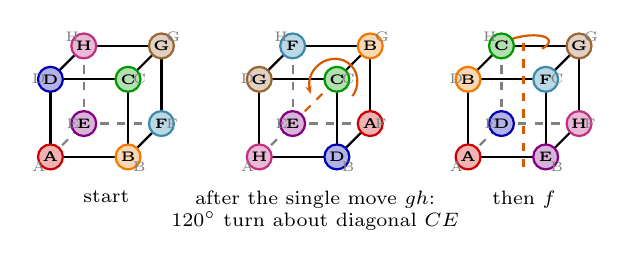
\begin{tikzpicture}[scale=0.68]
  \draw[thick] (0.000,0.000)--(1.450,0.000);
  \draw[thick] (1.450,0.000)--(1.450,1.450);
  \draw[thick] (1.450,1.450)--(0.000,1.450);
  \draw[thick] (0.000,1.450)--(0.000,0.000);
  \draw[thick] (1.450,0.000)--(2.073,0.623);
  \draw[thick] (2.073,0.623)--(2.073,2.073);
  \draw[thick] (2.073,2.073)--(1.450,1.450);
  \draw[thick] (0.000,1.450)--(0.623,2.073);
  \draw[thick] (0.623,2.073)--(2.073,2.073);
  \draw[thick,dashed,gray] (0.000,0.000)--(0.623,0.623);
  \draw[thick,dashed,gray] (0.623,0.623)--(2.073,0.623);
  \draw[thick,dashed,gray] (0.623,0.623)--(0.623,2.073);
  \node[font=\tiny\bfseries,circle,inner sep=0.5pt,minimum size=9pt,fill=red!80!black!30,draw=red!80!black,thick,text=black] at (0.000,0.000) {A};
  \node[font=\tiny,gray,below left,inner sep=1.5pt] at (0.000,0.000) {A};
  \node[font=\tiny\bfseries,circle,inner sep=0.5pt,minimum size=9pt,fill=orange!95!black!30,draw=orange!95!black,thick,text=black] at (1.450,0.000) {B};
  \node[font=\tiny,gray,below right,inner sep=1.5pt] at (1.450,0.000) {B};
  \node[font=\tiny\bfseries,circle,inner sep=0.5pt,minimum size=9pt,fill=green!60!black!30,draw=green!60!black,thick,text=black] at (1.450,1.450) {C};
  \node[font=\tiny,gray,right,inner sep=1.5pt] at (1.450,1.450) {C};
  \node[font=\tiny\bfseries,circle,inner sep=0.5pt,minimum size=9pt,fill=blue!70!black!30,draw=blue!70!black,thick,text=black] at (0.000,1.450) {D};
  \node[font=\tiny,gray,left,inner sep=1.5pt] at (0.000,1.450) {D};
  \node[font=\tiny\bfseries,circle,inner sep=0.5pt,minimum size=9pt,fill=violet!30,draw=violet,thick,text=black] at (0.623,0.623) {E};
  \node[font=\tiny,gray,left,inner sep=1.5pt] at (0.623,0.623) {E};
  \node[font=\tiny\bfseries,circle,inner sep=0.5pt,minimum size=9pt,fill=cyan!65!black!30,draw=cyan!65!black,thick,text=black] at (2.073,0.623) {F};
  \node[font=\tiny,gray,right,inner sep=1.5pt] at (2.073,0.623) {F};
  \node[font=\tiny\bfseries,circle,inner sep=0.5pt,minimum size=9pt,fill=brown!80!black!30,draw=brown!80!black,thick,text=black] at (2.073,2.073) {G};
  \node[font=\tiny,gray,above right,inner sep=1.5pt] at (2.073,2.073) {G};
  \node[font=\tiny\bfseries,circle,inner sep=0.5pt,minimum size=9pt,fill=magenta!75!black!30,draw=magenta!75!black,thick,text=black] at (0.623,2.073) {H};
  \node[font=\tiny,gray,above left,inner sep=1.5pt] at (0.623,2.073) {H};
  \node[font=\scriptsize,align=center,anchor=north] at (1.044,-0.450) {start};
  \draw[thick] (3.900,0.000)--(5.350,0.000);
  \draw[thick] (5.350,0.000)--(5.350,1.450);
  \draw[thick] (5.350,1.450)--(3.900,1.450);
  \draw[thick] (3.900,1.450)--(3.900,0.000);
  \draw[thick] (5.350,0.000)--(5.973,0.623);
  \draw[thick] (5.973,0.623)--(5.973,2.073);
  \draw[thick] (5.973,2.073)--(5.350,1.450);
  \draw[thick] (3.900,1.450)--(4.524,2.073);
  \draw[thick] (4.524,2.073)--(5.973,2.073);
  \draw[thick,dashed,gray] (3.900,0.000)--(4.524,0.623);
  \draw[thick,dashed,gray] (4.524,0.623)--(5.973,0.623);
  \draw[thick,dashed,gray] (4.524,0.623)--(4.524,2.073);
  \draw[dashed,thick,mkc] (4.531,0.631)--(5.342,1.442);
  \draw[-{Stealth[length=3pt]},thick,mkc] (5.642,1.136)--(5.684,1.205)--(5.713,1.280)--(5.729,1.358)--(5.732,1.437)--(5.721,1.514)--(5.697,1.587)--(5.660,1.653)--(5.612,1.712)--(5.553,1.760)--(5.487,1.797)--(5.414,1.821)--(5.337,1.832)--(5.258,1.829)--(5.180,1.813)--(5.105,1.784)--(5.036,1.742)--(4.974,1.689)--(4.921,1.627)--(4.879,1.558)--(4.850,1.483)--(4.834,1.405)--(4.831,1.326)--(4.842,1.249)--(4.866,1.176);
  \node[font=\tiny\bfseries,circle,inner sep=0.5pt,minimum size=9pt,fill=red!80!black!30,draw=red!80!black,thick,text=black] at (5.973,0.623) {A};
  \node[font=\tiny,gray,right,inner sep=1.5pt] at (5.973,0.623) {F};
  \node[font=\tiny\bfseries,circle,inner sep=0.5pt,minimum size=9pt,fill=orange!95!black!30,draw=orange!95!black,thick,text=black] at (5.973,2.073) {B};
  \node[font=\tiny,gray,above right,inner sep=1.5pt] at (5.973,2.073) {G};
  \node[font=\tiny\bfseries,circle,inner sep=0.5pt,minimum size=9pt,fill=green!60!black!30,draw=green!60!black,thick,text=black] at (5.350,1.450) {C};
  \node[font=\tiny,gray,right,inner sep=1.5pt] at (5.350,1.450) {C};
  \node[font=\tiny\bfseries,circle,inner sep=0.5pt,minimum size=9pt,fill=blue!70!black!30,draw=blue!70!black,thick,text=black] at (5.350,0.000) {D};
  \node[font=\tiny,gray,below right,inner sep=1.5pt] at (5.350,0.000) {B};
  \node[font=\tiny\bfseries,circle,inner sep=0.5pt,minimum size=9pt,fill=violet!30,draw=violet,thick,text=black] at (4.524,0.623) {E};
  \node[font=\tiny,gray,left,inner sep=1.5pt] at (4.524,0.623) {E};
  \node[font=\tiny\bfseries,circle,inner sep=0.5pt,minimum size=9pt,fill=cyan!65!black!30,draw=cyan!65!black,thick,text=black] at (4.524,2.073) {F};
  \node[font=\tiny,gray,above left,inner sep=1.5pt] at (4.524,2.073) {H};
  \node[font=\tiny\bfseries,circle,inner sep=0.5pt,minimum size=9pt,fill=brown!80!black!30,draw=brown!80!black,thick,text=black] at (3.900,1.450) {G};
  \node[font=\tiny,gray,left,inner sep=1.5pt] at (3.900,1.450) {D};
  \node[font=\tiny\bfseries,circle,inner sep=0.5pt,minimum size=9pt,fill=magenta!75!black!30,draw=magenta!75!black,thick,text=black] at (3.900,0.000) {H};
  \node[font=\tiny,gray,below left,inner sep=1.5pt] at (3.900,0.000) {A};
  \node[font=\scriptsize,align=center,anchor=north] at (4.944,-0.450) {after the single move $gh$:\\$120^\circ$ turn about diagonal $CE$};
  \draw[thick] (7.800,0.000)--(9.250,0.000);
  \draw[thick] (9.250,0.000)--(9.250,1.450);
  \draw[thick] (9.250,1.450)--(7.800,1.450);
  \draw[thick] (7.800,1.450)--(7.800,0.000);
  \draw[thick] (9.250,0.000)--(9.873,0.623);
  \draw[thick] (9.873,0.623)--(9.873,2.073);
  \draw[thick] (9.873,2.073)--(9.250,1.450);
  \draw[thick] (7.800,1.450)--(8.424,2.073);
  \draw[thick] (8.424,2.073)--(9.873,2.073);
  \draw[thick,dashed,gray] (7.800,0.000)--(8.424,0.623);
  \draw[thick,dashed,gray] (8.424,0.623)--(9.873,0.623);
  \draw[thick,dashed,gray] (8.424,0.623)--(8.424,2.073);
  \draw[dashed,thick,mkc] (8.837,-0.196)--(8.837,2.269);
  \draw[-{Stealth[length=3pt]},thick,mkc] (9.182,2.020)--(9.233,2.052)--(9.272,2.084)--(9.298,2.117)--(9.309,2.148)--(9.307,2.178)--(9.290,2.205)--(9.260,2.228)--(9.216,2.246)--(9.161,2.260)--(9.096,2.269)--(9.024,2.271)--(8.945,2.269)--(8.864,2.260)--(8.781,2.246)--(8.700,2.228)--(8.624,2.205)--(8.554,2.178)--(8.492,2.148)--(8.441,2.117)--(8.402,2.084)--(8.376,2.052)--(8.364,2.020)--(8.367,1.991)--(8.383,1.964);
  \node[font=\tiny\bfseries,circle,inner sep=0.5pt,minimum size=9pt,fill=red!80!black!30,draw=red!80!black,thick,text=black] at (7.800,0.000) {A};
  \node[font=\tiny,gray,below left,inner sep=1.5pt] at (7.800,0.000) {A};
  \node[font=\tiny\bfseries,circle,inner sep=0.5pt,minimum size=9pt,fill=orange!95!black!30,draw=orange!95!black,thick,text=black] at (7.800,1.450) {B};
  \node[font=\tiny,gray,left,inner sep=1.5pt] at (7.800,1.450) {D};
  \node[font=\tiny\bfseries,circle,inner sep=0.5pt,minimum size=9pt,fill=green!60!black!30,draw=green!60!black,thick,text=black] at (8.424,2.073) {C};
  \node[font=\tiny,gray,above left,inner sep=1.5pt] at (8.424,2.073) {H};
  \node[font=\tiny\bfseries,circle,inner sep=0.5pt,minimum size=9pt,fill=blue!70!black!30,draw=blue!70!black,thick,text=black] at (8.424,0.623) {D};
  \node[font=\tiny,gray,left,inner sep=1.5pt] at (8.424,0.623) {E};
  \node[font=\tiny\bfseries,circle,inner sep=0.5pt,minimum size=9pt,fill=violet!30,draw=violet,thick,text=black] at (9.250,0.000) {E};
  \node[font=\tiny,gray,below right,inner sep=1.5pt] at (9.250,0.000) {B};
  \node[font=\tiny\bfseries,circle,inner sep=0.5pt,minimum size=9pt,fill=cyan!65!black!30,draw=cyan!65!black,thick,text=black] at (9.250,1.450) {F};
  \node[font=\tiny,gray,right,inner sep=1.5pt] at (9.250,1.450) {C};
  \node[font=\tiny\bfseries,circle,inner sep=0.5pt,minimum size=9pt,fill=brown!80!black!30,draw=brown!80!black,thick,text=black] at (9.873,2.073) {G};
  \node[font=\tiny,gray,above right,inner sep=1.5pt] at (9.873,2.073) {G};
  \node[font=\tiny\bfseries,circle,inner sep=0.5pt,minimum size=9pt,fill=magenta!75!black!30,draw=magenta!75!black,thick,text=black] at (9.873,0.623) {H};
  \node[font=\tiny,gray,right,inner sep=1.5pt] at (9.873,0.623) {F};
  \node[font=\scriptsize,align=center,anchor=north] at (8.844,-0.450) {then $f$};
\end{tikzpicture}

\raggedright
Brackets only choose which two moves you \emph{merge into one} first; the cube still experiences $h$, then $g$, then $f$, so the final position cannot depend on them. This is why every group of symmetries is associative for free: composing functions is associative.\par\vspace{2pt}
\emph{Integers:} $(2+5)+3=10=2+(5+3)$. Subtraction is \emph{not} associative, $(8-4)-2=2$ but $8-(4-2)=6$, which is one reason $\Z$ with subtraction is not a group.
\end{minipage}
\par\vspace{6pt}
\begin{tryit}
Use a real cube or the dictionary of Interlude B2: what is the inverse of a $120^\circ$ corner turn? Of an edge half-turn? Check on the pictures above that $fg$ really is a half turn about the edge axis through the midpoints of $AB$ and $HG$, by following the discs $A$ and $B$. Then explain why $\{0,1,2,\dots\}$ with addition satisfies identity and associativity but fails inverses.
\end{tryit}
\vspace{2pt}
\begin{bigpic}
\textbf{The three axioms, illustrated on the cube: what to take from this page.} Each axiom is checked with before/after cube pictures. Grey letters mark fixed positions, coloured discs show which original corner sits there, and an orange dashed axis marks the move just made.
\begin{itemize}[nosep,leftmargin=1.2em]
\item \emph{Identity:} start, after a quarter turn $r$, then after ``do nothing''. The last two cubes are identical, so $1r=r1=r$.
\item \emph{Inverses:} start, after $r$, then after the quarter turn the other way. Every disc is back on its grey letter, so $r^{-1}r=rr^{-1}=1$, and $r^{-1}=r^{3}$.
\item \emph{Associativity:} three moves $h,g,f$ shown one after another, then two more rows. One row does $h$ and then the single rotation $fg$, which turns out to be a half turn about the edge axis $AB$--$HG$. The other does the single rotation $gh$, a $120^\circ$ turn about the diagonal $CE$, and then $f$. All three rows end at the same cube.
\end{itemize}
Each axiom also gets a one-line integer example, with $0$ as the identity, $-5$ as the inverse of $5$, and subtraction as a non-associative contrast. The try-it box asks for the inverses of a corner turn and an edge half-turn.
\end{bigpic}
\end{minipage}
}

% ================================================================ INTERLUDE O (what each idea buys)
\interlude{O. What each idea in this office hour actually buys you}{
\begin{minipage}[t]{744pt}\vspace{0pt}
\small
Each definition in this office hour looks like bookkeeping until you see what becomes possible with it. This page is the answer to ``why are we doing this'', concept by concept, with the smallest convincing example in each case. The chapter as a whole is one long pipeline.\par\vspace{3pt}
\centerline{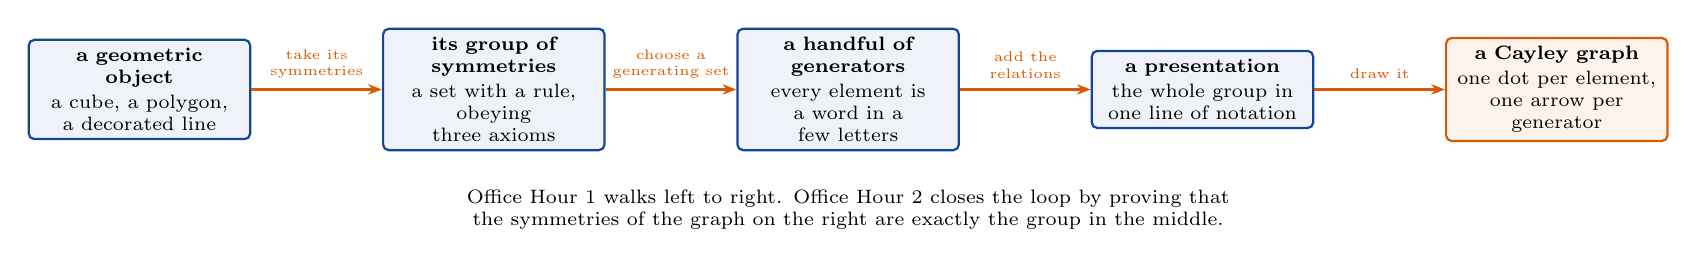
\begin{tikzpicture}[scale=1.0,>={Stealth[length=5pt]},font=\scriptsize]
  \node[draw=big,thick,rounded corners=2pt,fill=big!7,align=center,text width=74pt,inner sep=3pt] (N0) at (0,0) {\textbf{a geometric\\object}\\[1pt]a cube, a polygon,\\a decorated line};
  \node[draw=big,thick,rounded corners=2pt,fill=big!7,align=center,text width=74pt,inner sep=3pt] (N1) at (4.5,0) {\textbf{its group of\\symmetries}\\[1pt]a set with a rule,\\obeying three axioms};
  \node[draw=big,thick,rounded corners=2pt,fill=big!7,align=center,text width=74pt,inner sep=3pt] (N2) at (9.0,0) {\textbf{a handful of\\generators}\\[1pt]every element is\\a word in a few letters};
  \node[draw=big,thick,rounded corners=2pt,fill=big!7,align=center,text width=74pt,inner sep=3pt] (N3) at (13.5,0) {\textbf{a presentation}\\[1pt]the whole group in\\one line of notation};
  \node[draw=mkc,thick,rounded corners=2pt,fill=mkc!7,align=center,text width=74pt,inner sep=3pt] (N4) at (18.0,0) {\textbf{a Cayley graph}\\[1pt]one dot per element,\\one arrow per generator};
  \draw[->,very thick,mkc] (N0)--node[above,font=\tiny,mkc,align=center]{take its\\symmetries}(N1);
  \draw[->,very thick,mkc] (N1)--node[above,font=\tiny,mkc,align=center]{choose a\\generating set}(N2);
  \draw[->,very thick,mkc] (N2)--node[above,font=\tiny,mkc,align=center]{add the\\relations}(N3);
  \draw[->,very thick,mkc] (N3)--node[above,font=\tiny,mkc,align=center]{draw it}(N4);
  \node[font=\scriptsize,align=center,anchor=north,text width=470pt] at (9.0,-1.15) {Office Hour 1 walks left to right. Office Hour 2 closes the loop by proving that the symmetries of the graph on the right are exactly the group in the middle.};
\end{tikzpicture}
}\par\vspace{5pt}
\begin{minipage}[t]{238pt}\vspace{0pt}
{\sffamily\bfseries\color{big} Symmetry as a rigid motion}\par\vspace{1pt}
\emph{The gap it fills.} ``Symmetry'' is a feeling until you say exactly which motions count.\par\vspace{1pt}
\emph{What it buys.} A finite, countable, composable collection instead of a vague impression.\par\vspace{1pt}
\emph{Smallest example.} The cube has $24$ rotations, and you can check that number two independent ways: $8$ corners times $3$ turns, and $9+8+6+1$ by kind of axis. Two different countings agreeing is evidence the definition is the right one.\par\vspace{5pt}
{\sffamily\bfseries\color{big} The three axioms}\par\vspace{1pt}
\emph{The gap it fills.} Which collections deserve the name, and which facts hold for all of them at once.\par\vspace{1pt}
\emph{What it buys.} Everything provable without knowing a single element: the identity is unique, inverses are unique, $gx=k$ has exactly one solution, and $gx=gy$ forces $x=y$.\par\vspace{1pt}
\emph{Smallest example.} The six quarter turns of the cube are a natural-looking family, and they fail: two of them in a row give a corner turn. Without closure there is no group and none of the above applies.\par\vspace{5pt}
{\sffamily\bfseries\color{big} Isomorphism}\par\vspace{1pt}
\emph{The gap it fills.} Two groups built from unrelated material can be the same group.\par\vspace{1pt}
\emph{What it buys.} A dictionary. Every question about one becomes a question about the other, and you may work in whichever is easier.\par\vspace{1pt}
\emph{Smallest example.} The rotations of the cube are $S_4$. ``Which turn is this?'' becomes ``which permutation of four things is this?'', and the second question needs no spatial imagination at all.
\end{minipage}\hfill
\begin{minipage}[t]{238pt}\vspace{0pt}
{\sffamily\bfseries\color{big} Cycle notation}\par\vspace{1pt}
\emph{The gap it fills.} A permutation written as a list of images is unreadable and hopeless to multiply.\par\vspace{1pt}
\emph{What it buys.} A short normal form, and a multiplication you can carry out with a pencil in a few seconds.\par\vspace{1pt}
\emph{Smallest example.} $(2\,6)\cdot(1\,2\,4)(3\,5)=(1\,6\,2\,4)(3\,5)$, computed by pushing six numbers through two factors. Try describing the same product as two motions of a cube and the contrast is immediate.\par\vspace{5pt}
{\sffamily\bfseries\color{big} Generating sets}\par\vspace{1pt}
\emph{The gap it fills.} A group can be enormous or infinite, so listing it is not an option.\par\vspace{1pt}
\emph{What it buys.} The whole group described by a handful of elements, and a homomorphism out of it determined by where those few elements go.\par\vspace{1pt}
\emph{Smallest example.} Two reflections generate all ten symmetries of the pentagon; $n-1$ neighbour swaps generate all $n!$ permutations. In both cases a small list controls everything.\par\vspace{5pt}
{\sffamily\bfseries\color{big} Relations and presentations}\par\vspace{1pt}
\emph{The gap it fills.} Words in the generators are not unique, so you need to say which words are equal.\par\vspace{1pt}
\emph{What it buys.} An entire group compressed into one line, and a mechanical way to decide equality in favourable cases.\par\vspace{1pt}
\emph{Smallest example.} $\langle a,b \mid aba\inv b\inv\rangle$ is $\Z^2$. Delete that single relator and the same two generators give $F_2$, a completely different group. One line of notation is doing all the work.
\end{minipage}\hfill
\begin{minipage}[t]{238pt}\vspace{0pt}
{\sffamily\bfseries\color{big} The free group}\par\vspace{1pt}
\emph{The gap it fills.} What if you impose no relations at all?\par\vspace{1pt}
\emph{What it buys.} A universal source: every group is a free group with relations added, so free groups sit underneath the whole subject.\par\vspace{1pt}
\emph{Smallest example.} Within distance $k$ of the identity, $\Z^2$ has about $k^2$ elements and $F_2$ about $3^k$. Same number of generators, utterly different sizes, and the only difference is one relation.\par\vspace{5pt}
{\sffamily\bfseries\color{big} Homomorphism, kernel, quotient}\par\vspace{1pt}
\emph{The gap it fills.} Comparing two groups, and building smaller ones from larger ones.\par\vspace{1pt}
\emph{What it buys.} Structure-preserving maps, the first isomorphism theorem, and the meaning of the slash in $\Z/n\Z$.\par\vspace{1pt}
\emph{Smallest example.} The sign map $S_n\to\Z/2\Z$ turns a question about rearranging $n$ objects into a question about even and odd, which is the difference between a hard problem and an easy one.\par\vspace{5pt}
{\sffamily\bfseries\color{big} The Cayley graph}\par\vspace{1pt}
\emph{The gap it fills.} Algebra by itself gives nothing to look at.\par\vspace{1pt}
\emph{What it buys.} One dot per element, one coloured arrow per generator, and a picture in which words become paths and relations become loops.\par\vspace{1pt}
\emph{Smallest example.} The arrowed polygon, the arrowed line, the coloured grid and the four-valent tree are the same construction applied to $\Z/n\Z$, $\Z$, $\Z^2$ and $F_2$. All four appeared in this office hour before the name did.
\end{minipage}
\end{minipage}
}

% ================================================================ INTERLUDE Q (concept map)
\interlude{Q. The map of this office hour: how the ideas fit together}{
\begin{minipage}[t]{744pt}\vspace{0pt}
\small
Everything in Office Hour 1 is one journey with a loop at the end. You start with something you can hold, extract its symmetries, notice that the result obeys three rules, and then spend the rest of the chapter learning to describe, compare and finally redraw such a thing. Read the map along the orange arrows.\par\vspace{3pt}
\centerline{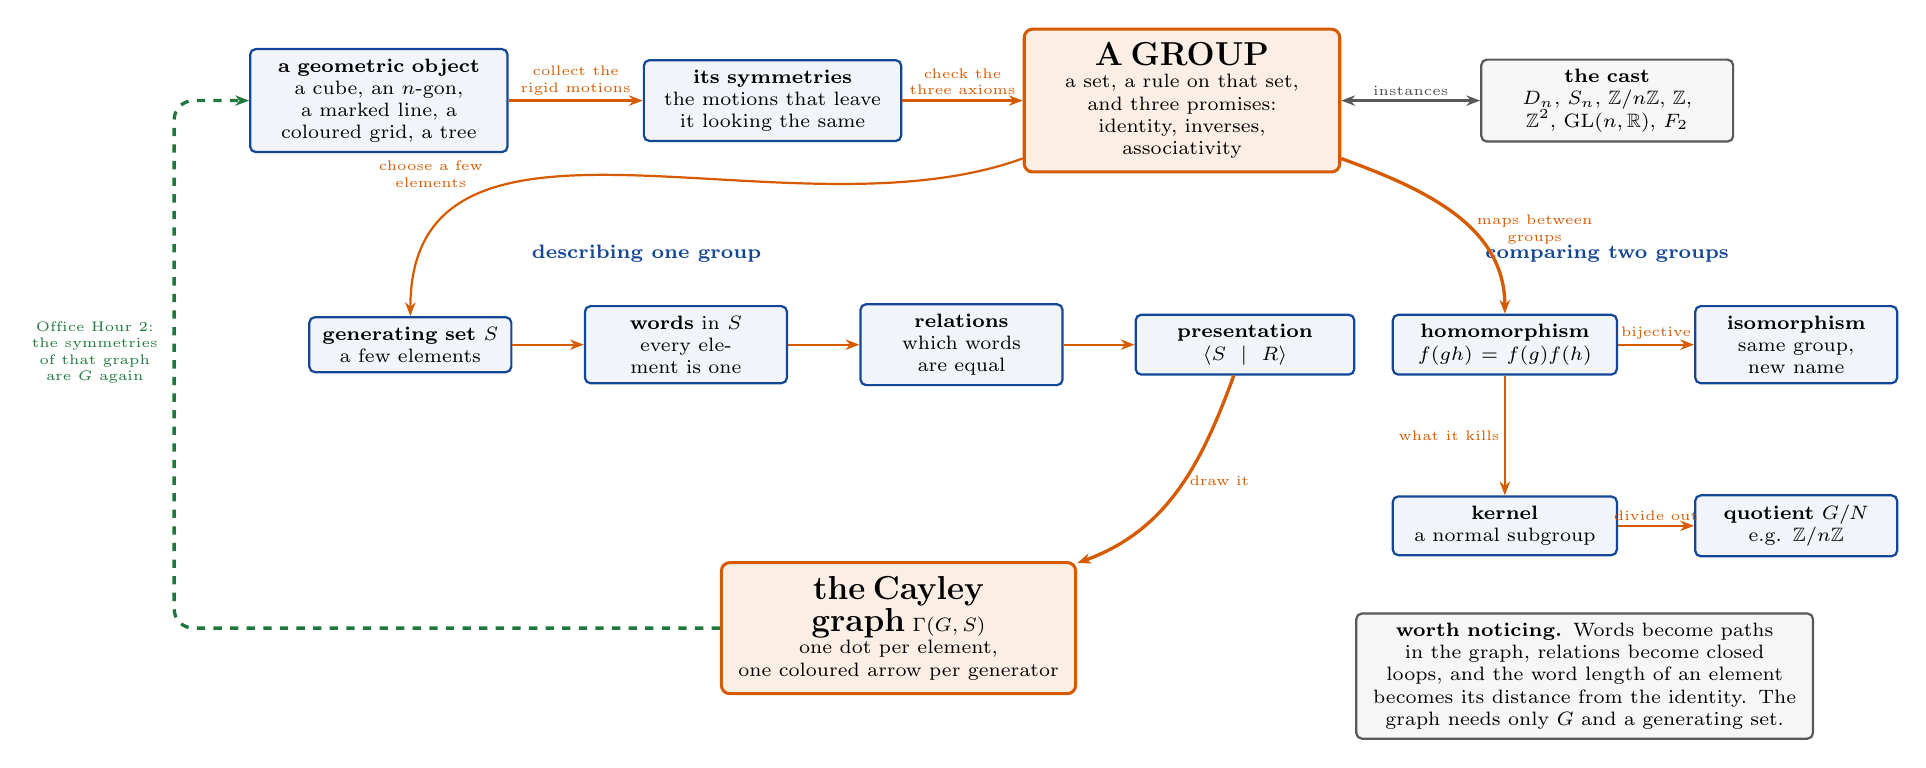
\begin{tikzpicture}[scale=1.0,font=\scriptsize,>={Stealth[length=5pt]},
  box/.style={draw=big,thick,rounded corners=2pt,fill=big!6,align=center,inner sep=3.5pt},
  hub/.style={draw=mkc,line width=1.1pt,rounded corners=3pt,fill=mkc!10,align=center,inner sep=5pt},
  ex/.style={draw=gray!70!black,thick,rounded corners=2pt,fill=gray!7,align=center,inner sep=3.5pt},
  lab/.style={font=\tiny,mkc,align=center,inner sep=1.5pt}]

% ---------- top band: the road in ----------
\node[box,text width=86pt] (obj) at (0,3.3) {\textbf{a geometric object}\\ a cube, an $n$-gon, a marked line, a coloured grid, a tree};
\node[box,text width=86pt] (sym) at (5.0,3.3) {\textbf{its symmetries}\\ the motions that leave it looking the same};
\node[hub,text width=104pt] (grp) at (10.2,3.3) {\textbf{\large A GROUP}\\ a set, a rule on that set,\\ and three promises:\\ identity, inverses, associativity};
\node[ex,text width=84pt] (exs) at (15.6,3.3) {\textbf{the cast}\\ $D_n$, $S_n$, $\Z/n\Z$, $\Z$, $\Z^2$, $\GL(n,\R)$, $F_2$};
\draw[->,very thick,mkc] (obj)--node[lab,above]{collect the\\rigid motions}(sym);
\draw[->,very thick,mkc] (sym)--node[lab,above]{check the\\three axioms}(grp);
\draw[<->,thick,gray!70!black] (grp)--node[lab,above,text=gray!60!black]{instances}(exs);

% ---------- left cluster: describing a group ----------
\node[font=\scriptsize\bfseries,color=big] at (3.4,1.35) {describing one group};
\node[box,text width=66pt] (gen) at (0.4,0.2) {\textbf{generating set} $S$\\ a few elements};
\node[box,text width=66pt] (wrd) at (3.9,0.2) {\textbf{words} in $S$\\ every element is one};
\node[box,text width=66pt] (rel) at (7.4,0.2) {\textbf{relations}\\ which words are equal};
\node[box,text width=72pt] (pre) at (11.0,0.2) {\textbf{presentation}\\ $\langle S \mid R\rangle$};
\draw[->,thick,mkc] (gen)--(wrd);
\draw[->,thick,mkc] (wrd)--(rel);
\draw[->,thick,mkc] (rel)--(pre);
\draw[->,thick,mkc] (grp) to[out=200,in=90] node[lab,above left,pos=0.72]{choose a few\\elements}(gen);

% ---------- right cluster: comparing groups ----------
\node[font=\scriptsize\bfseries,color=big] at (15.6,1.35) {comparing two groups};
\node[box,text width=74pt] (hom) at (14.3,0.2) {\textbf{homomorphism}\\ $f(gh)=f(g)f(h)$};
\node[box,text width=66pt] (iso) at (18.0,0.2) {\textbf{isomorphism}\\ same group,\\ new name};
\node[box,text width=74pt] (ker) at (14.3,-2.1) {\textbf{kernel}\\ a normal subgroup};
\node[box,text width=66pt] (quo) at (18.0,-2.1) {\textbf{quotient} $G/N$\\ e.g. $\Z/n\Z$};
\draw[->,thick,mkc] (hom)--node[lab,above]{bijective}(iso);
\draw[->,thick,mkc] (hom)--node[lab,left]{what it kills}(ker);
\draw[->,thick,mkc] (ker)--node[lab,above]{divide out}(quo);
\draw[->,very thick,mkc] (grp) to[out=340,in=90] node[lab,right,pos=0.6]{maps between\\groups}(hom);

% ---------- bottom: the road out ----------
\node[hub,text width=118pt] (cay) at (6.6,-3.4) {\textbf{\large the Cayley graph} $\Gamma(G,S)$\\ one dot per element,\\ one coloured arrow per generator};
\draw[->,very thick,mkc] (pre) to[out=250,in=20] node[lab,right,pos=0.45]{draw it}(cay);
\draw[->,very thick,dashed,why,rounded corners=7pt] (cay.west) -- (-2.6,-3.4) -- (-2.6,3.3) -- (obj.west);
\node[lab,text=why,align=center,anchor=east] at (-2.75,0.1) {Office Hour 2:\\the symmetries\\of that graph\\are $G$ again};

% ---------- notes ----------
\node[ex,text width=158pt,anchor=north west] at (12.4,-3.2) {\textbf{worth noticing.} Words become paths in the graph, relations become closed loops, and the word length of an element becomes its distance from the identity. The graph needs only $G$ and a generating set.};
\end{tikzpicture}}\par\vspace{4pt}
\begin{minipage}[t]{368pt}\vspace{0pt}
\begin{why}
\emph{Why the loop at the bottom matters.} The journey begins with a geometric object and produces a group. The dashed arrow says the journey can be run backwards: from the group alone you can build a graph, and the symmetries of that graph turn out to be the group you started from. That closes the circle, and it is the theorem Office Hour 2 proves. Until it is proved, ``a group is a collection of symmetries'' is only a slogan supported by examples.
\end{why}
\end{minipage}\hfill
\begin{minipage}[t]{360pt}\vspace{0pt}
\begin{bigpic}
The two clusters in the middle answer two different questions and it is worth keeping them apart. The left cluster asks \emph{how do I write this group down}, and its answer is a presentation. The right cluster asks \emph{how does this group compare with that one}, and its answers are the isomorphism theorems. The examples along the top are where both clusters are tested: every one of them appears with a generating set, a presentation, and at least one homomorphism.
\end{bigpic}
\end{minipage}
\end{minipage}
}

% ================================================================ BOOK p.6
\bookpage{021}{6}{
  \mk{1}{52}{70} \mk{2}{52}{227} \mk{3}{52}{485} \hl{67}{477}{330}{24}
  \mk{4}{52}{509} \mk{5}{52}{560}
}
\anncol{
\A{1}{``Do $h$, then do $g$'' is $gh$}
This right-to-left convention comes from writing functions on the left of their inputs: $(g\circ h)(x)=g(h(x))$, so $h$ acts first. The computations on page 7 depend on it.

\A{2}{The dihedral group $D_n$}
Now reflections \emph{are} allowed: a flat polygon lives in the plane, so you can lift it and flip it over.
Before the new vocabulary, run the three checks. Identity: leave the polygon alone. Inverses: turn a rotation back, and a reflection undoes itself. Associativity: free, because symmetries are functions and ``do $h$, then $g$'' is composition. Only then the extra facts: $D_n$ has $2n$ elements, $n$ rotations (multiples of $2\pi/n$, including the identity) and $n$ reflections; it is not abelian; the rotations form a subgroup.
(Some books call it $D_{2n}$, naming it by its size; this book names it by the polygon.)
\begin{lookahead}
Interlude L runs all three checks with before/after pictures of the pentagon, then lists the extra properties; Interlude D turns the ten symmetries into words in $s$ and $t$.
\end{lookahead}
In the book's figure $t$ is the reflection in the vertical axis and $s$ the one in the axis rotated by $\pi/5=36^\circ$ from it. For odd $n$ every axis runs through a vertex and the midpoint of the opposite edge.

\A{3}{``$s$ and $t$ generate $D_n$''}
A set $S$ \emph{generates} $G$ if every element of $G$ is a product of elements of $S$ and their inverses. This idea runs through the whole book; it is made formal in \S1.4.
\begin{why}
Reflecting in two lines that meet at angle $\theta$ is the same as rotating by $2\theta$ about their intersection. Here $\theta=\pi/n$, so $st$ is the rotation by $2\pi/n$: one ``click''. Hence $(st)^m$ is $m$ clicks, all $n$ rotations are $(st)^m$ for $m=0,\dots,n-1$, and every reflection is (rotation)$\cdot s$. So $s,t$ really do generate everything.
\end{why}

\A{4}{$s=s\inv$}
Reflecting twice returns everything to its place, so $s^2=1$: $s$ is its own inverse.

\A{5}{The symmetric group $S_n$}
The same three checks, now with no geometry to respect. Identity: leave every point where it is. Inverses: read the cycle backwards, or reverse every arrow. Associativity: free again, since the rule is composition of functions. So \emph{every} rearrangement counts, and $|S_n|=n!$; ``symmetries of $n$ points'' just means there are no distances or shape to preserve. Cube $=S_4$ says the rotations permute the four diagonals as freely as four loose points.
\begin{lookahead}
Interlude L checks the axioms for $S_n$ with tokens moving between slots, and collects what makes it interesting: size $n!$, not abelian, generated by neighbour swaps.
\end{lookahead}
}


% ================================================================ INTERLUDE L (page 6: D_n and S_n checked against the axioms)
\interlude{L. Page 6: the two new examples, first checked against the three axioms}{
\begin{minipage}[t]{744pt}\vspace{0pt}
\small
The book introduces $D_n$ and $S_n$ in a sentence each. It is worth doing slowly once: say what the \emph{set} is and what the \emph{rule} is, check the three promises, and only then collect the extra features. In the pictures, grey numbers are fixed positions or slots and a coloured disc names the original corner or token now sitting there.\par\vspace{4pt}
\begin{minipage}[t]{368pt}\vspace{0pt}
{\sffamily\bfseries\color{big} The dihedral group $D_5$ (the pentagon)}\par\vspace{2pt}
\emph{Set:} the $10$ rigid motions of a regular pentagon, $5$ rotations (by $0^\circ,72^\circ,\dots,288^\circ$) and $5$ reflections. \emph{Rule:} $gh$ means ``do $h$, then $g$'', as for the cube. Reflections count here because a flat polygon can be flipped over in space.\par\vspace{2pt}
{\sffamily\bfseries 0. Closure.} Two reflections in a row are not a reflection, but they are still a symmetry, so nothing leaves the set. The same picture shows the order matters.\par\nobreak\vspace{1pt}
\centerline{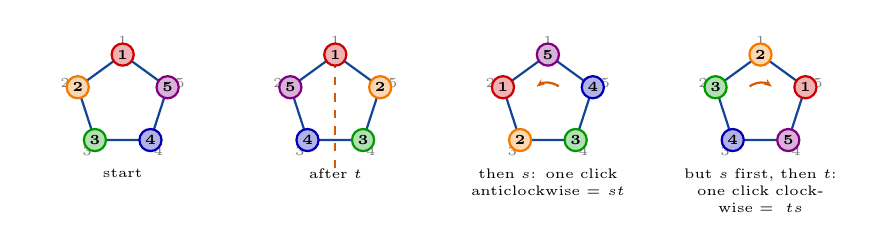
\begin{tikzpicture}[scale=0.6]
  \draw[thick,big] (0.000,1.000)--(-0.951,0.309)--(-0.588,-0.809)--(0.588,-0.809)--(0.951,0.309)--cycle;
  \node[font=\tiny,gray] at (0.000,1.280) {1};
  \node[font=\tiny\bfseries,circle,inner sep=0.3pt,minimum size=8pt,fill=red!80!black!30,draw=red!80!black,thick,text=black] at (0.000,1.000) {1};
  \node[font=\tiny,gray] at (-1.217,0.396) {2};
  \node[font=\tiny\bfseries,circle,inner sep=0.3pt,minimum size=8pt,fill=orange!95!black!30,draw=orange!95!black,thick,text=black] at (-0.951,0.309) {2};
  \node[font=\tiny,gray] at (-0.752,-1.036) {3};
  \node[font=\tiny\bfseries,circle,inner sep=0.3pt,minimum size=8pt,fill=green!60!black!30,draw=green!60!black,thick,text=black] at (-0.588,-0.809) {3};
  \node[font=\tiny,gray] at (0.752,-1.036) {4};
  \node[font=\tiny\bfseries,circle,inner sep=0.3pt,minimum size=8pt,fill=blue!70!black!30,draw=blue!70!black,thick,text=black] at (0.588,-0.809) {4};
  \node[font=\tiny,gray] at (1.217,0.396) {5};
  \node[font=\tiny\bfseries,circle,inner sep=0.3pt,minimum size=8pt,fill=violet!30,draw=violet,thick,text=black] at (0.951,0.309) {5};
  \node[font=\tiny,align=center,anchor=north,text width=62pt] at (0.000,-1.220) {start};
  \draw[thick,big] (4.500,1.000)--(3.549,0.309)--(3.912,-0.809)--(5.088,-0.809)--(5.451,0.309)--cycle;
  \draw[dashed,thick,mkc] (4.500,-1.400)--(4.500,1.400);
  \node[font=\tiny,gray] at (4.500,1.280) {1};
  \node[font=\tiny\bfseries,circle,inner sep=0.3pt,minimum size=8pt,fill=red!80!black!30,draw=red!80!black,thick,text=black] at (4.500,1.000) {1};
  \node[font=\tiny,gray] at (3.283,0.396) {2};
  \node[font=\tiny\bfseries,circle,inner sep=0.3pt,minimum size=8pt,fill=violet!30,draw=violet,thick,text=black] at (3.549,0.309) {5};
  \node[font=\tiny,gray] at (3.748,-1.036) {3};
  \node[font=\tiny\bfseries,circle,inner sep=0.3pt,minimum size=8pt,fill=blue!70!black!30,draw=blue!70!black,thick,text=black] at (3.912,-0.809) {4};
  \node[font=\tiny,gray] at (5.252,-1.036) {4};
  \node[font=\tiny\bfseries,circle,inner sep=0.3pt,minimum size=8pt,fill=green!60!black!30,draw=green!60!black,thick,text=black] at (5.088,-0.809) {3};
  \node[font=\tiny,gray] at (5.717,0.396) {5};
  \node[font=\tiny\bfseries,circle,inner sep=0.3pt,minimum size=8pt,fill=orange!95!black!30,draw=orange!95!black,thick,text=black] at (5.451,0.309) {2};
  \node[font=\tiny,align=center,anchor=north,text width=62pt] at (4.500,-1.220) {after $t$};
  \draw[thick,big] (9.000,1.000)--(8.049,0.309)--(8.412,-0.809)--(9.588,-0.809)--(9.951,0.309)--cycle;
  \draw[-{Stealth[length=3pt]},thick,mkc] (9.000,0.000)++(55:0.4) arc (55:127:0.4);
  \node[font=\tiny,gray] at (9.000,1.280) {1};
  \node[font=\tiny\bfseries,circle,inner sep=0.3pt,minimum size=8pt,fill=violet!30,draw=violet,thick,text=black] at (9.000,1.000) {5};
  \node[font=\tiny,gray] at (7.783,0.396) {2};
  \node[font=\tiny\bfseries,circle,inner sep=0.3pt,minimum size=8pt,fill=red!80!black!30,draw=red!80!black,thick,text=black] at (8.049,0.309) {1};
  \node[font=\tiny,gray] at (8.248,-1.036) {3};
  \node[font=\tiny\bfseries,circle,inner sep=0.3pt,minimum size=8pt,fill=orange!95!black!30,draw=orange!95!black,thick,text=black] at (8.412,-0.809) {2};
  \node[font=\tiny,gray] at (9.752,-1.036) {4};
  \node[font=\tiny\bfseries,circle,inner sep=0.3pt,minimum size=8pt,fill=green!60!black!30,draw=green!60!black,thick,text=black] at (9.588,-0.809) {3};
  \node[font=\tiny,gray] at (10.217,0.396) {5};
  \node[font=\tiny\bfseries,circle,inner sep=0.3pt,minimum size=8pt,fill=blue!70!black!30,draw=blue!70!black,thick,text=black] at (9.951,0.309) {4};
  \node[font=\tiny,align=center,anchor=north,text width=62pt] at (9.000,-1.220) {then $s$: one click\\anticlockwise $=st$};
  \draw[thick,big] (13.500,1.000)--(12.549,0.309)--(12.912,-0.809)--(14.088,-0.809)--(14.451,0.309)--cycle;
  \draw[-{Stealth[length=3pt]},thick,mkc] (13.500,0.000)++(125:0.4) arc (125:53:0.4);
  \node[font=\tiny,gray] at (13.500,1.280) {1};
  \node[font=\tiny\bfseries,circle,inner sep=0.3pt,minimum size=8pt,fill=orange!95!black!30,draw=orange!95!black,thick,text=black] at (13.500,1.000) {2};
  \node[font=\tiny,gray] at (12.283,0.396) {2};
  \node[font=\tiny\bfseries,circle,inner sep=0.3pt,minimum size=8pt,fill=green!60!black!30,draw=green!60!black,thick,text=black] at (12.549,0.309) {3};
  \node[font=\tiny,gray] at (12.748,-1.036) {3};
  \node[font=\tiny\bfseries,circle,inner sep=0.3pt,minimum size=8pt,fill=blue!70!black!30,draw=blue!70!black,thick,text=black] at (12.912,-0.809) {4};
  \node[font=\tiny,gray] at (14.252,-1.036) {4};
  \node[font=\tiny\bfseries,circle,inner sep=0.3pt,minimum size=8pt,fill=violet!30,draw=violet,thick,text=black] at (14.088,-0.809) {5};
  \node[font=\tiny,gray] at (14.717,0.396) {5};
  \node[font=\tiny\bfseries,circle,inner sep=0.3pt,minimum size=8pt,fill=red!80!black!30,draw=red!80!black,thick,text=black] at (14.451,0.309) {1};
  \node[font=\tiny,align=center,anchor=north,text width=62pt] at (13.500,-1.220) {but $s$ first, then $t$:\\one click clockwise $=ts$};
\end{tikzpicture}
}\par\vspace{2pt}
{\sffamily\bfseries 1. Identity.} ``Leave the pentagon alone'' is the rotation by $0^\circ$; before or after any move it changes nothing.\par\nobreak\vspace{1pt}
\centerline{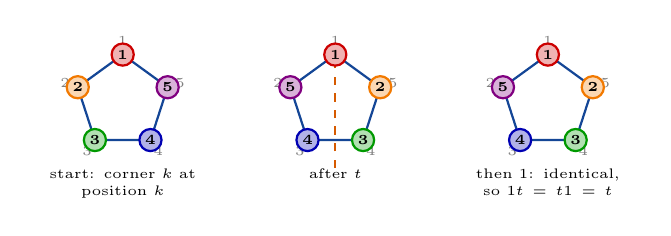
\begin{tikzpicture}[scale=0.6]
  \draw[thick,big] (0.000,1.000)--(-0.951,0.309)--(-0.588,-0.809)--(0.588,-0.809)--(0.951,0.309)--cycle;
  \node[font=\tiny,gray] at (0.000,1.280) {1};
  \node[font=\tiny\bfseries,circle,inner sep=0.3pt,minimum size=8pt,fill=red!80!black!30,draw=red!80!black,thick,text=black] at (0.000,1.000) {1};
  \node[font=\tiny,gray] at (-1.217,0.396) {2};
  \node[font=\tiny\bfseries,circle,inner sep=0.3pt,minimum size=8pt,fill=orange!95!black!30,draw=orange!95!black,thick,text=black] at (-0.951,0.309) {2};
  \node[font=\tiny,gray] at (-0.752,-1.036) {3};
  \node[font=\tiny\bfseries,circle,inner sep=0.3pt,minimum size=8pt,fill=green!60!black!30,draw=green!60!black,thick,text=black] at (-0.588,-0.809) {3};
  \node[font=\tiny,gray] at (0.752,-1.036) {4};
  \node[font=\tiny\bfseries,circle,inner sep=0.3pt,minimum size=8pt,fill=blue!70!black!30,draw=blue!70!black,thick,text=black] at (0.588,-0.809) {4};
  \node[font=\tiny,gray] at (1.217,0.396) {5};
  \node[font=\tiny\bfseries,circle,inner sep=0.3pt,minimum size=8pt,fill=violet!30,draw=violet,thick,text=black] at (0.951,0.309) {5};
  \node[font=\tiny,align=center,anchor=north,text width=62pt] at (0.000,-1.220) {start: corner $k$ at\\position $k$};
  \draw[thick,big] (4.500,1.000)--(3.549,0.309)--(3.912,-0.809)--(5.088,-0.809)--(5.451,0.309)--cycle;
  \draw[dashed,thick,mkc] (4.500,-1.400)--(4.500,1.400);
  \node[font=\tiny,gray] at (4.500,1.280) {1};
  \node[font=\tiny\bfseries,circle,inner sep=0.3pt,minimum size=8pt,fill=red!80!black!30,draw=red!80!black,thick,text=black] at (4.500,1.000) {1};
  \node[font=\tiny,gray] at (3.283,0.396) {2};
  \node[font=\tiny\bfseries,circle,inner sep=0.3pt,minimum size=8pt,fill=violet!30,draw=violet,thick,text=black] at (3.549,0.309) {5};
  \node[font=\tiny,gray] at (3.748,-1.036) {3};
  \node[font=\tiny\bfseries,circle,inner sep=0.3pt,minimum size=8pt,fill=blue!70!black!30,draw=blue!70!black,thick,text=black] at (3.912,-0.809) {4};
  \node[font=\tiny,gray] at (5.252,-1.036) {4};
  \node[font=\tiny\bfseries,circle,inner sep=0.3pt,minimum size=8pt,fill=green!60!black!30,draw=green!60!black,thick,text=black] at (5.088,-0.809) {3};
  \node[font=\tiny,gray] at (5.717,0.396) {5};
  \node[font=\tiny\bfseries,circle,inner sep=0.3pt,minimum size=8pt,fill=orange!95!black!30,draw=orange!95!black,thick,text=black] at (5.451,0.309) {2};
  \node[font=\tiny,align=center,anchor=north,text width=62pt] at (4.500,-1.220) {after $t$};
  \draw[thick,big] (9.000,1.000)--(8.049,0.309)--(8.412,-0.809)--(9.588,-0.809)--(9.951,0.309)--cycle;
  \node[font=\tiny,gray] at (9.000,1.280) {1};
  \node[font=\tiny\bfseries,circle,inner sep=0.3pt,minimum size=8pt,fill=red!80!black!30,draw=red!80!black,thick,text=black] at (9.000,1.000) {1};
  \node[font=\tiny,gray] at (7.783,0.396) {2};
  \node[font=\tiny\bfseries,circle,inner sep=0.3pt,minimum size=8pt,fill=violet!30,draw=violet,thick,text=black] at (8.049,0.309) {5};
  \node[font=\tiny,gray] at (8.248,-1.036) {3};
  \node[font=\tiny\bfseries,circle,inner sep=0.3pt,minimum size=8pt,fill=blue!70!black!30,draw=blue!70!black,thick,text=black] at (8.412,-0.809) {4};
  \node[font=\tiny,gray] at (9.752,-1.036) {4};
  \node[font=\tiny\bfseries,circle,inner sep=0.3pt,minimum size=8pt,fill=green!60!black!30,draw=green!60!black,thick,text=black] at (9.588,-0.809) {3};
  \node[font=\tiny,gray] at (10.217,0.396) {5};
  \node[font=\tiny\bfseries,circle,inner sep=0.3pt,minimum size=8pt,fill=orange!95!black!30,draw=orange!95!black,thick,text=black] at (9.951,0.309) {2};
  \node[font=\tiny,align=center,anchor=north,text width=62pt] at (9.000,-1.220) {then $1$: identical,\\so $1t=t1=t$};
\end{tikzpicture}
}\par\vspace{2pt}
{\sffamily\bfseries 2. Inverses.} A rotation is undone by turning back, which is the same as turning forward the rest of the way. A reflection is its own inverse: apply $t$ twice and the second picture above is undone, $t^2=1$.\par\nobreak\vspace{1pt}
\centerline{\begin{tikzpicture}[scale=0.6]
  \draw[thick,big] (0.000,1.000)--(-0.951,0.309)--(-0.588,-0.809)--(0.588,-0.809)--(0.951,0.309)--cycle;
  \node[font=\tiny,gray] at (0.000,1.280) {1};
  \node[font=\tiny\bfseries,circle,inner sep=0.3pt,minimum size=8pt,fill=red!80!black!30,draw=red!80!black,thick,text=black] at (0.000,1.000) {1};
  \node[font=\tiny,gray] at (-1.217,0.396) {2};
  \node[font=\tiny\bfseries,circle,inner sep=0.3pt,minimum size=8pt,fill=orange!95!black!30,draw=orange!95!black,thick,text=black] at (-0.951,0.309) {2};
  \node[font=\tiny,gray] at (-0.752,-1.036) {3};
  \node[font=\tiny\bfseries,circle,inner sep=0.3pt,minimum size=8pt,fill=green!60!black!30,draw=green!60!black,thick,text=black] at (-0.588,-0.809) {3};
  \node[font=\tiny,gray] at (0.752,-1.036) {4};
  \node[font=\tiny\bfseries,circle,inner sep=0.3pt,minimum size=8pt,fill=blue!70!black!30,draw=blue!70!black,thick,text=black] at (0.588,-0.809) {4};
  \node[font=\tiny,gray] at (1.217,0.396) {5};
  \node[font=\tiny\bfseries,circle,inner sep=0.3pt,minimum size=8pt,fill=violet!30,draw=violet,thick,text=black] at (0.951,0.309) {5};
  \node[font=\tiny,align=center,anchor=north,text width=62pt] at (0.000,-1.220) {start};
  \draw[thick,big] (4.500,1.000)--(3.549,0.309)--(3.912,-0.809)--(5.088,-0.809)--(5.451,0.309)--cycle;
  \draw[-{Stealth[length=3pt]},thick,mkc] (4.500,0.000)++(55:0.4) arc (55:127:0.4);
  \node[font=\tiny,gray] at (4.500,1.280) {1};
  \node[font=\tiny\bfseries,circle,inner sep=0.3pt,minimum size=8pt,fill=violet!30,draw=violet,thick,text=black] at (4.500,1.000) {5};
  \node[font=\tiny,gray] at (3.283,0.396) {2};
  \node[font=\tiny\bfseries,circle,inner sep=0.3pt,minimum size=8pt,fill=red!80!black!30,draw=red!80!black,thick,text=black] at (3.549,0.309) {1};
  \node[font=\tiny,gray] at (3.748,-1.036) {3};
  \node[font=\tiny\bfseries,circle,inner sep=0.3pt,minimum size=8pt,fill=orange!95!black!30,draw=orange!95!black,thick,text=black] at (3.912,-0.809) {2};
  \node[font=\tiny,gray] at (5.252,-1.036) {4};
  \node[font=\tiny\bfseries,circle,inner sep=0.3pt,minimum size=8pt,fill=green!60!black!30,draw=green!60!black,thick,text=black] at (5.088,-0.809) {3};
  \node[font=\tiny,gray] at (5.717,0.396) {5};
  \node[font=\tiny\bfseries,circle,inner sep=0.3pt,minimum size=8pt,fill=blue!70!black!30,draw=blue!70!black,thick,text=black] at (5.451,0.309) {4};
  \node[font=\tiny,align=center,anchor=north,text width=62pt] at (4.500,-1.220) {after one click $st$};
  \draw[thick,big] (9.000,1.000)--(8.049,0.309)--(8.412,-0.809)--(9.588,-0.809)--(9.951,0.309)--cycle;
  \draw[-{Stealth[length=3pt]},thick,mkc] (9.000,0.000)++(55:0.4) arc (55:343:0.4);
  \node[font=\tiny,gray] at (9.000,1.280) {1};
  \node[font=\tiny\bfseries,circle,inner sep=0.3pt,minimum size=8pt,fill=red!80!black!30,draw=red!80!black,thick,text=black] at (9.000,1.000) {1};
  \node[font=\tiny,gray] at (7.783,0.396) {2};
  \node[font=\tiny\bfseries,circle,inner sep=0.3pt,minimum size=8pt,fill=orange!95!black!30,draw=orange!95!black,thick,text=black] at (8.049,0.309) {2};
  \node[font=\tiny,gray] at (8.248,-1.036) {3};
  \node[font=\tiny\bfseries,circle,inner sep=0.3pt,minimum size=8pt,fill=green!60!black!30,draw=green!60!black,thick,text=black] at (8.412,-0.809) {3};
  \node[font=\tiny,gray] at (9.752,-1.036) {4};
  \node[font=\tiny\bfseries,circle,inner sep=0.3pt,minimum size=8pt,fill=blue!70!black!30,draw=blue!70!black,thick,text=black] at (9.588,-0.809) {4};
  \node[font=\tiny,gray] at (10.217,0.396) {5};
  \node[font=\tiny\bfseries,circle,inner sep=0.3pt,minimum size=8pt,fill=violet!30,draw=violet,thick,text=black] at (9.951,0.309) {5};
  \node[font=\tiny,align=center,anchor=north,text width=62pt] at (9.000,-1.220) {then $(st)^4$: home,\\so $(st)^{-1}=(st)^4$};
\end{tikzpicture}
}\par\vspace{2pt}
{\sffamily\bfseries 3. Associativity.} Free of charge: each symmetry is a function from the pentagon to itself, and $\big((fg)h\big)(x)=f\big(g(h(x))\big)=\big(f(gh)\big)(x)$ for every point $x$. So a word like $tst$ has one meaning.\par\vspace{2pt}
\begin{bigpic}
\textbf{Now the extra properties.} $|D_n|=2n$. Not abelian for $n\ge3$: the first picture shows $st\neq ts$. The reflections $s,t$ \emph{generate} it, since $st$ is one click: $(st)^m$ gives all $n$ rotations and $s(st)^m$ all $n$ reflections (Interlude D lists the ten words). The rotations alone form a subgroup, a copy of $\Z/n\Z$. The relations $s^2=t^2=1$ and $(st)^n=1$ pin the group down completely, which is the Coxeter idea named in the last line of the page.
\end{bigpic}
\end{minipage}\hfill
\begin{minipage}[t]{360pt}\vspace{0pt}
{\sffamily\bfseries\color{big} The symmetric group $S_n$ (permutations)}\par\vspace{2pt}
\emph{Set:} all bijections $\{1,\dots,n\}\to\{1,\dots,n\}$, that is, all ways of rearranging $n$ tokens among $n$ slots. \emph{Rule:} composition, $\tau\sigma$ meaning ``do $\sigma$, then $\tau$''. Nothing geometric has to be respected, which is why \emph{every} rearrangement is allowed.\par\vspace{2pt}
{\sffamily\bfseries 0. Closure.} A rearrangement followed by a rearrangement is a rearrangement: every slot still ends up with exactly one token.\par\nobreak\vspace{1pt}
\centerline{\begin{tikzpicture}[scale=0.5]
  \node[font=\scriptsize,gray] at (1.35,0.6) {slot 1};
  \node[font=\scriptsize,gray] at (2.70,0.6) {slot 2};
  \node[font=\scriptsize,gray] at (4.05,0.6) {slot 3};
  \node[font=\scriptsize,gray] at (5.40,0.6) {slot 4};
  \node[font=\scriptsize\bfseries,circle,inner sep=1pt,minimum size=11pt,fill=red!80!black!30,draw=red!80!black,thick,text=black] at (1.35,0.00) {1};
  \node[font=\scriptsize\bfseries,circle,inner sep=1pt,minimum size=11pt,fill=orange!95!black!30,draw=orange!95!black,thick,text=black] at (2.70,0.00) {2};
  \node[font=\scriptsize\bfseries,circle,inner sep=1pt,minimum size=11pt,fill=green!60!black!30,draw=green!60!black,thick,text=black] at (4.05,0.00) {3};
  \node[font=\scriptsize\bfseries,circle,inner sep=1pt,minimum size=11pt,fill=blue!70!black!30,draw=blue!70!black,thick,text=black] at (5.40,0.00) {4};
  \node[font=\scriptsize,anchor=west,align=left] at (5.90,0.00) {start: token $k$ in slot $k$};
  \draw[thick,red!80!black] (1.35,-0.30) .. controls (1.35,-0.90) and (2.70,-1.20) .. (2.70,-1.80);
  \draw[thick,orange!95!black] (2.70,-0.30) .. controls (2.70,-0.90) and (4.05,-1.20) .. (4.05,-1.80);
  \draw[thick,green!60!black] (4.05,-0.30) .. controls (4.05,-0.90) and (1.35,-1.20) .. (1.35,-1.80);
  \draw[thick,blue!70!black] (5.40,-0.30) .. controls (5.40,-0.90) and (5.40,-1.20) .. (5.40,-1.80);
  \node[font=\scriptsize\bfseries,circle,inner sep=1pt,minimum size=11pt,fill=green!60!black!30,draw=green!60!black,thick,text=black] at (1.35,-2.10) {3};
  \node[font=\scriptsize\bfseries,circle,inner sep=1pt,minimum size=11pt,fill=red!80!black!30,draw=red!80!black,thick,text=black] at (2.70,-2.10) {1};
  \node[font=\scriptsize\bfseries,circle,inner sep=1pt,minimum size=11pt,fill=orange!95!black!30,draw=orange!95!black,thick,text=black] at (4.05,-2.10) {2};
  \node[font=\scriptsize\bfseries,circle,inner sep=1pt,minimum size=11pt,fill=blue!70!black!30,draw=blue!70!black,thick,text=black] at (5.40,-2.10) {4};
  \node[font=\scriptsize,anchor=west,align=left] at (5.90,-2.10) {after $\sigma=(1\,2\,3)$};
  \draw[thick,green!60!black] (1.35,-2.40) .. controls (1.35,-3.00) and (1.35,-3.30) .. (1.35,-3.90);
  \draw[thick,red!80!black] (2.70,-2.40) .. controls (2.70,-3.00) and (2.70,-3.30) .. (2.70,-3.90);
  \draw[thick,orange!95!black] (4.05,-2.40) .. controls (4.05,-3.00) and (5.40,-3.30) .. (5.40,-3.90);
  \draw[thick,blue!70!black] (5.40,-2.40) .. controls (5.40,-3.00) and (4.05,-3.30) .. (4.05,-3.90);
  \node[font=\scriptsize\bfseries,circle,inner sep=1pt,minimum size=11pt,fill=green!60!black!30,draw=green!60!black,thick,text=black] at (1.35,-4.20) {3};
  \node[font=\scriptsize\bfseries,circle,inner sep=1pt,minimum size=11pt,fill=red!80!black!30,draw=red!80!black,thick,text=black] at (2.70,-4.20) {1};
  \node[font=\scriptsize\bfseries,circle,inner sep=1pt,minimum size=11pt,fill=blue!70!black!30,draw=blue!70!black,thick,text=black] at (4.05,-4.20) {4};
  \node[font=\scriptsize\bfseries,circle,inner sep=1pt,minimum size=11pt,fill=orange!95!black!30,draw=orange!95!black,thick,text=black] at (5.40,-4.20) {2};
  \node[font=\scriptsize,anchor=west,align=left] at (5.90,-4.20) {then $\tau=(3\,4)$: net $\tau\sigma=(1\,2\,4\,3)$, again a\\rearrangement, so the set is closed};
\end{tikzpicture}
}\par\vspace{3pt}
{\sffamily\bfseries 1. Identity and 2. inverses, in one picture.} The identity is the permutation fixing every slot, written $1$ or $()$. The inverse is the cycle read backwards, or the loop picture of page 7 with every arrow reversed; the tokens retrace their strands.\par\nobreak\vspace{1pt}
\centerline{\begin{tikzpicture}[scale=0.5]
  \node[font=\scriptsize,gray] at (1.35,0.6) {slot 1};
  \node[font=\scriptsize,gray] at (2.70,0.6) {slot 2};
  \node[font=\scriptsize,gray] at (4.05,0.6) {slot 3};
  \node[font=\scriptsize,gray] at (5.40,0.6) {slot 4};
  \node[font=\scriptsize\bfseries,circle,inner sep=1pt,minimum size=11pt,fill=red!80!black!30,draw=red!80!black,thick,text=black] at (1.35,0.00) {1};
  \node[font=\scriptsize\bfseries,circle,inner sep=1pt,minimum size=11pt,fill=orange!95!black!30,draw=orange!95!black,thick,text=black] at (2.70,0.00) {2};
  \node[font=\scriptsize\bfseries,circle,inner sep=1pt,minimum size=11pt,fill=green!60!black!30,draw=green!60!black,thick,text=black] at (4.05,0.00) {3};
  \node[font=\scriptsize\bfseries,circle,inner sep=1pt,minimum size=11pt,fill=blue!70!black!30,draw=blue!70!black,thick,text=black] at (5.40,0.00) {4};
  \node[font=\scriptsize,anchor=west,align=left] at (5.90,0.00) {start};
  \draw[thick,red!80!black] (1.35,-0.30) .. controls (1.35,-0.90) and (2.70,-1.20) .. (2.70,-1.80);
  \draw[thick,orange!95!black] (2.70,-0.30) .. controls (2.70,-0.90) and (4.05,-1.20) .. (4.05,-1.80);
  \draw[thick,green!60!black] (4.05,-0.30) .. controls (4.05,-0.90) and (1.35,-1.20) .. (1.35,-1.80);
  \draw[thick,blue!70!black] (5.40,-0.30) .. controls (5.40,-0.90) and (5.40,-1.20) .. (5.40,-1.80);
  \node[font=\scriptsize\bfseries,circle,inner sep=1pt,minimum size=11pt,fill=green!60!black!30,draw=green!60!black,thick,text=black] at (1.35,-2.10) {3};
  \node[font=\scriptsize\bfseries,circle,inner sep=1pt,minimum size=11pt,fill=red!80!black!30,draw=red!80!black,thick,text=black] at (2.70,-2.10) {1};
  \node[font=\scriptsize\bfseries,circle,inner sep=1pt,minimum size=11pt,fill=orange!95!black!30,draw=orange!95!black,thick,text=black] at (4.05,-2.10) {2};
  \node[font=\scriptsize\bfseries,circle,inner sep=1pt,minimum size=11pt,fill=blue!70!black!30,draw=blue!70!black,thick,text=black] at (5.40,-2.10) {4};
  \node[font=\scriptsize,anchor=west,align=left] at (5.90,-2.10) {after $\sigma=(1\,2\,3)$};
  \draw[thick,green!60!black] (1.35,-2.40) .. controls (1.35,-3.00) and (1.35,-3.30) .. (1.35,-3.90);
  \draw[thick,red!80!black] (2.70,-2.40) .. controls (2.70,-3.00) and (2.70,-3.30) .. (2.70,-3.90);
  \draw[thick,orange!95!black] (4.05,-2.40) .. controls (4.05,-3.00) and (4.05,-3.30) .. (4.05,-3.90);
  \draw[thick,blue!70!black] (5.40,-2.40) .. controls (5.40,-3.00) and (5.40,-3.30) .. (5.40,-3.90);
  \node[font=\scriptsize\bfseries,circle,inner sep=1pt,minimum size=11pt,fill=green!60!black!30,draw=green!60!black,thick,text=black] at (1.35,-4.20) {3};
  \node[font=\scriptsize\bfseries,circle,inner sep=1pt,minimum size=11pt,fill=red!80!black!30,draw=red!80!black,thick,text=black] at (2.70,-4.20) {1};
  \node[font=\scriptsize\bfseries,circle,inner sep=1pt,minimum size=11pt,fill=orange!95!black!30,draw=orange!95!black,thick,text=black] at (4.05,-4.20) {2};
  \node[font=\scriptsize\bfseries,circle,inner sep=1pt,minimum size=11pt,fill=blue!70!black!30,draw=blue!70!black,thick,text=black] at (5.40,-4.20) {4};
  \node[font=\scriptsize,anchor=west,align=left] at (5.90,-4.20) {then $1=()$: row unchanged, so $1\sigma=\sigma$};
  \draw[thick,green!60!black] (1.35,-4.50) .. controls (1.35,-5.10) and (4.05,-5.40) .. (4.05,-6.00);
  \draw[thick,red!80!black] (2.70,-4.50) .. controls (2.70,-5.10) and (1.35,-5.40) .. (1.35,-6.00);
  \draw[thick,orange!95!black] (4.05,-4.50) .. controls (4.05,-5.10) and (2.70,-5.40) .. (2.70,-6.00);
  \draw[thick,blue!70!black] (5.40,-4.50) .. controls (5.40,-5.10) and (5.40,-5.40) .. (5.40,-6.00);
  \node[font=\scriptsize\bfseries,circle,inner sep=1pt,minimum size=11pt,fill=red!80!black!30,draw=red!80!black,thick,text=black] at (1.35,-6.30) {1};
  \node[font=\scriptsize\bfseries,circle,inner sep=1pt,minimum size=11pt,fill=orange!95!black!30,draw=orange!95!black,thick,text=black] at (2.70,-6.30) {2};
  \node[font=\scriptsize\bfseries,circle,inner sep=1pt,minimum size=11pt,fill=green!60!black!30,draw=green!60!black,thick,text=black] at (4.05,-6.30) {3};
  \node[font=\scriptsize\bfseries,circle,inner sep=1pt,minimum size=11pt,fill=blue!70!black!30,draw=blue!70!black,thick,text=black] at (5.40,-6.30) {4};
  \node[font=\scriptsize,anchor=west,align=left] at (5.90,-6.30) {instead, then $\sigma^{-1}=(1\,3\,2)$: every token home,\\so $\sigma^{-1}\sigma=1$};
\end{tikzpicture}
}\par\vspace{3pt}
{\sffamily\bfseries 3. Associativity.} Again free: for any $x$, both $(fg)h$ and $f(gh)$ send $x$ to $f(g(h(x)))$. That is why the book can say ``multiplication is composition of functions'' and stop. Only groups given by a \emph{formula}, like $\Z/n\Z$ on page 8, or by \emph{words}, like the free group on page 12, make you work for this axiom.\par\vspace{2pt}
\begin{bigpic}
\textbf{Now the extra properties.} $|S_n|=n!$: the token in slot 1 has $n$ choices, the next $n-1$, and so on. Not abelian for $n\ge3$, since $(1\,2)(2\,3)=(1\,2\,3)$ but $(2\,3)(1\,2)=(1\,3\,2)$. It is generated by the neighbour swaps $(1\,2),(2\,3),\dots$, which is exactly what the strand diagrams of page 8 draw. And $S_4$ is the rotation group of the cube (page 4, Interlude B2), so this abstract group has a geometric life too.
\end{bigpic}
\begin{tryit}
For $D_5$: which word is the reflection whose axis passes through position 3? Do the five rotations alone satisfy all three axioms? Do the five reflections alone? For $S_4$: compose $(1\,2\,3\,4)$ with itself, and invert $(1\,2)(3\,4)$.
\end{tryit}
\end{minipage}
\end{minipage}
}

% ================================================================ INTERLUDE D (page 6: s, t and the words they generate)
\interlude{D. Page 6 in a table: the ten symmetries of the pentagon as words in $s$ and $t$}{
\begin{minipage}[t]{744pt}\vspace{0pt}
\small
Take the pentagon with corners numbered $1$ to $5$ anticlockwise from the top, $t$ = reflection in the vertical axis (through corner 1) and $s$ = reflection in the axis rotated from it by $\pi/5=36^\circ$ (through the midpoint of edge $12$ and corner $4$), as in the book's figure. Every symmetry of the pentagon is one of the ten words below, and the picture shows where each word sends the numbered corners. Products are read right to left: $st$ means ``do $t$, then $s$''.\par\vspace{6pt}
\centering
\begin{tikzpicture}[scale=0.92]
\begin{scope}[shift={(0.0,0)}]
  \draw[thick,big] (90:1)--(162:1)--(234:1)--(306:1)--(18:1)--cycle;
  \node[font=\scriptsize,fill=white,inner sep=1pt,circle,draw=gray!60] at (90:1) {1};
  \node[font=\scriptsize,fill=white,inner sep=1pt,circle,draw=gray!60] at (162:1) {2};
  \node[font=\scriptsize,fill=white,inner sep=1pt,circle,draw=gray!60] at (234:1) {3};
  \node[font=\scriptsize,fill=white,inner sep=1pt,circle,draw=gray!60] at (306:1) {4};
  \node[font=\scriptsize,fill=white,inner sep=1pt,circle,draw=gray!60] at (378:1) {5};
  \node[font=\scriptsize,align=center] at (0,-1.55) {$1$};
\end{scope}
\begin{scope}[shift={(3.2,0)}]
  \draw[thick,big] (90:1)--(162:1)--(234:1)--(306:1)--(18:1)--cycle;
  \draw[-{Stealth[length=3pt]},mkc,thick] (0.35,0) arc (0:250:0.35);
  \node[font=\scriptsize,fill=white,inner sep=1pt,circle,draw=gray!60] at (162:1) {1};
  \node[font=\scriptsize,fill=white,inner sep=1pt,circle,draw=gray!60] at (234:1) {2};
  \node[font=\scriptsize,fill=white,inner sep=1pt,circle,draw=gray!60] at (306:1) {3};
  \node[font=\scriptsize,fill=white,inner sep=1pt,circle,draw=gray!60] at (378:1) {4};
  \node[font=\scriptsize,fill=white,inner sep=1pt,circle,draw=gray!60] at (90:1) {5};
  \node[font=\scriptsize,align=center] at (0,-1.55) {$st$};
\end{scope}
\begin{scope}[shift={(6.4,0)}]
  \draw[thick,big] (90:1)--(162:1)--(234:1)--(306:1)--(18:1)--cycle;
  \draw[-{Stealth[length=3pt]},mkc,thick] (0.35,0) arc (0:250:0.35);
  \node[font=\scriptsize,fill=white,inner sep=1pt,circle,draw=gray!60] at (234:1) {1};
  \node[font=\scriptsize,fill=white,inner sep=1pt,circle,draw=gray!60] at (306:1) {2};
  \node[font=\scriptsize,fill=white,inner sep=1pt,circle,draw=gray!60] at (378:1) {3};
  \node[font=\scriptsize,fill=white,inner sep=1pt,circle,draw=gray!60] at (90:1) {4};
  \node[font=\scriptsize,fill=white,inner sep=1pt,circle,draw=gray!60] at (162:1) {5};
  \node[font=\scriptsize,align=center] at (0,-1.55) {$(st)^2$};
\end{scope}
\begin{scope}[shift={(9.600000000000001,0)}]
  \draw[thick,big] (90:1)--(162:1)--(234:1)--(306:1)--(18:1)--cycle;
  \draw[-{Stealth[length=3pt]},mkc,thick] (0.35,0) arc (0:250:0.35);
  \node[font=\scriptsize,fill=white,inner sep=1pt,circle,draw=gray!60] at (306:1) {1};
  \node[font=\scriptsize,fill=white,inner sep=1pt,circle,draw=gray!60] at (378:1) {2};
  \node[font=\scriptsize,fill=white,inner sep=1pt,circle,draw=gray!60] at (90:1) {3};
  \node[font=\scriptsize,fill=white,inner sep=1pt,circle,draw=gray!60] at (162:1) {4};
  \node[font=\scriptsize,fill=white,inner sep=1pt,circle,draw=gray!60] at (234:1) {5};
  \node[font=\scriptsize,align=center] at (0,-1.55) {$(st)^3$};
\end{scope}
\begin{scope}[shift={(12.8,0)}]
  \draw[thick,big] (90:1)--(162:1)--(234:1)--(306:1)--(18:1)--cycle;
  \draw[-{Stealth[length=3pt]},mkc,thick] (0.35,0) arc (0:250:0.35);
  \node[font=\scriptsize,fill=white,inner sep=1pt,circle,draw=gray!60] at (378:1) {1};
  \node[font=\scriptsize,fill=white,inner sep=1pt,circle,draw=gray!60] at (90:1) {2};
  \node[font=\scriptsize,fill=white,inner sep=1pt,circle,draw=gray!60] at (162:1) {3};
  \node[font=\scriptsize,fill=white,inner sep=1pt,circle,draw=gray!60] at (234:1) {4};
  \node[font=\scriptsize,fill=white,inner sep=1pt,circle,draw=gray!60] at (306:1) {5};
  \node[font=\scriptsize,align=center] at (0,-1.55) {$(st)^4$};
\end{scope}
\begin{scope}[shift={(0.0,-3.6)}]
  \draw[thick,big] (90:1)--(162:1)--(234:1)--(306:1)--(18:1)--cycle;
  \draw[dashed,pit] (126:1.35)--(306:1.35);
  \node[font=\scriptsize,fill=white,inner sep=1pt,circle,draw=gray!60] at (162:1) {1};
  \node[font=\scriptsize,fill=white,inner sep=1pt,circle,draw=gray!60] at (90:1) {2};
  \node[font=\scriptsize,fill=white,inner sep=1pt,circle,draw=gray!60] at (378:1) {3};
  \node[font=\scriptsize,fill=white,inner sep=1pt,circle,draw=gray!60] at (306:1) {4};
  \node[font=\scriptsize,fill=white,inner sep=1pt,circle,draw=gray!60] at (234:1) {5};
  \node[font=\scriptsize,align=center] at (0,-1.55) {$s$};
\end{scope}
\begin{scope}[shift={(3.2,-3.6)}]
  \draw[thick,big] (90:1)--(162:1)--(234:1)--(306:1)--(18:1)--cycle;
  \draw[dashed,pit] (90:1.35)--(270:1.35);
  \node[font=\scriptsize,fill=white,inner sep=1pt,circle,draw=gray!60] at (90:1) {1};
  \node[font=\scriptsize,fill=white,inner sep=1pt,circle,draw=gray!60] at (378:1) {2};
  \node[font=\scriptsize,fill=white,inner sep=1pt,circle,draw=gray!60] at (306:1) {3};
  \node[font=\scriptsize,fill=white,inner sep=1pt,circle,draw=gray!60] at (234:1) {4};
  \node[font=\scriptsize,fill=white,inner sep=1pt,circle,draw=gray!60] at (162:1) {5};
  \node[font=\scriptsize,align=center] at (0,-1.55) {$t$};
\end{scope}
\begin{scope}[shift={(6.4,-3.6)}]
  \draw[thick,big] (90:1)--(162:1)--(234:1)--(306:1)--(18:1)--cycle;
  \draw[dashed,pit] (54:1.35)--(234:1.35);
  \node[font=\scriptsize,fill=white,inner sep=1pt,circle,draw=gray!60] at (378:1) {1};
  \node[font=\scriptsize,fill=white,inner sep=1pt,circle,draw=gray!60] at (306:1) {2};
  \node[font=\scriptsize,fill=white,inner sep=1pt,circle,draw=gray!60] at (234:1) {3};
  \node[font=\scriptsize,fill=white,inner sep=1pt,circle,draw=gray!60] at (162:1) {4};
  \node[font=\scriptsize,fill=white,inner sep=1pt,circle,draw=gray!60] at (90:1) {5};
  \node[font=\scriptsize,align=center] at (0,-1.55) {$tst$};
\end{scope}
\begin{scope}[shift={(9.600000000000001,-3.6)}]
  \draw[thick,big] (90:1)--(162:1)--(234:1)--(306:1)--(18:1)--cycle;
  \draw[dashed,pit] (18:1.35)--(198:1.35);
  \node[font=\scriptsize,fill=white,inner sep=1pt,circle,draw=gray!60] at (306:1) {1};
  \node[font=\scriptsize,fill=white,inner sep=1pt,circle,draw=gray!60] at (234:1) {2};
  \node[font=\scriptsize,fill=white,inner sep=1pt,circle,draw=gray!60] at (162:1) {3};
  \node[font=\scriptsize,fill=white,inner sep=1pt,circle,draw=gray!60] at (90:1) {4};
  \node[font=\scriptsize,fill=white,inner sep=1pt,circle,draw=gray!60] at (378:1) {5};
  \node[font=\scriptsize,align=center] at (0,-1.55) {$tstst$};
\end{scope}
\begin{scope}[shift={(12.8,-3.6)}]
  \draw[thick,big] (90:1)--(162:1)--(234:1)--(306:1)--(18:1)--cycle;
  \draw[dashed,pit] (-18:1.35)--(162:1.35);
  \node[font=\scriptsize,fill=white,inner sep=1pt,circle,draw=gray!60] at (234:1) {1};
  \node[font=\scriptsize,fill=white,inner sep=1pt,circle,draw=gray!60] at (162:1) {2};
  \node[font=\scriptsize,fill=white,inner sep=1pt,circle,draw=gray!60] at (90:1) {3};
  \node[font=\scriptsize,fill=white,inner sep=1pt,circle,draw=gray!60] at (378:1) {4};
  \node[font=\scriptsize,fill=white,inner sep=1pt,circle,draw=gray!60] at (306:1) {5};
  \node[font=\scriptsize,align=center] at (0,-1.55) {$tststst$};
\end{scope}
\end{tikzpicture}
\par\vspace{2pt}
{\scriptsize Top row: the five rotations, $(st)^m$ = $m$ clicks of $72^\circ$ (orange arrow). Bottom row: the five reflections, with their axes dashed in red. A circled number shows where that corner has been sent.}\par\vspace{8pt}
\begin{minipage}[t]{380pt}\vspace{0pt}
\centering\small
\begin{tabular}{@{}llll@{}}
\toprule
word in $s,t$ & type & what it does & corners $1\,2\,3\,4\,5$ go to\\
\midrule
$1$ & rotation & by $0^\circ$ (0 clicks) & 1 2 3 4 5\\
$st$ & rotation & by $72^\circ$ (1 click) & 2 3 4 5 1\\
$(st)^2$ & rotation & by $144^\circ$ (2 clicks) & 3 4 5 1 2\\
$(st)^3$ & rotation & by $216^\circ$ (3 clicks) & 4 5 1 2 3\\
$(st)^4$ & rotation & by $288^\circ$ (4 clicks) & 5 1 2 3 4\\
\midrule
$s$ & reflection & axis at $126^\circ$ from horizontal & 2 1 5 4 3\\
$t$ & reflection & axis at $90^\circ$ from horizontal & 1 5 4 3 2\\
$tst$ & reflection & axis at $54^\circ$ from horizontal & 5 4 3 2 1\\
$tstst$ & reflection & axis at $18^\circ$ from horizontal & 4 3 2 1 5\\
$tststst$ & reflection & axis at $-18^\circ$ from horizontal & 3 2 1 5 4\\
\bottomrule
\end{tabular}
\end{minipage}\hfill
\begin{minipage}[t]{350pt}\vspace{0pt}
\raggedright
\begin{why}
Why $st$ is one click: reflecting in two lines that meet at angle $\theta$ is the same as rotating by $2\theta$ about their crossing point. The axes of $s$ and $t$ meet at $36^\circ$, so $st$ is the rotation by $72^\circ$. Then $(st)^2$ is two clicks, $(st)^3$ three, and $(st)^5=1$ because five clicks is a full turn.
\end{why}
\begin{why}
Why the reflections are $s(st)^k$: a reflection followed by a rotation is again a reflection, in a different axis. Since $s\cdot s=1$, the word $s(st)^k$ simplifies to $t(st)^{k-1}$, which is how the bottom row is written. The five axes are $36^\circ$ apart, one per corner.
\end{why}
\begin{pitfall}
``Generate'' does not mean every element \emph{is} $s$ or $t$; it means every element is a product of $s$'s and $t$'s (inverses are not needed here, because $s\inv=s$ and $t\inv=t$). Check: the ten words above give ten different arrangements of the corners, and $|D_5|=2\cdot5=10$, so nothing is missing and nothing is repeated.
\end{pitfall}
\begin{tryit}
Multiply two entries of the table by composing their corner maps, right factor first. For instance $t\cdot s$: $s$ sends $1\,2\,3\,4\,5$ to $2 1 5 4 3$, then $t$ sends those to \ldots\ You should get the rotation by $-72^\circ$, i.e.\ $(st)^4$: reversing the order of two reflections reverses the rotation, which is $ts=(st)\inv$.
\end{tryit}
\end{minipage}
\end{minipage}
}

% ================================================================ VISUAL V1
\interlude{V1. Seeing a group: the square, the triangle, and the cube's axes}{
\begin{minipage}[t]{400pt}\vspace{0pt}
{\sffamily\bfseries The eight symmetries of a square ($D_4$).} Corners are numbered $1,2,3,4$; each picture shows where the numbers end up. $r$ is a quarter turn, $s$ a reflection; the other three reflections are $sr, sr^2, sr^3$ (do a rotation, then $s$).\par\vspace{4pt}
\centering\figsquares\par\vspace{6pt}
\raggedright
\begin{tryit}
Compose two pictures: do $r$ then $s$ (find where each number goes in two steps). You should land on one of the four reflections. Then do $s$ then $r$: a \emph{different} reflection. That is $sr\neq rs$, the non-commutativity of page 5.
\end{tryit}
\vspace{4pt}
{\sffamily\bfseries Three kinds of rotation axis of the cube (page 4).}\par\vspace{2pt}
\centering\figaxes
\end{minipage}\hfill
\begin{minipage}[t]{320pt}\vspace{0pt}
{\sffamily\bfseries The multiplication table of $D_3$, coloured.} Rotations are blue, reflections red; the entry in row $x$, column $y$ is $xy$, with $r^3=1$, $s^2=1$, $rs=sr^2$.\par\vspace{4pt}
\centering\figcayleytable\par\vspace{6pt}
\raggedright
Three things to see at once:
\begin{itemize}[nosep,leftmargin=*]
\item every row and every column contains each element exactly once (because $x\mapsto xy$ is a bijection: it has inverse $x\mapsto xy\inv$);
\item the table is not symmetric about the diagonal: $D_3$ is not abelian;
\item the four coloured blocks say ``rotation$\cdot$rotation = rotation, reflection$\cdot$reflection = rotation, mixed = reflection''. That is the homomorphism $D_3\to\Z/2\Z$ of page 15, and the blue block is its kernel. The $2\times2$ block pattern \emph{is} the multiplication table of $\Z/2\Z$: a picture of $D_3/\{\text{rotations}\}\cong\Z/2\Z$.
\end{itemize}
\begin{lookahead}
$D_3$ and $S_3$ are the same group: the six symmetries of the triangle permute its three corners in all $3!=6$ ways. Compare the table with what you get for $S_3$ by composing permutations.
\end{lookahead}
\end{minipage}
}
% ================================================================ BOOK p.7
\bookpage{022}{7}{
  \mk{1}{40}{70} \mk{2}{40}{117} \mk{3}{40}{296} \hl{55}{287}{330}{46}
  \mk{4}{40}{341} \mk{5}{40}{377}
}
\anncol{
\A{1}{Cycle notation, as a picture}
$(1\,2\,4)$ says: 1 goes to 2, 2 goes to 4, 4 goes back to 1; anything not listed stays put. Drawn as arrows on the six numbers, a cycle is a closed loop, and $(1\,2\,4)(3\,5)$ is two loops with 6 left alone:
\begin{center}
\begin{tikzpicture}[scale=0.65,>={Stealth[length=4pt]}]
  \foreach \k in {1,...,6} {\fill (\k*1.3,0) circle (2pt); \node[font=\scriptsize,below=2pt] at (\k*1.3,0) {\k};}
  \draw[->,thick,red!80!black] (1.3,0.1) to[bend left=50] (2.6,0.1);
  \draw[->,thick,red!80!black] (2.6,0.1) to[bend left=50] (5.2,0.1);
  \draw[->,thick,red!80!black] (5.2,-0.1) to[bend left=35] (1.3,-0.1);
  \draw[->,thick,blue!70!black] (3.9,0.1) to[bend left=50] (6.5,0.1);
  \draw[->,thick,blue!70!black] (6.5,-0.1) to[bend left=50] (3.9,-0.1);
  \draw[->,thick,gray] (7.8,0.1) to[out=60,in=120,looseness=6] (7.8,0.1);
  \node[font=\scriptsize,red!80!black] at (3.3,1.0) {$(1\,2\,4)$}; \node[font=\scriptsize,blue!70!black] at (5.2,-1.0) {$(3\,5)$}; \node[font=\scriptsize,gray] at (7.8,1.0) {6 fixed};
\end{tikzpicture}
\end{center}
Why $(1\,2\,4)=(2\,4\,1)=(4\,1\,2)$: the name just lists the loop from a chosen starting number, going round once. Different starting points, same loop, same permutation:
\begin{center}
\begin{tikzpicture}[scale=0.45,>={Stealth[length=4pt]}]
  \foreach \dx/\st/\nm in {0/1/(1\,2\,4), 5.2/2/(2\,4\,1), 10.4/4/(4\,1\,2)} {
    \begin{scope}[shift={(\dx,0)}]
      \coordinate (p1) at (90:1.2); \coordinate (p2) at (210:1.2); \coordinate (p4) at (330:1.2);
      \draw[->,thick,red!80!black] (p1) to[bend right=25] (p2);
      \draw[->,thick,red!80!black] (p2) to[bend right=25] (p4);
      \draw[->,thick,red!80!black] (p4) to[bend right=25] (p1);
      \node[font=\scriptsize,circle,fill=white,draw=gray,inner sep=1pt] at (p1) {1};
      \node[font=\scriptsize,circle,fill=white,draw=gray,inner sep=1pt] at (p2) {2};
      \node[font=\scriptsize,circle,fill=white,draw=gray,inner sep=1pt] at (p4) {4};
      \node[font=\scriptsize,mkc] at (0,-2.0) {start at \st: $\nm$};
    \end{scope}
  }
  \draw[very thick,mkc] (90:1.2) circle (0.32);
  \draw[very thick,mkc] ($(5.2,0)+(210:1.2)$) circle (0.32);
  \draw[very thick,mkc] ($(10.4,0)+(330:1.2)$) circle (0.32);
\end{tikzpicture}
\end{center}

\A{2}{Follow every number through the product}
A product is a composition: the \emph{right} factor acts first. Take each number in turn and push it through the two factors, first $(1\,2\,4)(3\,5)$, then $(2\,6)$. Each row below is one number's journey:
\begin{center}
\begin{tikzpicture}[>={Stealth[length=4pt]},x=1cm,y=0.42cm]
  \node[font=\scriptsize,gray] at (0,1.1) {start}; \node[font=\scriptsize,gray] at (2.6,1.1) {after $(1\,2\,4)(3\,5)$}; \node[font=\scriptsize,gray] at (5.2,1.1) {after $(2\,6)$};
  \node[font=\small\bfseries,circle,inner sep=1pt,minimum size=12pt,fill=red!80!black!30,draw=red!80!black,thick] at (0,-1) {1};
  \node[font=\small\bfseries,circle,inner sep=1pt,minimum size=12pt,fill=red!80!black!30,draw=red!80!black,thick] at (2.6,-1) {2};
  \node[font=\small\bfseries,circle,inner sep=1pt,minimum size=12pt,fill=red!80!black!30,draw=red!80!black,thick] at (5.2,-1) {6};
  \draw[->,thick,red!80!black] (0.4,-1) -- (2.2,-1);
  \draw[->,thick,red!80!black] (3.0,-1) -- (4.8,-1);
  \node[font=\scriptsize,gray,anchor=west] at (5.7,-1) {so $1\to6$};
  \node[font=\small\bfseries,circle,inner sep=1pt,minimum size=12pt,fill=orange!95!black!30,draw=orange!95!black,thick] at (0,-2) {2};
  \node[font=\small\bfseries,circle,inner sep=1pt,minimum size=12pt,fill=orange!95!black!30,draw=orange!95!black,thick] at (2.6,-2) {4};
  \node[font=\small\bfseries,circle,inner sep=1pt,minimum size=12pt,fill=orange!95!black!30,draw=orange!95!black,thick] at (5.2,-2) {4};
  \draw[->,thick,orange!95!black] (0.4,-2) -- (2.2,-2);
  \draw[->,thick,orange!95!black] (3.0,-2) -- (4.8,-2);
  \node[font=\scriptsize,gray,anchor=west] at (5.7,-2) {so $2\to4$};
  \node[font=\small\bfseries,circle,inner sep=1pt,minimum size=12pt,fill=green!60!black!30,draw=green!60!black,thick] at (0,-3) {3};
  \node[font=\small\bfseries,circle,inner sep=1pt,minimum size=12pt,fill=green!60!black!30,draw=green!60!black,thick] at (2.6,-3) {5};
  \node[font=\small\bfseries,circle,inner sep=1pt,minimum size=12pt,fill=green!60!black!30,draw=green!60!black,thick] at (5.2,-3) {5};
  \draw[->,thick,green!60!black] (0.4,-3) -- (2.2,-3);
  \draw[->,thick,green!60!black] (3.0,-3) -- (4.8,-3);
  \node[font=\scriptsize,gray,anchor=west] at (5.7,-3) {so $3\to5$};
  \node[font=\small\bfseries,circle,inner sep=1pt,minimum size=12pt,fill=blue!70!black!30,draw=blue!70!black,thick] at (0,-4) {4};
  \node[font=\small\bfseries,circle,inner sep=1pt,minimum size=12pt,fill=blue!70!black!30,draw=blue!70!black,thick] at (2.6,-4) {1};
  \node[font=\small\bfseries,circle,inner sep=1pt,minimum size=12pt,fill=blue!70!black!30,draw=blue!70!black,thick] at (5.2,-4) {1};
  \draw[->,thick,blue!70!black] (0.4,-4) -- (2.2,-4);
  \draw[->,thick,blue!70!black] (3.0,-4) -- (4.8,-4);
  \node[font=\scriptsize,gray,anchor=west] at (5.7,-4) {so $4\to1$};
  \node[font=\small\bfseries,circle,inner sep=1pt,minimum size=12pt,fill=violet!30,draw=violet,thick] at (0,-5) {5};
  \node[font=\small\bfseries,circle,inner sep=1pt,minimum size=12pt,fill=violet!30,draw=violet,thick] at (2.6,-5) {3};
  \node[font=\small\bfseries,circle,inner sep=1pt,minimum size=12pt,fill=violet!30,draw=violet,thick] at (5.2,-5) {3};
  \draw[->,thick,violet] (0.4,-5) -- (2.2,-5);
  \draw[->,thick,violet] (3.0,-5) -- (4.8,-5);
  \node[font=\scriptsize,gray,anchor=west] at (5.7,-5) {so $5\to3$};
  \node[font=\small\bfseries,circle,inner sep=1pt,minimum size=12pt,fill=gray!70!black!30,draw=gray!70!black,thick] at (0,-6) {6};
  \node[font=\small\bfseries,circle,inner sep=1pt,minimum size=12pt,fill=gray!70!black!30,draw=gray!70!black,thick] at (2.6,-6) {6};
  \node[font=\small\bfseries,circle,inner sep=1pt,minimum size=12pt,fill=gray!70!black!30,draw=gray!70!black,thick] at (5.2,-6) {2};
  \draw[->,thick,gray!70!black] (0.4,-6) -- (2.2,-6);
  \draw[->,thick,gray!70!black] (3.0,-6) -- (4.8,-6);
  \node[font=\scriptsize,gray,anchor=west] at (5.7,-6) {so $6\to2$};
  \node[font=\scriptsize,mkc] at (1.3,-0.3) {first factor}; \node[font=\scriptsize,mkc] at (3.9,-0.3) {second factor};
\end{tikzpicture}
\end{center}
The first row is the book's example: 1 goes to 2 under the first factor, and 2 goes to 6 under the second, so the product sends $1\to6$. The right-hand column collects all six results. Now chain them into loops: $1\to6$, $6\to2$, $2\to4$, $4\to1$ closes up as the cycle $(1\,6\,2\,4)$; $3\to5$, $5\to3$ is $(3\,5)$. So $(2\,6)\cdot(1\,2\,4)(3\,5)=(1\,6\,2\,4)(3\,5)$.
\begin{pitfall}
Push the numbers through the factors in the other order (left factor first) and the first row becomes $1\to1\to2$: you would get $(1\,2\,4\,6)(3\,5)$, a different element. The convention is fixed on page 6: $gh$ means ``$h$, then $g$''.
\end{pitfall}

\A{4}{Transpositions}
A transposition swaps two numbers and fixes the rest ($(3\,5)$ is the blue loop above); an \emph{adjacent} one swaps two neighbours, $(1\,2),\dots,(5\,6)$, and the claim is that these five generate all of $S_6$.

\A{5}{The diagram: one crossing = one neighbour swap}
Strand $i$ ends at $\sigma(i)$, and each crossing swaps two neighbouring positions, so five crossings mean five adjacent transpositions. Interlude C (next spread) works the product through in two ways; Interlude C2 does the same for the diagram.
}

% ================================================================ INTERLUDE C (page 7: the product)
\interlude{C. Page 7, part 1: the product $(2\,6)\cdot(1\,2\,4)(3\,5)$}{
\begin{minipage}[t]{744pt}\vspace{0pt}
\small
One rule governs everything on this page: a product of permutations is a composition of functions, and the factor on the \emph{right} acts first. Two pictures are used. Six \emph{slots} are fixed in a row and six coloured numbers start with $k$ in slot $k$; a permutation $\sigma$ moves whatever is in slot $i$ to slot $\sigma(i)$, and the colours travel with the numbers. A \emph{loop picture} draws a permutation as arrows on the numbers, so each cycle is a closed loop (arrows above the line go right, arrows below go left) and a fixed number is a little loop to itself.\par\vspace{6pt}
\begin{minipage}[t]{330pt}\vspace{0pt}
{\sffamily\bfseries 1. Push each number through the two factors.} Cycle notation: $(1\,2\,4)$ means $1\to2$, $2\to4$, $4\to1$; $(3\,5)$ means $3\to5$, $5\to3$; anything not mentioned stays put. First $(1\,2\,4)(3\,5)$, then $(2\,6)$:\par\vspace{4pt}
\centering
\begin{tabular}{@{}cccc@{}}
\toprule
number & after $(1\,2\,4)(3\,5)$ & then after $(2\,6)$ & so the product sends\\
\midrule
1 & 2 & 6 & $1\to6$\\
2 & 4 & 4 & $2\to4$\\
3 & 5 & 5 & $3\to5$\\
4 & 1 & 1 & $4\to1$\\
5 & 3 & 3 & $5\to3$\\
6 & 6 & 2 & $6\to2$\\
\bottomrule
\end{tabular}\par\vspace{6pt}
\raggedright
{\sffamily\bfseries 2. Write the answer as cycles.} Start at 1 and follow the arrows until you return: $1\to6\to2\to4\to1$, the cycle $(1\,6\,2\,4)$. The smallest unused number is 3: $3\to5\to3$, the cycle $(3\,5)$. Everything is accounted for, so the product is $(1\,6\,2\,4)(3\,5)$. As a loop picture:\par\vspace{2pt}
\centering
\begin{tikzpicture}[scale=0.8,>={Stealth[length=4pt]}]
  \fill (1.3,0) circle (2pt); \node[font=\scriptsize,below=3pt] at (1.3,0) {1};
  \fill (2.6,0) circle (2pt); \node[font=\scriptsize,below=3pt] at (2.6,0) {2};
  \fill (3.9000000000000004,0) circle (2pt); \node[font=\scriptsize,below=3pt] at (3.9000000000000004,0) {3};
  \fill (5.2,0) circle (2pt); \node[font=\scriptsize,below=3pt] at (5.2,0) {4};
  \fill (6.5,0) circle (2pt); \node[font=\scriptsize,below=3pt] at (6.5,0) {5};
  \fill (7.800000000000001,0) circle (2pt); \node[font=\scriptsize,below=3pt] at (7.800000000000001,0) {6};
  \draw[->,thick,red!80!black] (1.3,0.1) to[bend left=45] (7.800000000000001,0.1);
  \draw[->,thick,red!80!black] (7.800000000000001,-0.1) to[bend left=45] (2.6,-0.1);
  \draw[->,thick,red!80!black] (2.6,0.1) to[bend left=45] (5.2,0.1);
  \draw[->,thick,red!80!black] (5.2,-0.1) to[bend left=45] (1.3,-0.1);
  \node[font=\scriptsize,red!80!black] at (4.55,1.55) {$(1\,6\,2\,4)$};
  \draw[->,thick,blue!70!black] (3.9000000000000004,0.1) to[bend left=45] (6.5,0.1);
  \draw[->,thick,blue!70!black] (6.5,-0.1) to[bend left=45] (3.9000000000000004,-0.1);
  \node[font=\scriptsize,blue!70!black] at (5.2,-1.05) {$(3\,5)$};
\end{tikzpicture}
\par\vspace{4pt}
\raggedright
\begin{pitfall}
Apply $(2\,6)$ first instead and the first row of the table becomes $1\to1\to2$; the answer changes to $(1\,2\,4\,6)(3\,5)$, a different element. The order is not a matter of taste: it is the convention ``$gh$ means $h$, then $g$'' fixed on page 6.
\end{pitfall}
\end{minipage}\hfill
\begin{minipage}[t]{390pt}\vspace{0pt}
{\sffamily\bfseries 3. The same computation with the numbers moving between slots.}\par\vspace{4pt}
\centering
\begin{tikzpicture}[scale=0.62]
  \node[font=\scriptsize,gray] at (1.5,0.75) {slot 1};
  \node[font=\scriptsize,gray] at (3.0,0.75) {slot 2};
  \node[font=\scriptsize,gray] at (4.5,0.75) {slot 3};
  \node[font=\scriptsize,gray] at (6.0,0.75) {slot 4};
  \node[font=\scriptsize,gray] at (7.5,0.75) {slot 5};
  \node[font=\scriptsize,gray] at (9.0,0.75) {slot 6};
  \node[font=\scriptsize\bfseries,circle,inner sep=1pt,minimum size=12pt,fill=red!80!black!30,draw=red!80!black,thick,text=black] at (1.5,0.0) {1};
  \node[font=\scriptsize\bfseries,circle,inner sep=1pt,minimum size=12pt,fill=orange!95!black!30,draw=orange!95!black,thick,text=black] at (3.0,0.0) {2};
  \node[font=\scriptsize\bfseries,circle,inner sep=1pt,minimum size=12pt,fill=green!60!black!30,draw=green!60!black,thick,text=black] at (4.5,0.0) {3};
  \node[font=\scriptsize\bfseries,circle,inner sep=1pt,minimum size=12pt,fill=blue!70!black!30,draw=blue!70!black,thick,text=black] at (6.0,0.0) {4};
  \node[font=\scriptsize\bfseries,circle,inner sep=1pt,minimum size=12pt,fill=violet!30,draw=violet,thick,text=black] at (7.5,0.0) {5};
  \node[font=\scriptsize\bfseries,circle,inner sep=1pt,minimum size=12pt,fill=gray!70!black!30,draw=gray!70!black,thick,text=black] at (9.0,0.0) {6};
  \node[font=\scriptsize,anchor=west,align=left] at (9.6,0.0) {start: number $k$ in slot $k$};
  \draw[thick,red!80!black] (1.5,-0.3) .. controls (1.5,-0.9) and (3.0,-1.7000000000000002) .. (3.0,-2.3000000000000003);
  \draw[thick,orange!95!black] (3.0,-0.3) .. controls (3.0,-0.9) and (6.0,-1.7000000000000002) .. (6.0,-2.3000000000000003);
  \draw[thick,green!60!black] (4.5,-0.3) .. controls (4.5,-0.9) and (7.5,-1.7000000000000002) .. (7.5,-2.3000000000000003);
  \draw[thick,blue!70!black] (6.0,-0.3) .. controls (6.0,-0.9) and (1.5,-1.7000000000000002) .. (1.5,-2.3000000000000003);
  \draw[thick,violet] (7.5,-0.3) .. controls (7.5,-0.9) and (4.5,-1.7000000000000002) .. (4.5,-2.3000000000000003);
  \draw[thick,gray!70!black] (9.0,-0.3) .. controls (9.0,-0.9) and (9.0,-1.7000000000000002) .. (9.0,-2.3000000000000003);
  \node[font=\scriptsize\bfseries,circle,inner sep=1pt,minimum size=12pt,fill=blue!70!black!30,draw=blue!70!black,thick,text=black] at (1.5,-2.6) {4};
  \node[font=\scriptsize\bfseries,circle,inner sep=1pt,minimum size=12pt,fill=red!80!black!30,draw=red!80!black,thick,text=black] at (3.0,-2.6) {1};
  \node[font=\scriptsize\bfseries,circle,inner sep=1pt,minimum size=12pt,fill=violet!30,draw=violet,thick,text=black] at (4.5,-2.6) {5};
  \node[font=\scriptsize\bfseries,circle,inner sep=1pt,minimum size=12pt,fill=orange!95!black!30,draw=orange!95!black,thick,text=black] at (6.0,-2.6) {2};
  \node[font=\scriptsize\bfseries,circle,inner sep=1pt,minimum size=12pt,fill=green!60!black!30,draw=green!60!black,thick,text=black] at (7.5,-2.6) {3};
  \node[font=\scriptsize\bfseries,circle,inner sep=1pt,minimum size=12pt,fill=gray!70!black!30,draw=gray!70!black,thick,text=black] at (9.0,-2.6) {6};
  \node[font=\scriptsize,anchor=west,align=left] at (9.6,-2.6) {after $(1\,2\,4)(3\,5)$: slot 1 goes to slot 2, 2 to 4, 4 to 1,\\3 to 5, 5 to 3; slot 6 stays};
  \draw[thick,blue!70!black] (1.5,-2.9) .. controls (1.5,-3.5) and (1.5,-4.3) .. (1.5,-4.9);
  \draw[thick,red!80!black] (3.0,-2.9) .. controls (3.0,-3.5) and (9.0,-4.3) .. (9.0,-4.9);
  \draw[thick,violet] (4.5,-2.9) .. controls (4.5,-3.5) and (4.5,-4.3) .. (4.5,-4.9);
  \draw[thick,orange!95!black] (6.0,-2.9) .. controls (6.0,-3.5) and (6.0,-4.3) .. (6.0,-4.9);
  \draw[thick,green!60!black] (7.5,-2.9) .. controls (7.5,-3.5) and (7.5,-4.3) .. (7.5,-4.9);
  \draw[thick,gray!70!black] (9.0,-2.9) .. controls (9.0,-3.5) and (3.0,-4.3) .. (3.0,-4.9);
  \node[font=\scriptsize\bfseries,circle,inner sep=1pt,minimum size=12pt,fill=blue!70!black!30,draw=blue!70!black,thick,text=black] at (1.5,-5.2) {4};
  \node[font=\scriptsize\bfseries,circle,inner sep=1pt,minimum size=12pt,fill=gray!70!black!30,draw=gray!70!black,thick,text=black] at (3.0,-5.2) {6};
  \node[font=\scriptsize\bfseries,circle,inner sep=1pt,minimum size=12pt,fill=violet!30,draw=violet,thick,text=black] at (4.5,-5.2) {5};
  \node[font=\scriptsize\bfseries,circle,inner sep=1pt,minimum size=12pt,fill=orange!95!black!30,draw=orange!95!black,thick,text=black] at (6.0,-5.2) {2};
  \node[font=\scriptsize\bfseries,circle,inner sep=1pt,minimum size=12pt,fill=green!60!black!30,draw=green!60!black,thick,text=black] at (7.5,-5.2) {3};
  \node[font=\scriptsize\bfseries,circle,inner sep=1pt,minimum size=12pt,fill=red!80!black!30,draw=red!80!black,thick,text=black] at (9.0,-5.2) {1};
  \node[font=\scriptsize,anchor=west,align=left] at (9.6,-5.2) {after $(2\,6)$: slots 2 and 6 swap};
\end{tikzpicture}
\par\vspace{6pt}
\raggedright
Read the last row: number 1 is in slot 6, 6 in slot 2, 2 in slot 4, 4 in slot 1, 3 in slot 5, 5 in slot 3. That is the right-hand column of the table, and the loops $(1\,6\,2\,4)(3\,5)$ again. The strands between the rows show each number's journey; where a strand from slot $i$ ends at slot $j$, the permutation sends $i$ to $j$.
\begin{why}
Why the two pictures agree: the table follows one \emph{number} at a time through both factors; the slot picture follows all six at once, one \emph{factor} at a time. Each row of the slot picture is a full ``where is everybody now'' snapshot; the table is the same information read column by column.
\end{why}
\end{minipage}
\end{minipage}
}

% ================================================================ INTERLUDE C2 (page 7: the diagram)
\interlude{C2. Page 7, part 2: the diagram, or $(1\,2\,4)(3\,5)$ as five neighbour swaps}{
\begin{minipage}[t]{744pt}\vspace{0pt}
\small
A \emph{transposition} swaps two numbers and fixes the rest. An \emph{adjacent} transposition swaps two neighbours: in $S_6$ they are $(1\,2)$, $(2\,3)$, $(3\,4)$, $(4\,5)$, $(5\,6)$. The claim on page 7 is that every permutation is a product of these five simple swaps, and the diagram is the proof for $(1\,2\,4)(3\,5)$.\par\vspace{6pt}
\begin{minipage}[t]{340pt}\vspace{0pt}
{\sffamily\bfseries 1. How to read the diagram.}
\begin{itemize}[nosep,leftmargin=*]
\item Six strands run from the top row of labels to the bottom row. The strand starting at position $i$ on top ends at position $\sigma(i)$ at the bottom, where $\sigma=(1\,2\,4)(3\,5)$: from 1 to 2, from 2 to 4, from 4 to 1, from 3 to 5, from 5 to 3, and the strand from 6 goes straight down.
\item Each crossing is where two strands trade places. At that moment they occupy two \emph{neighbouring} positions, so the crossing is an adjacent transposition; the label names which positions.
\item The crossings are drawn at five different heights on purpose. Top to bottom they read $(3\,4)$, $(2\,3)$, $(4\,5)$, $(1\,2)$, $(3\,4)$.
\item The top crossing happens first. Since the first-applied factor is written on the right, the top-to-bottom list is written right to left: $(1\,2\,4)(3\,5)=(3\,4)(1\,2)(4\,5)(2\,3)(3\,4)$.
\end{itemize}
\vspace{4pt}
{\sffamily\bfseries 2. Check by tracking one number}, right factor first. Take 1: $(3\,4)$ leaves it at 1; $(2\,3)$ leaves it; $(4\,5)$ leaves it; $(1\,2)$ moves it to 2; $(3\,4)$ leaves it. So $1\to2$, as $\sigma$ says. Take 2: $(3\,4)$ leaves it; $(2\,3)$ moves it to 3; $(4\,5)$ leaves it; $(1\,2)$ leaves it; $(3\,4)$ moves it to 4. So $2\to4$. The same for $3,4,5,6$ gives $3\to5$, $4\to1$, $5\to3$, $6\to6$.
\begin{pitfall}
Two things that cause most of the confusion. (a) \emph{Right-to-left order}: ``top crossing first'' and ``right factor first'' say the same thing, so the equation looks reversed compared with the picture; it is the convention, not a reversal. (b) \emph{Positions versus labels}: a crossing labelled $(3\,4)$ swaps whichever two numbers currently sit in slots 3 and 4, not the numbers 3 and 4. That is why $(3\,4)$ appears twice and moves different numbers each time (first 3 and 4, later 2 and 5).
\end{pitfall}
\end{minipage}\hfill
\begin{minipage}[t]{380pt}\vspace{0pt}
{\sffamily\bfseries 3. The diagram with the numbers made visible.} One row per height, one neighbour swap between consecutive rows; the strands between the rows are the book's strands.\par\vspace{4pt}
\centering
\begin{tikzpicture}[scale=0.62]
  \node[font=\scriptsize,gray] at (1.5,0.75) {slot 1};
  \node[font=\scriptsize,gray] at (3.0,0.75) {slot 2};
  \node[font=\scriptsize,gray] at (4.5,0.75) {slot 3};
  \node[font=\scriptsize,gray] at (6.0,0.75) {slot 4};
  \node[font=\scriptsize,gray] at (7.5,0.75) {slot 5};
  \node[font=\scriptsize,gray] at (9.0,0.75) {slot 6};
  \node[font=\scriptsize\bfseries,circle,inner sep=1pt,minimum size=12pt,fill=red!80!black!30,draw=red!80!black,thick,text=black] at (1.5,0.0) {1};
  \node[font=\scriptsize\bfseries,circle,inner sep=1pt,minimum size=12pt,fill=orange!95!black!30,draw=orange!95!black,thick,text=black] at (3.0,0.0) {2};
  \node[font=\scriptsize\bfseries,circle,inner sep=1pt,minimum size=12pt,fill=green!60!black!30,draw=green!60!black,thick,text=black] at (4.5,0.0) {3};
  \node[font=\scriptsize\bfseries,circle,inner sep=1pt,minimum size=12pt,fill=blue!70!black!30,draw=blue!70!black,thick,text=black] at (6.0,0.0) {4};
  \node[font=\scriptsize\bfseries,circle,inner sep=1pt,minimum size=12pt,fill=violet!30,draw=violet,thick,text=black] at (7.5,0.0) {5};
  \node[font=\scriptsize\bfseries,circle,inner sep=1pt,minimum size=12pt,fill=gray!70!black!30,draw=gray!70!black,thick,text=black] at (9.0,0.0) {6};
  \node[font=\scriptsize,anchor=west,align=left] at (9.6,0.0) {start: number $k$ in slot $k$};
  \draw[thick,red!80!black] (1.5,-0.3) .. controls (1.5,-0.9) and (1.5,-0.9999999999999999) .. (1.5,-1.5999999999999999);
  \draw[thick,orange!95!black] (3.0,-0.3) .. controls (3.0,-0.9) and (3.0,-0.9999999999999999) .. (3.0,-1.5999999999999999);
  \draw[thick,green!60!black] (4.5,-0.3) .. controls (4.5,-0.9) and (6.0,-0.9999999999999999) .. (6.0,-1.5999999999999999);
  \draw[thick,blue!70!black] (6.0,-0.3) .. controls (6.0,-0.9) and (4.5,-0.9999999999999999) .. (4.5,-1.5999999999999999);
  \draw[thick,violet] (7.5,-0.3) .. controls (7.5,-0.9) and (7.5,-0.9999999999999999) .. (7.5,-1.5999999999999999);
  \draw[thick,gray!70!black] (9.0,-0.3) .. controls (9.0,-0.9) and (9.0,-0.9999999999999999) .. (9.0,-1.5999999999999999);
  \node[font=\scriptsize\bfseries,circle,inner sep=1pt,minimum size=12pt,fill=red!80!black!30,draw=red!80!black,thick,text=black] at (1.5,-1.9) {1};
  \node[font=\scriptsize\bfseries,circle,inner sep=1pt,minimum size=12pt,fill=orange!95!black!30,draw=orange!95!black,thick,text=black] at (3.0,-1.9) {2};
  \node[font=\scriptsize\bfseries,circle,inner sep=1pt,minimum size=12pt,fill=blue!70!black!30,draw=blue!70!black,thick,text=black] at (4.5,-1.9) {4};
  \node[font=\scriptsize\bfseries,circle,inner sep=1pt,minimum size=12pt,fill=green!60!black!30,draw=green!60!black,thick,text=black] at (6.0,-1.9) {3};
  \node[font=\scriptsize\bfseries,circle,inner sep=1pt,minimum size=12pt,fill=violet!30,draw=violet,thick,text=black] at (7.5,-1.9) {5};
  \node[font=\scriptsize\bfseries,circle,inner sep=1pt,minimum size=12pt,fill=gray!70!black!30,draw=gray!70!black,thick,text=black] at (9.0,-1.9) {6};
  \node[font=\scriptsize,anchor=west,align=left] at (9.6,-1.9) {after $(3\,4)$: slots 3 and 4 swap};
  \draw[thick,red!80!black] (1.5,-2.1999999999999997) .. controls (1.5,-2.8) and (1.5,-2.9) .. (1.5,-3.5);
  \draw[thick,orange!95!black] (3.0,-2.1999999999999997) .. controls (3.0,-2.8) and (4.5,-2.9) .. (4.5,-3.5);
  \draw[thick,blue!70!black] (4.5,-2.1999999999999997) .. controls (4.5,-2.8) and (3.0,-2.9) .. (3.0,-3.5);
  \draw[thick,green!60!black] (6.0,-2.1999999999999997) .. controls (6.0,-2.8) and (6.0,-2.9) .. (6.0,-3.5);
  \draw[thick,violet] (7.5,-2.1999999999999997) .. controls (7.5,-2.8) and (7.5,-2.9) .. (7.5,-3.5);
  \draw[thick,gray!70!black] (9.0,-2.1999999999999997) .. controls (9.0,-2.8) and (9.0,-2.9) .. (9.0,-3.5);
  \node[font=\scriptsize\bfseries,circle,inner sep=1pt,minimum size=12pt,fill=red!80!black!30,draw=red!80!black,thick,text=black] at (1.5,-3.8) {1};
  \node[font=\scriptsize\bfseries,circle,inner sep=1pt,minimum size=12pt,fill=blue!70!black!30,draw=blue!70!black,thick,text=black] at (3.0,-3.8) {4};
  \node[font=\scriptsize\bfseries,circle,inner sep=1pt,minimum size=12pt,fill=orange!95!black!30,draw=orange!95!black,thick,text=black] at (4.5,-3.8) {2};
  \node[font=\scriptsize\bfseries,circle,inner sep=1pt,minimum size=12pt,fill=green!60!black!30,draw=green!60!black,thick,text=black] at (6.0,-3.8) {3};
  \node[font=\scriptsize\bfseries,circle,inner sep=1pt,minimum size=12pt,fill=violet!30,draw=violet,thick,text=black] at (7.5,-3.8) {5};
  \node[font=\scriptsize\bfseries,circle,inner sep=1pt,minimum size=12pt,fill=gray!70!black!30,draw=gray!70!black,thick,text=black] at (9.0,-3.8) {6};
  \node[font=\scriptsize,anchor=west,align=left] at (9.6,-3.8) {after $(2\,3)$: slots 2 and 3 swap};
  \draw[thick,red!80!black] (1.5,-4.1) .. controls (1.5,-4.7) and (1.5,-4.799999999999999) .. (1.5,-5.3999999999999995);
  \draw[thick,blue!70!black] (3.0,-4.1) .. controls (3.0,-4.7) and (3.0,-4.799999999999999) .. (3.0,-5.3999999999999995);
  \draw[thick,orange!95!black] (4.5,-4.1) .. controls (4.5,-4.7) and (4.5,-4.799999999999999) .. (4.5,-5.3999999999999995);
  \draw[thick,green!60!black] (6.0,-4.1) .. controls (6.0,-4.7) and (7.5,-4.799999999999999) .. (7.5,-5.3999999999999995);
  \draw[thick,violet] (7.5,-4.1) .. controls (7.5,-4.7) and (6.0,-4.799999999999999) .. (6.0,-5.3999999999999995);
  \draw[thick,gray!70!black] (9.0,-4.1) .. controls (9.0,-4.7) and (9.0,-4.799999999999999) .. (9.0,-5.3999999999999995);
  \node[font=\scriptsize\bfseries,circle,inner sep=1pt,minimum size=12pt,fill=red!80!black!30,draw=red!80!black,thick,text=black] at (1.5,-5.699999999999999) {1};
  \node[font=\scriptsize\bfseries,circle,inner sep=1pt,minimum size=12pt,fill=blue!70!black!30,draw=blue!70!black,thick,text=black] at (3.0,-5.699999999999999) {4};
  \node[font=\scriptsize\bfseries,circle,inner sep=1pt,minimum size=12pt,fill=orange!95!black!30,draw=orange!95!black,thick,text=black] at (4.5,-5.699999999999999) {2};
  \node[font=\scriptsize\bfseries,circle,inner sep=1pt,minimum size=12pt,fill=violet!30,draw=violet,thick,text=black] at (6.0,-5.699999999999999) {5};
  \node[font=\scriptsize\bfseries,circle,inner sep=1pt,minimum size=12pt,fill=green!60!black!30,draw=green!60!black,thick,text=black] at (7.5,-5.699999999999999) {3};
  \node[font=\scriptsize\bfseries,circle,inner sep=1pt,minimum size=12pt,fill=gray!70!black!30,draw=gray!70!black,thick,text=black] at (9.0,-5.699999999999999) {6};
  \node[font=\scriptsize,anchor=west,align=left] at (9.6,-5.699999999999999) {after $(4\,5)$: slots 4 and 5 swap};
  \draw[thick,red!80!black] (1.5,-5.999999999999999) .. controls (1.5,-6.6) and (3.0,-6.699999999999999) .. (3.0,-7.3);
  \draw[thick,blue!70!black] (3.0,-5.999999999999999) .. controls (3.0,-6.6) and (1.5,-6.699999999999999) .. (1.5,-7.3);
  \draw[thick,orange!95!black] (4.5,-5.999999999999999) .. controls (4.5,-6.6) and (4.5,-6.699999999999999) .. (4.5,-7.3);
  \draw[thick,violet] (6.0,-5.999999999999999) .. controls (6.0,-6.6) and (6.0,-6.699999999999999) .. (6.0,-7.3);
  \draw[thick,green!60!black] (7.5,-5.999999999999999) .. controls (7.5,-6.6) and (7.5,-6.699999999999999) .. (7.5,-7.3);
  \draw[thick,gray!70!black] (9.0,-5.999999999999999) .. controls (9.0,-6.6) and (9.0,-6.699999999999999) .. (9.0,-7.3);
  \node[font=\scriptsize\bfseries,circle,inner sep=1pt,minimum size=12pt,fill=blue!70!black!30,draw=blue!70!black,thick,text=black] at (1.5,-7.6) {4};
  \node[font=\scriptsize\bfseries,circle,inner sep=1pt,minimum size=12pt,fill=red!80!black!30,draw=red!80!black,thick,text=black] at (3.0,-7.6) {1};
  \node[font=\scriptsize\bfseries,circle,inner sep=1pt,minimum size=12pt,fill=orange!95!black!30,draw=orange!95!black,thick,text=black] at (4.5,-7.6) {2};
  \node[font=\scriptsize\bfseries,circle,inner sep=1pt,minimum size=12pt,fill=violet!30,draw=violet,thick,text=black] at (6.0,-7.6) {5};
  \node[font=\scriptsize\bfseries,circle,inner sep=1pt,minimum size=12pt,fill=green!60!black!30,draw=green!60!black,thick,text=black] at (7.5,-7.6) {3};
  \node[font=\scriptsize\bfseries,circle,inner sep=1pt,minimum size=12pt,fill=gray!70!black!30,draw=gray!70!black,thick,text=black] at (9.0,-7.6) {6};
  \node[font=\scriptsize,anchor=west,align=left] at (9.6,-7.6) {after $(1\,2)$: slots 1 and 2 swap};
  \draw[thick,blue!70!black] (1.5,-7.8999999999999995) .. controls (1.5,-8.5) and (1.5,-8.6) .. (1.5,-9.2);
  \draw[thick,red!80!black] (3.0,-7.8999999999999995) .. controls (3.0,-8.5) and (3.0,-8.6) .. (3.0,-9.2);
  \draw[thick,orange!95!black] (4.5,-7.8999999999999995) .. controls (4.5,-8.5) and (6.0,-8.6) .. (6.0,-9.2);
  \draw[thick,violet] (6.0,-7.8999999999999995) .. controls (6.0,-8.5) and (4.5,-8.6) .. (4.5,-9.2);
  \draw[thick,green!60!black] (7.5,-7.8999999999999995) .. controls (7.5,-8.5) and (7.5,-8.6) .. (7.5,-9.2);
  \draw[thick,gray!70!black] (9.0,-7.8999999999999995) .. controls (9.0,-8.5) and (9.0,-8.6) .. (9.0,-9.2);
  \node[font=\scriptsize\bfseries,circle,inner sep=1pt,minimum size=12pt,fill=blue!70!black!30,draw=blue!70!black,thick,text=black] at (1.5,-9.5) {4};
  \node[font=\scriptsize\bfseries,circle,inner sep=1pt,minimum size=12pt,fill=red!80!black!30,draw=red!80!black,thick,text=black] at (3.0,-9.5) {1};
  \node[font=\scriptsize\bfseries,circle,inner sep=1pt,minimum size=12pt,fill=violet!30,draw=violet,thick,text=black] at (4.5,-9.5) {5};
  \node[font=\scriptsize\bfseries,circle,inner sep=1pt,minimum size=12pt,fill=orange!95!black!30,draw=orange!95!black,thick,text=black] at (6.0,-9.5) {2};
  \node[font=\scriptsize\bfseries,circle,inner sep=1pt,minimum size=12pt,fill=green!60!black!30,draw=green!60!black,thick,text=black] at (7.5,-9.5) {3};
  \node[font=\scriptsize\bfseries,circle,inner sep=1pt,minimum size=12pt,fill=gray!70!black!30,draw=gray!70!black,thick,text=black] at (9.0,-9.5) {6};
  \node[font=\scriptsize,anchor=west,align=left] at (9.6,-9.5) {after $(3\,4)$: slots 3 and 4 swap\\$1$ in slot 2, $2$ in 4, $4$ in 1, $3$ in 5, $5$ in 3};
\end{tikzpicture}
\par\vspace{4pt}
\raggedright
The last row, read as loops, is the permutation we started from:\par\vspace{2pt}
\centering
\begin{tikzpicture}[scale=0.8,>={Stealth[length=4pt]}]
  \fill (1.3,0) circle (2pt); \node[font=\scriptsize,below=3pt] at (1.3,0) {1};
  \fill (2.6,0) circle (2pt); \node[font=\scriptsize,below=3pt] at (2.6,0) {2};
  \fill (3.9000000000000004,0) circle (2pt); \node[font=\scriptsize,below=3pt] at (3.9000000000000004,0) {3};
  \fill (5.2,0) circle (2pt); \node[font=\scriptsize,below=3pt] at (5.2,0) {4};
  \fill (6.5,0) circle (2pt); \node[font=\scriptsize,below=3pt] at (6.5,0) {5};
  \fill (7.800000000000001,0) circle (2pt); \node[font=\scriptsize,below=3pt] at (7.800000000000001,0) {6};
  \draw[->,thick,red!80!black] (1.3,0.1) to[bend left=45] (2.6,0.1);
  \draw[->,thick,red!80!black] (2.6,0.1) to[bend left=45] (5.2,0.1);
  \draw[->,thick,red!80!black] (5.2,-0.1) to[bend left=45] (1.3,-0.1);
  \node[font=\scriptsize,red!80!black] at (3.25,1.11) {$(1\,2\,4)$};
  \draw[->,thick,blue!70!black] (3.9000000000000004,0.1) to[bend left=45] (6.5,0.1);
  \draw[->,thick,blue!70!black] (6.5,-0.1) to[bend left=45] (3.9000000000000004,-0.1);
  \node[font=\scriptsize,blue!70!black] at (5.2,-1.05) {$(3\,5)$};
  \draw[->,thick,gray] (7.800000000000001,0.1) to[out=60,in=120,looseness=6] (7.800000000000001,0.1);
  \node[font=\scriptsize,gray] at (7.800000000000001,1.0) {6 fixed};
\end{tikzpicture}
\par\vspace{4pt}
\raggedright
\begin{why}
Why this proves the general fact: any permutation can be drawn as such a diagram. Nudge the strands so that no two crossings sit at the same height; then, top to bottom, the diagram is a stack of one-crossing diagrams, each an adjacent transposition, and stacking is multiplying (page 8).
\end{why}
\begin{tryit}
Exercise 1 by hand: start from the last row above and sort the numbers back into order using only swaps of neighbours (bubble sort). Each swap is an adjacent transposition, and the list of swaps, read in reverse, is another factorisation of $(1\,2\,4)(3\,5)$. Different sorting orders give different factorisations; all have an odd number of swaps.
\end{tryit}
\end{minipage}
\end{minipage}
}

% ================================================================ BOOK p.8
\bookpage{023}{8}{
  \mk{1}{52}{81} \hl{150}{88}{170}{14}
  \mk{2}{52}{117} \mk{3}{52}{184} \mk{4}{52}{246} \mk{5}{52}{326} \mk{6}{52}{451} \mk{7}{52}{499}
}
\anncol{
\A{1}{Reading the diagram as an equation}
Top crossing first, so the top crossing is the \emph{rightmost} factor. The five crossings from top to bottom are $(3\,4),(2\,3),(4\,5),(1\,2),(3\,4)$; written right to left they give $(3\,4)(1\,2)(4\,5)(2\,3)(3\,4)$. Multiply out using the table method of page 7 to confirm it equals $(1\,2\,4)(3\,5)$.

\A{2}{Stacking = multiplying}
Put the diagram of $\sigma$ on top and the diagram of $\tau$ underneath; the combined picture is the diagram of $\tau\sigma$ (do $\sigma$, then $\tau$). Interlude B on the next spread draws this for $(2\,6)\cdot(1\,2\,4)(3\,5)$.

\A{3}{Exercise 1: hint}
This is bubble sort. Draw the permutation with straight strands and nudge the crossings so no two are at the same height; each crossing is then an adjacent transposition and the stack of them equals the permutation.

\A{4}{Exercise 2: hint}
The regular tetrahedron (4 corners) has 12 rotations, and $S_4$ once reflections are allowed. In general the regular ``simplex'' with $n$ corners has full symmetry group $S_n$. Higher cubes do \emph{not} give symmetric groups: the 4-cube has 192 rotations, while $5!=120$ and $6!=720$.

\A{5}{$\Z/n\Z$: the definition by cases}
\begin{lookahead}
Interlude M, on the next spread, does this example slowly: what the elements really are, why there are exactly two cases, the three axioms one at a time, and a case-free proof of associativity.
\end{lookahead}
The two cases just say ``add, and if the result is $n$ or more, subtract $n$''. That is the remainder on division by $n$. Read the notation $\Z/n\Z$ aloud as ``$\Z$ mod $n$''; the slash will be explained as a \emph{quotient} on page 16.
\begin{why}
Why the fuss about associativity? Because the definition is by cases, checking $(a+b)+c=a+(b+c)$ splits into cases. The slick route: both sides equal the remainder of the integer $a+b+c$ on division by $n$, and taking remainders is consistent with integer addition.
\end{why}

\A{6}{Exercise 3: hint}
$\gcd(m,n)=1$ means there are integers $u,v$ with $um+vn=1$ (B\'ezout). Reduce mod $n$: $u\cdot m\equiv1$. So $m$ added to itself $u$ times gives $1$, and $1$ generates everything. Conversely if $\gcd(m,n)=d>1$, every multiple of $m$ is a multiple of $d$ mod $n$, so $1$ is never reached.

\A{7}{Clock, cheque book, light switch}
\begin{center}\figclock\end{center}
The three examples are $n=12,10,2$. The $n=2$ case, ``flip plus flip is nothing'', is the group $\{0,1\}$ and will reappear on page 15 as the target of many homomorphisms.
}


% ================================================================ INTERLUDE M (page 8: the integers modulo n)
\interlude{M. Page 8 in detail: the integers modulo $n$, and why its associativity needs an argument}{
\begin{minipage}[t]{744pt}\vspace{0pt}
\small
This is the first group on the list that is not a set of symmetries of something you can hold, and the first whose multiplication is given by a \emph{formula with cases}. Both facts make it the example where the axioms have to be checked by hand. It is also the group that will reappear most often: as the rotations of the arrowed $n$-gon (page 9), as a quotient (page 16), and as the target of the sign homomorphism when $n=2$ (page 15).\par\vspace{4pt}
\begin{minipage}[t]{366pt}\vspace{0pt}
{\sffamily\bfseries\color{big} 1. What the elements are}\par\vspace{2pt}
The set is $\{0,1,\dots,n-1\}$, but each symbol is a \emph{name for a whole family} of integers: those leaving that remainder on division by $n$. Take $n=5$ and colour each integer by its remainder. Wrapping the line round a circle of five points puts one colour at each point.\par\nobreak\vspace{2pt}
\centerline{\begin{tikzpicture}[scale=0.62]
  \draw[thick,gray] (-4.6,0)--(9.6,0);
  \node[font=\tiny\bfseries,circle,inner sep=0.2pt,minimum size=8.5pt,fill=red!80!black!30,draw=red!80!black,thick,text=black] at (-4,0) {};
  \node[font=\tiny,gray] at (-4,-0.5) {-4};
  \node[font=\tiny\bfseries,circle,inner sep=0.2pt,minimum size=8.5pt,fill=orange!95!black!30,draw=orange!95!black,thick,text=black] at (-3,0) {};
  \node[font=\tiny,gray] at (-3,-0.5) {-3};
  \node[font=\tiny\bfseries,circle,inner sep=0.2pt,minimum size=8.5pt,fill=green!60!black!30,draw=green!60!black,thick,text=black] at (-2,0) {};
  \node[font=\tiny,gray] at (-2,-0.5) {-2};
  \node[font=\tiny\bfseries,circle,inner sep=0.2pt,minimum size=8.5pt,fill=blue!70!black!30,draw=blue!70!black,thick,text=black] at (-1,0) {};
  \node[font=\tiny,gray] at (-1,-0.5) {-1};
  \node[font=\tiny\bfseries,circle,inner sep=0.2pt,minimum size=8.5pt,fill=brown!80!black!30,draw=brown!80!black,thick,text=black] at (0,0) {};
  \node[font=\tiny,gray] at (0,-0.5) {0};
  \node[font=\tiny\bfseries,circle,inner sep=0.2pt,minimum size=8.5pt,fill=red!80!black!30,draw=red!80!black,thick,text=black] at (1,0) {};
  \node[font=\tiny,gray] at (1,-0.5) {1};
  \node[font=\tiny\bfseries,circle,inner sep=0.2pt,minimum size=8.5pt,fill=orange!95!black!30,draw=orange!95!black,thick,text=black] at (2,0) {};
  \node[font=\tiny,gray] at (2,-0.5) {2};
  \node[font=\tiny\bfseries,circle,inner sep=0.2pt,minimum size=8.5pt,fill=green!60!black!30,draw=green!60!black,thick,text=black] at (3,0) {};
  \node[font=\tiny,gray] at (3,-0.5) {3};
  \node[font=\tiny\bfseries,circle,inner sep=0.2pt,minimum size=8.5pt,fill=blue!70!black!30,draw=blue!70!black,thick,text=black] at (4,0) {};
  \node[font=\tiny,gray] at (4,-0.5) {4};
  \node[font=\tiny\bfseries,circle,inner sep=0.2pt,minimum size=8.5pt,fill=brown!80!black!30,draw=brown!80!black,thick,text=black] at (5,0) {};
  \node[font=\tiny,gray] at (5,-0.5) {5};
  \node[font=\tiny\bfseries,circle,inner sep=0.2pt,minimum size=8.5pt,fill=red!80!black!30,draw=red!80!black,thick,text=black] at (6,0) {};
  \node[font=\tiny,gray] at (6,-0.5) {6};
  \node[font=\tiny\bfseries,circle,inner sep=0.2pt,minimum size=8.5pt,fill=orange!95!black!30,draw=orange!95!black,thick,text=black] at (7,0) {};
  \node[font=\tiny,gray] at (7,-0.5) {7};
  \node[font=\tiny\bfseries,circle,inner sep=0.2pt,minimum size=8.5pt,fill=green!60!black!30,draw=green!60!black,thick,text=black] at (8,0) {};
  \node[font=\tiny,gray] at (8,-0.5) {8};
  \node[font=\tiny\bfseries,circle,inner sep=0.2pt,minimum size=8.5pt,fill=blue!70!black!30,draw=blue!70!black,thick,text=black] at (9,0) {};
  \node[font=\tiny,gray] at (9,-0.5) {9};
  \node[font=\tiny,gray,anchor=west] at (9.9,0) {the integers};
\begin{scope}[shift={(0.6,-3.3)}]
  \draw[thin,gray!60] (0.000,0.000) circle (1.0);
  \node[font=\tiny\bfseries,circle,inner sep=0.3pt,minimum size=9.5pt,fill=brown!80!black!30,draw=brown!80!black,thick,text=black] at (0.000,1.000) {0};
  \node[font=\tiny\bfseries,circle,inner sep=0.3pt,minimum size=9.5pt,fill=red!80!black!30,draw=red!80!black,thick,text=black] at (0.951,0.309) {1};
  \node[font=\tiny\bfseries,circle,inner sep=0.3pt,minimum size=9.5pt,fill=orange!95!black!30,draw=orange!95!black,thick,text=black] at (0.588,-0.809) {2};
  \node[font=\tiny\bfseries,circle,inner sep=0.3pt,minimum size=9.5pt,fill=green!60!black!30,draw=green!60!black,thick,text=black] at (-0.588,-0.809) {3};
  \node[font=\tiny\bfseries,circle,inner sep=0.3pt,minimum size=9.5pt,fill=blue!70!black!30,draw=blue!70!black,thick,text=black] at (-0.951,0.309) {4};
  \node[font=\tiny,align=center,anchor=north,text width=90pt] at (0.000,-1.200) {one dot per colour: five elements,\\$\Z/5\Z=\{0,1,2,3,4\}$};
\end{scope}
  \draw[-{Stealth[length=4pt]},thick,mkc] (-1.6,-0.7) to[out=-90,in=150] (-0.3,-2.5);
  \node[font=\tiny,mkc,anchor=east] at (-1.8,-1.2) {wrap};
  \node[font=\scriptsize,align=left,anchor=north west,text width=165pt] at (2.6,-1.9) {Same colour means same remainder on division by $5$, so the same element of $\Z/5\Z$: the integers $\dots,-5,0,5,10,\dots$ are all called $0$. The five names are the five colours, not five particular integers.};
\end{tikzpicture}
}\par\vspace{3pt}
{\sffamily\bfseries\color{big} 2. The rule, and why there are exactly two cases}\par\vspace{2pt}
``Add, and if the answer reaches $n$, subtract $n$'': write it $a\oplus b$. Since $a,b\le n-1$, the ordinary sum satisfies $a+b\le 2n-2$, so one subtraction is always enough, and the two cases of the book's formula cover everything. The answer is exactly the remainder of $a+b$, which is why the whole thing is called \emph{arithmetic mod $n$} and written $a+b\equiv c \pmod n$.\par\nobreak\vspace{2pt}
\centerline{\begin{tikzpicture}[scale=0.7]
  \draw[thin,gray!60] (0.000,0.000) circle (1.0);
  \draw[-{Stealth[length=4pt]},very thick,mkc] (0.000,0.000)++(18.00:0.58) arc (18.00:-126.00:0.58);
  \node[font=\tiny\bfseries,circle,inner sep=0.3pt,minimum size=9.5pt,fill=brown!80!black!30,draw=brown!80!black,thick,text=black] at (0.000,1.000) {0};
  \node[font=\tiny\bfseries,circle,inner sep=0.3pt,minimum size=12pt,fill=red!80!black!30,draw=red!80!black,thick,line width=1.1pt,text=black] at (0.951,0.309) {1};
  \node[font=\tiny\bfseries,circle,inner sep=0.3pt,minimum size=9.5pt,fill=orange!95!black!30,draw=orange!95!black,thick,text=black] at (0.588,-0.809) {2};
  \node[font=\tiny\bfseries,circle,inner sep=0.3pt,minimum size=12pt,fill=green!60!black!30,draw=green!60!black,thick,line width=1.1pt,text=black] at (-0.588,-0.809) {3};
  \node[font=\tiny\bfseries,circle,inner sep=0.3pt,minimum size=9.5pt,fill=blue!70!black!30,draw=blue!70!black,thick,text=black] at (-0.951,0.309) {4};
  \node[font=\tiny,align=center,anchor=north,text width=86pt] at (0.000,-1.200) {$1\oplus2$: two steps on from $1$.\\$1+2=3\le4$: no wrap, answer $3$};
  \draw[thin,gray!60] (4.700,0.000) circle (1.0);
  \draw[-{Stealth[length=4pt]},very thick,mkc] (4.700,0.000)++(-126.00:0.58) arc (-126.00:-414.00:0.58);
  \node[font=\tiny\bfseries,circle,inner sep=0.3pt,minimum size=9.5pt,fill=brown!80!black!30,draw=brown!80!black,thick,text=black] at (4.700,1.000) {0};
  \node[font=\tiny\bfseries,circle,inner sep=0.3pt,minimum size=9.5pt,fill=red!80!black!30,draw=red!80!black,thick,text=black] at (5.651,0.309) {1};
  \node[font=\tiny\bfseries,circle,inner sep=0.3pt,minimum size=12pt,fill=orange!95!black!30,draw=orange!95!black,thick,line width=1.1pt,text=black] at (5.288,-0.809) {2};
  \node[font=\tiny\bfseries,circle,inner sep=0.3pt,minimum size=12pt,fill=green!60!black!30,draw=green!60!black,thick,line width=1.1pt,text=black] at (4.112,-0.809) {3};
  \node[font=\tiny\bfseries,circle,inner sep=0.3pt,minimum size=9.5pt,fill=blue!70!black!30,draw=blue!70!black,thick,text=black] at (3.749,0.309) {4};
  \node[font=\tiny,pit,anchor=south] at (4.700,1.300) {passes $0$, so subtract $5$};
  \node[font=\tiny,align=center,anchor=north,text width=86pt] at (4.700,-1.200) {$3\oplus4$: four steps on from $3$.\\$3+4=7\ge5$, so $7-5=2$};
  \draw[thin,gray!60] (9.400,0.000) circle (1.0);
  \draw[-{Stealth[length=4pt]},very thick,mkc] (9.400,0.000)++(-54.00:0.58) arc (-54.00:-270.00:0.58);
  \node[font=\tiny\bfseries,circle,inner sep=0.3pt,minimum size=12pt,fill=brown!80!black!30,draw=brown!80!black,thick,line width=1.1pt,text=black] at (9.400,1.000) {0};
  \node[font=\tiny\bfseries,circle,inner sep=0.3pt,minimum size=9.5pt,fill=red!80!black!30,draw=red!80!black,thick,text=black] at (10.351,0.309) {1};
  \node[font=\tiny\bfseries,circle,inner sep=0.3pt,minimum size=12pt,fill=orange!95!black!30,draw=orange!95!black,thick,line width=1.1pt,text=black] at (9.988,-0.809) {2};
  \node[font=\tiny\bfseries,circle,inner sep=0.3pt,minimum size=9.5pt,fill=green!60!black!30,draw=green!60!black,thick,text=black] at (8.812,-0.809) {3};
  \node[font=\tiny\bfseries,circle,inner sep=0.3pt,minimum size=9.5pt,fill=blue!70!black!30,draw=blue!70!black,thick,text=black] at (8.449,0.309) {4};
  \node[font=\tiny,align=center,anchor=north,text width=86pt] at (9.400,-1.200) {$2\oplus3=0$: three steps on from\\$2$ completes a lap, so $-2=3$};
\end{tikzpicture}
}\par\vspace{2pt}
\begin{pitfall}
The book's word ``multiplication'' means the group rule, which here is \emph{addition}. Ordinary multiplication mod $n$ is not a group rule on this set: $0$ has no multiplicative inverse. Also, $\Z/n\Z$ is not a subset of $\Z$ in any useful sense: $3\oplus4=2$ in $\Z/5\Z$ while $3+4=7$ in $\Z$.
\end{pitfall}
\end{minipage}\hfill
\begin{minipage}[t]{362pt}\vspace{0pt}
{\sffamily\bfseries\color{big} 3. The three axioms}\par\vspace{2pt}
\emph{Identity.} $0$ is the identity: $0\oplus a=a\oplus0=a$, since $a+0=a\le n-1$ needs no wrap. On the circle, adding $0$ is standing still.\par\vspace{2pt}
\emph{Inverses.} The inverse of $0$ is $0$. For $m\neq0$ the inverse is $n-m$, because $m+(n-m)=n\ge n$, so the rule subtracts $n$ and the answer is $0$. On the circle: walking $n-m$ further from $m$ completes one full lap. The third picture opposite is the case $m=2$, $n=5$.\par\vspace{2pt}
\emph{Associativity.} Here the cases bite. Both bracketings must be compared, and each $\oplus$ may or may not subtract $n$, so at first sight there are several combinations. A worked case, $n=5$, $a=3$, $b=4$, $c=2$:\par\vspace{2pt}
\centering
\begin{tabular}{@{}ll@{}}
\toprule
$(a\oplus b)\oplus c$ & $a\oplus(b\oplus c)$\\
\midrule
$3\oplus4=7-5=2$ & $4\oplus2=6-5=1$\\
$2\oplus2=4$ (no wrap) & $3\oplus1=4$ (no wrap)\\
\midrule
\multicolumn{2}{c}{both $=4=$ remainder of $3+4+2=9$ on division by $5$}\\
\bottomrule
\end{tabular}\par\vspace{3pt}
\raggedright
\begin{why}
The clean argument, avoiding all cases. Each $\oplus$ either keeps the sum or subtracts $n$, so whichever way you bracket, the answer is the integer $a+b+c$ minus some multiple of $n$; and it lies in $\{0,\dots,n-1\}$ because that is where $\oplus$ always lands. But there is only \emph{one} integer in $\{0,\dots,n-1\}$ that differs from $a+b+c$ by a multiple of $n$, namely its remainder. So both bracketings equal that remainder, hence each other. The same argument in one line: $\oplus$ is ``add in $\Z$, then take the remainder'', and taking remainders is compatible with addition. This is the substance of the exercise the book leaves you.
\end{why}
\begin{bigpic}
\textbf{Now the extra properties.} $|\Z/n\Z|=n$. It is \emph{abelian}, since $a+b=b+a$ in $\Z$ and the wrap does not care about order; this makes it the simplest contrast to $D_n$ and $S_n$ above. It is \emph{cyclic}: starting at $0$ and adding $1$ repeatedly visits every element, so $\{1\}$ generates it, and $\Z/n\Z$ is the rotation group of the arrowed $n$-gon on page 9. More generally $m$ generates it exactly when $\gcd(m,n)=1$ (Exercise 3; the picture is in Visual V2, where the subgroups turn out to be the inscribed regular polygons, one for each divisor of $n$). For $n=2$ it is the light switch $\{0,1\}$, the group that records parity on page 15.
\end{bigpic}
\begin{tryit}
In $\Z/12\Z$: what is the inverse of $5$? Of $8$? Which elements are their own inverses? Check associativity on $a=7$, $b=9$, $c=8$ by both bracketings and against the remainder of $24$. Then explain why $\{0,1,\dots,n-1\}$ with ordinary subtraction-then-wrap fails the identity axiom.
\end{tryit}
\end{minipage}
\end{minipage}
}

% ================================================================ VISUAL V2
\interlude{V2. Permutations as arrows; subgroups you can see}{
\begin{minipage}[t]{230pt}\vspace{0pt}
{\sffamily\bfseries Cycle notation as a picture (page 7).}\par\vspace{2pt}
\centering\figcyclearrows\par\vspace{4pt}
\raggedright
Follow the arrows: each cycle is a closed loop of arrows, and disjoint cycles are loops that share no points. The inverse permutation is the same picture with every arrow reversed: $(1\,4\,2)(3\,5)$.
\begin{tryit}
Draw $(2\,6)$ the same way, then superimpose the two pictures and trace ``first the black arrows, then the $(2\,6)$ arrow'' to recover $(1\,6\,2\,4)(3\,5)$.
\end{tryit}
\end{minipage}\hfill
\begin{minipage}[t]{490pt}\vspace{0pt}
{\sffamily\bfseries Subgroups of $\Z/12\Z$ (page 9).} Highlighted points are closed under ``add and wrap around'': each is a subgroup, and each is a regular polygon inscribed in the clock.\par\vspace{2pt}
\centering
\figclocksub{6}{$\{0,6\}\cong\Z/2\Z$\\generated by $6$}\hfill
\figclocksub{4}{$\{0,4,8\}\cong\Z/3\Z$\\generated by $4$ (or $8$)}\hfill
\figclocksub{3}{$\{0,3,6,9\}\cong\Z/4\Z$\\generated by $3$ (or $9$)}\hfill
\figclocksub{2}{$\{0,2,\dots,10\}\cong\Z/6\Z$\\generated by $2$ (or $10$)}\par\vspace{4pt}
\raggedright
Exercise 3 in a picture: $5$ generates all of $\Z/12\Z$ because $\gcd(5,12)=1$ (start at $0$ and keep adding $5$: $0,5,10,3,8,1,6,11,4,9,2,7$, every point visited). Starting from $4$ you only ever visit the triangle.
\par\vspace{6pt}
{\sffamily\bfseries Subgroups of $\Z$ (page 9).}\par\vspace{2pt}
\centering\figsubZ\par\vspace{2pt}
\raggedright
Every subgroup of $\Z$ is $m\Z$ for some $m\ge0$ (a fact worth proving: take the smallest positive element). The map $n\mapsto 2n$ is the injective homomorphism $\Z\to\Z$ of page 14, item 4: $\Z$ contains smaller copies of itself, something no finite group can do.
\end{minipage}
}
% ================================================================ INTERLUDE B
\interlude{B. Two pictures for two ideas: stacking permutation diagrams, and the Cayley tree of $F_2$}{
\begin{minipage}[t]{380pt}
\vspace{0pt}
{\sffamily\bfseries Stacking diagrams (page 8).} The product $(2\,6)\cdot(1\,2\,4)(3\,5)$ from page 7:\par\vspace{4pt}
\figstack\par\vspace{4pt}
Each coloured strand can be followed from the top row to the bottom row through both blocks; the colour tells you which input it started from.
The red strand starts at 1, goes to 2 in the top block, then to 6 in the bottom block: $1\mapsto6$. Reading all six gives $(1\,6\,2\,4)(3\,5)$, agreeing with the table on the page-7 annotations.
\begin{why}
Why is the diagram of $\tau\sigma$ obtained by putting $\sigma$ \emph{on top}? Because strands are read top to bottom and $\sigma$ is applied first. If you prefer to put the first-applied permutation at the bottom, every formula flips; the book's choice matches ``do $h$, then $g$'' $=gh$.
\end{why}
\end{minipage}\hfill
\begin{minipage}[t]{330pt}
\vspace{0pt}
{\sffamily\bfseries A preview of the object whose symmetry group is $F_2$ (page 13).}\par\vspace{2pt}
\centering\figtree\par\vspace{2pt}
\raggedright
Start at the dot marked $1$. Each reduced word is a path: read the letters, going right for $a$, up for $b$, left for $a\inv$, down for $b\inv$. Because words are reduced you never immediately backtrack, so distinct reduced words reach distinct dots. The picture continues forever, every dot has 4 neighbours, and there are no loops: an infinite 4-valent \emph{tree}. This is the Cayley graph of $F_2$; Office Hour 2 shows that $F_2$ is exactly the group of symmetries of it that preserve the letter labels and arrow directions. Office Hours 3--6 use this tree constantly.
\begin{lookahead}
Compare with the arrowed $n$-gon (page 9, symmetry group $\Z/n\Z$), the arrowed line (page 10, $\Z$) and the coloured grid (page 11, $\Z^2$). All are the same construction: one dot per group element, one coloured arrow per generator.
\end{lookahead}
\end{minipage}
}

% ================================================================ INTERLUDE B2 (the dictionary)
\interlude{B2. The dictionary: each kind of turn of the cube is a kind of permutation of the four diagonals}{
\begin{minipage}[t]{300pt}\vspace{0pt}
\centering\figcube{1.0}\par\vspace{4pt}
{\scriptsize Corners $A,B,C,D$ in front, $E,F,G,H$ behind; the four long diagonals $d_1=AG$, $d_2=BH$, $d_3=CE$, $d_4=DF$ in their colours.}
\par\vspace{8pt}
\raggedright\small
Now that cycle notation is available (page 7), the correspondence of page 4 can be written out. Each kind of turn (drawn before and after in Interludes A2--A4) produces one kind of permutation of $d_1,\dots,d_4$, and the counts match line by line.
\end{minipage}\hfill
\begin{minipage}[t]{420pt}\vspace{0pt}
\begin{tabular}{@{}p{150pt}p{56pt}p{140pt}p{30pt}@{}}
\toprule
rotation of the cube & how many & permutation of $d_1,\dots,d_4$ & count\\
\midrule
do nothing & 1 & identity & 1\\
$\pm90^\circ$ about an axis through two opposite face centres (3 axes, 2 directions) & 6 & 4-cycle, e.g.\ $(d_1\,d_2\,d_4\,d_3)$ & 6\\
$180^\circ$ about a face-centre axis & 3 & two disjoint swaps, e.g.\ $(d_1\,d_4)(d_2\,d_3)$ & 3\\
$\pm120^\circ$ about a long diagonal (4 axes, 2 directions) & 8 & 3-cycle, e.g.\ $(d_2\,d_4\,d_3)$; the axis diagonal is fixed & 8\\
$180^\circ$ about an axis through midpoints of two opposite edges (6 axes) & 6 & one swap, e.g.\ $(d_1\,d_2)$ & 6\\
\midrule
total & 24 & & 24\\
\bottomrule
\end{tabular}
\par\vspace{8pt}
\begin{why}
Why does a $120^\circ$ turn about $d_1$ fix $d_1$ and cycle the other three? The axis is $d_1$ itself, so $d_1$ is carried to itself. The three corners adjacent to $A$ are $B,D,E$; the turn cycles them, and $d_2,d_4,d_3$ are the diagonals starting at those corners. The examples in the table are the ones drawn in Interludes A2--A4, read off the before/after pictures.
\end{why}
\begin{tryit}
Check that the two columns of counts match line by line. The matching is not a coincidence: it is the bijection of page 4 restricted to each type of rotation. As a harder check, compose two edge-axis $180^\circ$ turns about perpendicular axes and identify the result in the table.
\end{tryit}
\begin{lookahead}
The full symmetry group of the cube (rotations and reflections, 48 elements) is not $S_4$; it is $S_4\times\Z/2\Z$, where the extra factor records whether the map is a mirror image. Products of groups are not defined in this chapter, but the ``$\times\Z/2\Z$'' idea is exactly the homomorphism to $\Z/2\Z$ of page 15, item 4.
\end{lookahead}
\end{minipage}
}

% ================================================================ BOOK p.9
\bookpage{024}{9}{
  \mk{1}{40}{72} \mk{2}{40}{129} \hl{55}{120}{330}{22}
  \mk{3}{40}{192} \mk{4}{40}{469} \mk{5}{40}{565} \mk{6}{40}{601}
}
\anncol{
\A{1}{Lamplighter groups}
Imagine a street of lamps, each on or off (each a copy of $\Z/2\Z$), and a lamplighter who walks along the street toggling lamps. The positions plus the lamp states form a group; Office Hour 15 studies it. The point here is only that ``light-switch arithmetic'' is a real ingredient in current research.

\A{2}{Subgroup: the definition, which the text only implies}
A \emph{subgroup} of $G$ is a subset $H\subseteq G$ that is itself a group using the same multiplication. Equivalently: $1\in H$, and $H$ is closed under products and inverses.
``Proper'' means $H\neq G$. The rotations of the $n$-gon are a proper subgroup of $D_n$ because the reflections are missing.
\begin{tryit}
Which of these are subgroups of $\Z$ (under addition)? the even integers; the odd integers; the multiples of 5; $\{-1,0,1\}$.
\end{tryit}

\A{3}{The arrowed $n$-gon}
The trick is to decorate the object until exactly the symmetries you want survive. Rotations carry every arrow to an arrow pointing the same way around; a reflection reverses the sense of travel, so every arrow ends up pointing the wrong way.
\begin{center}\figarrowgon\end{center}
So the symmetries of the decorated pentagon are precisely the 5 rotations, and those compose exactly like $\Z/5\Z$: rotate by $j$ clicks then $k$ clicks is $j+k$ clicks, reduced mod 5.
\begin{bigpic}
This decorated polygon is the Cayley graph of $\Z/n\Z$ with generator $1$: vertices are the elements $0,\dots,n-1$, and the arrow from $k$ to $k+1$ is ``add the generator''. The same recipe will build an object for every group in Office Hour 2.
\end{bigpic}

\A{4}{\S1.2, infinite groups}
Everything so far has been finite. From here on most groups are infinite, and the geometric viewpoint earns its keep: you cannot list an infinite multiplication table, but you can draw the group's picture.

\A{5}{$\Z$ with addition}
Translate the axioms: identity $0$, inverse of $n$ is $-n$, associativity is the school fact $(a+b)+c=a+(b+c)$. Because the operation is written $+$, people say ``additive notation'' and write $ng$ instead of $g^n$.

\A{6}{Generated by $\{1\}$, and by $\{2,3\}$}
From $\{2,3\}$: $3-2=1$, and $1$ generates everything. From $\{2\}$ alone you get only the even numbers, a proper subgroup. Generating sets are far from unique; Cayley graphs depend on the generators chosen.
}

% ================================================================ INTERLUDE E (pages 8-9: clocks and the arrowed polygon)
\interlude{E. Pages 8--9 step by step: adding on a clock, and why arrows leave only the rotations}{
\begin{minipage}[t]{744pt}\vspace{0pt}
\small
\begin{minipage}[t]{330pt}\vspace{0pt}
{\sffamily\bfseries 1. Adding in $\Z/12\Z$ is moving the hand.} The element $a$ is ``the hand points at $a$''; adding $b$ means moving the hand $b$ steps clockwise. If the hand passes 12 you have gone round, and subtracting $12$ just renames the hour.\par\vspace{4pt}
\centering
\begin{tikzpicture}[scale=0.8,>={Stealth[length=4pt]}]
\begin{scope}[shift={(0,0)}]
  \draw[thick,gray!60] (0,0) circle (1.3);
  \fill[gray!60] (90:1.3) circle (1.3pt); \node[font=\tiny] at (90:1.55) {0};
  \fill[gray!60] (60:1.3) circle (1.3pt); \node[font=\tiny] at (60:1.55) {1};
  \fill[gray!60] (30:1.3) circle (1.3pt); \node[font=\tiny] at (30:1.55) {2};
  \fill[gray!60] (0:1.3) circle (1.3pt); \node[font=\tiny] at (0:1.55) {3};
  \fill[gray!60] (-30:1.3) circle (1.3pt); \node[font=\tiny] at (-30:1.55) {4};
  \fill[gray!60] (-60:1.3) circle (1.3pt); \node[font=\tiny] at (-60:1.55) {5};
  \fill[gray!60] (-90:1.3) circle (1.3pt); \node[font=\tiny] at (-90:1.55) {6};
  \fill[gray!60] (-120:1.3) circle (1.3pt); \node[font=\tiny] at (-120:1.55) {7};
  \fill[gray!60] (-150:1.3) circle (1.3pt); \node[font=\tiny] at (-150:1.55) {8};
  \fill[gray!60] (-180:1.3) circle (1.3pt); \node[font=\tiny] at (-180:1.55) {9};
  \fill[gray!60] (-210:1.3) circle (1.3pt); \node[font=\tiny] at (-210:1.55) {10};
  \fill[gray!60] (-240:1.3) circle (1.3pt); \node[font=\tiny] at (-240:1.55) {11};
  \draw[very thick,big] (0,0)--(-180:1.0); \fill (0,0) circle (1.5pt);
  \node[font=\scriptsize,align=center] at (0,-2.0) {hand at 9};
\end{scope}
  \draw[-{Stealth[length=5pt]},very thick,mkc] (1.9,0) -- node[above,font=\scriptsize,mkc,align=center] {add 4:\\4 steps clockwise} (3.4,0);
\begin{scope}[shift={(5.4,0)}]
  \draw[thick,gray!60] (0,0) circle (1.3);
  \fill[gray!60] (90:1.3) circle (1.3pt); \node[font=\tiny] at (90:1.55) {0};
  \fill[gray!60] (60:1.3) circle (1.3pt); \node[font=\tiny] at (60:1.55) {1};
  \fill[gray!60] (30:1.3) circle (1.3pt); \node[font=\tiny] at (30:1.55) {2};
  \fill[gray!60] (0:1.3) circle (1.3pt); \node[font=\tiny] at (0:1.55) {3};
  \fill[gray!60] (-30:1.3) circle (1.3pt); \node[font=\tiny] at (-30:1.55) {4};
  \fill[gray!60] (-60:1.3) circle (1.3pt); \node[font=\tiny] at (-60:1.55) {5};
  \fill[gray!60] (-90:1.3) circle (1.3pt); \node[font=\tiny] at (-90:1.55) {6};
  \fill[gray!60] (-120:1.3) circle (1.3pt); \node[font=\tiny] at (-120:1.55) {7};
  \fill[gray!60] (-150:1.3) circle (1.3pt); \node[font=\tiny] at (-150:1.55) {8};
  \fill[gray!60] (-180:1.3) circle (1.3pt); \node[font=\tiny] at (-180:1.55) {9};
  \fill[gray!60] (-210:1.3) circle (1.3pt); \node[font=\tiny] at (-210:1.55) {10};
  \fill[gray!60] (-240:1.3) circle (1.3pt); \node[font=\tiny] at (-240:1.55) {11};
  \fill[mkc] (-210:1.3) circle (3pt);
  \fill[mkc] (-240:1.3) circle (3pt);
  \fill[mkc] (90:1.3) circle (3pt);
  \fill[mkc] (60:1.3) circle (3pt);
  \draw[very thick,big] (0,0)--(60:1.0); \fill (0,0) circle (1.5pt);
  \draw[-{Stealth[length=4pt]},mkc,thick] (-175:1.6) arc (-175:-305:1.6);
  \node[font=\scriptsize,align=center] at (0,-2.0) {hand at 1: $9+4=13$, and $13-12=1$};
\end{scope}
\end{tikzpicture}
\par\vspace{4pt}
\raggedright
Identity: add $0$, the hand stays. Inverse of $4$: add $8$, because $4+8=12$ brings the hand back where it was. So $-4=8$ in $\Z/12\Z$, which is the book's $n-m$.
\begin{why}
Why associativity is automatic: $(a+b)+c$ and $a+(b+c)$ are both ``move the hand $a+b+c$ steps in total'', and the hour you land on depends only on the total number of steps, taken modulo 12.
\end{why}
\begin{tryit}
Exercise 3 on the clock: starting at 0, keep adding 5 and mark the hours you visit; then do the same with 4. With 5 every hour is marked (twelve steps, twelve different hours); with 4 only 0, 4, 8 are, because $\gcd(4,12)=4$ and every landing hour is a multiple of 4. Visual page V2, two spreads back, draws both.
\end{tryit}
\end{minipage}\hfill
\begin{minipage}[t]{400pt}\vspace{0pt}
{\sffamily\bfseries 2. The arrowed pentagon: a rotation keeps the arrows, a reflection reverses them.} Corners are numbered and coloured; a symmetry moves each corner to a new position. The red arrows are part of the decorated object and must land on arrows pointing the same way round.\par\vspace{4pt}
\centering
\begin{tikzpicture}[scale=0.8,>={Stealth[length=4pt]}]
\begin{scope}[shift={(0,0)}]
  \draw[thick,big] (0.0,1.3)--(-1.236,0.402)--(-0.764,-1.052)--(0.764,-1.052)--(1.236,0.402)--cycle;
  \draw[-{Stealth[length=4pt]},very thick,red!75!black] (-0.46968,0.9587600000000001)--(-0.76632,0.7432400000000001);
  \draw[-{Stealth[length=4pt]},very thick,red!75!black] (-1.05664,-0.15052)--(-0.94336,-0.49948000000000004);
  \draw[-{Stealth[length=4pt]},very thick,red!75!black] (-0.18335999999999997,-1.052)--(0.18335999999999997,-1.052);
  \draw[-{Stealth[length=4pt]},very thick,red!75!black] (0.94336,-0.49948000000000004)--(1.05664,-0.15052);
  \draw[-{Stealth[length=4pt]},very thick,red!75!black] (0.76632,0.7432400000000001)--(0.46968,0.9587600000000001);
  \node[font=\scriptsize\bfseries,circle,inner sep=1pt,minimum size=12pt,fill=red!80!black!30,draw=red!80!black,thick,text=black] at (0.0,1.3) {1};
  \node[font=\scriptsize\bfseries,circle,inner sep=1pt,minimum size=12pt,fill=orange!95!black!30,draw=orange!95!black,thick,text=black] at (-1.236,0.402) {2};
  \node[font=\scriptsize\bfseries,circle,inner sep=1pt,minimum size=12pt,fill=green!60!black!30,draw=green!60!black,thick,text=black] at (-0.764,-1.052) {3};
  \node[font=\scriptsize\bfseries,circle,inner sep=1pt,minimum size=12pt,fill=blue!70!black!30,draw=blue!70!black,thick,text=black] at (0.764,-1.052) {4};
  \node[font=\scriptsize\bfseries,circle,inner sep=1pt,minimum size=12pt,fill=violet!30,draw=violet,thick,text=black] at (1.236,0.402) {5};
  \node[font=\scriptsize,align=center] at (0,-1.95) {before};
\end{scope}
  \draw[-{Stealth[length=5pt]},very thick,mkc] (2.0,0) -- node[above,font=\scriptsize,mkc,align=center] {rotate\\2 clicks} (3.3,0);
\begin{scope}[shift={(5.3,0)}]
  \draw[thick,big] (0.0,1.3)--(-1.236,0.402)--(-0.764,-1.052)--(0.764,-1.052)--(1.236,0.402)--cycle;
  \draw[-{Stealth[length=4pt]},very thick,red!75!black] (-0.46968,0.9587600000000001)--(-0.76632,0.7432400000000001);
  \draw[-{Stealth[length=4pt]},very thick,red!75!black] (-1.05664,-0.15052)--(-0.94336,-0.49948000000000004);
  \draw[-{Stealth[length=4pt]},very thick,red!75!black] (-0.18335999999999997,-1.052)--(0.18335999999999997,-1.052);
  \draw[-{Stealth[length=4pt]},very thick,red!75!black] (0.94336,-0.49948000000000004)--(1.05664,-0.15052);
  \draw[-{Stealth[length=4pt]},very thick,red!75!black] (0.76632,0.7432400000000001)--(0.46968,0.9587600000000001);
  \node[font=\scriptsize\bfseries,circle,inner sep=1pt,minimum size=12pt,fill=red!80!black!30,draw=red!80!black,thick,text=black] at (-0.764,-1.052) {1};
  \node[font=\scriptsize\bfseries,circle,inner sep=1pt,minimum size=12pt,fill=orange!95!black!30,draw=orange!95!black,thick,text=black] at (0.764,-1.052) {2};
  \node[font=\scriptsize\bfseries,circle,inner sep=1pt,minimum size=12pt,fill=green!60!black!30,draw=green!60!black,thick,text=black] at (1.236,0.402) {3};
  \node[font=\scriptsize\bfseries,circle,inner sep=1pt,minimum size=12pt,fill=blue!70!black!30,draw=blue!70!black,thick,text=black] at (0.0,1.3) {4};
  \node[font=\scriptsize\bfseries,circle,inner sep=1pt,minimum size=12pt,fill=violet!30,draw=violet,thick,text=black] at (-1.236,0.402) {5};
  \node[font=\scriptsize,align=center] at (0,-1.95) {after: arrows still run the same way round $\checkmark$};
\end{scope}
  \draw[-{Stealth[length=5pt]},very thick,mkc] (7.3,0) -- node[above,font=\scriptsize,mkc,align=center] {reflect in the\\vertical axis} (8.6,0);
\begin{scope}[shift={(10.6,0)}]
  \draw[thick,big] (0.0,1.3)--(-1.236,0.402)--(-0.764,-1.052)--(0.764,-1.052)--(1.236,0.402)--cycle;
  \draw[-{Stealth[length=4pt]},very thick,red!75!black] (-0.76632,0.7432400000000001)--(-0.46968,0.9587600000000001);
  \draw[-{Stealth[length=4pt]},very thick,red!75!black] (-0.94336,-0.49948000000000004)--(-1.05664,-0.15052);
  \draw[-{Stealth[length=4pt]},very thick,red!75!black] (0.18335999999999997,-1.052)--(-0.18335999999999997,-1.052);
  \draw[-{Stealth[length=4pt]},very thick,red!75!black] (1.05664,-0.15052)--(0.94336,-0.49948000000000004);
  \draw[-{Stealth[length=4pt]},very thick,red!75!black] (0.46968,0.9587600000000001)--(0.76632,0.7432400000000001);
  \node[font=\scriptsize\bfseries,circle,inner sep=1pt,minimum size=12pt,fill=red!80!black!30,draw=red!80!black,thick,text=black] at (-1.236,0.402) {1};
  \node[font=\scriptsize\bfseries,circle,inner sep=1pt,minimum size=12pt,fill=orange!95!black!30,draw=orange!95!black,thick,text=black] at (0.0,1.3) {2};
  \node[font=\scriptsize\bfseries,circle,inner sep=1pt,minimum size=12pt,fill=green!60!black!30,draw=green!60!black,thick,text=black] at (1.236,0.402) {3};
  \node[font=\scriptsize\bfseries,circle,inner sep=1pt,minimum size=12pt,fill=blue!70!black!30,draw=blue!70!black,thick,text=black] at (0.764,-1.052) {4};
  \node[font=\scriptsize\bfseries,circle,inner sep=1pt,minimum size=12pt,fill=violet!30,draw=violet,thick,text=black] at (-0.764,-1.052) {5};
  \node[font=\scriptsize,align=center] at (0,-1.95) {after: every arrow reversed $\times$};
\end{scope}
\end{tikzpicture}
\par\vspace{6pt}
\raggedright
\end{minipage}
\par\vspace{8pt}
\begin{minipage}[t]{744pt}\vspace{0pt}\raggedright
{\sffamily\bfseries 3. Rotations compose by adding clicks, modulo $n$.} Two clicks then four clicks is six clicks, and six clicks of a pentagon is one click, since five clicks is a full turn: $2+4=6\equiv1\pmod 5$.\par\vspace{4pt}
\centering
\begin{tikzpicture}[scale=0.66,>={Stealth[length=4pt]}]
\begin{scope}[shift={(0,0)}]
  \draw[thick,big] (0.0,1.3)--(-1.236,0.402)--(-0.764,-1.052)--(0.764,-1.052)--(1.236,0.402)--cycle;
  \draw[-{Stealth[length=4pt]},very thick,red!75!black] (-0.46968,0.9587600000000001)--(-0.76632,0.7432400000000001);
  \draw[-{Stealth[length=4pt]},very thick,red!75!black] (-1.05664,-0.15052)--(-0.94336,-0.49948000000000004);
  \draw[-{Stealth[length=4pt]},very thick,red!75!black] (-0.18335999999999997,-1.052)--(0.18335999999999997,-1.052);
  \draw[-{Stealth[length=4pt]},very thick,red!75!black] (0.94336,-0.49948000000000004)--(1.05664,-0.15052);
  \draw[-{Stealth[length=4pt]},very thick,red!75!black] (0.76632,0.7432400000000001)--(0.46968,0.9587600000000001);
  \node[font=\scriptsize\bfseries,circle,inner sep=1pt,minimum size=12pt,fill=red!80!black!30,draw=red!80!black,thick,text=black] at (0.0,1.3) {1};
  \node[font=\scriptsize\bfseries,circle,inner sep=1pt,minimum size=12pt,fill=orange!95!black!30,draw=orange!95!black,thick,text=black] at (-1.236,0.402) {2};
  \node[font=\scriptsize\bfseries,circle,inner sep=1pt,minimum size=12pt,fill=green!60!black!30,draw=green!60!black,thick,text=black] at (-0.764,-1.052) {3};
  \node[font=\scriptsize\bfseries,circle,inner sep=1pt,minimum size=12pt,fill=blue!70!black!30,draw=blue!70!black,thick,text=black] at (0.764,-1.052) {4};
  \node[font=\scriptsize\bfseries,circle,inner sep=1pt,minimum size=12pt,fill=violet!30,draw=violet,thick,text=black] at (1.236,0.402) {5};
  \draw[-{Stealth[length=4pt]},mkc,thick] (0.5,0) arc (0:120:0.5);
  \node[font=\scriptsize,align=center] at (0,-1.95) {start};
\end{scope}
  \draw[-{Stealth[length=5pt]},very thick,mkc] (2.0,0) -- node[above,font=\scriptsize,mkc] {2 clicks} (3.3,0);
\begin{scope}[shift={(5.3,0)}]
  \draw[thick,big] (0.0,1.3)--(-1.236,0.402)--(-0.764,-1.052)--(0.764,-1.052)--(1.236,0.402)--cycle;
  \draw[-{Stealth[length=4pt]},very thick,red!75!black] (-0.46968,0.9587600000000001)--(-0.76632,0.7432400000000001);
  \draw[-{Stealth[length=4pt]},very thick,red!75!black] (-1.05664,-0.15052)--(-0.94336,-0.49948000000000004);
  \draw[-{Stealth[length=4pt]},very thick,red!75!black] (-0.18335999999999997,-1.052)--(0.18335999999999997,-1.052);
  \draw[-{Stealth[length=4pt]},very thick,red!75!black] (0.94336,-0.49948000000000004)--(1.05664,-0.15052);
  \draw[-{Stealth[length=4pt]},very thick,red!75!black] (0.76632,0.7432400000000001)--(0.46968,0.9587600000000001);
  \node[font=\scriptsize\bfseries,circle,inner sep=1pt,minimum size=12pt,fill=red!80!black!30,draw=red!80!black,thick,text=black] at (-0.764,-1.052) {1};
  \node[font=\scriptsize\bfseries,circle,inner sep=1pt,minimum size=12pt,fill=orange!95!black!30,draw=orange!95!black,thick,text=black] at (0.764,-1.052) {2};
  \node[font=\scriptsize\bfseries,circle,inner sep=1pt,minimum size=12pt,fill=green!60!black!30,draw=green!60!black,thick,text=black] at (1.236,0.402) {3};
  \node[font=\scriptsize\bfseries,circle,inner sep=1pt,minimum size=12pt,fill=blue!70!black!30,draw=blue!70!black,thick,text=black] at (0.0,1.3) {4};
  \node[font=\scriptsize\bfseries,circle,inner sep=1pt,minimum size=12pt,fill=violet!30,draw=violet,thick,text=black] at (-1.236,0.402) {5};
  \draw[-{Stealth[length=4pt]},mkc,thick] (0.5,0) arc (0:240:0.5);
  \node[font=\scriptsize,align=center] at (0,-1.95) {after 2 clicks};
\end{scope}
  \draw[-{Stealth[length=5pt]},very thick,mkc] (7.3,0) -- node[above,font=\scriptsize,mkc] {4 more clicks} (8.6,0);
\begin{scope}[shift={(10.6,0)}]
  \draw[thick,big] (0.0,1.3)--(-1.236,0.402)--(-0.764,-1.052)--(0.764,-1.052)--(1.236,0.402)--cycle;
  \draw[-{Stealth[length=4pt]},very thick,red!75!black] (-0.46968,0.9587600000000001)--(-0.76632,0.7432400000000001);
  \draw[-{Stealth[length=4pt]},very thick,red!75!black] (-1.05664,-0.15052)--(-0.94336,-0.49948000000000004);
  \draw[-{Stealth[length=4pt]},very thick,red!75!black] (-0.18335999999999997,-1.052)--(0.18335999999999997,-1.052);
  \draw[-{Stealth[length=4pt]},very thick,red!75!black] (0.94336,-0.49948000000000004)--(1.05664,-0.15052);
  \draw[-{Stealth[length=4pt]},very thick,red!75!black] (0.76632,0.7432400000000001)--(0.46968,0.9587600000000001);
  \node[font=\scriptsize\bfseries,circle,inner sep=1pt,minimum size=12pt,fill=red!80!black!30,draw=red!80!black,thick,text=black] at (-1.236,0.402) {1};
  \node[font=\scriptsize\bfseries,circle,inner sep=1pt,minimum size=12pt,fill=orange!95!black!30,draw=orange!95!black,thick,text=black] at (-0.764,-1.052) {2};
  \node[font=\scriptsize\bfseries,circle,inner sep=1pt,minimum size=12pt,fill=green!60!black!30,draw=green!60!black,thick,text=black] at (0.764,-1.052) {3};
  \node[font=\scriptsize\bfseries,circle,inner sep=1pt,minimum size=12pt,fill=blue!70!black!30,draw=blue!70!black,thick,text=black] at (1.236,0.402) {4};
  \node[font=\scriptsize\bfseries,circle,inner sep=1pt,minimum size=12pt,fill=violet!30,draw=violet,thick,text=black] at (0.0,1.3) {5};
  \node[font=\scriptsize,align=center] at (0,-1.95) {after $2+4=6$ clicks $=1$ click};
\end{scope}
  \draw[-{Stealth[length=5pt]},very thick,mkc] (12.6,0) -- node[above,font=\scriptsize,mkc] {compare} (13.9,0);
\begin{scope}[shift={(15.9,0)}]
  \draw[thick,big] (0.0,1.3)--(-1.236,0.402)--(-0.764,-1.052)--(0.764,-1.052)--(1.236,0.402)--cycle;
  \draw[-{Stealth[length=4pt]},very thick,red!75!black] (-0.46968,0.9587600000000001)--(-0.76632,0.7432400000000001);
  \draw[-{Stealth[length=4pt]},very thick,red!75!black] (-1.05664,-0.15052)--(-0.94336,-0.49948000000000004);
  \draw[-{Stealth[length=4pt]},very thick,red!75!black] (-0.18335999999999997,-1.052)--(0.18335999999999997,-1.052);
  \draw[-{Stealth[length=4pt]},very thick,red!75!black] (0.94336,-0.49948000000000004)--(1.05664,-0.15052);
  \draw[-{Stealth[length=4pt]},very thick,red!75!black] (0.76632,0.7432400000000001)--(0.46968,0.9587600000000001);
  \node[font=\scriptsize\bfseries,circle,inner sep=1pt,minimum size=12pt,fill=red!80!black!30,draw=red!80!black,thick,text=black] at (-1.236,0.402) {1};
  \node[font=\scriptsize\bfseries,circle,inner sep=1pt,minimum size=12pt,fill=orange!95!black!30,draw=orange!95!black,thick,text=black] at (-0.764,-1.052) {2};
  \node[font=\scriptsize\bfseries,circle,inner sep=1pt,minimum size=12pt,fill=green!60!black!30,draw=green!60!black,thick,text=black] at (0.764,-1.052) {3};
  \node[font=\scriptsize\bfseries,circle,inner sep=1pt,minimum size=12pt,fill=blue!70!black!30,draw=blue!70!black,thick,text=black] at (1.236,0.402) {4};
  \node[font=\scriptsize\bfseries,circle,inner sep=1pt,minimum size=12pt,fill=violet!30,draw=violet,thick,text=black] at (0.0,1.3) {5};
  \node[font=\scriptsize,align=center] at (0,-1.95) {1 click from the start: the same};
\end{scope}
\end{tikzpicture}
\par\vspace{4pt}
\raggedright
\begin{why}
This is why the rotations of the arrowed $n$-gon \emph{are} $\Z/n\Z$: ``$k$ clicks'' matches the element $k$, doing one rotation after another matches addition, and $n$ clicks matches $0$. The reflections of $D_n$ are excluded by the arrows, so nothing else is left.
\end{why}
\end{minipage}
\end{minipage}
}

% ================================================================ BOOK p.10
\bookpage{025}{10}{
  \mk{1}{52}{70} \mk{2}{52}{183} \mk{3}{52}{243} \mk{4}{52}{315} \mk{5}{52}{395} \hl{67}{388}{300}{12}
}
\anncol{
\A{1}{The number line $L$ and its symmetries}
Rigid motions of a line are translations and reflections. Those preserving the integer points: translations by an integer, reflections in an integer point (which fixes that point), and reflections in a half-integer point (which swaps the two neighbours). The full symmetry group of $L$ is the \emph{infinite dihedral group} $D_\infty$, the $n\to\infty$ version of $D_n$.
\begin{center}
\begin{tikzpicture}[scale=0.6,x=1.1cm,>={Stealth[length=3pt]}]
\begin{scope}[shift={(0,0)}]
  \draw[thick] (-4.2,0)--(4.2,0);
  \fill[gray!50] (-4,0) circle (1.2pt); \node[font=\tiny,gray] at (-4,-0.38) {-4};
  \fill[gray!50] (-3,0) circle (1.2pt); \node[font=\tiny,gray] at (-3,-0.38) {-3};
  \fill[gray!50] (-2,0) circle (1.2pt); \node[font=\tiny,gray] at (-2,-0.38) {-2};
  \fill[gray!50] (-1,0) circle (1.2pt); \node[font=\tiny,gray] at (-1,-0.38) {-1};
  \fill[gray!50] (0,0) circle (1.2pt); \node[font=\tiny,gray] at (0,-0.38) {0};
  \fill[gray!50] (1,0) circle (1.2pt); \node[font=\tiny,gray] at (1,-0.38) {1};
  \fill[gray!50] (2,0) circle (1.2pt); \node[font=\tiny,gray] at (2,-0.38) {2};
  \fill[gray!50] (3,0) circle (1.2pt); \node[font=\tiny,gray] at (3,-0.38) {3};
  \fill[gray!50] (4,0) circle (1.2pt); \node[font=\tiny,gray] at (4,-0.38) {4};
  \node[font=\tiny\bfseries,circle,inner sep=0.5pt,minimum size=9pt,fill=green!60!black!30,draw=green!60!black,thick,text=black] at (-3,0.02) {-3};
  \node[font=\tiny\bfseries,circle,inner sep=0.5pt,minimum size=9pt,fill=orange!95!black!30,draw=orange!95!black,thick,text=black] at (-2,0.02) {-2};
  \node[font=\tiny\bfseries,circle,inner sep=0.5pt,minimum size=9pt,fill=red!80!black!30,draw=red!80!black,thick,text=black] at (-1,0.02) {-1};
  \node[font=\tiny\bfseries,circle,inner sep=0.5pt,minimum size=9pt,fill=brown!80!black!30,draw=brown!80!black,thick,text=black] at (0,0.02) {0};
  \node[font=\tiny\bfseries,circle,inner sep=0.5pt,minimum size=9pt,fill=red!80!black!30,draw=red!80!black,thick,text=black] at (1,0.02) {1};
  \node[font=\tiny\bfseries,circle,inner sep=0.5pt,minimum size=9pt,fill=orange!95!black!30,draw=orange!95!black,thick,text=black] at (2,0.02) {2};
  \node[font=\tiny\bfseries,circle,inner sep=0.5pt,minimum size=9pt,fill=green!60!black!30,draw=green!60!black,thick,text=black] at (3,0.02) {3};
  \draw[-{Stealth[length=2.5pt]},thick,blue!65!black] (-3.7,0.32)--(-3.3,0.32);
  \draw[-{Stealth[length=2.5pt]},thick,blue!65!black] (-2.7,0.32)--(-2.3,0.32);
  \draw[-{Stealth[length=2.5pt]},thick,blue!65!black] (-1.7,0.32)--(-1.3,0.32);
  \draw[-{Stealth[length=2.5pt]},thick,blue!65!black] (-0.7,0.32)--(-0.30000000000000004,0.32);
  \draw[-{Stealth[length=2.5pt]},thick,blue!65!black] (0.3,0.32)--(0.7,0.32);
  \draw[-{Stealth[length=2.5pt]},thick,blue!65!black] (1.3,0.32)--(1.7,0.32);
  \draw[-{Stealth[length=2.5pt]},thick,blue!65!black] (2.3,0.32)--(2.7,0.32);
  \draw[-{Stealth[length=2.5pt]},thick,blue!65!black] (3.3,0.32)--(3.7,0.32);
  \node[font=\scriptsize,anchor=west,align=left] at (4.5,0.05) {start};
\end{scope}
\begin{scope}[shift={(0,-1.6)}]
  \draw[thick] (-4.2,0)--(4.2,0);
  \fill[gray!50] (-4,0) circle (1.2pt); \node[font=\tiny,gray] at (-4,-0.38) {-4};
  \fill[gray!50] (-3,0) circle (1.2pt); \node[font=\tiny,gray] at (-3,-0.38) {-3};
  \fill[gray!50] (-2,0) circle (1.2pt); \node[font=\tiny,gray] at (-2,-0.38) {-2};
  \fill[gray!50] (-1,0) circle (1.2pt); \node[font=\tiny,gray] at (-1,-0.38) {-1};
  \fill[gray!50] (0,0) circle (1.2pt); \node[font=\tiny,gray] at (0,-0.38) {0};
  \fill[gray!50] (1,0) circle (1.2pt); \node[font=\tiny,gray] at (1,-0.38) {1};
  \fill[gray!50] (2,0) circle (1.2pt); \node[font=\tiny,gray] at (2,-0.38) {2};
  \fill[gray!50] (3,0) circle (1.2pt); \node[font=\tiny,gray] at (3,-0.38) {3};
  \fill[gray!50] (4,0) circle (1.2pt); \node[font=\tiny,gray] at (4,-0.38) {4};
  \node[font=\tiny\bfseries,circle,inner sep=0.5pt,minimum size=9pt,fill=green!60!black!30,draw=green!60!black,thick,text=black] at (0,0.02) {-3};
  \node[font=\tiny\bfseries,circle,inner sep=0.5pt,minimum size=9pt,fill=orange!95!black!30,draw=orange!95!black,thick,text=black] at (1,0.02) {-2};
  \node[font=\tiny\bfseries,circle,inner sep=0.5pt,minimum size=9pt,fill=red!80!black!30,draw=red!80!black,thick,text=black] at (2,0.02) {-1};
  \node[font=\tiny\bfseries,circle,inner sep=0.5pt,minimum size=9pt,fill=brown!80!black!30,draw=brown!80!black,thick,text=black] at (3,0.02) {0};
  \node[font=\tiny\bfseries,circle,inner sep=0.5pt,minimum size=9pt,fill=red!80!black!30,draw=red!80!black,thick,text=black] at (4,0.02) {1};
  \draw[-{Stealth[length=2.5pt]},thick,blue!65!black] (-3.7,0.32)--(-3.3,0.32);
  \draw[-{Stealth[length=2.5pt]},thick,blue!65!black] (-2.7,0.32)--(-2.3,0.32);
  \draw[-{Stealth[length=2.5pt]},thick,blue!65!black] (-1.7,0.32)--(-1.3,0.32);
  \draw[-{Stealth[length=2.5pt]},thick,blue!65!black] (-0.7,0.32)--(-0.30000000000000004,0.32);
  \draw[-{Stealth[length=2.5pt]},thick,blue!65!black] (0.3,0.32)--(0.7,0.32);
  \draw[-{Stealth[length=2.5pt]},thick,blue!65!black] (1.3,0.32)--(1.7,0.32);
  \draw[-{Stealth[length=2.5pt]},thick,blue!65!black] (2.3,0.32)--(2.7,0.32);
  \draw[-{Stealth[length=2.5pt]},thick,blue!65!black] (3.3,0.32)--(3.7,0.32);
  \node[font=\scriptsize,anchor=west,align=left] at (4.5,0.05) {after translating by $3$: every dot lands on a dot,\\every arrow still points right $\checkmark$};
\end{scope}
\begin{scope}[shift={(0,-3.2)}]
  \draw[thick] (-4.2,0)--(4.2,0);
  \fill[gray!50] (-4,0) circle (1.2pt); \node[font=\tiny,gray] at (-4,-0.38) {-4};
  \fill[gray!50] (-3,0) circle (1.2pt); \node[font=\tiny,gray] at (-3,-0.38) {-3};
  \fill[gray!50] (-2,0) circle (1.2pt); \node[font=\tiny,gray] at (-2,-0.38) {-2};
  \fill[gray!50] (-1,0) circle (1.2pt); \node[font=\tiny,gray] at (-1,-0.38) {-1};
  \fill[gray!50] (0,0) circle (1.2pt); \node[font=\tiny,gray] at (0,-0.38) {0};
  \fill[gray!50] (1,0) circle (1.2pt); \node[font=\tiny,gray] at (1,-0.38) {1};
  \fill[gray!50] (2,0) circle (1.2pt); \node[font=\tiny,gray] at (2,-0.38) {2};
  \fill[gray!50] (3,0) circle (1.2pt); \node[font=\tiny,gray] at (3,-0.38) {3};
  \fill[gray!50] (4,0) circle (1.2pt); \node[font=\tiny,gray] at (4,-0.38) {4};
  \draw[dashed,gray] (2,-0.5)--(2,0.75);
  \node[font=\tiny\bfseries,circle,inner sep=0.5pt,minimum size=9pt,fill=brown!80!black!30,draw=brown!80!black,thick,text=black] at (4,0.02) {0};
  \node[font=\tiny\bfseries,circle,inner sep=0.5pt,minimum size=9pt,fill=red!80!black!30,draw=red!80!black,thick,text=black] at (3,0.02) {1};
  \node[font=\tiny\bfseries,circle,inner sep=0.5pt,minimum size=9pt,fill=orange!95!black!30,draw=orange!95!black,thick,text=black] at (2,0.02) {2};
  \node[font=\tiny\bfseries,circle,inner sep=0.5pt,minimum size=9pt,fill=green!60!black!30,draw=green!60!black,thick,text=black] at (1,0.02) {3};
  \draw[-{Stealth[length=2.5pt]},thick,blue!65!black] (-3.3,0.32)--(-3.7,0.32);
  \draw[-{Stealth[length=2.5pt]},thick,blue!65!black] (-2.3,0.32)--(-2.7,0.32);
  \draw[-{Stealth[length=2.5pt]},thick,blue!65!black] (-1.3,0.32)--(-1.7,0.32);
  \draw[-{Stealth[length=2.5pt]},thick,blue!65!black] (-0.30000000000000004,0.32)--(-0.7,0.32);
  \draw[-{Stealth[length=2.5pt]},thick,blue!65!black] (0.7,0.32)--(0.3,0.32);
  \draw[-{Stealth[length=2.5pt]},thick,blue!65!black] (1.7,0.32)--(1.3,0.32);
  \draw[-{Stealth[length=2.5pt]},thick,blue!65!black] (2.7,0.32)--(2.3,0.32);
  \draw[-{Stealth[length=2.5pt]},thick,blue!65!black] (3.7,0.32)--(3.3,0.32);
  \node[font=\scriptsize,anchor=west,align=left] at (4.5,0.05) {after reflecting in the point $2$: dots on dots,\\but every arrow now points left $\times$};
\end{scope}
\end{tikzpicture}
\end{center}
\begin{why}
Why the slide passes both tests. Translating by $3$ is $x\mapsto x+3$, the \emph{same} shift for every point, so gaps are kept, $|(x+3)-(y+3)|=|x-y|$, and order is kept, $x<y\Rightarrow x+3<y+3$: dots land on dots and every arrow still points right. Reflecting in $2$ is $x\mapsto 4-x$: gaps are kept, but $x<y$ becomes $4-x>4-y$, so every arrow turns round.
\end{why}


\A{2}{$\Z$ as translations}
Write $T_n$ for ``slide right by $n$''. Then $T_m$ followed by $T_n$ is $T_{m+n}$: composition of translations matches addition of integers. In the language of page 13, $n\mapsto T_n$ is an \emph{injective homomorphism} from $\Z$ into the symmetries of $L$, and its image is a proper subgroup (no reflections).

\A{3}{Arrows again}
Adding the right-pointing arrows kills the reflections, exactly as on page 9. The decorated line is the Cayley graph of $\Z$ with generator $1$.

\A{4}{$\Z^2$}
Pairs of integers, added coordinate by coordinate: the ``lattice points'' of the plane. Identity $(0,0)$; inverse of $(m,n)$ is $(-m,-n)$.
$\Z^2$ is abelian: $(m,n)+(m',n')=(m',n')+(m,n)$. Page 17 contrasts it with the free group $F_2$, which also has two generators but is not abelian.

\A{5}{$\Z^2$ as slides of the plane, before and after}
Each element $(m,n)$ is the slide ``$m$ to the right, $n$ up''. Slides compose by adding coordinates, which is vector addition:
\begin{center}
\begin{tikzpicture}[scale=0.5,>={Stealth[length=3pt]}]
\begin{scope}[shift={(0,0)}]
  \fill[gray!30] (0,0) circle (1.1pt);
  \fill[gray!30] (0,1) circle (1.1pt);
  \fill[gray!30] (0,2) circle (1.1pt);
  \fill[gray!30] (0,3) circle (1.1pt);
  \fill[gray!30] (1,0) circle (1.1pt);
  \fill[gray!30] (1,1) circle (1.1pt);
  \fill[gray!30] (1,2) circle (1.1pt);
  \fill[gray!30] (1,3) circle (1.1pt);
  \fill[gray!30] (2,0) circle (1.1pt);
  \fill[gray!30] (2,1) circle (1.1pt);
  \fill[gray!30] (2,2) circle (1.1pt);
  \fill[gray!30] (2,3) circle (1.1pt);
  \fill[gray!30] (3,0) circle (1.1pt);
  \fill[gray!30] (3,1) circle (1.1pt);
  \fill[gray!30] (3,2) circle (1.1pt);
  \fill[gray!30] (3,3) circle (1.1pt);
  \fill[gray!30] (4,0) circle (1.1pt);
  \fill[gray!30] (4,1) circle (1.1pt);
  \fill[gray!30] (4,2) circle (1.1pt);
  \fill[gray!30] (4,3) circle (1.1pt);
  \node[font=\tiny,circle,inner sep=0.4pt,minimum size=8pt,fill=red!80!black!30,draw=red!80!black,thick] at (0,0) {};
  \node[font=\tiny,circle,inner sep=0.4pt,minimum size=8pt,fill=orange!95!black!30,draw=orange!95!black,thick] at (1,0) {};
  \node[font=\tiny,circle,inner sep=0.4pt,minimum size=8pt,fill=green!60!black!30,draw=green!60!black,thick] at (0,1) {};
  \node[font=\tiny,circle,inner sep=0.4pt,minimum size=8pt,fill=blue!70!black!30,draw=blue!70!black,thick] at (1,1) {};
  \node[font=\tiny,circle,inner sep=0.4pt,minimum size=8pt,fill=violet!30,draw=violet,thick] at (2,0) {};
  \node[font=\tiny,circle,inner sep=0.4pt,minimum size=8pt,fill=brown!80!black!30,draw=brown!80!black,thick] at (0,2) {};
  \node[font=\scriptsize,align=center,text width=3.6cm] at (2,-0.85) {start: six coloured points, the red one at $(0,0)$};
\end{scope}
  \draw[-{Stealth[length=4pt]},very thick,mkc] (4.6,1.5)--(5.6,1.5); \node[font=\scriptsize,mkc] at (5.1,2.0) {$+(2,1)$};
\begin{scope}[shift={(6.2,0)}]
  \fill[gray!30] (0,0) circle (1.1pt);
  \fill[gray!30] (0,1) circle (1.1pt);
  \fill[gray!30] (0,2) circle (1.1pt);
  \fill[gray!30] (0,3) circle (1.1pt);
  \fill[gray!30] (1,0) circle (1.1pt);
  \fill[gray!30] (1,1) circle (1.1pt);
  \fill[gray!30] (1,2) circle (1.1pt);
  \fill[gray!30] (1,3) circle (1.1pt);
  \fill[gray!30] (2,0) circle (1.1pt);
  \fill[gray!30] (2,1) circle (1.1pt);
  \fill[gray!30] (2,2) circle (1.1pt);
  \fill[gray!30] (2,3) circle (1.1pt);
  \fill[gray!30] (3,0) circle (1.1pt);
  \fill[gray!30] (3,1) circle (1.1pt);
  \fill[gray!30] (3,2) circle (1.1pt);
  \fill[gray!30] (3,3) circle (1.1pt);
  \fill[gray!30] (4,0) circle (1.1pt);
  \fill[gray!30] (4,1) circle (1.1pt);
  \fill[gray!30] (4,2) circle (1.1pt);
  \fill[gray!30] (4,3) circle (1.1pt);
  \node[font=\tiny,circle,inner sep=0.4pt,minimum size=8pt,fill=red!80!black!30,draw=red!80!black,thick] at (2,1) {};
  \node[font=\tiny,circle,inner sep=0.4pt,minimum size=8pt,fill=orange!95!black!30,draw=orange!95!black,thick] at (3,1) {};
  \node[font=\tiny,circle,inner sep=0.4pt,minimum size=8pt,fill=green!60!black!30,draw=green!60!black,thick] at (2,2) {};
  \node[font=\tiny,circle,inner sep=0.4pt,minimum size=8pt,fill=blue!70!black!30,draw=blue!70!black,thick] at (3,2) {};
  \node[font=\tiny,circle,inner sep=0.4pt,minimum size=8pt,fill=violet!30,draw=violet,thick] at (4,1) {};
  \node[font=\tiny,circle,inner sep=0.4pt,minimum size=8pt,fill=brown!80!black!30,draw=brown!80!black,thick] at (2,3) {};
  \draw[-{Stealth[length=3pt]},very thick,mkc] (0.08,0)--(0.92,0);
  \draw[-{Stealth[length=3pt]},very thick,mkc] (1.08,0)--(1.92,0);
  \draw[-{Stealth[length=3pt]},very thick,mkc] (2,0.08)--(2,0.92);
  \node[font=\scriptsize,align=center,text width=3.6cm] at (2,-0.85) {after sliding by $(2,1)$: right, right, up; red is now at $(2,1)$};
\end{scope}
  \draw[-{Stealth[length=4pt]},very thick,mkc] (10.8,1.5)--(11.8,1.5); \node[font=\scriptsize,mkc] at (11.3,2.0) {$+(-1,2)$};
\begin{scope}[shift={(12.4,0)}]
  \fill[gray!30] (0,0) circle (1.1pt);
  \fill[gray!30] (0,1) circle (1.1pt);
  \fill[gray!30] (0,2) circle (1.1pt);
  \fill[gray!30] (0,3) circle (1.1pt);
  \fill[gray!30] (1,0) circle (1.1pt);
  \fill[gray!30] (1,1) circle (1.1pt);
  \fill[gray!30] (1,2) circle (1.1pt);
  \fill[gray!30] (1,3) circle (1.1pt);
  \fill[gray!30] (2,0) circle (1.1pt);
  \fill[gray!30] (2,1) circle (1.1pt);
  \fill[gray!30] (2,2) circle (1.1pt);
  \fill[gray!30] (2,3) circle (1.1pt);
  \fill[gray!30] (3,0) circle (1.1pt);
  \fill[gray!30] (3,1) circle (1.1pt);
  \fill[gray!30] (3,2) circle (1.1pt);
  \fill[gray!30] (3,3) circle (1.1pt);
  \fill[gray!30] (4,0) circle (1.1pt);
  \fill[gray!30] (4,1) circle (1.1pt);
  \fill[gray!30] (4,2) circle (1.1pt);
  \fill[gray!30] (4,3) circle (1.1pt);
  \node[font=\tiny,circle,inner sep=0.4pt,minimum size=8pt,fill=red!80!black!30,draw=red!80!black,thick] at (1,3) {};
  \node[font=\tiny,circle,inner sep=0.4pt,minimum size=8pt,fill=orange!95!black!30,draw=orange!95!black,thick] at (2,3) {};
  \node[font=\tiny,circle,inner sep=0.4pt,minimum size=8pt,fill=violet!30,draw=violet,thick] at (3,3) {};
  \node[font=\scriptsize,align=center,text width=3.6cm] at (2,-0.85) {after sliding by $(-1,2)$: red at $(1,3)$; net slide $(2,1)+(-1,2)=(1,3)$};
\end{scope}
\end{tikzpicture}
\end{center}
The generating set $\{(1,0),(0,1)\}$: the middle panel shows the slide $(2,1)$ as unit steps right, right, up, so $(2,1)=2(1,0)+1(0,1)$; every slide is such a string of unit steps, hence a sum of the two generators and their negatives.
The decorated grid at the bottom of the page is the object whose symmetries are exactly these slides (page 11, Interlude F).
}

% ================================================================ BOOK p.11
\bookpage{026}{11}{
  \mk{1}{40}{72} \mk{2}{40}{190} \hl{55}{181}{330}{24}
  \mk{3}{40}{217} \mk{4}{40}{300} \mk{5}{40}{376} \mk{6}{40}{500}
}
\anncol{
\A{1}{Colours and arrows on the grid}
\begin{center}\figlattice\end{center}
A rigid motion of the plane preserving the red points, the arrow directions and the colours cannot rotate (a $90^\circ$ turn would swap blue and green) and cannot reflect (arrows would flip), so it is a translation, and by a lattice vector. Hence the symmetry group is exactly $\Z^2$.

\A{2}{$\R^\times$ and $\C^\times$ are not finitely generated}
$\R^\times$ means the nonzero reals; zero is excluded because it has no inverse.
\begin{why}
If finitely many numbers $r_1,\dots,r_k$ generated $\R^\times$, every element would be $r_1^{e_1}\cdots r_k^{e_k}$ with integer exponents: only countably many possibilities, but $\R^\times$ is uncountable. Same for $\C^\times$. Even $\mathbb{Q}^\times$ is not finitely generated, since there are infinitely many primes and each needs its own generator.
\end{why}

\A{3}{Quaternions}
Numbers $a+bi+cj+dk$ with $i^2=j^2=k^2=ijk=-1$. Since $ij=k$ but $ji=-k$, the nonzero quaternions form a non-abelian group of ``numbers''. They encode rotations of 3-space.

\A{4}{$\GL(n,\R)$}
\begin{prereq}
An $n\times n$ matrix represents a linear map of $\R^n$; its determinant is the factor by which the map scales volume (negative if orientation flips). For $2\times2$: $\det\begin{psmallmatrix}a&b\\c&d\end{psmallmatrix}=ad-bc$. $M$ is invertible exactly when $\det M\neq0$, and then $M\inv=\frac{1}{\det M}\operatorname{adj}(M)$, where $\operatorname{adj}(M)$ has integer entries whenever $M$ does.
\end{prereq}
The page runs the standard checklist: closure (from $\det(MN)=\det M\det N$), identity, inverses, associativity (matrix product is composition of linear maps).

\A{5}{$\SL$, and why $\GL(n,\Z)$ needs $\det=\pm1$}
If $M$ and $M\inv$ are both integer matrices, $\det M$ and $\det M\inv$ are integers with product $1$, so $\det M=\pm1$; conversely the adjugate formula then gives an integer inverse.

\A{6}{Linear groups}
All of these sit inside $\GL(n,\C)$. Office Hour 3 studies $\SL(2,\Z)$ and finds free groups inside it: a first link between matrices and words.
}

% ================================================================ INTERLUDE F (pages 10-11: Z and Z^2 as translations)
\interlude{F. Pages 10--11 step by step: the integers as slides of a line, the grid as slides of a plane}{
\begin{minipage}[t]{744pt}\vspace{0pt}
\small
Same method: label the points, colour the labels, and watch where they go. A symmetry of the marked line must send marked points to marked points; with arrows added it must also send each arrow to an arrow pointing the same way.\par\vspace{6pt}
{\sffamily\bfseries 1. $\Z$ as translations of the arrowed line.} The integer $n$ acts as ``slide everything $n$ units to the right'' ($-n$ units to the left if $n<0$).\par\vspace{4pt}
\centering
\begin{tikzpicture}[scale=0.72,>={Stealth[length=4pt]},x=1.35cm]
\begin{scope}[shift={(0,0)}]
  \draw[thick] (-4.2,0)--(4.2,0);
  \fill[gray!50] (-4,0) circle (1.5pt); \node[font=\tiny,gray] at (-4,-0.4) {-4};
  \fill[gray!50] (-3,0) circle (1.5pt); \node[font=\tiny,gray] at (-3,-0.4) {-3};
  \fill[gray!50] (-2,0) circle (1.5pt); \node[font=\tiny,gray] at (-2,-0.4) {-2};
  \fill[gray!50] (-1,0) circle (1.5pt); \node[font=\tiny,gray] at (-1,-0.4) {-1};
  \fill[gray!50] (0,0) circle (1.5pt); \node[font=\tiny,gray] at (0,-0.4) {0};
  \fill[gray!50] (1,0) circle (1.5pt); \node[font=\tiny,gray] at (1,-0.4) {1};
  \fill[gray!50] (2,0) circle (1.5pt); \node[font=\tiny,gray] at (2,-0.4) {2};
  \fill[gray!50] (3,0) circle (1.5pt); \node[font=\tiny,gray] at (3,-0.4) {3};
  \fill[gray!50] (4,0) circle (1.5pt); \node[font=\tiny,gray] at (4,-0.4) {4};
  \node[font=\scriptsize\bfseries,circle,inner sep=1pt,minimum size=9pt,fill=green!60!black!30,draw=green!60!black,thick,text=black] at (-3,0.02) {-3};
  \node[font=\scriptsize\bfseries,circle,inner sep=1pt,minimum size=9pt,fill=orange!95!black!30,draw=orange!95!black,thick,text=black] at (-2,0.02) {-2};
  \node[font=\scriptsize\bfseries,circle,inner sep=1pt,minimum size=9pt,fill=red!80!black!30,draw=red!80!black,thick,text=black] at (-1,0.02) {-1};
  \node[font=\scriptsize\bfseries,circle,inner sep=1pt,minimum size=9pt,fill=brown!80!black!30,draw=brown!80!black,thick,text=black] at (0,0.02) {0};
  \node[font=\scriptsize\bfseries,circle,inner sep=1pt,minimum size=9pt,fill=red!80!black!30,draw=red!80!black,thick,text=black] at (1,0.02) {1};
  \node[font=\scriptsize\bfseries,circle,inner sep=1pt,minimum size=9pt,fill=orange!95!black!30,draw=orange!95!black,thick,text=black] at (2,0.02) {2};
  \node[font=\scriptsize\bfseries,circle,inner sep=1pt,minimum size=9pt,fill=green!60!black!30,draw=green!60!black,thick,text=black] at (3,0.02) {3};
  \draw[-{Stealth[length=3pt]},thick,blue!65!black] (-3.7,0.35)--(-3.3,0.35);
  \draw[-{Stealth[length=3pt]},thick,blue!65!black] (-2.7,0.35)--(-2.3,0.35);
  \draw[-{Stealth[length=3pt]},thick,blue!65!black] (-1.7,0.35)--(-1.3,0.35);
  \draw[-{Stealth[length=3pt]},thick,blue!65!black] (-0.7,0.35)--(-0.30000000000000004,0.35);
  \draw[-{Stealth[length=3pt]},thick,blue!65!black] (0.3,0.35)--(0.7,0.35);
  \draw[-{Stealth[length=3pt]},thick,blue!65!black] (1.3,0.35)--(1.7,0.35);
  \draw[-{Stealth[length=3pt]},thick,blue!65!black] (2.3,0.35)--(2.7,0.35);
  \draw[-{Stealth[length=3pt]},thick,blue!65!black] (3.3,0.35)--(3.7,0.35);
  \node[font=\scriptsize,anchor=west,align=left] at (4.6,0.1) {start: the dot labelled $k$ sits at $k$};
\end{scope}
\begin{scope}[shift={(0,-1.7)}]
  \draw[thick] (-4.2,0)--(4.2,0);
  \fill[gray!50] (-4,0) circle (1.5pt); \node[font=\tiny,gray] at (-4,-0.4) {-4};
  \fill[gray!50] (-3,0) circle (1.5pt); \node[font=\tiny,gray] at (-3,-0.4) {-3};
  \fill[gray!50] (-2,0) circle (1.5pt); \node[font=\tiny,gray] at (-2,-0.4) {-2};
  \fill[gray!50] (-1,0) circle (1.5pt); \node[font=\tiny,gray] at (-1,-0.4) {-1};
  \fill[gray!50] (0,0) circle (1.5pt); \node[font=\tiny,gray] at (0,-0.4) {0};
  \fill[gray!50] (1,0) circle (1.5pt); \node[font=\tiny,gray] at (1,-0.4) {1};
  \fill[gray!50] (2,0) circle (1.5pt); \node[font=\tiny,gray] at (2,-0.4) {2};
  \fill[gray!50] (3,0) circle (1.5pt); \node[font=\tiny,gray] at (3,-0.4) {3};
  \fill[gray!50] (4,0) circle (1.5pt); \node[font=\tiny,gray] at (4,-0.4) {4};
  \node[font=\scriptsize\bfseries,circle,inner sep=1pt,minimum size=9pt,fill=green!60!black!30,draw=green!60!black,thick,text=black] at (0,0.02) {-3};
  \node[font=\scriptsize\bfseries,circle,inner sep=1pt,minimum size=9pt,fill=orange!95!black!30,draw=orange!95!black,thick,text=black] at (1,0.02) {-2};
  \node[font=\scriptsize\bfseries,circle,inner sep=1pt,minimum size=9pt,fill=red!80!black!30,draw=red!80!black,thick,text=black] at (2,0.02) {-1};
  \node[font=\scriptsize\bfseries,circle,inner sep=1pt,minimum size=9pt,fill=brown!80!black!30,draw=brown!80!black,thick,text=black] at (3,0.02) {0};
  \node[font=\scriptsize\bfseries,circle,inner sep=1pt,minimum size=9pt,fill=red!80!black!30,draw=red!80!black,thick,text=black] at (4,0.02) {1};
  \draw[-{Stealth[length=3pt]},thick,blue!65!black] (-3.7,0.35)--(-3.3,0.35);
  \draw[-{Stealth[length=3pt]},thick,blue!65!black] (-2.7,0.35)--(-2.3,0.35);
  \draw[-{Stealth[length=3pt]},thick,blue!65!black] (-1.7,0.35)--(-1.3,0.35);
  \draw[-{Stealth[length=3pt]},thick,blue!65!black] (-0.7,0.35)--(-0.30000000000000004,0.35);
  \draw[-{Stealth[length=3pt]},thick,blue!65!black] (0.3,0.35)--(0.7,0.35);
  \draw[-{Stealth[length=3pt]},thick,blue!65!black] (1.3,0.35)--(1.7,0.35);
  \draw[-{Stealth[length=3pt]},thick,blue!65!black] (2.3,0.35)--(2.7,0.35);
  \draw[-{Stealth[length=3pt]},thick,blue!65!black] (3.3,0.35)--(3.7,0.35);
  \node[font=\scriptsize,anchor=west,align=left] at (4.6,0.1) {after translating by $+3$: every dot moved 3 to the right};
\end{scope}
\begin{scope}[shift={(0,-3.4)}]
  \draw[thick] (-4.2,0)--(4.2,0);
  \fill[gray!50] (-4,0) circle (1.5pt); \node[font=\tiny,gray] at (-4,-0.4) {-4};
  \fill[gray!50] (-3,0) circle (1.5pt); \node[font=\tiny,gray] at (-3,-0.4) {-3};
  \fill[gray!50] (-2,0) circle (1.5pt); \node[font=\tiny,gray] at (-2,-0.4) {-2};
  \fill[gray!50] (-1,0) circle (1.5pt); \node[font=\tiny,gray] at (-1,-0.4) {-1};
  \fill[gray!50] (0,0) circle (1.5pt); \node[font=\tiny,gray] at (0,-0.4) {0};
  \fill[gray!50] (1,0) circle (1.5pt); \node[font=\tiny,gray] at (1,-0.4) {1};
  \fill[gray!50] (2,0) circle (1.5pt); \node[font=\tiny,gray] at (2,-0.4) {2};
  \fill[gray!50] (3,0) circle (1.5pt); \node[font=\tiny,gray] at (3,-0.4) {3};
  \fill[gray!50] (4,0) circle (1.5pt); \node[font=\tiny,gray] at (4,-0.4) {4};
  \node[font=\scriptsize\bfseries,circle,inner sep=1pt,minimum size=9pt,fill=green!60!black!30,draw=green!60!black,thick,text=black] at (-2,0.02) {-3};
  \node[font=\scriptsize\bfseries,circle,inner sep=1pt,minimum size=9pt,fill=orange!95!black!30,draw=orange!95!black,thick,text=black] at (-1,0.02) {-2};
  \node[font=\scriptsize\bfseries,circle,inner sep=1pt,minimum size=9pt,fill=red!80!black!30,draw=red!80!black,thick,text=black] at (0,0.02) {-1};
  \node[font=\scriptsize\bfseries,circle,inner sep=1pt,minimum size=9pt,fill=brown!80!black!30,draw=brown!80!black,thick,text=black] at (1,0.02) {0};
  \node[font=\scriptsize\bfseries,circle,inner sep=1pt,minimum size=9pt,fill=red!80!black!30,draw=red!80!black,thick,text=black] at (2,0.02) {1};
  \node[font=\scriptsize\bfseries,circle,inner sep=1pt,minimum size=9pt,fill=orange!95!black!30,draw=orange!95!black,thick,text=black] at (3,0.02) {2};
  \node[font=\scriptsize\bfseries,circle,inner sep=1pt,minimum size=9pt,fill=green!60!black!30,draw=green!60!black,thick,text=black] at (4,0.02) {3};
  \draw[-{Stealth[length=3pt]},thick,blue!65!black] (-3.7,0.35)--(-3.3,0.35);
  \draw[-{Stealth[length=3pt]},thick,blue!65!black] (-2.7,0.35)--(-2.3,0.35);
  \draw[-{Stealth[length=3pt]},thick,blue!65!black] (-1.7,0.35)--(-1.3,0.35);
  \draw[-{Stealth[length=3pt]},thick,blue!65!black] (-0.7,0.35)--(-0.30000000000000004,0.35);
  \draw[-{Stealth[length=3pt]},thick,blue!65!black] (0.3,0.35)--(0.7,0.35);
  \draw[-{Stealth[length=3pt]},thick,blue!65!black] (1.3,0.35)--(1.7,0.35);
  \draw[-{Stealth[length=3pt]},thick,blue!65!black] (2.3,0.35)--(2.7,0.35);
  \draw[-{Stealth[length=3pt]},thick,blue!65!black] (3.3,0.35)--(3.7,0.35);
  \node[font=\scriptsize,anchor=west,align=left] at (4.6,0.1) {after translating by $-2$: net effect $+1$, because $3+(-2)=1$};
\end{scope}
\begin{scope}[shift={(0,-5.1)}]
  \draw[thick] (-4.2,0)--(4.2,0);
  \fill[gray!50] (-4,0) circle (1.5pt); \node[font=\tiny,gray] at (-4,-0.4) {-4};
  \fill[gray!50] (-3,0) circle (1.5pt); \node[font=\tiny,gray] at (-3,-0.4) {-3};
  \fill[gray!50] (-2,0) circle (1.5pt); \node[font=\tiny,gray] at (-2,-0.4) {-2};
  \fill[gray!50] (-1,0) circle (1.5pt); \node[font=\tiny,gray] at (-1,-0.4) {-1};
  \fill[gray!50] (0,0) circle (1.5pt); \node[font=\tiny,gray] at (0,-0.4) {0};
  \fill[gray!50] (1,0) circle (1.5pt); \node[font=\tiny,gray] at (1,-0.4) {1};
  \fill[gray!50] (2,0) circle (1.5pt); \node[font=\tiny,gray] at (2,-0.4) {2};
  \fill[gray!50] (3,0) circle (1.5pt); \node[font=\tiny,gray] at (3,-0.4) {3};
  \fill[gray!50] (4,0) circle (1.5pt); \node[font=\tiny,gray] at (4,-0.4) {4};
  \node[font=\scriptsize\bfseries,circle,inner sep=1pt,minimum size=9pt,fill=green!60!black!30,draw=green!60!black,thick,text=black] at (3,0.02) {-3};
  \node[font=\scriptsize\bfseries,circle,inner sep=1pt,minimum size=9pt,fill=orange!95!black!30,draw=orange!95!black,thick,text=black] at (2,0.02) {-2};
  \node[font=\scriptsize\bfseries,circle,inner sep=1pt,minimum size=9pt,fill=red!80!black!30,draw=red!80!black,thick,text=black] at (1,0.02) {-1};
  \node[font=\scriptsize\bfseries,circle,inner sep=1pt,minimum size=9pt,fill=brown!80!black!30,draw=brown!80!black,thick,text=black] at (0,0.02) {0};
  \node[font=\scriptsize\bfseries,circle,inner sep=1pt,minimum size=9pt,fill=red!80!black!30,draw=red!80!black,thick,text=black] at (-1,0.02) {1};
  \node[font=\scriptsize\bfseries,circle,inner sep=1pt,minimum size=9pt,fill=orange!95!black!30,draw=orange!95!black,thick,text=black] at (-2,0.02) {2};
  \node[font=\scriptsize\bfseries,circle,inner sep=1pt,minimum size=9pt,fill=green!60!black!30,draw=green!60!black,thick,text=black] at (-3,0.02) {3};
  \draw[-{Stealth[length=3pt]},thick,blue!65!black] (-3.3,0.35)--(-3.7,0.35);
  \draw[-{Stealth[length=3pt]},thick,blue!65!black] (-2.3,0.35)--(-2.7,0.35);
  \draw[-{Stealth[length=3pt]},thick,blue!65!black] (-1.3,0.35)--(-1.7,0.35);
  \draw[-{Stealth[length=3pt]},thick,blue!65!black] (-0.30000000000000004,0.35)--(-0.7,0.35);
  \draw[-{Stealth[length=3pt]},thick,blue!65!black] (0.7,0.35)--(0.3,0.35);
  \draw[-{Stealth[length=3pt]},thick,blue!65!black] (1.7,0.35)--(1.3,0.35);
  \draw[-{Stealth[length=3pt]},thick,blue!65!black] (2.7,0.35)--(2.3,0.35);
  \draw[-{Stealth[length=3pt]},thick,blue!65!black] (3.7,0.35)--(3.3,0.35);
  \node[font=\scriptsize,anchor=west,align=left] at (4.6,0.1) {reflect about 0 instead: dots land on dots, but the arrows flip $\times$};
\end{scope}
\end{tikzpicture}
\par\vspace{6pt}
\begin{minipage}[t]{360pt}\vspace{0pt}\raggedright
\begin{why}
Doing slide $3$ and then slide $-2$ is slide $1$: composing translations is adding integers. That is the whole reason $\Z$ under addition is the symmetry group. Identity $=$ slide $0$; inverse of slide $n$ $=$ slide $-n$. The reflection about $0$ maps marked points to marked points, so it is a symmetry of the bare line, but it reverses every arrow; adding the arrows is what cuts the symmetry group down to exactly $\Z$.
\end{why}
\begin{tryit}
Generators: from $\{1\}$ you reach $n$ by sliding $1$ unit $n$ times. From $\{2,3\}$: slide $3$ then slide $-2$ gives $1$, and then everything. From $\{2\}$ alone: only even slides, a proper subgroup ($2\Z$).
\end{tryit}
\end{minipage}\hfill
\begin{minipage}[t]{360pt}\vspace{0pt}\raggedright
{\sffamily\bfseries 2. $\Z^2$ as translations of the coloured grid.} The pair $(m,n)$ acts as ``slide $m$ to the right and $n$ up''. Slides add coordinate by coordinate: $(2,1)$ then $(-1,2)$ is $(1,3)$.
\begin{pitfall}
Without colours, a quarter turn would be a symmetry of the grid (points to points, arrows to arrows). With the horizontal edges blue and the vertical ones green, the turn sends blue arrows where green ones were, so it is excluded; a reflection is excluded because it flips arrows. Only the slides survive, and they compose exactly like $\Z^2$.
\end{pitfall}
\end{minipage}
\par\vspace{6pt}
\centering
\begin{tikzpicture}[scale=0.78,>={Stealth[length=4pt]}]
\begin{scope}[shift={(0,0)}]
  \fill[gray!35] (-2,-1) circle (1.3pt);
  \fill[gray!35] (-2,0) circle (1.3pt);
  \fill[gray!35] (-2,1) circle (1.3pt);
  \fill[gray!35] (-1,-1) circle (1.3pt);
  \fill[gray!35] (-1,0) circle (1.3pt);
  \fill[gray!35] (-1,1) circle (1.3pt);
  \fill[gray!35] (0,-1) circle (1.3pt);
  \fill[gray!35] (0,0) circle (1.3pt);
  \fill[gray!35] (0,1) circle (1.3pt);
  \fill[gray!35] (1,-1) circle (1.3pt);
  \fill[gray!35] (1,0) circle (1.3pt);
  \fill[gray!35] (1,1) circle (1.3pt);
  \fill[gray!35] (2,-1) circle (1.3pt);
  \fill[gray!35] (2,0) circle (1.3pt);
  \fill[gray!35] (2,1) circle (1.3pt);
  \draw[-{Stealth[length=3pt]},blue!65!black,thick] (-1.7,-1.0)--(-1.2999999999999998,-1.0);
  \draw[-{Stealth[length=3pt]},green!50!black,thick] (-2.0,-0.7)--(-2.0,-0.3);
  \fill[red!75!black] (-2.0,-1.0) circle (2.2pt);
  \draw[-{Stealth[length=3pt]},blue!65!black,thick] (-1.7,0.0)--(-1.2999999999999998,0.0);
  \draw[-{Stealth[length=3pt]},green!50!black,thick] (-2.0,0.3)--(-2.0,0.7);
  \fill[red!75!black] (-2.0,0.0) circle (2.2pt);
  \draw[-{Stealth[length=3pt]},blue!65!black,thick] (-1.7,1.0)--(-1.2999999999999998,1.0);
  \fill[red!75!black] (-2.0,1.0) circle (2.2pt);
  \draw[-{Stealth[length=3pt]},blue!65!black,thick] (-0.7,-1.0)--(-0.3,-1.0);
  \draw[-{Stealth[length=3pt]},green!50!black,thick] (-1.0,-0.7)--(-1.0,-0.3);
  \fill[red!75!black] (-1.0,-1.0) circle (2.2pt);
  \draw[-{Stealth[length=3pt]},blue!65!black,thick] (-0.7,0.0)--(-0.3,0.0);
  \draw[-{Stealth[length=3pt]},green!50!black,thick] (-1.0,0.3)--(-1.0,0.7);
  \fill[red!75!black] (-1.0,0.0) circle (2.2pt);
  \draw[-{Stealth[length=3pt]},blue!65!black,thick] (-0.7,1.0)--(-0.3,1.0);
  \fill[red!75!black] (-1.0,1.0) circle (2.2pt);
  \draw[-{Stealth[length=3pt]},blue!65!black,thick] (0.3,-1.0)--(0.7,-1.0);
  \draw[-{Stealth[length=3pt]},green!50!black,thick] (0.0,-0.7)--(0.0,-0.3);
  \fill[red!75!black] (0.0,-1.0) circle (2.2pt);
  \draw[-{Stealth[length=3pt]},blue!65!black,thick] (0.3,0.0)--(0.7,0.0);
  \draw[-{Stealth[length=3pt]},green!50!black,thick] (0.0,0.3)--(0.0,0.7);
  \fill[red!75!black] (0.0,0.0) circle (2.2pt);
  \draw[-{Stealth[length=3pt]},blue!65!black,thick] (0.3,1.0)--(0.7,1.0);
  \fill[red!75!black] (0.0,1.0) circle (2.2pt);
  \draw[-{Stealth[length=3pt]},blue!65!black,thick] (1.2999999999999998,-1.0)--(1.7,-1.0);
  \draw[-{Stealth[length=3pt]},green!50!black,thick] (1.0,-0.7)--(1.0,-0.3);
  \fill[red!75!black] (1.0,-1.0) circle (2.2pt);
  \draw[-{Stealth[length=3pt]},blue!65!black,thick] (1.2999999999999998,0.0)--(1.7,0.0);
  \draw[-{Stealth[length=3pt]},green!50!black,thick] (1.0,0.3)--(1.0,0.7);
  \fill[red!75!black] (1.0,0.0) circle (2.2pt);
  \draw[-{Stealth[length=3pt]},blue!65!black,thick] (1.2999999999999998,1.0)--(1.7,1.0);
  \fill[red!75!black] (1.0,1.0) circle (2.2pt);
  \draw[-{Stealth[length=3pt]},green!50!black,thick] (2.0,-0.7)--(2.0,-0.3);
  \fill[red!75!black] (2.0,-1.0) circle (2.2pt);
  \draw[-{Stealth[length=3pt]},green!50!black,thick] (2.0,0.3)--(2.0,0.7);
  \fill[red!75!black] (2.0,0.0) circle (2.2pt);
  \fill[red!75!black] (2.0,1.0) circle (2.2pt);
  \node[font=\scriptsize,align=center] at (0,-2.4) {start};
\end{scope}
  \draw[-{Stealth[length=5pt]},very thick,mkc] (3.0,0) -- node[above,font=\scriptsize,mkc] {$+(2,1)$} (4.6,0);
\begin{scope}[shift={(8.2,0)}]
  \fill[gray!35] (-2,-1) circle (1.3pt);
  \fill[gray!35] (-2,0) circle (1.3pt);
  \fill[gray!35] (-2,1) circle (1.3pt);
  \fill[gray!35] (-1,-1) circle (1.3pt);
  \fill[gray!35] (-1,0) circle (1.3pt);
  \fill[gray!35] (-1,1) circle (1.3pt);
  \fill[gray!35] (0,-1) circle (1.3pt);
  \fill[gray!35] (0,0) circle (1.3pt);
  \fill[gray!35] (0,1) circle (1.3pt);
  \fill[gray!35] (1,-1) circle (1.3pt);
  \fill[gray!35] (1,0) circle (1.3pt);
  \fill[gray!35] (1,1) circle (1.3pt);
  \fill[gray!35] (2,-1) circle (1.3pt);
  \fill[gray!35] (2,0) circle (1.3pt);
  \fill[gray!35] (2,1) circle (1.3pt);
  \draw[-{Stealth[length=3pt]},blue!65!black,thick] (0.3,0.0)--(0.7,0.0);
  \draw[-{Stealth[length=3pt]},green!50!black,thick] (0.0,0.3)--(0.0,0.7);
  \fill[red!75!black] (0.0,0.0) circle (2.2pt);
  \draw[-{Stealth[length=3pt]},blue!65!black,thick] (0.3,1.0)--(0.7,1.0);
  \draw[-{Stealth[length=3pt]},green!50!black,thick] (0.0,1.2999999999999998)--(0.0,1.7);
  \fill[red!75!black] (0.0,1.0) circle (2.2pt);
  \draw[-{Stealth[length=3pt]},blue!65!black,thick] (0.3,2.0)--(0.7,2.0);
  \fill[red!75!black] (0.0,2.0) circle (2.2pt);
  \draw[-{Stealth[length=3pt]},blue!65!black,thick] (1.2999999999999998,0.0)--(1.7,0.0);
  \draw[-{Stealth[length=3pt]},green!50!black,thick] (1.0,0.3)--(1.0,0.7);
  \fill[red!75!black] (1.0,0.0) circle (2.2pt);
  \draw[-{Stealth[length=3pt]},blue!65!black,thick] (1.2999999999999998,1.0)--(1.7,1.0);
  \draw[-{Stealth[length=3pt]},green!50!black,thick] (1.0,1.2999999999999998)--(1.0,1.7);
  \fill[red!75!black] (1.0,1.0) circle (2.2pt);
  \draw[-{Stealth[length=3pt]},blue!65!black,thick] (1.2999999999999998,2.0)--(1.7,2.0);
  \fill[red!75!black] (1.0,2.0) circle (2.2pt);
  \draw[-{Stealth[length=3pt]},blue!65!black,thick] (2.3,0.0)--(2.6999999999999997,0.0);
  \draw[-{Stealth[length=3pt]},green!50!black,thick] (2.0,0.3)--(2.0,0.7);
  \fill[red!75!black] (2.0,0.0) circle (2.2pt);
  \draw[-{Stealth[length=3pt]},blue!65!black,thick] (2.3,1.0)--(2.6999999999999997,1.0);
  \draw[-{Stealth[length=3pt]},green!50!black,thick] (2.0,1.2999999999999998)--(2.0,1.7);
  \fill[red!75!black] (2.0,1.0) circle (2.2pt);
  \draw[-{Stealth[length=3pt]},blue!65!black,thick] (2.3,2.0)--(2.6999999999999997,2.0);
  \fill[red!75!black] (2.0,2.0) circle (2.2pt);
  \draw[-{Stealth[length=3pt]},blue!65!black,thick] (3.3,0.0)--(3.6999999999999997,0.0);
  \draw[-{Stealth[length=3pt]},green!50!black,thick] (2.9999999999999996,0.3)--(2.9999999999999996,0.7);
  \fill[red!75!black] (3.0,0.0) circle (2.2pt);
  \draw[-{Stealth[length=3pt]},blue!65!black,thick] (3.3,1.0)--(3.6999999999999997,1.0);
  \draw[-{Stealth[length=3pt]},green!50!black,thick] (2.9999999999999996,1.2999999999999998)--(2.9999999999999996,1.7);
  \fill[red!75!black] (3.0,1.0) circle (2.2pt);
  \draw[-{Stealth[length=3pt]},blue!65!black,thick] (3.3,2.0)--(3.6999999999999997,2.0);
  \fill[red!75!black] (3.0,2.0) circle (2.2pt);
  \draw[-{Stealth[length=3pt]},green!50!black,thick] (4.0,0.3)--(4.0,0.7);
  \fill[red!75!black] (4.0,0.0) circle (2.2pt);
  \draw[-{Stealth[length=3pt]},green!50!black,thick] (4.0,1.2999999999999998)--(4.0,1.7);
  \fill[red!75!black] (4.0,1.0) circle (2.2pt);
  \fill[red!75!black] (4.0,2.0) circle (2.2pt);
  \node[font=\scriptsize,align=center] at (0,-2.4) {slid by $(2,1)$: every colour on its own colour $\checkmark$};
\end{scope}
  \draw[-{Stealth[length=5pt]},very thick,mkc] (11.4,0) -- node[above,font=\scriptsize,mkc,align=center] {quarter\\turn} (13.2,0);
\begin{scope}[shift={(16.8,0)}]
  \fill[gray!35] (-2,-1) circle (1.3pt);
  \fill[gray!35] (-2,0) circle (1.3pt);
  \fill[gray!35] (-2,1) circle (1.3pt);
  \fill[gray!35] (-1,-1) circle (1.3pt);
  \fill[gray!35] (-1,0) circle (1.3pt);
  \fill[gray!35] (-1,1) circle (1.3pt);
  \fill[gray!35] (0,-1) circle (1.3pt);
  \fill[gray!35] (0,0) circle (1.3pt);
  \fill[gray!35] (0,1) circle (1.3pt);
  \fill[gray!35] (1,-1) circle (1.3pt);
  \fill[gray!35] (1,0) circle (1.3pt);
  \fill[gray!35] (1,1) circle (1.3pt);
  \fill[gray!35] (2,-1) circle (1.3pt);
  \fill[gray!35] (2,0) circle (1.3pt);
  \fill[gray!35] (2,1) circle (1.3pt);
  \draw[-{Stealth[length=3pt]},blue!65!black,thick] (1.0,-1.7)--(1.0,-1.2999999999999998);
  \draw[-{Stealth[length=3pt]},green!50!black,thick] (0.7,-2.0)--(0.3,-2.0);
  \fill[red!75!black] (1.0,-2.0) circle (2.2pt);
  \draw[-{Stealth[length=3pt]},blue!65!black,thick] (-0.0,-1.7)--(-0.0,-1.2999999999999998);
  \draw[-{Stealth[length=3pt]},green!50!black,thick] (-0.3,-2.0)--(-0.7,-2.0);
  \fill[red!75!black] (-0.0,-2.0) circle (2.2pt);
  \draw[-{Stealth[length=3pt]},blue!65!black,thick] (-1.0,-1.7)--(-1.0,-1.2999999999999998);
  \fill[red!75!black] (-1.0,-2.0) circle (2.2pt);
  \draw[-{Stealth[length=3pt]},blue!65!black,thick] (1.0,-0.7)--(1.0,-0.3);
  \draw[-{Stealth[length=3pt]},green!50!black,thick] (0.7,-1.0)--(0.3,-1.0);
  \fill[red!75!black] (1.0,-1.0) circle (2.2pt);
  \draw[-{Stealth[length=3pt]},blue!65!black,thick] (0.0,-0.7)--(0.0,-0.3);
  \draw[-{Stealth[length=3pt]},green!50!black,thick] (-0.3,-1.0)--(-0.7,-1.0);
  \fill[red!75!black] (-0.0,-1.0) circle (2.2pt);
  \draw[-{Stealth[length=3pt]},blue!65!black,thick] (-1.0,-0.7)--(-1.0,-0.3);
  \fill[red!75!black] (-1.0,-1.0) circle (2.2pt);
  \draw[-{Stealth[length=3pt]},blue!65!black,thick] (1.0,0.3)--(1.0,0.7);
  \draw[-{Stealth[length=3pt]},green!50!black,thick] (0.7,0.0)--(0.3,0.0);
  \fill[red!75!black] (1.0,-0.0) circle (2.2pt);
  \draw[-{Stealth[length=3pt]},blue!65!black,thick] (0.0,0.3)--(0.0,0.7);
  \draw[-{Stealth[length=3pt]},green!50!black,thick] (-0.3,0.0)--(-0.7,0.0);
  \fill[red!75!black] (0.0,0.0) circle (2.2pt);
  \draw[-{Stealth[length=3pt]},blue!65!black,thick] (-1.0,0.3)--(-1.0,0.7);
  \fill[red!75!black] (-1.0,0.0) circle (2.2pt);
  \draw[-{Stealth[length=3pt]},blue!65!black,thick] (1.0,1.2999999999999998)--(1.0,1.7);
  \draw[-{Stealth[length=3pt]},green!50!black,thick] (0.7,1.0)--(0.3,1.0);
  \fill[red!75!black] (1.0,1.0) circle (2.2pt);
  \draw[-{Stealth[length=3pt]},blue!65!black,thick] (0.0,1.2999999999999998)--(0.0,1.7);
  \draw[-{Stealth[length=3pt]},green!50!black,thick] (-0.3,1.0)--(-0.7,1.0);
  \fill[red!75!black] (0.0,1.0) circle (2.2pt);
  \draw[-{Stealth[length=3pt]},blue!65!black,thick] (-1.0,1.2999999999999998)--(-1.0,1.7);
  \fill[red!75!black] (-1.0,1.0) circle (2.2pt);
  \draw[-{Stealth[length=3pt]},green!50!black,thick] (0.7,2.0)--(0.3,2.0);
  \fill[red!75!black] (1.0,2.0) circle (2.2pt);
  \draw[-{Stealth[length=3pt]},green!50!black,thick] (-0.3,2.0)--(-0.7,2.0);
  \fill[red!75!black] (0.0,2.0) circle (2.2pt);
  \fill[red!75!black] (-1.0,2.0) circle (2.2pt);
  \node[font=\scriptsize,align=center] at (0,-2.4) {quarter turn: blue lands on green $\times$};
\end{scope}
\end{tikzpicture}
\end{minipage}
}

% ================================================================ BOOK p.12
\bookpage{027}{12}{
  \mk{1}{52}{72} \mk{2}{52}{134} \mk{3}{52}{236} \mk{4}{52}{399} \hl{165}{404}{140}{14}
  \mk{5}{52}{475} \mk{6}{52}{586}
}
\anncol{
\A{1}{Exercise 4: hint}
Use entries in $\Z/p\Z$ for a prime $p$, where every nonzero element has a multiplicative inverse. For instance $\GL(2,\Z/2\Z)$ consists of the invertible $2\times2$ matrices with entries $0,1$; there are 6 of them, and the group behaves like $S_3$ (it permutes the three nonzero vectors of $(\Z/2\Z)^2$).

\A{2}{Words}
A word is just a finite string over the four-letter alphabet $\{a,b,a\inv,b\inv\}$. At this stage $a\inv$ is a \emph{symbol}, not yet an inverse of anything; the notation is chosen so that it will become the inverse once the group is built. The empty word has length 0.

\A{3}{Reduced words and reduction}
The reduction step deletes an adjacent pair $xx\inv$ or $x\inv x$. Starting from $aa\inv abb\inv a$ there are three possible first steps, but all roads lead to $aa$:
\begin{center}\figreduce\end{center}
That ``all roads lead to the same place'' is Exercise 5 and is not obvious in general; it is the whole difficulty in defining free groups.

\A{4}{$F_2$: concatenate, then reduce}
So the product of the reduced words $ab$ and $b\inv a$ is: concatenate to $abb\inv a$, reduce to $aa$. The name \emph{free} means there are no relations except the forced ones $xx\inv=1$: two reduced words are equal only if they are literally the same string.
\begin{bigpic}
Contrast with $\Z^2$, where $ab=ba$ is an extra rule. In $F_2$, $ab\neq ba$ because they are different reduced words. Free groups are the ``most non-commutative'' groups on their generators, and \S1.4 shows every group is obtained from one by imposing rules.
\end{bigpic}

\A{5}{The inverse of a word}
``Reverse the order and invert each letter'' is the socks-and-shoes rule $(xy)\inv=y\inv x\inv$: to undo ``socks then shoes'' you remove shoes first. Check: $(aba\inv b)(b\inv ab\inv a\inv)$ collapses from the middle outwards, $bb\inv$, then $a\inv a$, then $bb\inv$, then $aa\inv$, leaving the empty word.

\A{6}{Associativity needs the uniqueness of reduction}
\begin{lookahead}
Interlude N, next page, runs the whole check: the set, the rule, closure, identity, inverses and this associativity argument, then the properties that make $F_2$ special.
\end{lookahead}
$(uv)w$ means reduce $uv$, append $w$, reduce again; $u(vw)$ reduces in a different order. Both are reductions of the single string $uvw$, so they agree \emph{if} the reduced form of a string is unique. That is why Exercise 5/6 carries the weight of the construction.
}

% ================================================================ INTERLUDE N (page 12: the free group)
\interlude{N. Page 12: the free group $F_2$, first checked against the three axioms}{
\begin{minipage}[t]{744pt}\vspace{0pt}
\small
Every earlier example arrived with its elements already in hand: rotations, permutations, remainders. $F_2$ is the first where the \emph{set} is defined by a condition and the \emph{rule} is a two-step recipe, so even closure has to be argued. Each letter is drawn as a box, red for the $a$ family and blue for the $b$ family; shaded boxes are the pair about to be deleted.\par\vspace{4pt}
\begin{minipage}[t]{368pt}\vspace{0pt}
{\sffamily\bfseries\color{big} The set, and the rule}\par\vspace{2pt}
\emph{Set:} the \emph{reduced} words in $a,b,a^{-1},b^{-1}$, that is, the strings in which no box stands next to its partner, together with the empty word. At this stage $a^{-1}$ is only a \emph{symbol}; the notation is chosen so that it will turn out to be an inverse. \emph{Rule:} concatenate the two strings, then delete forbidden pairs until none is left.\par\nobreak\vspace{2pt}
\centerline{\begin{tikzpicture}[scale=0.75]
  \node[font=\small,draw=red!80!black,fill=red!80!black!12,thick,minimum width=22pt,minimum height=18pt,inner sep=1pt] at (0.000,0.000) {$a$};
  \node[font=\small,draw=blue!65!black,fill=blue!65!black!12,thick,minimum width=22pt,minimum height=18pt,inner sep=1pt] at (0.980,0.000) {$b$};
  \node[font=\small,draw=red!80!black,fill=red!80!black!12,thick,minimum width=22pt,minimum height=18pt,inner sep=1pt] at (1.960,0.000) {$a^{-1}$};
  \node[font=\small,draw=red!80!black,fill=red!80!black!12,thick,minimum width=22pt,minimum height=18pt,inner sep=1pt] at (2.940,0.000) {$a^{-1}$};
  \node[font=\small,draw=blue!65!black,fill=blue!65!black!12,thick,minimum width=22pt,minimum height=18pt,inner sep=1pt] at (3.920,0.000) {$b$};
  \node[font=\scriptsize,anchor=west,align=left,text width=150pt] at (5.300,0.000) {a \emph{word}: any finite string of the four symbols. This one is reduced: no box sits next to its partner};
  \draw[-{Stealth[length=3pt]},gray] (-0.5,-0.350)--(-0.5,-0.830);
  \node[font=\small,draw=red!80!black,fill=red!80!black!12,thick,minimum width=22pt,minimum height=18pt,inner sep=1pt] at (0.000,-1.180) {$a$};
  \node[font=\small,draw=blue!65!black,fill=blue!65!black!45,thick,line width=1.1pt,minimum width=22pt,minimum height=18pt,inner sep=1pt] at (0.980,-1.180) {$b$};
  \node[font=\small,draw=blue!65!black,fill=blue!65!black!45,thick,line width=1.1pt,minimum width=22pt,minimum height=18pt,inner sep=1pt] at (1.960,-1.180) {$b^{-1}$};
  \node[font=\small,draw=red!80!black,fill=red!80!black!45,thick,line width=1.1pt,minimum width=22pt,minimum height=18pt,inner sep=1pt] at (2.940,-1.180) {$a$};
  \node[font=\small,draw=red!80!black,fill=red!80!black!45,thick,line width=1.1pt,minimum width=22pt,minimum height=18pt,inner sep=1pt] at (3.920,-1.180) {$a^{-1}$};
  \node[font=\scriptsize,anchor=west,align=left,text width=150pt] at (5.300,-1.180) {also a word, but \emph{not} reduced: two forbidden pairs, shaded};
  \draw[-{Stealth[length=3pt]},gray] (-0.5,-1.530)--(-0.5,-2.010);
  \node[font=\small,draw=red!80!black,fill=red!80!black!12,thick,minimum width=22pt,minimum height=18pt,inner sep=1pt] at (0.000,-2.360) {$a$};
  \node[font=\small,draw=red!80!black,fill=red!80!black!12,thick,minimum width=22pt,minimum height=18pt,inner sep=1pt] at (0.980,-2.360) {$a$};
  \node[font=\scriptsize,anchor=west,align=left,text width=150pt] at (5.300,-2.360) {deleting them leaves $aa$, a reduced word, and so an element of $F_2$};
\end{tikzpicture}
}\par\vspace{3pt}
{\sffamily\bfseries 0. Closure.} Two things need checking. The deleting \emph{stops}, since each deletion removes two boxes; and what it stops at is \emph{reduced}, since that is exactly the condition for no deletion to be available. So the answer lies back in $F_2$. Both factors were already reduced, so the only forbidden pair is at the seam, and the deleting unzips outwards from there.\par\nobreak\vspace{2pt}
\centerline{\begin{tikzpicture}[scale=0.75]
  \node[font=\small,draw=red!80!black,fill=red!80!black!12,thick,minimum width=22pt,minimum height=18pt,inner sep=1pt] at (0.000,0.000) {$a$};
  \node[font=\small,draw=blue!65!black,fill=blue!65!black!12,thick,minimum width=22pt,minimum height=18pt,inner sep=1pt] at (0.980,0.000) {$b$};
  \node[font=\small,draw=red!80!black,fill=red!80!black!45,thick,line width=1.1pt,minimum width=22pt,minimum height=18pt,inner sep=1pt] at (1.960,0.000) {$a^{-1}$};
  \node[font=\small,draw=red!80!black,fill=red!80!black!45,thick,line width=1.1pt,minimum width=22pt,minimum height=18pt,inner sep=1pt] at (2.940,0.000) {$a$};
  \node[font=\small,draw=blue!65!black,fill=blue!65!black!12,thick,minimum width=22pt,minimum height=18pt,inner sep=1pt] at (3.920,0.000) {$b$};
  \draw[dashed,thick,mkc] (2.450,0.420)--(2.450,-0.420);
  \node[font=\tiny,mkc,anchor=south] at (2.450,0.440) {seam};
  \node[font=\scriptsize,anchor=west,align=left,text width=150pt] at (5.300,0.000) {multiply $u=aba^{-1}$ by $v=ab$: write one after the other. Only the \emph{seam} can create a forbidden pair, here $a^{-1}a$};
  \draw[-{Stealth[length=3pt]},gray] (-0.5,-0.350)--(-0.5,-0.830);
  \node[font=\small,draw=red!80!black,fill=red!80!black!12,thick,minimum width=22pt,minimum height=18pt,inner sep=1pt] at (0.000,-1.180) {$a$};
  \node[font=\small,draw=blue!65!black,fill=blue!65!black!12,thick,minimum width=22pt,minimum height=18pt,inner sep=1pt] at (0.980,-1.180) {$b$};
  \node[font=\small,draw=blue!65!black,fill=blue!65!black!12,thick,minimum width=22pt,minimum height=18pt,inner sep=1pt] at (1.960,-1.180) {$b$};
  \node[font=\scriptsize,anchor=west,align=left,text width=150pt] at (5.300,-1.180) {delete it: $uv=abb$. Nothing else can cancel, because $u$ and $v$ were already reduced};
\end{tikzpicture}
}\par\vspace{3pt}
{\sffamily\bfseries 1. Identity.} The empty word. Writing nothing in front of or behind $w$ changes no letter and creates no forbidden pair.\par\nobreak\vspace{2pt}
\centerline{\begin{tikzpicture}[scale=0.75]
  \node[font=\small,draw=red!80!black,fill=red!80!black!12,thick,minimum width=22pt,minimum height=18pt,inner sep=1pt] at (0.000,0.000) {$a$};
  \node[font=\small,draw=blue!65!black,fill=blue!65!black!12,thick,minimum width=22pt,minimum height=18pt,inner sep=1pt] at (0.980,0.000) {$b$};
  \node[font=\small,draw=blue!65!black,fill=blue!65!black!12,thick,minimum width=22pt,minimum height=18pt,inner sep=1pt] at (1.960,0.000) {$b$};
  \node[font=\scriptsize,anchor=west,align=left,text width=150pt] at (5.300,0.000) {take $w=abb$};
  \draw[-{Stealth[length=3pt]},gray] (-0.5,-0.350)--(-0.5,-0.830);
  \node[font=\scriptsize,draw=gray,dashed,thick,minimum width=26pt,minimum height=18pt,inner sep=1pt,text=gray] at (0.000,-1.180) {empty};
  \node[font=\scriptsize,anchor=west,align=left,text width=150pt] at (5.300,-1.180) {the empty word: no letters at all};
  \draw[-{Stealth[length=3pt]},gray] (-0.5,-1.530)--(-0.5,-2.010);
  \node[font=\small,draw=red!80!black,fill=red!80!black!12,thick,minimum width=22pt,minimum height=18pt,inner sep=1pt] at (0.000,-2.360) {$a$};
  \node[font=\small,draw=blue!65!black,fill=blue!65!black!12,thick,minimum width=22pt,minimum height=18pt,inner sep=1pt] at (0.980,-2.360) {$b$};
  \node[font=\small,draw=blue!65!black,fill=blue!65!black!12,thick,minimum width=22pt,minimum height=18pt,inner sep=1pt] at (1.960,-2.360) {$b$};
  \node[font=\scriptsize,anchor=west,align=left,text width=150pt] at (5.300,-2.360) {$w\cdot1$ and $1\cdot w$: nothing is added, nothing cancels, so the answer is $w$ again};
\end{tikzpicture}
}
\par\vspace{3pt}
\begin{bigpic}
\textbf{Now the extra properties.} $\{a,b\}$ generates $F_2$ by construction, which is what the page says next. The group is infinite: there are $4\cdot3^{\,k-1}$ reduced words of length $k$, since after the first letter each new letter may be anything but the partner of the one before. It is not abelian, because $ab$ and $ba$ are different reduced words, and no element except $1$ has finite order. ``Free'' means precisely that the only rules are the forced ones $xx^{-1}=1$, which is why $a$ and $b$ may be sent anywhere at all when you build a homomorphism out of $F_2$ (page 13), and why \S1.4 can obtain every group by adding rules to a free one. Compare $\Z^2$ of page 11: same two generators, one extra rule $ab=ba$, a completely different group. Its Cayley graph is the $4$-valent tree of Interlude B.
\end{bigpic}
\begin{tryit}
Reduce $b\,a\,a^{-1}\,b^{-1}\,b\,a$ in two different orders and confirm both give $ba$. Write down the inverse of $a^{-1}bab^{-1}$ and check the collapse. How many reduced words have length $3$? Finally, decide which axiom would fail if the set were taken to be \emph{all} words rather than the reduced ones, with concatenation as the rule.
\end{tryit}
\end{minipage}\hfill
\begin{minipage}[t]{358pt}\vspace{0pt}
{\sffamily\bfseries 2. Inverses.} Reverse the word and flip every letter: this is the socks-and-shoes rule $(xy)^{-1}=y^{-1}x^{-1}$, since to undo ``socks, then shoes'' you take the shoes off first. The two strings then annihilate from the middle outwards.\par\nobreak\vspace{2pt}
\centerline{\begin{tikzpicture}[scale=0.75]
  \node[font=\small,draw=red!80!black,fill=red!80!black!12,thick,minimum width=22pt,minimum height=18pt,inner sep=1pt] at (0.000,0.000) {$a$};
  \node[font=\small,draw=blue!65!black,fill=blue!65!black!12,thick,minimum width=22pt,minimum height=18pt,inner sep=1pt] at (0.980,0.000) {$b$};
  \node[font=\small,draw=blue!65!black,fill=blue!65!black!45,thick,line width=1.1pt,minimum width=22pt,minimum height=18pt,inner sep=1pt] at (1.960,0.000) {$b$};
  \node[font=\small,draw=blue!65!black,fill=blue!65!black!45,thick,line width=1.1pt,minimum width=22pt,minimum height=18pt,inner sep=1pt] at (2.940,0.000) {$b^{-1}$};
  \node[font=\small,draw=blue!65!black,fill=blue!65!black!12,thick,minimum width=22pt,minimum height=18pt,inner sep=1pt] at (3.920,0.000) {$b^{-1}$};
  \node[font=\small,draw=red!80!black,fill=red!80!black!12,thick,minimum width=22pt,minimum height=18pt,inner sep=1pt] at (4.900,0.000) {$a^{-1}$};
  \node[font=\scriptsize,anchor=west,align=left,text width=150pt] at (6.300,0.000) {$w=abb$ against $w^{-1}=b^{-1}b^{-1}a^{-1}$: reverse the order, flip every letter. The middle pair $b\,b^{-1}$ goes first};
  \draw[-{Stealth[length=3pt]},gray] (-0.5,-0.350)--(-0.5,-0.830);
  \node[font=\small,draw=red!80!black,fill=red!80!black!12,thick,minimum width=22pt,minimum height=18pt,inner sep=1pt] at (0.000,-1.180) {$a$};
  \node[font=\small,draw=blue!65!black,fill=blue!65!black!45,thick,line width=1.1pt,minimum width=22pt,minimum height=18pt,inner sep=1pt] at (0.980,-1.180) {$b$};
  \node[font=\small,draw=blue!65!black,fill=blue!65!black!45,thick,line width=1.1pt,minimum width=22pt,minimum height=18pt,inner sep=1pt] at (1.960,-1.180) {$b^{-1}$};
  \node[font=\small,draw=red!80!black,fill=red!80!black!12,thick,minimum width=22pt,minimum height=18pt,inner sep=1pt] at (2.940,-1.180) {$a^{-1}$};
  \node[font=\scriptsize,anchor=west,align=left,text width=150pt] at (6.300,-1.180) {then the new middle pair};
  \draw[-{Stealth[length=3pt]},gray] (-0.5,-1.530)--(-0.5,-2.010);
  \node[font=\small,draw=red!80!black,fill=red!80!black!45,thick,line width=1.1pt,minimum width=22pt,minimum height=18pt,inner sep=1pt] at (0.000,-2.360) {$a$};
  \node[font=\small,draw=red!80!black,fill=red!80!black!45,thick,line width=1.1pt,minimum width=22pt,minimum height=18pt,inner sep=1pt] at (0.980,-2.360) {$a^{-1}$};
  \node[font=\scriptsize,anchor=west,align=left,text width=150pt] at (6.300,-2.360) {then the last one: the empty word, so $ww^{-1}=1$. The same collapse happens for $w^{-1}w$};
\end{tikzpicture}
}\par\vspace{3pt}
{\sffamily\bfseries 3. Associativity.} This is the one that costs something. $(uv)w$ and $u(vw)$ are two different \emph{orders of deleting} inside the one long string $uvw$, and there is no reason on the face of it that different orders give the same reduced word. Take $u=ab$, $v=b^{-1}a^{-1}$, $w=ab$:\par\nobreak\vspace{2pt}
\centerline{\begin{tikzpicture}[scale=0.75]
  \node[font=\small,draw=red!80!black,fill=red!80!black!12,thick,minimum width=22pt,minimum height=18pt,inner sep=1pt] at (0.000,0.000) {$a$};
  \node[font=\small,draw=blue!65!black,fill=blue!65!black!45,thick,line width=1.1pt,minimum width=22pt,minimum height=18pt,inner sep=1pt] at (0.980,0.000) {$b$};
  \node[font=\small,draw=blue!65!black,fill=blue!65!black!45,thick,line width=1.1pt,minimum width=22pt,minimum height=18pt,inner sep=1pt] at (1.960,0.000) {$b^{-1}$};
  \node[font=\small,draw=red!80!black,fill=red!80!black!12,thick,minimum width=22pt,minimum height=18pt,inner sep=1pt] at (2.940,0.000) {$a^{-1}$};
  \node[font=\scriptsize,anchor=west,align=left,text width=150pt] at (5.300,0.000) {$uv$ first: $u=ab$ beside $v=b^{-1}a^{-1}$, seam pair $b\,b^{-1}$};
  \draw[-{Stealth[length=3pt]},gray] (-0.5,-0.350)--(-0.5,-0.830);
  \node[font=\small,draw=red!80!black,fill=red!80!black!45,thick,line width=1.1pt,minimum width=22pt,minimum height=18pt,inner sep=1pt] at (0.000,-1.180) {$a$};
  \node[font=\small,draw=red!80!black,fill=red!80!black!45,thick,line width=1.1pt,minimum width=22pt,minimum height=18pt,inner sep=1pt] at (0.980,-1.180) {$a^{-1}$};
  \node[font=\scriptsize,anchor=west,align=left,text width=150pt] at (5.300,-1.180) {then $a\,a^{-1}$: so $uv=1$};
  \draw[-{Stealth[length=3pt]},gray] (-0.5,-1.530)--(-0.5,-2.010);
  \node[font=\small,draw=red!80!black,fill=red!80!black!12,thick,minimum width=22pt,minimum height=18pt,inner sep=1pt] at (0.000,-2.360) {$a$};
  \node[font=\small,draw=blue!65!black,fill=blue!65!black!12,thick,minimum width=22pt,minimum height=18pt,inner sep=1pt] at (0.980,-2.360) {$b$};
  \node[font=\scriptsize,anchor=west,align=left,text width=150pt] at (5.300,-2.360) {append $w=ab$: $(uv)w=1\cdot ab=ab$};
\end{tikzpicture}
}\par\vspace{1pt}
\centerline{\begin{tikzpicture}[scale=0.75]
  \node[font=\small,draw=blue!65!black,fill=blue!65!black!12,thick,minimum width=22pt,minimum height=18pt,inner sep=1pt] at (0.000,0.000) {$b^{-1}$};
  \node[font=\small,draw=red!80!black,fill=red!80!black!45,thick,line width=1.1pt,minimum width=22pt,minimum height=18pt,inner sep=1pt] at (0.980,0.000) {$a^{-1}$};
  \node[font=\small,draw=red!80!black,fill=red!80!black!45,thick,line width=1.1pt,minimum width=22pt,minimum height=18pt,inner sep=1pt] at (1.960,0.000) {$a$};
  \node[font=\small,draw=blue!65!black,fill=blue!65!black!12,thick,minimum width=22pt,minimum height=18pt,inner sep=1pt] at (2.940,0.000) {$b$};
  \node[font=\scriptsize,anchor=west,align=left,text width=150pt] at (5.300,0.000) {$vw$ first: $v=b^{-1}a^{-1}$ beside $w=ab$, seam pair $a^{-1}a$};
  \draw[-{Stealth[length=3pt]},gray] (-0.5,-0.350)--(-0.5,-0.830);
  \node[font=\small,draw=blue!65!black,fill=blue!65!black!45,thick,line width=1.1pt,minimum width=22pt,minimum height=18pt,inner sep=1pt] at (0.000,-1.180) {$b^{-1}$};
  \node[font=\small,draw=blue!65!black,fill=blue!65!black!45,thick,line width=1.1pt,minimum width=22pt,minimum height=18pt,inner sep=1pt] at (0.980,-1.180) {$b$};
  \node[font=\scriptsize,anchor=west,align=left,text width=150pt] at (5.300,-1.180) {then $b^{-1}b$: so $vw=1$};
  \draw[-{Stealth[length=3pt]},gray] (-0.5,-1.530)--(-0.5,-2.010);
  \node[font=\small,draw=red!80!black,fill=red!80!black!12,thick,minimum width=22pt,minimum height=18pt,inner sep=1pt] at (0.000,-2.360) {$a$};
  \node[font=\small,draw=blue!65!black,fill=blue!65!black!12,thick,minimum width=22pt,minimum height=18pt,inner sep=1pt] at (0.980,-2.360) {$b$};
  \node[font=\scriptsize,anchor=west,align=left,text width=150pt] at (5.300,-2.360) {put $u=ab$ in front: $u(vw)=ab\cdot1=ab$. Same answer};
\end{tikzpicture}
}\par\vspace{2pt}
\begin{why}
Why it always works. Reduce the single string $uvw$ in any order you like; the claim of Exercise 5 is that the reduced word you reach does not depend on the order. Granting that, $(uv)w$ and $u(vw)$ are both reductions of $uvw$, so they are the same element, which is associativity. The claim itself is Exercise 6, sketched in Interlude G: if two deletions are available at once they either sit apart, in which case doing one leaves the other untouched, or they overlap, in which case both leave the same string. Induction on length turns that into uniqueness. \emph{This is the price of defining a group by strings rather than by functions:} for the cube, for $S_n$ and for $D_n$, associativity came free from composition of functions.
\end{why}
\end{minipage}
\end{minipage}
}

% ================================================================ BOOK p.13
\bookpage{028}{13}{
  \mk{1}{40}{72} \mk{2}{40}{161} \mk{3}{40}{200} \mk{4}{40}{322} \hl{55}{327}{330}{12}
  \mk{5}{40}{361} \mk{6}{40}{505}
}
\anncol{
\A{1}{Exercise 6: hint, expanded}
Let $w$ be an unreduced word and suppose two different cancelling pairs are available. If the pairs do not overlap, cancel both in either order and you reach the same word, so by induction (on length) the final reduced words agree. If they overlap, the word contains $x\,x\inv\,x$ (or $x\inv x\,x\inv$); cancelling either pair leaves the same word $x$, so again the results agree. This ``two choices can always be reconciled'' argument is often called the diamond lemma.

\A{2}{An object with symmetry group $F_2$}
Interlude B (two spreads back) already drew it: the infinite 4-valent tree. The reason it is ``not so easy'' is that no familiar solid or tiling has a free symmetry group; the tree has to be built from the group itself, which is what Office Hour 2 does for every group.

\A{3}{$F(S)$ and the rank}
Same recipe with any alphabet $S$ and formal inverses. Special cases: $F_0$ (empty alphabet) is the trivial group $\{1\}$; $F_1$ is $\{a^n:n\in\Z\}$, which page 14 identifies with $\Z$. ``Isomorphic in the sense defined below'' refers to page 14: relabelling the alphabet does not change the group in any meaningful way.
\begin{pitfall}
Rank is the size of a \emph{free} generating set. $F_2$ is also generated by $\{a,b,ab\}$, but that set is not free (it satisfies $ab=(a)(b)$), so it does not change the rank.
\end{pitfall}

\A{4}{``Every group is the quotient of a free group''}
The slogan of \S1.4, proved there in three lines once quotients and homomorphisms are available (Exercise 12, page 19). Mark this sentence: it is why free groups appear in every later chapter.

\A{5}{The zoo, in one line each}
Coxeter groups: generated by reflections. Right-angled Artin groups: some pairs of generators commute, others are free. Lamplighter: page 9. Thompson's groups: piecewise-linear maps of an interval, famously strange. Mapping class groups: symmetries of surfaces up to deformation. Braid groups: the diagrams of page 7 with strands allowed to pass over and under.

\A{6}{Roadmap for \S1.3}
The section is one chain of ideas; keep it in view while reading the next four pages:
\begin{center}\small
homomorphism $\to$ its kernel $\to$ kernels are normal subgroups $\to$ any normal subgroup is a kernel (build the quotient $G/N$) $\to$ First Isomorphism Theorem.
\end{center}
The section starts by defining the first term of the chain.
}


% ================================================================ INTERLUDE G (page 12: computing in the free group)
\interlude{G. Page 12 step by step: multiplying, inverting and reducing words in $F_2$}{
\begin{minipage}[t]{744pt}\vspace{0pt}
\small
A word is a string of the four symbols $a,b,a^{-1},b^{-1}$, drawn here as boxes (red for the $a$ family, blue for the $b$ family). The only rule is: a box standing next to its inverse box can be deleted. Highlighted boxes are the pair about to be deleted.\par\vspace{6pt}
\begin{minipage}[t]{360pt}\vspace{0pt}
{\sffamily\bfseries 1. Multiply: concatenate, then reduce.}\par\vspace{4pt}
\begin{tikzpicture}[scale=0.8,>={Stealth[length=4pt]}]
  \node[font=\small,draw=red!80!black,fill=red!80!black!12,thick,minimum width=22pt,minimum height=18pt,inner sep=1pt] at (0.0,0.0) {$a$};
  \node[font=\small,draw=mkc,fill=mkc!35,thick,minimum width=22pt,minimum height=18pt,inner sep=1pt] at (0.95,0.0) {$b$};
  \node[font=\small,draw=mkc,fill=mkc!35,thick,minimum width=22pt,minimum height=18pt,inner sep=1pt] at (1.9,0.0) {$b^{-1}$};
  \node[font=\small,draw=red!80!black,fill=red!80!black!12,thick,minimum width=22pt,minimum height=18pt,inner sep=1pt] at (2.8499999999999996,0.0) {$a$};
  \node[font=\scriptsize,anchor=west,align=left] at (4.2,0.0) {concatenate $ab$ and $b^{-1}a$: the pair $b\,b^{-1}$ is not allowed};
  \draw[-{Stealth[length=3pt]},gray] (-0.45,-0.35) -- (-0.45,-0.7000000000000001);
  \node[font=\small,draw=red!80!black,fill=red!80!black!12,thick,minimum width=22pt,minimum height=18pt,inner sep=1pt] at (0.0,-1.05) {$a$};
  \node[font=\small,draw=red!80!black,fill=red!80!black!12,thick,minimum width=22pt,minimum height=18pt,inner sep=1pt] at (0.95,-1.05) {$a$};
  \node[font=\scriptsize,anchor=west,align=left] at (4.2,-1.05) {delete it: the product is $aa$};
\end{tikzpicture}
\par\vspace{8pt}
\raggedright
{\sffamily\bfseries 2. The inverse of a word: reverse it and invert every letter.} For $aba^{-1}b$ that gives $b^{-1}ab^{-1}a^{-1}$. Check that the product really is the identity: everything cancels from the middle outwards, like taking off shoes before socks.\par\vspace{4pt}
\begin{tikzpicture}[scale=0.8,>={Stealth[length=4pt]}]
  \node[font=\small,draw=red!80!black,fill=red!80!black!12,thick,minimum width=22pt,minimum height=18pt,inner sep=1pt] at (0.0,0.0) {$a$};
  \node[font=\small,draw=blue!70!black,fill=blue!70!black!12,thick,minimum width=22pt,minimum height=18pt,inner sep=1pt] at (0.95,0.0) {$b$};
  \node[font=\small,draw=red!80!black,fill=red!80!black!12,thick,minimum width=22pt,minimum height=18pt,inner sep=1pt] at (1.9,0.0) {$a^{-1}$};
  \node[font=\small,draw=mkc,fill=mkc!35,thick,minimum width=22pt,minimum height=18pt,inner sep=1pt] at (2.8499999999999996,0.0) {$b$};
  \node[font=\small,draw=mkc,fill=mkc!35,thick,minimum width=22pt,minimum height=18pt,inner sep=1pt] at (3.8,0.0) {$b^{-1}$};
  \node[font=\small,draw=red!80!black,fill=red!80!black!12,thick,minimum width=22pt,minimum height=18pt,inner sep=1pt] at (4.75,0.0) {$a$};
  \node[font=\small,draw=blue!70!black,fill=blue!70!black!12,thick,minimum width=22pt,minimum height=18pt,inner sep=1pt] at (5.699999999999999,0.0) {$b^{-1}$};
  \node[font=\small,draw=red!80!black,fill=red!80!black!12,thick,minimum width=22pt,minimum height=18pt,inner sep=1pt] at (6.6499999999999995,0.0) {$a^{-1}$};
  \node[font=\scriptsize,anchor=west,align=left] at (8.0,0.0) {$aba^{-1}b$ followed by $b^{-1}ab^{-1}a^{-1}$:\\cancel $b\,b^{-1}$ in the middle};
  \draw[-{Stealth[length=3pt]},gray] (-0.45,-0.35) -- (-0.45,-0.7000000000000001);
  \node[font=\small,draw=red!80!black,fill=red!80!black!12,thick,minimum width=22pt,minimum height=18pt,inner sep=1pt] at (0.0,-1.05) {$a$};
  \node[font=\small,draw=blue!70!black,fill=blue!70!black!12,thick,minimum width=22pt,minimum height=18pt,inner sep=1pt] at (0.95,-1.05) {$b$};
  \node[font=\small,draw=mkc,fill=mkc!35,thick,minimum width=22pt,minimum height=18pt,inner sep=1pt] at (1.9,-1.05) {$a^{-1}$};
  \node[font=\small,draw=mkc,fill=mkc!35,thick,minimum width=22pt,minimum height=18pt,inner sep=1pt] at (2.8499999999999996,-1.05) {$a$};
  \node[font=\small,draw=blue!70!black,fill=blue!70!black!12,thick,minimum width=22pt,minimum height=18pt,inner sep=1pt] at (3.8,-1.05) {$b^{-1}$};
  \node[font=\small,draw=red!80!black,fill=red!80!black!12,thick,minimum width=22pt,minimum height=18pt,inner sep=1pt] at (4.75,-1.05) {$a^{-1}$};
  \node[font=\scriptsize,anchor=west,align=left] at (8.0,-1.05) {cancel $a^{-1}a$};
  \draw[-{Stealth[length=3pt]},gray] (-0.45,-1.4) -- (-0.45,-1.75);
  \node[font=\small,draw=red!80!black,fill=red!80!black!12,thick,minimum width=22pt,minimum height=18pt,inner sep=1pt] at (0.0,-2.1) {$a$};
  \node[font=\small,draw=mkc,fill=mkc!35,thick,minimum width=22pt,minimum height=18pt,inner sep=1pt] at (0.95,-2.1) {$b$};
  \node[font=\small,draw=mkc,fill=mkc!35,thick,minimum width=22pt,minimum height=18pt,inner sep=1pt] at (1.9,-2.1) {$b^{-1}$};
  \node[font=\small,draw=red!80!black,fill=red!80!black!12,thick,minimum width=22pt,minimum height=18pt,inner sep=1pt] at (2.8499999999999996,-2.1) {$a^{-1}$};
  \node[font=\scriptsize,anchor=west,align=left] at (8.0,-2.1) {cancel $b\,b^{-1}$};
  \draw[-{Stealth[length=3pt]},gray] (-0.45,-2.45) -- (-0.45,-2.8000000000000003);
  \node[font=\small,draw=mkc,fill=mkc!35,thick,minimum width=22pt,minimum height=18pt,inner sep=1pt] at (0.0,-3.1500000000000004) {$a$};
  \node[font=\small,draw=mkc,fill=mkc!35,thick,minimum width=22pt,minimum height=18pt,inner sep=1pt] at (0.95,-3.1500000000000004) {$a^{-1}$};
  \node[font=\scriptsize,anchor=west,align=left] at (8.0,-3.1500000000000004) {cancel $a\,a^{-1}$};
  \draw[-{Stealth[length=3pt]},gray] (-0.45,-3.5000000000000004) -- (-0.45,-3.85);
  \node[font=\scriptsize,anchor=west,align=left] at (8.0,-4.2) {nothing left: the empty word, the identity};
\end{tikzpicture}
\par\vspace{4pt}
\raggedright
\begin{pitfall}
Reversing without inverting, $b\,a^{-1}\,b\,a$, does not work: $aba^{-1}b\cdot ba^{-1}ba$ has no cancelling pair at all. Both steps are needed, and the order of the letters must be reversed because the last letter written is the first one that has to be undone.
\end{pitfall}
\end{minipage}\hfill
\begin{minipage}[t]{360pt}\vspace{0pt}
{\sffamily\bfseries 3. Exercise 5: the reduced word does not depend on the order of cancelling.} The word $aa^{-1}abb^{-1}a$ has three places to start. Two of them, side by side:\par\vspace{4pt}
\begin{tikzpicture}[scale=0.8,>={Stealth[length=4pt]}]
  \node[font=\small,draw=mkc,fill=mkc!35,thick,minimum width=22pt,minimum height=18pt,inner sep=1pt] at (0.0,0.0) {$a$};
  \node[font=\small,draw=mkc,fill=mkc!35,thick,minimum width=22pt,minimum height=18pt,inner sep=1pt] at (0.95,0.0) {$a^{-1}$};
  \node[font=\small,draw=red!80!black,fill=red!80!black!12,thick,minimum width=22pt,minimum height=18pt,inner sep=1pt] at (1.9,0.0) {$a$};
  \node[font=\small,draw=blue!70!black,fill=blue!70!black!12,thick,minimum width=22pt,minimum height=18pt,inner sep=1pt] at (2.8499999999999996,0.0) {$b$};
  \node[font=\small,draw=blue!70!black,fill=blue!70!black!12,thick,minimum width=22pt,minimum height=18pt,inner sep=1pt] at (3.8,0.0) {$b^{-1}$};
  \node[font=\small,draw=red!80!black,fill=red!80!black!12,thick,minimum width=22pt,minimum height=18pt,inner sep=1pt] at (4.75,0.0) {$a$};
  \node[font=\scriptsize,anchor=west,align=left] at (6.0,0.0) {cancel the first $a\,a^{-1}$};
  \draw[-{Stealth[length=3pt]},gray] (-0.45,-0.35) -- (-0.45,-0.7000000000000001);
  \node[font=\small,draw=red!80!black,fill=red!80!black!12,thick,minimum width=22pt,minimum height=18pt,inner sep=1pt] at (0.0,-1.05) {$a$};
  \node[font=\small,draw=mkc,fill=mkc!35,thick,minimum width=22pt,minimum height=18pt,inner sep=1pt] at (0.95,-1.05) {$b$};
  \node[font=\small,draw=mkc,fill=mkc!35,thick,minimum width=22pt,minimum height=18pt,inner sep=1pt] at (1.9,-1.05) {$b^{-1}$};
  \node[font=\small,draw=red!80!black,fill=red!80!black!12,thick,minimum width=22pt,minimum height=18pt,inner sep=1pt] at (2.8499999999999996,-1.05) {$a$};
  \node[font=\scriptsize,anchor=west,align=left] at (6.0,-1.05) {cancel $b\,b^{-1}$};
  \draw[-{Stealth[length=3pt]},gray] (-0.45,-1.4) -- (-0.45,-1.75);
  \node[font=\small,draw=red!80!black,fill=red!80!black!12,thick,minimum width=22pt,minimum height=18pt,inner sep=1pt] at (0.0,-2.1) {$a$};
  \node[font=\small,draw=red!80!black,fill=red!80!black!12,thick,minimum width=22pt,minimum height=18pt,inner sep=1pt] at (0.95,-2.1) {$a$};
  \node[font=\scriptsize,anchor=west,align=left] at (6.0,-2.1) {$aa$};
\end{tikzpicture}
\par\vspace{4pt}
\begin{tikzpicture}[scale=0.8,>={Stealth[length=4pt]}]
  \node[font=\small,draw=red!80!black,fill=red!80!black!12,thick,minimum width=22pt,minimum height=18pt,inner sep=1pt] at (0.0,0.0) {$a$};
  \node[font=\small,draw=red!80!black,fill=red!80!black!12,thick,minimum width=22pt,minimum height=18pt,inner sep=1pt] at (0.95,0.0) {$a^{-1}$};
  \node[font=\small,draw=red!80!black,fill=red!80!black!12,thick,minimum width=22pt,minimum height=18pt,inner sep=1pt] at (1.9,0.0) {$a$};
  \node[font=\small,draw=mkc,fill=mkc!35,thick,minimum width=22pt,minimum height=18pt,inner sep=1pt] at (2.8499999999999996,0.0) {$b$};
  \node[font=\small,draw=mkc,fill=mkc!35,thick,minimum width=22pt,minimum height=18pt,inner sep=1pt] at (3.8,0.0) {$b^{-1}$};
  \node[font=\small,draw=red!80!black,fill=red!80!black!12,thick,minimum width=22pt,minimum height=18pt,inner sep=1pt] at (4.75,0.0) {$a$};
  \node[font=\scriptsize,anchor=west,align=left] at (6.0,0.0) {cancel $b\,b^{-1}$ first};
  \draw[-{Stealth[length=3pt]},gray] (-0.45,-0.35) -- (-0.45,-0.7000000000000001);
  \node[font=\small,draw=red!80!black,fill=red!80!black!12,thick,minimum width=22pt,minimum height=18pt,inner sep=1pt] at (0.0,-1.05) {$a$};
  \node[font=\small,draw=mkc,fill=mkc!35,thick,minimum width=22pt,minimum height=18pt,inner sep=1pt] at (0.95,-1.05) {$a^{-1}$};
  \node[font=\small,draw=mkc,fill=mkc!35,thick,minimum width=22pt,minimum height=18pt,inner sep=1pt] at (1.9,-1.05) {$a$};
  \node[font=\small,draw=red!80!black,fill=red!80!black!12,thick,minimum width=22pt,minimum height=18pt,inner sep=1pt] at (2.8499999999999996,-1.05) {$a$};
  \node[font=\scriptsize,anchor=west,align=left] at (6.0,-1.05) {cancel $a^{-1}a$};
  \draw[-{Stealth[length=3pt]},gray] (-0.45,-1.4) -- (-0.45,-1.75);
  \node[font=\small,draw=red!80!black,fill=red!80!black!12,thick,minimum width=22pt,minimum height=18pt,inner sep=1pt] at (0.0,-2.1) {$a$};
  \node[font=\small,draw=red!80!black,fill=red!80!black!12,thick,minimum width=22pt,minimum height=18pt,inner sep=1pt] at (0.95,-2.1) {$a$};
  \node[font=\scriptsize,anchor=west,align=left] at (6.0,-2.1) {$aa$ again};
\end{tikzpicture}
\par\vspace{4pt}
\raggedright
\begin{why}
Why it always works (Exercise 6): if two cancelling pairs do not overlap, deleting one leaves the other in place, so you can delete both in either order and reach the same word. If they overlap, the word contains $x\,x^{-1}\,x$ (or $x^{-1}xx^{-1}$), and deleting either pair leaves the single letter $x$: the same result again. Induction on the length of the word finishes the argument, and this uniqueness is exactly what makes the multiplication associative: $(uv)w$ and $u(vw)$ are two ways of reducing the one string $uvw$.
\end{why}
\begin{tryit}
Reduce $b\,a\,a^{-1}\,b^{-1}\,b\,a$ in two different orders and check you get $ba$ both times. Then compute $(ba)^{-1}$ and multiply to confirm you get the empty word.
\end{tryit}
\end{minipage}
\end{minipage}
}

% ================================================================ VISUAL V3
\interlude{V3. Words as paths: reduction, inverses, and why $ab\neq ba$ in $F_2$}{
\begin{minipage}[t]{360pt}\vspace{0pt}
{\sffamily\bfseries A word is a walk in the tree (page 12).} Read $a\,a\inv\,a\,b\,b\inv\,a$ letter by letter, starting at $1$: right for $a$, left for $a\inv$, up for $b$, down for $b\inv$.\par\vspace{2pt}
\centering\figwordpath\par\vspace{2pt}
\raggedright
Steps 1--2 go out and straight back; so do steps 4--5. Deleting a cancelling pair $xx\inv$ is exactly erasing a there-and-back. What remains is the straight path $a\,a$ to the same endpoint. In a tree there is only one path without backtracking between two vertices, so the reduced word reached from any unreduced word is unique: that is Exercise 5, seen geometrically.
\begin{why}
Why is the inverse of a word its reversal with letters inverted (page 12)? Because undoing a walk means retracing it backwards, and retracing a step labelled $x$ is a step labelled $x\inv$.
\end{why}
\end{minipage}\hfill
\begin{minipage}[t]{360pt}\vspace{0pt}
{\sffamily\bfseries Free versus abelian (pages 12, 17, 19).}\par\vspace{2pt}
\centering\figabba\par\vspace{4pt}
\raggedright
In the tree, walking $a$ then $b$ and walking $b$ then $a$ end at different places, so $ab\neq ba$ in $F_2$. Imposing the relator $aba\inv b\inv$ (page 18) means declaring the walk $a,b,a\inv,b\inv$ to be a closed loop. Gluing the tree along all such loops folds it into the square grid, the picture of $\Z^2$ from page 11. This is what ``quotient of a free group'' (page 19) looks like: the tree is the free group, the loops are the relators, and the folded picture is the group presented.
\begin{lookahead}
Every presentation $\langle S\mid R\rangle$ has such a picture: start with the tree of $F(S)$ and fold along the loops read off from $R$. The result is the Cayley graph of the group (Office Hour 2). Visual page V5 shows several.
\end{lookahead}
\end{minipage}
}
% ================================================================ BOOK p.14
\bookpage{029}{14}{
  \mk{1}{52}{91} \hl{192}{82}{100}{14}
  \mk{2}{52}{162} \mk{3}{52}{234} \hl{67}{226}{330}{22}
  \mk{4}{52}{255} \mk{5}{52}{359} \mk{6}{52}{479}
}
\anncol{
\A{1}{Homomorphism: ``$f(ab)=f(a)f(b)$''}
Multiply first and then apply $f$, or apply $f$ to each and then multiply: same answer.
\begin{center}\fighom\end{center}
Two consequences worth proving once: $f(1)=1$ (because $f(1)=f(1\cdot1)=f(1)f(1)$, then cancel), and $f(g\inv)=f(g)\inv$ (because $f(g)f(g\inv)=f(gg\inv)=f(1)=1$). So a homomorphism automatically respects identity and inverses.

\A{2}{Isomorphism: the same group with new names}
$\Z\to F_1$: send $n$ to $a^n$ (with $a^{-3}$ meaning $a\inv a\inv a\inv$). Addition of exponents is concatenation of strings, so $f(m+n)=a^{m+n}=a^m a^n$. It is a bijection. The second isomorphism is $n\mapsto a^{-n}$; there are no others (an isomorphism must send the generator $1$ to a generator of $F_1$, and only $a,a\inv$ generate).

\A{3}{``Injective iff the preimage of $1$ is $\{1\}$''}
\begin{why}
If $f(g)=f(h)$ then $f(gh\inv)=f(g)f(h)\inv=1$, so $gh\inv$ lies in the preimage of $1$. If that preimage is just $\{1\}$, then $gh\inv=1$, i.e.\ $g=h$: injective. The converse is immediate. This preimage is the \emph{kernel}, named on page 15; so the slogan is ``injective iff trivial kernel'', the same test as ``null space is zero'' for linear maps.
\end{why}

\A{4}{Surjectivity is cheap}
The image $f(G)$ is always a subgroup of $H$ (products and inverses of images are images, by the two consequences in \num{1}). Shrinking the target to $f(G)$ makes $f$ onto without changing anything essential. That is why the book sorts homomorphisms only into injective and non-injective.

\A{5}{The six injective examples}
(1) rotation by $2\pi m/n$ has order $n$, matching $\Z/n\Z$. (2), (3): a reflection, or a product of disjoint swaps, squares to $1$, so it is a copy of $\Z/2\Z$. (4) multiplication by $m\neq0$ is injective on $\Z$; its image $m\Z$ is a proper subgroup unless $m=\pm1$, so $\Z$ contains copies of itself. (5) the line through $(a,b)$ inside the lattice. (6) needs $w^n\neq1$ for $n\neq0$: true because a nontrivial reduced word, after cyclically trimming any $x\dots x\inv$ ends, has powers that never fully cancel.
\begin{tryit}
Exercise 7 starter: find injective homomorphisms $D_3\to S_3$, $\Z/2\Z\to\Z/6\Z$, $F_2\to F_3$, and $\Z^2\to\Z^3$.
\end{tryit}

\A{6}{Non-injective homomorphisms}
The theme of the next page: a homomorphism that identifies elements is a deliberate \emph{forgetting} of information, and the homomorphism property guarantees the information kept is consistent with multiplication.
}

% ================================================================ BOOK p.15
\bookpage{030}{15}{
  \mk{1}{40}{105} \mk{2}{40}{273} \mk{3}{40}{357} \mk{4}{40}{535} \hl{55}{526}{330}{22}
  \mk{5}{40}{584}
}
\anncol{
\A{1}{The eight ``forgetful'' maps}
Each example says: to know property $P$ of a product, it is enough to know $P$ of the factors. That sentence is exactly $f(ab)=f(a)f(b)$ with $f=P$.
(1) parity of an integer; (2) determinant; (3) sign of a real number; (4) sign of the determinant, a composition of (2) and (3), and a composition of homomorphisms is a homomorphism; (6) has the polygon been flipped; (8) any linear map (linearity $f(u+v)=f(u)+f(v)$ is the homomorphism property in additive notation).

\A{2}{Item 5: the sign of a permutation}
The map records whether the braid diagram has an even or odd number of crossings.
\begin{pitfall}
There is a hidden claim: the same permutation can be drawn with different numbers of crossings (add two crossings that undo each other), so why is the \emph{parity} always the same? Standard proofs count inversions, pairs $i<j$ with $\sigma(i)>\sigma(j)$; each adjacent swap changes the inversion count by exactly $\pm1$. The book is skipping this; it is a good exercise.
\end{pitfall}

\A{3}{Item 7: exponent sums}
$a\mapsto(1,0)$, $b\mapsto(0,1)$ extends to the map that sends a word to (total exponent of $a$, total exponent of $b$). E.g.\ $ab\inv a^2b\mapsto(3,0)$. Two different words with the same exponent sums are identified; that is precisely the ``forgetting'' of the order of letters, i.e.\ forgetting non-commutativity. This map is called the \emph{abelianisation} of $F_2$.

\A{4}{Normal subgroup}
The condition $gng\inv\in N$ for all $g$ says: $N$ looks the same from every element's point of view. The element $gng\inv$ is the \emph{conjugate} of $n$ by $g$; think of it as ``$n$, performed in the coordinates that $g$ sets up'' (move by $g\inv$, do $n$, move back by $g$).
\begin{why}
In an abelian group $gng\inv=n$, so every subgroup is normal. A subgroup that is not normal: in $D_3$ (triangle), $N=\{1,s\}$ for a reflection $s$. Conjugating $s$ by a rotation $r$ gives the reflection in the rotated axis, which is not $s$ and not $1$. So ``normal'' is a real restriction.
\end{why}

\A{5}{Kernel}
The set of elements that $f$ sends to the identity; ``same terminology as linear algebra'' because for a linear map it is the null space. The kernel measures how much $f$ forgets: trivial kernel means nothing is forgotten (injective, \num{3} on page 14). The basic fact stated here is proved at the top of page 16.
\begin{tryit}
Before turning the page, guess the kernel of each of the eight maps. Then check against the list on page 16.
\end{tryit}
}

% ================================================================ INTERLUDE H (pages 14-15: homomorphisms on concrete inputs)
\interlude{H. Pages 14--15 step by step: what ``$f(ab)=f(a)f(b)$'' looks like on actual numbers}{
\begin{minipage}[t]{744pt}\vspace{0pt}
\small
A homomorphism is a map you may apply either before or after multiplying and get the same answer. The only way to feel this is to test it on inputs. Three of the book's examples, tested.\par\vspace{6pt}
\begin{minipage}[t]{350pt}\vspace{0pt}
{\sffamily\bfseries 1. Parity, $\Z\to\Z/2\Z$.} Send even numbers to $0$ and odd numbers to $1$. Add first and then take parity, or take parities first and then add in $\Z/2\Z$:\par\vspace{4pt}
\centering
\begin{tikzpicture}[scale=0.85,>={Stealth[length=4pt]}]
  \node[font=\scriptsize,gray] at (0,1) {in $\Z$}; \node[font=\scriptsize,gray] at (4.5,1) {in $\Z/2\Z$};
  \node[font=\small] at (0,0) {$7+5=12$}; \node[font=\small] at (0,-0.9) {$7\cdot(-3)=-21$}; \node[font=\small] at (0,-1.8) {$4+6=10$};
  \foreach \y in {0,-0.9,-1.8} \draw[-{Stealth[length=4pt]},mkc,thick] (1.6,\y) -- node[above,font=\tiny,mkc] {parity} (2.9,\y);
  \node[font=\small] at (4.5,0) {$1+1=0$ $\checkmark$}; \node[font=\small] at (4.5,-0.9) {$1\cdot1=1$ $\checkmark$}; \node[font=\small] at (4.5,-1.8) {$0+0=0$ $\checkmark$};
\end{tikzpicture}
\par\vspace{4pt}
\raggedright
The map forgets everything about a number except whether it is even, and that one bit is enough to predict the parity of a sum. Kernel: the even numbers $2\Z$ (everything sent to $0$).
\par\vspace{6pt}
{\sffamily\bfseries 2. Determinant, $\GL(2,\R)\to\R^\times$.} Take $M=\begin{psmallmatrix}2&1\\0&1\end{psmallmatrix}$ and $N=\begin{psmallmatrix}1&0\\3&2\end{psmallmatrix}$. Then $\det M=2$, $\det N=2$, and $MN=\begin{psmallmatrix}5&2\\3&2\end{psmallmatrix}$ has determinant $10-6=4=2\cdot2$ $\checkmark$. The determinant forgets the matrix and keeps only the area-scaling factor, and factors multiply. Kernel: the matrices of determinant $1$, which is $\SL(2,\R)$.
\begin{why}
Two consequences that hold for every homomorphism: $f(1)=1$, because $f(1)=f(1\cdot1)=f(1)f(1)$ and you can cancel one $f(1)$; and $f(g^{-1})=f(g)^{-1}$, because $f(g)f(g^{-1})=f(gg^{-1})=f(1)=1$. Check them on parity: $f(0)=0$ and $f(-7)=1=-f(7)$ in $\Z/2\Z$.
\end{why}
\end{minipage}\hfill
\begin{minipage}[t]{370pt}\vspace{0pt}
{\sffamily\bfseries 3. Sign of a permutation, $S_n\to\Z/2\Z$.} Count the swaps needed to build a permutation; send it to $0$ if the count is even, $1$ if odd. Test on the product from page 7:\par\vspace{4pt}
\begin{tikzpicture}[scale=0.85,>={Stealth[length=4pt]}]
  \node[font=\scriptsize,anchor=west] at (0,0) {$(2\,6)$: one swap, so \textbf{odd}};
  \node[font=\scriptsize,anchor=west] at (0,-0.8) {$(1\,2\,4)(3\,5)=(3\,4)(1\,2)(4\,5)(2\,3)(3\,4)$: five swaps, so \textbf{odd}};
  \node[font=\scriptsize,anchor=west] at (0,-1.6) {product $(1\,6\,2\,4)(3\,5)$: a 4-cycle is 3 swaps, a 2-cycle is 1 swap, total 4, so \textbf{even}};
  \node[font=\scriptsize,anchor=west,mkc] at (0,-2.5) {odd $\cdot$ odd $=$ even, i.e.\ $1+1=0$ in $\Z/2\Z$: the sign respects multiplication $\checkmark$};
\end{tikzpicture}
\par\vspace{4pt}
\raggedright
Kernel: the permutations that need an even number of swaps, the alternating group $A_n$; $A_6$ has $6!/2=360$ elements.
\begin{pitfall}
Hidden claim: the same permutation can be written with different numbers of swaps (add a swap and undo it), so why is the \emph{parity} of the count always the same? Count inversions instead: pairs $i<j$ with $\sigma(i)>\sigma(j)$. Each adjacent swap changes the number of inversions by exactly $\pm1$, so its parity is fixed by $\sigma$ alone. For $(1\,2\,4)(3\,5)$ the inversions of $2,4,5,1,3,6$ are $(2,1),(4,1),(4,3),(5,1),(5,3)$: five, odd, matching the five crossings.
\end{pitfall}
\begin{tryit}
Injective examples as pictures: $\Z/5\Z\to D_5$, $k\mapsto$ ``$k$ clicks'', is the top row of Interlude D (five rotations, all different). $\Z\to\Z^2$, $n\mapsto(2n,n)$, marks a line of lattice points on the grid of Interlude F. Check for each that only $0$ maps to the identity.
\end{tryit}
\end{minipage}
\end{minipage}
}

% ================================================================ BOOK p.16
\bookpage{031}{16}{
  \mk{1}{52}{70} \mk{2}{52}{148} \mk{3}{52}{268} \mk{4}{52}{368} \hl{67}{363}{330}{22}
  \mk{5}{52}{440} \mk{6}{52}{548} \hl{67}{540}{330}{22}
}
\anncol{
\A{1}{The proof that kernels are normal, step by step}
$f(gng\inv)$ splits as $f(g)f(n)f(g\inv)$ by the homomorphism property used twice; $f(n)=1$ because $n$ is in the kernel; $f(g)f(g\inv)$ recombines to $f(gg\inv)=f(1)=1$ (the two consequences from page 14). So $gng\inv$ is also sent to $1$.

\A{2}{The eight kernels}
(1) even integers $2\Z$. (2) $\SL(n,\R)$, so the special linear group is the kernel of $\det$. (5) the alternating group $A_n$, with $n!/2$ elements. (6) rotations. (7) words with both exponent sums zero, e.g.\ $aba\inv b\inv$: these are exactly the products of \emph{commutators} $[x,y]=xyx\inv y\inv$, hence the name commutator subgroup. (8) the $y$-axis, a copy of $\R$.

\A{3}{Quotient group $G/N$: read it as ``$G$ with $N$ squashed to a point''}
The relation $g_1\sim g_2\iff g_1g_2\inv\in N$ is an equivalence relation (reflexive since $1\in N$; symmetric since $N$ has inverses; transitive since $N$ is closed under products). The classes are the \emph{cosets} $Ng=\{ng:n\in N\}$. For $\Z$ and $N=4\Z$:
\begin{center}\figwrap\end{center}
The line wraps around the circle; each colour is one coset, and $\Z/4\Z$ is the set of four colours.

\A{4}{Why normality is exactly what is needed}
Try to multiply classes by multiplying representatives. Replace $g_1$ by another representative $n_1g_1$ and $g_2$ by $n_2g_2$. Their product is $n_1g_1n_2g_2=n_1\,(g_1n_2g_1\inv)\,g_1g_2$. This lies in the class of $g_1g_2$ exactly when $g_1n_2g_1\inv\in N$, which is the normality condition. That is Exercise 9 in one line; the converse direction (well defined $\Rightarrow$ normal) takes $g_1=g$, $g_2=1$, $n_2=n$.

\A{5}{Exercise 9}
Write out the computation of \num{4} carefully in both directions. This is the single most important calculation in the section.

\A{6}{``Completed the loop''}
Kernels are normal subgroups (page 15/16), and every normal subgroup $N$ is the kernel of $G\to G/N$. So the two notions are interchangeable: whenever you meet a normal subgroup, there is a surjective homomorphism hiding behind it, and vice versa. The next theorem states this as an isomorphism.
}


% ================================================================ VISUAL V4
\interlude{V4. Homomorphisms, kernels and cosets, element by element}{
\begin{minipage}[t]{330pt}\vspace{0pt}
{\sffamily\bfseries A non-injective homomorphism, drawn (pages 15--17).} Take $D_3$ (= $S_3$) and the ``flipped or not'' map to $\Z/2\Z$.\par\vspace{2pt}
\centering\fighomdots\par\vspace{2pt}
\raggedright
The kernel is the set of arrows landing on $0$. The other three elements all land on $1$: they form the coset $sA_3$. A homomorphism ``forgets'' by merging each coset into a single point, and the merged points multiply like the quotient group. Read the coloured blocks of the $D_3$ table on page V1 again: they are these two cosets.
\begin{tryit}
Draw the same picture for $\det:\GL(2,\R)\to\R^\times$ schematically: the kernel $\SL(2,\R)$ is the fibre over $1$, and the fibre over $c$ is the coset of all matrices with determinant $c$.
\end{tryit}
\end{minipage}\hfill
\begin{minipage}[t]{400pt}\vspace{0pt}
{\sffamily\bfseries Normal versus not normal (page 15).} Two subgroups of $D_3$ and their cosets.\par\vspace{4pt}
\centering\figcosets\par\vspace{4pt}
\raggedright
For $N=\{1,r,r^2\}$ the left and right cosets coincide, so ``multiply cosets by multiplying representatives'' is unambiguous and $D_3/N$ is a group with two elements. For $H=\{1,s\}$ the partitions disagree: $rH=\{r,sr^2\}$ but $Hr=\{r,sr\}$. Try to multiply the ``coset of $r$'' by the ``coset of $s$'': using representatives $r\cdot s=sr^2$, but using $sr^2\cdot s=r$, two different answers in two different cosets. That is exactly the failure that Exercise 9 (page 16) and the normality condition $gng\inv\in N$ rule out.
\begin{why}
Why is $H=\{1,s\}$ not normal, by the definition? Conjugate $s$ by $r$: $rsr\inv=rs\,r^2=sr^2\cdot r^2=sr$, a different reflection, not in $H$.
\end{why}
\end{minipage}
}
% ================================================================ BOOK p.17
\bookpage{032}{17}{
  \mk{1}{40}{70} \hl{55}{62}{330}{24}
  \mk{2}{40}{123} \mk{3}{40}{347} \mk{4}{40}{440} \mk{5}{40}{490} \mk{6}{40}{584}
}
\anncol{
\A{1}{Theorem 1.1, with a picture and a proof sketch}
\begin{center}\figiso\end{center}
Define $\phi:G/K\to H$ by $\phi([g])=f(g)$. Well defined: if $[g]=[g']$ then $g'=kg$ with $k\in K$, so $f(g')=f(k)f(g)=f(g)$. Homomorphism: $\phi([g][g'])=\phi([gg'])=f(gg')=f(g)f(g')$. Onto: because $f$ is. One-to-one: $\phi([g])=1$ means $f(g)=1$, i.e.\ $g\in K$, i.e.\ $[g]=[1]$; now use the injectivity test of page 14. So $\phi$ is an isomorphism.

\A{2}{The eight isomorphisms, read as slogans}
(1) integers modulo evens = parity. (2) matrices modulo $\det=1$ = the determinant. (3) reals modulo positives = sign. (5) permutations modulo even ones = even/odd. (6) $D_n$ modulo rotations = flipped or not. (7) $F_2$ modulo commutators = $\Z^2$: forcing $ab=ba$ in $F_2$ produces $\Z^2$, which is exactly the presentation story of the next section. (8) plane modulo a line = a line.
\begin{tryit}
Exercise 10 starters: $\Z/6\Z\to\Z/2\Z$ by parity has kernel $\{0,2,4\}$, so $(\Z/6\Z)/\{0,2,4\}\cong\Z/2\Z$. What do you get from $\C^\times\to\R^\times$, $z\mapsto|z|$? From $\Z^2\to\Z$, $(m,n)\mapsto m-n$?
\end{tryit}

\A{3}{\S1.4: from tables to presentations}
A multiplication table for a group of size $k$ has $k^2$ entries. For $\Z/3\Z$:
\begin{center}\small
\begin{tabular}{c|ccc}
$+$ & 0 & 1 & 2\\ \hline 0 & 0 & 1 & 2\\ 1 & 1 & 2 & 0\\ 2 & 2 & 0 & 1
\end{tabular}
\end{center}
Fine for $k=3$; hopeless for $S_{10}$ ($k=3{,}628{,}800$) and impossible for $\Z$.

\A{4}{Generators are not enough}
$F_2$ and $\Z^2$ both have two generators. \emph{Abelian} means $gh=hg$ for all $g,h$; $\Z^2$ is, $F_2$ is not ($ab\neq ba$ as reduced words). So a generating set alone does not pin down a group. Something must be said about which products coincide.

\A{5}{Equations imply equations}
The example: from $gh=k$ and $h=pq$ deduce $gpq=k$ by substitution. More generally, any equation can be multiplied on both sides by anything, inverted, and combined with others. A presentation lists a few equations from which all the rest follow by such manipulations.

\A{6}{$\Z/n\Z$ in multiplicative notation}
Renaming $k$ as $a^k$ turns addition mod $n$ into multiplication of powers with exponents mod $n$. This is the same group, and the change of notation makes the presentation on the next page read naturally.
}

% ================================================================ INTERLUDE I (pages 15-17: cosets and quotients, element by element)
\interlude{I. Pages 15--17 step by step: cosets in $D_3$, a product that fails, and the quotient $D_3/N\cong\Z/2\Z$}{
\begin{minipage}[t]{744pt}\vspace{0pt}
\small
$D_3$ has six elements: the rotations $1,r,r^2$ (blue) and the reflections $s,sr,sr^2$ (red), with $r^3=1$, $s^2=1$ and $rs=sr^2$. Every product can be read off the coloured table on visual page V1. Products are read right factor first, as always.\par\vspace{6pt}
\begin{minipage}[t]{360pt}\vspace{0pt}
{\sffamily\bfseries 1. The cosets of the rotations $N$.} Multiply every element of $N$ by $s$ on the left: $s\cdot1=s$, $s\cdot r=sr$, $s\cdot r^2=sr^2$. Multiply on the right instead: $1\cdot s=s$, $r\cdot s=sr^2$, $r^2\cdot s=sr$. Same set both ways.\par\vspace{4pt}
\centering
\begin{tikzpicture}[scale=0.85,>={Stealth[length=4pt]}]
  \node[font=\scriptsize,gray] at (0,1.2) {$N=\{1,r,r^2\}$, the rotations};
  \node[font=\scriptsize,gray] at (5.6,1.2) {$sN=\{s,sr,sr^2\}$, the reflections};
  \node[font=\scriptsize\bfseries,circle,inner sep=1pt,minimum size=18pt,fill=blue!70!black!30,draw=blue!70!black,thick,text=black] at (-1.2,0) {$1$};
  \node[font=\scriptsize\bfseries,circle,inner sep=1pt,minimum size=18pt,fill=blue!70!black!30,draw=blue!70!black,thick,text=black] at (0,0) {$r$};
  \node[font=\scriptsize\bfseries,circle,inner sep=1pt,minimum size=18pt,fill=blue!70!black!30,draw=blue!70!black,thick,text=black] at (1.2,0) {$r^2$};
  \node[font=\scriptsize\bfseries,circle,inner sep=1pt,minimum size=18pt,fill=red!80!black!30,draw=red!80!black,thick,text=black] at (4.4,0) {$s$};
  \node[font=\scriptsize\bfseries,circle,inner sep=1pt,minimum size=18pt,fill=red!80!black!30,draw=red!80!black,thick,text=black] at (5.6,0) {$sr$};
  \node[font=\scriptsize\bfseries,circle,inner sep=1pt,minimum size=18pt,fill=red!80!black!30,draw=red!80!black,thick,text=black] at (6.8,0) {$sr^2$};
  \node[font=\scriptsize,align=center] at (2.8,-1.0) {two cosets, each of size 3; $6=2\cdot3$};
\end{tikzpicture}
\par\vspace{4pt}
\raggedright
So $sN=Ns$: left and right cosets agree, which is what ``normal'' means in practice. Conjugation check: $rsr^{-1}=rs\,r^2=sr^2\cdot r^2=sr$, a reflection sent to a reflection, and $srs^{-1}=sr\,s=r^2$, a rotation sent to a rotation.
\par\vspace{4pt}
{\sffamily\bfseries 2. Multiplying cosets by multiplying representatives.} $N\cdot N$: pick $r$ and $r^2$, product $1\in N$. $sN\cdot sN$: pick $s$ and $sr$, product $s\,sr=r\in N$. $N\cdot sN$: pick $r^2$ and $s$, product $r^2s=sr\in sN$. Whatever representatives you pick, the answer lands in the same coset, so the two cosets form a group with two elements:
\begin{center}\small
\begin{tabular}{c|cc}
$\cdot$ & $N$ & $sN$\\ \hline
$N$ & $N$ & $sN$\\
$sN$ & $sN$ & $N$
\end{tabular}\qquad which is the table of $\Z/2\Z$: rotation $=0$, reflection $=1$.
\end{center}
\end{minipage}\hfill
\begin{minipage}[t]{360pt}\vspace{0pt}
{\sffamily\bfseries 3. A subgroup that is not normal, and the product that goes wrong (Exercise 9).} Take $H=\{1,s\}$. Left cosets: $H$, $rH=\{r,rs\}=\{r,sr^2\}$, $r^2H=\{r^2,r^2s\}=\{r^2,sr\}$. Right cosets: $H$, $Hr=\{r,sr\}$, $Hr^2=\{r^2,sr^2\}$. The partitions differ: $rH\neq Hr$.
\par\vspace{3pt}
Now try to multiply the classes of $s$ and $r$ by representatives.
\begin{itemize}[nosep,leftmargin=*]
\item Representatives $s$ and $r$: product $sr$, which lies in the coset $\{sr,r^2\}$.
\item Other representatives of the same classes, $1\in sH=\{s,1\}$ and $sr^2\in rH$: product $1\cdot sr^2=sr^2$, which lies in the coset $\{sr^2,r\}$.
\end{itemize}
Two different cosets from the same two classes: the product is not well defined, so $D_3/H$ is not a group. The computation only works when $g_1n_2g_1^{-1}$ stays in the subgroup, which is exactly the normality condition, and $rsr^{-1}=sr\notin H$ is the culprit here.
\par\vspace{4pt}
{\sffamily\bfseries 4. The first isomorphism theorem, in this example.} The map $f:D_3\to\Z/2\Z$, ``flipped or not'', sends rotations to $0$ and reflections to $1$; its kernel is $N$. The theorem's map $\phi([g])=f(g)$ sends the coset $N$ to $0$ and the coset $sN$ to $1$, matching the two-element table above with the table of $\Z/2\Z$ entry for entry: $D_3/N\cong\Z/2\Z$.
\begin{tryit}
Do the same for $\Z\to\Z/4\Z$: the cosets of $4\Z$ are the four colours on visual page V4, adding representatives ($5+7=12$, $1+3=4$) always lands in the coset of $0$, and the four cosets form $\Z/4\Z$.
\end{tryit}
\end{minipage}
\end{minipage}
}

% ================================================================ BOOK p.18
\bookpage{033}{18}{
  \mk{1}{52}{85} \hl{187}{76}{140}{14}
  \mk{2}{52}{193} \hl{184}{184}{120}{14}
  \mk{3}{52}{310} \mk{4}{52}{370} \hl{67}{363}{330}{22}
  \mk{5}{52}{512} \mk{6}{52}{536} \hl{67}{528}{120}{12}
  \mk{7}{52}{576}
}
\anncol{
\A{1}{$\langle a\mid a^n=1\rangle$}
Read: ``the group generated by $a$, subject only to the rule $a^n=1$''. Everything else must follow from that rule. The worked example $a^{n-3}a^4=a$ shows how: collect exponents, then use $a^n=1$ to reduce. Also from the rule: $a\inv=a^{n-1}$, so inverses need not be listed separately.

\A{2}{$\langle x,y\mid xy=yx\rangle$}
Two generators, one rule: they commute. Using the rule you can move every $x$ to the left past every $y$, so any word becomes $x^my^n$, and different $(m,n)$ give different elements. That is $\Z^2$. Exercise 11 asks you to convince yourself of this; the formal version is worked on page 19.

\A{3}{The formal definition, $(S,R)$}
$S$ is the alphabet, $R$ a set of words (the rules, in the form ``this word $=1$''). The group is
\begin{center}\figpres\end{center}
i.e.\ take the free group and squash the normal closure of $R$ to the identity. ``Finite presentation'' means finitely many generators and finitely many rules; most groups in this book are finitely presented.

\A{4}{Why the normal closure and not just the subgroup generated by $R$?}
\begin{why}
If a word $r$ is to equal $1$, then so must $grg\inv$ for every $g$ (since $g\cdot1\cdot g\inv=1$), and products and inverses of such elements too. The set of all consequences is therefore a normal subgroup containing $R$, and the smallest such is the normal closure $\langle\!\langle R\rangle\!\rangle$. Quotienting by a non-normal subgroup would not even give a group (page 16, \num{4}).
\end{why}
So the elements of $\langle S\mid R\rangle$ are reduced words, with two words equal exactly when one can be turned into the other by inserting or deleting conjugates of relators.

\A{5}{Relators versus relations}
A \emph{relation} is an equation $u=v$; the corresponding \emph{relator} is $uv\inv$ (so that $uv\inv=1$). From $ab=ba$: $ab(ba)\inv=aba\inv b\inv$.

\A{6}{A slip in the printed text}
\begin{pitfall}
From $aba=bab$ the relator is $aba(bab)\inv=aba\,b\inv a\inv b\inv$. The page prints the last letter as $a\inv$; it should be $b\inv$. (Apply socks-and-shoes to $bab$: its inverse is $b\inv a\inv b\inv$.) This relation, $aba=bab$, is the braid relation of Office Hour 18.
\end{pitfall}

\A{7}{$\Z^2\cong\langle a,b\mid aba\inv b\inv\rangle$}
Same group as \num{2}, now written with a relator instead of a relation. The next page proves the two descriptions agree.
}

% ================================================================ BOOK p.19
\bookpage{034}{19}{
  \mk{1}{40}{93} \mk{2}{40}{177} \hl{94}{194}{270}{16}
  \mk{3}{40}{227} \mk{4}{40}{370} \hl{80}{378}{200}{14}
  \mk{5}{40}{452} \mk{6}{40}{481} \mk{7}{40}{526}
}
\anncol{
\A{1}{Inserting or deleting the relator anywhere}
Why ``anywhere''? Inserting $r$ between $w$ and $w'$ gives $wrw'=(wrw\inv)\,ww'$, and $wrw\inv$ is a conjugate of $r$, hence in the normal closure, hence trivial in the quotient. So insertion at any position is allowed, and deletion is its inverse.

\A{2}{The swap computation, annotated}
\[
w\,ba\,w' \;=\; w\,(aba\inv b\inv)\,ba\,w' \;=\; w\,ab\,\underbrace{(a\inv b\inv b a)}_{\text{reduces to } 1}\,w' \;=\; w\,ab\,w'.
\]
Step 1 inserts the relator; step 2 regroups; step 3 cancels $b\inv b$ then $a\inv a$. Read backwards, $ab$ can be turned into $ba$. So the single relator $aba\inv b\inv$ lets $a$ and $b$ pass through each other, which is the rule $ab=ba$.

\A{3}{Every element is $a^mb^n$}
Repeatedly swap adjacent $ba$ pairs to $ab$ (bubble sort again: move all $a^{\pm1}$ to the left), then collect exponents. Distinct $(m,n)$ give distinct elements because the exponent-sum map $F_2\to\Z^2$ of page 15, item 7, sends $a^mb^n\mapsto(m,n)$ and kills the relator, so it descends to the quotient and separates them. With Theorem 1.1: the quotient is $F_2/[F_2,F_2]\cong\Z^2$, item 7 on page 17.

\A{4}{``Every group is a quotient of a free group''}
\begin{why}
Proof (this is Exercise 12). Let $G$ be any group and take $S=G$, the whole group as alphabet. Define $F(G)\to G$ by sending each letter to the element it names and each word to the product; this is a homomorphism by construction and it is onto (the one-letter word $g$ maps to $g$). Let $R$ be its kernel. By Theorem 1.1, $G\cong F(G)/R$, so $G\cong\langle G\mid R\rangle$. Wasteful, but a presentation.
\end{why}
Combinatorial group theory, the older subject mentioned here, studies groups through presentations; geometric group theory adds pictures.

\A{5}{Exercise 12}
See \num{4}. For a small finite group one can take $R$ to be the whole multiplication table, written as relators $gh(gh)\inv$... note that for $S=G$ the letter ``$gh$'' and the word ``$g$ followed by $h$'' are different things.

\A{6}{Exercise 13: hints}
$F_n=\langle a_1,\dots,a_n\mid\ \rangle$ (no relators). $D_n=\langle s,t\mid s^2,\ t^2,\ (st)^n\rangle$ using the two reflections of page 6, or $\langle r,s\mid r^n,\ s^2,\ srs\inv r\rangle$ using a rotation and a reflection. $S_n=\langle\sigma_1,\dots,\sigma_{n-1}\mid \sigma_i^2,\ (\sigma_i\sigma_{i+1})^3,\ (\sigma_i\sigma_j)^2 \text{ for } |i-j|\ge2\rangle$ with $\sigma_i=(i\;\,i{+}1)$; the middle relator encodes $\sigma_i\sigma_{i+1}\sigma_i=\sigma_{i+1}\sigma_i\sigma_{i+1}$, the braid relation from page 18. Proving these are complete presentations is harder than writing them down.

\A{7}{Unsolvable in general}
Not ``hard'': provably impossible. There is no algorithm that decides whether two finite presentations give isomorphic groups (Adian and Rabin, 1950s). Even the \emph{word problem}, deciding whether a given word equals $1$ in $\langle S\mid R\rangle$, is unsolvable for some finite presentations (Novikov, Boone).
\begin{lookahead}
Office Hour 9 shows that for \emph{hyperbolic} groups the word problem is solvable, and quickly. Much of geometric group theory is about which geometric properties of a group make such problems tractable.
\end{lookahead}
}

% ================================================================ INTERLUDE J (pages 18-19: presentations step by step)
\interlude{J. Pages 18--19 step by step: what a relator lets you do, and why $\langle a,b\mid aba^{-1}b^{-1}\rangle$ is $\Z^2$}{
\begin{minipage}[t]{744pt}\vspace{0pt}
\small
In $\langle S\mid R\rangle$ the words in $R$ are declared equal to $1$, and so are all their conjugates and all products of those. Concretely: you may insert or delete a relator anywhere in a word without changing the element. Boxes are letters, as in Interlude G; highlighted boxes are the ones about to be inserted or cancelled.\par\vspace{6pt}
\begin{minipage}[t]{380pt}\vspace{0pt}
{\sffamily\bfseries 1. One relator, one swap.}\par\vspace{4pt}
\begin{tikzpicture}[scale=0.78,>={Stealth[length=4pt]}]
  \node[font=\small,draw=gray!70!black,fill=gray!70!black!12,thick,minimum width=22pt,minimum height=18pt,inner sep=1pt] at (0.0,0.0) {$w$};
  \node[font=\small,draw=mkc,fill=mkc!35,thick,minimum width=22pt,minimum height=18pt,inner sep=1pt] at (0.95,0.0) {$b$};
  \node[font=\small,draw=mkc,fill=mkc!35,thick,minimum width=22pt,minimum height=18pt,inner sep=1pt] at (1.9,0.0) {$a$};
  \node[font=\small,draw=gray!70!black,fill=gray!70!black!12,thick,minimum width=22pt,minimum height=18pt,inner sep=1pt] at (2.8499999999999996,0.0) {$w'$};
  \node[font=\scriptsize,anchor=west,align=left] at (8.0,0.0) {start: somewhere in a word, $b$ is followed by $a$};
  \draw[-{Stealth[length=3pt]},gray] (-0.45,-0.35) -- (-0.45,-0.7000000000000001);
  \node[font=\small,draw=gray!70!black,fill=gray!70!black!12,thick,minimum width=22pt,minimum height=18pt,inner sep=1pt] at (0.0,-1.05) {$w$};
  \node[font=\small,draw=mkc,fill=mkc!35,thick,minimum width=22pt,minimum height=18pt,inner sep=1pt] at (0.95,-1.05) {$a$};
  \node[font=\small,draw=mkc,fill=mkc!35,thick,minimum width=22pt,minimum height=18pt,inner sep=1pt] at (1.9,-1.05) {$b$};
  \node[font=\small,draw=mkc,fill=mkc!35,thick,minimum width=22pt,minimum height=18pt,inner sep=1pt] at (2.8499999999999996,-1.05) {$a^{-1}$};
  \node[font=\small,draw=mkc,fill=mkc!35,thick,minimum width=22pt,minimum height=18pt,inner sep=1pt] at (3.8,-1.05) {$b^{-1}$};
  \node[font=\small,draw=blue!70!black,fill=blue!70!black!12,thick,minimum width=22pt,minimum height=18pt,inner sep=1pt] at (4.75,-1.05) {$b$};
  \node[font=\small,draw=red!80!black,fill=red!80!black!12,thick,minimum width=22pt,minimum height=18pt,inner sep=1pt] at (5.699999999999999,-1.05) {$a$};
  \node[font=\small,draw=gray!70!black,fill=gray!70!black!12,thick,minimum width=22pt,minimum height=18pt,inner sep=1pt] at (6.6499999999999995,-1.05) {$w'$};
  \node[font=\scriptsize,anchor=west,align=left] at (8.0,-1.05) {insert the relator $aba^{-1}b^{-1}$ in front of $ba$ (allowed: it equals $1$)};
  \draw[-{Stealth[length=3pt]},gray] (-0.45,-1.4) -- (-0.45,-1.75);
  \node[font=\small,draw=gray!70!black,fill=gray!70!black!12,thick,minimum width=22pt,minimum height=18pt,inner sep=1pt] at (0.0,-2.1) {$w$};
  \node[font=\small,draw=red!80!black,fill=red!80!black!12,thick,minimum width=22pt,minimum height=18pt,inner sep=1pt] at (0.95,-2.1) {$a$};
  \node[font=\small,draw=blue!70!black,fill=blue!70!black!12,thick,minimum width=22pt,minimum height=18pt,inner sep=1pt] at (1.9,-2.1) {$b$};
  \node[font=\small,draw=red!80!black,fill=red!80!black!12,thick,minimum width=22pt,minimum height=18pt,inner sep=1pt] at (2.8499999999999996,-2.1) {$a^{-1}$};
  \node[font=\small,draw=mkc,fill=mkc!35,thick,minimum width=22pt,minimum height=18pt,inner sep=1pt] at (3.8,-2.1) {$b^{-1}$};
  \node[font=\small,draw=mkc,fill=mkc!35,thick,minimum width=22pt,minimum height=18pt,inner sep=1pt] at (4.75,-2.1) {$b$};
  \node[font=\small,draw=red!80!black,fill=red!80!black!12,thick,minimum width=22pt,minimum height=18pt,inner sep=1pt] at (5.699999999999999,-2.1) {$a$};
  \node[font=\small,draw=gray!70!black,fill=gray!70!black!12,thick,minimum width=22pt,minimum height=18pt,inner sep=1pt] at (6.6499999999999995,-2.1) {$w'$};
  \node[font=\scriptsize,anchor=west,align=left] at (8.0,-2.1) {the pair $b^{-1}b$ cancels};
  \draw[-{Stealth[length=3pt]},gray] (-0.45,-2.45) -- (-0.45,-2.8000000000000003);
  \node[font=\small,draw=gray!70!black,fill=gray!70!black!12,thick,minimum width=22pt,minimum height=18pt,inner sep=1pt] at (0.0,-3.1500000000000004) {$w$};
  \node[font=\small,draw=red!80!black,fill=red!80!black!12,thick,minimum width=22pt,minimum height=18pt,inner sep=1pt] at (0.95,-3.1500000000000004) {$a$};
  \node[font=\small,draw=blue!70!black,fill=blue!70!black!12,thick,minimum width=22pt,minimum height=18pt,inner sep=1pt] at (1.9,-3.1500000000000004) {$b$};
  \node[font=\small,draw=mkc,fill=mkc!35,thick,minimum width=22pt,minimum height=18pt,inner sep=1pt] at (2.8499999999999996,-3.1500000000000004) {$a^{-1}$};
  \node[font=\small,draw=mkc,fill=mkc!35,thick,minimum width=22pt,minimum height=18pt,inner sep=1pt] at (3.8,-3.1500000000000004) {$a$};
  \node[font=\small,draw=gray!70!black,fill=gray!70!black!12,thick,minimum width=22pt,minimum height=18pt,inner sep=1pt] at (4.75,-3.1500000000000004) {$w'$};
  \node[font=\scriptsize,anchor=west,align=left] at (8.0,-3.1500000000000004) {then $a^{-1}a$ cancels};
  \draw[-{Stealth[length=3pt]},gray] (-0.45,-3.5000000000000004) -- (-0.45,-3.85);
  \node[font=\small,draw=gray!70!black,fill=gray!70!black!12,thick,minimum width=22pt,minimum height=18pt,inner sep=1pt] at (0.0,-4.2) {$w$};
  \node[font=\small,draw=red!80!black,fill=red!80!black!12,thick,minimum width=22pt,minimum height=18pt,inner sep=1pt] at (0.95,-4.2) {$a$};
  \node[font=\small,draw=blue!70!black,fill=blue!70!black!12,thick,minimum width=22pt,minimum height=18pt,inner sep=1pt] at (1.9,-4.2) {$b$};
  \node[font=\small,draw=gray!70!black,fill=gray!70!black!12,thick,minimum width=22pt,minimum height=18pt,inner sep=1pt] at (2.8499999999999996,-4.2) {$w'$};
  \node[font=\scriptsize,anchor=west,align=left] at (8.0,-4.2) {result: $ba$ has become $ab$};
\end{tikzpicture}
\par\vspace{4pt}
\raggedright
\begin{why}
Why ``anywhere'' is allowed: inserting $r$ between $w$ and $w'$ gives $w\,r\,w'=(w\,r\,w^{-1})\,w\,w'$, and $wrw^{-1}$ is a conjugate of $r$, hence in the normal closure, hence trivial in the quotient. This is exactly why the definition uses the normal closure rather than just the subgroup generated by $R$.
\end{why}
\begin{pitfall}
The relator does not say ``delete $b$ and $a$''; it says they may change places. Every letter survives, only the order changes, which is why the exponent sums of $a$ and of $b$ never change. That is the map $F_2\to\Z^2$ of page 15 in action.
\end{pitfall}
\end{minipage}\hfill
\begin{minipage}[t]{340pt}\vspace{0pt}
{\sffamily\bfseries 2. Sorting any word into $a^mb^n$ (Exercise 11).} Repeating the swap moves every $a^{\pm1}$ to the left of every $b^{\pm1}$; then ordinary cancellation collects the exponents.\par\vspace{4pt}
\begin{tikzpicture}[scale=0.78,>={Stealth[length=4pt]}]
  \node[font=\small,draw=mkc,fill=mkc!35,thick,minimum width=22pt,minimum height=18pt,inner sep=1pt] at (0.0,0.0) {$b$};
  \node[font=\small,draw=mkc,fill=mkc!35,thick,minimum width=22pt,minimum height=18pt,inner sep=1pt] at (0.95,0.0) {$a$};
  \node[font=\small,draw=blue!70!black,fill=blue!70!black!12,thick,minimum width=22pt,minimum height=18pt,inner sep=1pt] at (1.9,0.0) {$b$};
  \node[font=\small,draw=red!80!black,fill=red!80!black!12,thick,minimum width=22pt,minimum height=18pt,inner sep=1pt] at (2.8499999999999996,0.0) {$a^{-1}$};
  \node[font=\scriptsize,anchor=west,align=left] at (4.2,0.0) {a word in $\langle a,b\mid aba^{-1}b^{-1}\rangle$: swap the first $ba$};
  \draw[-{Stealth[length=3pt]},gray] (-0.45,-0.35) -- (-0.45,-0.7000000000000001);
  \node[font=\small,draw=red!80!black,fill=red!80!black!12,thick,minimum width=22pt,minimum height=18pt,inner sep=1pt] at (0.0,-1.05) {$a$};
  \node[font=\small,draw=blue!70!black,fill=blue!70!black!12,thick,minimum width=22pt,minimum height=18pt,inner sep=1pt] at (0.95,-1.05) {$b$};
  \node[font=\small,draw=mkc,fill=mkc!35,thick,minimum width=22pt,minimum height=18pt,inner sep=1pt] at (1.9,-1.05) {$b$};
  \node[font=\small,draw=mkc,fill=mkc!35,thick,minimum width=22pt,minimum height=18pt,inner sep=1pt] at (2.8499999999999996,-1.05) {$a^{-1}$};
  \node[font=\scriptsize,anchor=west,align=left] at (4.2,-1.05) {swap $b\,a^{-1}$ (the relator lets $a^{-1}$ pass $b$ too)};
  \draw[-{Stealth[length=3pt]},gray] (-0.45,-1.4) -- (-0.45,-1.75);
  \node[font=\small,draw=red!80!black,fill=red!80!black!12,thick,minimum width=22pt,minimum height=18pt,inner sep=1pt] at (0.0,-2.1) {$a$};
  \node[font=\small,draw=mkc,fill=mkc!35,thick,minimum width=22pt,minimum height=18pt,inner sep=1pt] at (0.95,-2.1) {$b$};
  \node[font=\small,draw=mkc,fill=mkc!35,thick,minimum width=22pt,minimum height=18pt,inner sep=1pt] at (1.9,-2.1) {$a^{-1}$};
  \node[font=\small,draw=blue!70!black,fill=blue!70!black!12,thick,minimum width=22pt,minimum height=18pt,inner sep=1pt] at (2.8499999999999996,-2.1) {$b$};
  \node[font=\scriptsize,anchor=west,align=left] at (4.2,-2.1) {swap again};
  \draw[-{Stealth[length=3pt]},gray] (-0.45,-2.45) -- (-0.45,-2.8000000000000003);
  \node[font=\small,draw=mkc,fill=mkc!35,thick,minimum width=22pt,minimum height=18pt,inner sep=1pt] at (0.0,-3.1500000000000004) {$a$};
  \node[font=\small,draw=mkc,fill=mkc!35,thick,minimum width=22pt,minimum height=18pt,inner sep=1pt] at (0.95,-3.1500000000000004) {$a^{-1}$};
  \node[font=\small,draw=blue!70!black,fill=blue!70!black!12,thick,minimum width=22pt,minimum height=18pt,inner sep=1pt] at (1.9,-3.1500000000000004) {$b$};
  \node[font=\small,draw=blue!70!black,fill=blue!70!black!12,thick,minimum width=22pt,minimum height=18pt,inner sep=1pt] at (2.8499999999999996,-3.1500000000000004) {$b$};
  \node[font=\scriptsize,anchor=west,align=left] at (4.2,-3.1500000000000004) {now $a\,a^{-1}$ cancels};
  \draw[-{Stealth[length=3pt]},gray] (-0.45,-3.5000000000000004) -- (-0.45,-3.85);
  \node[font=\small,draw=blue!70!black,fill=blue!70!black!12,thick,minimum width=22pt,minimum height=18pt,inner sep=1pt] at (0.0,-4.2) {$b$};
  \node[font=\small,draw=blue!70!black,fill=blue!70!black!12,thick,minimum width=22pt,minimum height=18pt,inner sep=1pt] at (0.95,-4.2) {$b$};
  \node[font=\scriptsize,anchor=west,align=left] at (4.2,-4.2) {sorted: $a^0b^2$, the element $(0,2)$ of $\Z^2$};
\end{tikzpicture}
\par\vspace{4pt}
\raggedright
Every element is therefore some $a^mb^n$, and $a^mb^n\leftrightarrow(m,n)$ is the isomorphism with $\Z^2$: multiplying $a^mb^n$ by $a^{m'}b^{n'}$ and sorting gives $a^{m+m'}b^{n+n'}$, which is vector addition. Different pairs $(m,n)$ give different elements because the exponent-sum map already separates them.
\par\vspace{4pt}
{\sffamily\bfseries 3. $\Z/n\Z=\langle a\mid a^n\rangle$, in the same style.} With $n=5$: $a^2\cdot a^4=a^6$; delete the relator $a^5$ from $a^6=a^5a$ and get $a$. On the pentagon of Interlude E this is ``2 clicks then 4 clicks is 1 click''. Every entry of the multiplication table follows from the single rule $a^5=1$.
\begin{tryit}
Exercise 12 in miniature: present $\Z/3\Z=\{0,1,2\}$ with the whole group as alphabet, $S=\{x_0,x_1,x_2\}$, and one relator for each table entry, $x_1x_1x_2^{-1}$, $x_1x_2x_0^{-1}$, and so on, plus $x_0$ itself. Wasteful, but $\langle S\mid R\rangle$ is $\Z/3\Z$: every letter can be rewritten as a power of $x_1$, and $x_1^3$ reduces to $x_0=1$.
\end{tryit}
\end{minipage}
\end{minipage}
}

% ================================================================ BOOK p.20
\bookpage{035}{20}{
  \mk{1}{52}{72} \hl{67}{74}{330}{24} \mk{2}{52}{108}
}
\anncol{
\A{1}{``Groups lead to symmetries and symmetries lead to groups''}
Here is the table the Big-picture box on page 3 asked you to build, filled in from the chapter:
\begin{center}\small
\begin{tabular}{@{}lll@{}}
\toprule
group & multiplication & symmetries of\ldots\\
\midrule
$S_4$ & composition & rotations of the cube\\
$D_n$ & composition & regular $n$-gon\\
$S_n$ & composition & $n$ loose points\\
$\Z/n\Z$ & add mod $n$ & $n$-gon with arrowed edges\\
$\Z$ & add & line with marked points and arrows\\
$\Z^2$ & add & grid with coloured arrows\\
$\R^\times,\C^\times$ & multiply & (scalings of a line / plane)\\
$\GL(n,\R)$ & matrix product & linear maps of $\R^n$\\
$F_2$ & concatenate, reduce & the 4-valent tree (Interlude B)\\
$\langle S\mid R\rangle$ & words mod relators & its Cayley graph (Office Hour 2)\\
\bottomrule
\end{tabular}
\end{center}

\A{2}{What Office Hour 2 will do}
Given any group $G$ with generating set $S$, draw one dot per element and an arrow labelled $s$ from $g$ to $gs$. The result is the Cayley graph. Theorem 2.2 says $G$ is exactly the group of label-preserving symmetries of this graph. The arrowed polygon, the arrowed line, the coloured grid and the tree are the four Cayley graphs you have already seen.

\begin{bigpic}
\textbf{Chapter map.} Everything in the chapter fits on one diagram:
\begin{center}\figmap\end{center}
\end{bigpic}
}


% ================================================================ INTERLUDE P (algebra making geometry computable)
\interlude{P. Algebra making geometry computable: one pattern, six instances}{
\begin{minipage}[t]{744pt}\vspace{0pt}
\small
Office Hour 1 runs in one direction throughout: take a question you would otherwise have to answer by turning an object in your hands, and convert it into a calculation that a careful reader can finish on paper without picturing anything. Every section of the chapter supplies one instance of the same pattern.\par\vspace{3pt}
\centerline{\begin{tikzpicture}[scale=1.0,>={Stealth[length=5pt]},font=\scriptsize]
  \node[draw=big,thick,rounded corners=2pt,fill=big!7,align=center,text width=130pt,inner sep=4pt] (A) at (0,0) {\textbf{a question about\\a geometric object}\\which turn is this?};
  \node[draw=mkc,thick,rounded corners=2pt,fill=mkc!8,align=center,text width=140pt,inner sep=4pt] (B) at (5.6,0) {\textbf{a mechanical computation}\\multiply, reduce, sort, count};
  \node[draw=why,thick,rounded corners=2pt,fill=why!7,align=center,text width=120pt,inner sep=4pt] (C) at (11.2,0) {\textbf{the answer, read back}\\no spatial imagination used};
  \draw[->,very thick,mkc] (A)--node[above,font=\tiny,mkc]{translate}(B);
  \draw[->,very thick,mkc] (B)--node[above,font=\tiny,mkc]{translate back}(C);
\end{tikzpicture}
}\par\vspace{4pt}
\begin{minipage}[t]{368pt}\vspace{0pt}
{\sffamily\bfseries\color{big} 1. Composing two turns of a cube}\par\vspace{1pt}
\emph{The question.} A quarter turn about the vertical axis, then a quarter turn about the left--right axis: which single rotation is that?\par
\emph{The translation.} Each turn is a permutation of the four long diagonals, and each is a four-cycle.\par
\emph{The computation.} Multiply the two cycles.\par
\emph{The answer.} A three-cycle, so the result is a third of a turn about a long diagonal, the one through the corner the cycle fixes. Interlude K draws it, but the algebra found it.\par\vspace{4pt}
{\sffamily\bfseries\color{big} 2. Composing two reflections of a pentagon}\par\vspace{1pt}
\emph{The question.} Reflect in one axis, then in another that makes an angle of $36^\circ$ with it. What has happened to the pentagon?\par
\emph{The computation.} The product is the word $st$, and $st$ is one click.\par
\emph{The answer.} A rotation by $72^\circ$. The general rule, that reflecting in two lines meeting at $\theta$ rotates by $2\theta$, is read off the word rather than from a diagram.\par\vspace{4pt}
{\sffamily\bfseries\color{big} 3. Telling the time}\par\vspace{1pt}
\emph{The question.} What time is it four hours after nine o'clock?\par
\emph{The computation.} $9+4=13$ in $\Z$, then subtract $12$.\par
\emph{The answer.} One o'clock. Everyone does this without thinking, which is the point: $\Z/n\Z$ is the arithmetic you already perform whenever a quantity wraps around.\par
\end{minipage}\hfill
\begin{minipage}[t]{360pt}\vspace{0pt}
{\sffamily\bfseries\color{big} 4. Does a walk return home?}\par\vspace{1pt}
\emph{The question.} Walk on the four-valent tree following the instructions $a\,b\,a\inv\,b\inv\,b\,a\,b\inv\,a\inv$. Do you finish where you started?\par
\emph{The computation.} Reduce the word by deleting adjacent inverse pairs.\par
\emph{The answer.} Yes exactly when the reduced word is empty, and for a tree that is the only way home. A question about a path in an infinite picture becomes a finite cancellation.\par\vspace{4pt}
{\sffamily\bfseries\color{big} 5. The same walk on the grid}\par\vspace{1pt}
\emph{The question.} The same instructions, now on the coloured grid.\par
\emph{The computation.} Use the relator $aba\inv b\inv$ to push every $a$ past every $b$, then collect exponents into $a^mb^n$.\par
\emph{The answer.} Home exactly when $m=n=0$. Notice that the word above returns home on the grid but not necessarily on the tree, which is the difference between $\Z^2$ and $F_2$ in one sentence.\par\vspace{4pt}
{\sffamily\bfseries\color{big} 6. Even or odd?}\par\vspace{1pt}
\emph{The question.} Can a given rearrangement of six objects be achieved by an even number of swaps?\par
\emph{The computation.} Apply the sign homomorphism: a $k$-cycle costs $k-1$ swaps, so $(1\,6\,2\,4)(3\,5)$ costs $3+1=4$.\par
\emph{The answer.} Even. A question that sounds like it needs a search is settled by one addition, because a homomorphism to a two-element group cannot be fooled.\par\vspace{2pt}
\begin{bigpic}
\textbf{And the axioms alone already pay.} Before any example is chosen, the three axioms give: the identity is unique; inverses are unique; $(gh)\inv=h\inv g\inv$; $gx=k$ has exactly one solution, namely $g\inv k$; and $gx=gy$ forces $x=y$. Each is proved in two lines and each holds in every group in this chapter and every group you will meet later.
\end{bigpic}
\begin{lookahead}
Office Hour 2 runs the arrow the other way. There one assumes a group acts on a space in some prescribed manner and deduces an algebraic fact about the group, with no geometry left in the conclusion. The two directions together are what the subject is made of.
\end{lookahead}
\end{minipage}
\end{minipage}
}

% ================================================================ VISUAL V5
\interlude{V5. A gallery of Cayley graphs: what presentations look like}{
\begin{minipage}[t]{744pt}\vspace{0pt}
One dot per group element; from each dot $g$, one arrow per generator $x$ pointing to $gx$ (an arrow is drawn two-way when $x=x\inv$). Reading the letters along any path spells a word; a closed loop spells a word equal to $1$, i.e.\ a relator.\par\vspace{6pt}
\centering\figcayleygallery\par\vspace{8pt}
\raggedright
\begin{minipage}[t]{360pt}
\begin{why}
Why does the group act as symmetries of its own graph (Theorem 2.2)? Multiplying every element on the \emph{left} by a fixed $h$ sends $g\mapsto hg$ and $gx\mapsto hgx$, so it carries each arrow $g\to gx$ to the arrow $hg\to hgx$ with the same label. Every element of the group is therefore a label-preserving symmetry of the picture, and one checks that these are all of them. That is the theorem announced on page 5, one office hour early.
\end{why}
\end{minipage}\hfill
\begin{minipage}[t]{360pt}
\begin{tryit}
In the $D_4$ graph, start at $1$ and read the word $s\,r\,s\,r$ (blue, orange, blue, orange). You should return to $1$: this is the relator $(sr)^2$, which encodes $srs=r\inv$, ``a reflection reverses the direction of rotation''. Then check that $r\,s\,r\,s$ also closes up, and that $r\,r\,s$ does not.
\end{tryit}
\begin{lookahead}
The shapes are the point. $\Z$ looks like a line, $\Z^2$ like a plane, $F_2$ like a tree, and finite groups like bounded blobs. Office Hour 7 defines when two such pictures ``look the same from far away'' and shows this large-scale shape is a property of the group, not of the generators chosen.
\end{lookahead}
\end{minipage}
\end{minipage}
}
% ================================================================ CLOSING: exercise hints + glossary
\begin{textblock*}{744pt}(24pt,20pt)
{\sffamily\bfseries\large\color{big} Closing pages: all thirteen exercises at a glance, and a glossary}\par\vspace{6pt}
\begin{minipage}[t]{370pt}
\small
\begin{enumerate}[leftmargin=*,itemsep=2pt]
\item \textbf{(p.\,8)} Adjacent transpositions generate $S_n$. Draw the permutation with straight strands, separate crossing heights, read off the crossings. Equivalent to bubble sort.
\item \textbf{(p.\,8)} $S_n$ as symmetries of a shape: the regular simplex with $n$ corners (tetrahedron for $n=4$, including reflections). Higher cubes give other groups.
\item \textbf{(p.\,8)} $\gcd(m,n)=1\Rightarrow\{m\}$ generates $\Z/n\Z$: B\'ezout gives $um\equiv1$.
\item \textbf{(p.\,12)} Matrix group over a finite field: $\GL(2,\Z/p\Z)$; for $p=2$ it has 6 elements and is $S_3$ in disguise.
\item \textbf{(p.\,12)} Uniqueness of the reduced word: induction on length via the two-cases argument of Exercise 6.
\item \textbf{(p.\,13)} Associativity of $F_2$: overlapping and non-overlapping cancellations both lead to the same word (diamond lemma).
\item \textbf{(p.\,14)} More injective homomorphisms: $D_n\to S_n$ (act on vertices), $\Z/m\Z\to\Z/mk\Z$ ($1\mapsto k$), $F_2\to F_3$, $F_2\to F_2$ ($a\mapsto a^2,\ b\mapsto b$), $\Z^2\to\GL(2,\R)$ via $(m,n)\mapsto\mathrm{diag}(2^m,3^n)$.
\item \textbf{(p.\,15)} More non-injective homomorphisms: $\Z\to\Z/n\Z$ (remainder), $\Z^2\to\Z$ (sum of coordinates), $F_2\to\Z/2\Z$ (parity of word length), $S_n\to S_{n+1}\to\Z/2\Z$, $D_n\to D_m$ when $m\mid n$.
\item \textbf{(p.\,16)} $G/N$ well defined $\iff$ $N$ normal: the one-line computation $n_1g_1n_2g_2=n_1(g_1n_2g_1\inv)g_1g_2$, both directions.
\item \textbf{(p.\,17)} Your own isomorphisms: $\C^\times/S^1\cong\R^{+}$ (absolute value), $\Z^2/\{(m,m)\}\cong\Z$ (difference), $\GL(n,\R)/\GL^+(n,\R)\cong\Z/2\Z$, $\Z/6\Z\,/\{0,3\}\cong\Z/3\Z$.
\item \textbf{(p.\,18)} $\langle x,y\mid xy=yx\rangle\cong\Z^2$: sort each word to $x^my^n$; the exponent-sum map shows distinct pairs stay distinct.
\item \textbf{(p.\,19)} Every group has a presentation: $F(G)\to G$ is onto; apply Theorem 1.1.
\item \textbf{(p.\,19)} $F_n=\langle a_1,\dots,a_n\mid\ \rangle$; $D_n=\langle s,t\mid s^2,t^2,(st)^n\rangle$; $S_n$ with generators $\sigma_i=(i\;\,i{+}1)$ and relators $\sigma_i^2$, $(\sigma_i\sigma_{i+1})^3$, $(\sigma_i\sigma_j)^2$ for $|i-j|\ge2$.
\end{enumerate}
\end{minipage}\hfill
\begin{minipage}[t]{345pt}
\small
{\sffamily\bfseries Glossary (page of first appearance)}\par\vspace{3pt}
\begin{tabular}{@{}p{95pt}p{245pt}@{}}
symmetry (3) & a rigid motion returning an object to its place\\
group (5) & set with an associative multiplication, identity, inverses\\
abelian (17) & $gh=hg$ for all $g,h$\\
generate (6) & every element is a product of the generators and inverses\\
$D_n$ (6) & symmetries of the regular $n$-gon; $2n$ elements\\
$S_n$ (6) & all permutations of $n$ things; $n!$ elements\\
cycle, transposition (7) & $(i_1\cdots i_k)$; a 2-cycle\\
$\Z/n\Z$ (8) & remainders mod $n$ under addition\\
subgroup (9) & subset closed under product and inverse, containing $1$\\
finitely generated (11) & has a finite generating set\\
$\GL(n,\R)$, $\SL(n,\R)$ (11) & invertible matrices; those of determinant $1$\\
word, reduced word (12) & string over $S\cup S\inv$; no adjacent $xx\inv$\\
free group $F(S)$, rank (12--13) & reduced words, concatenate-then-reduce; $|S|$\\
homomorphism (13) & $f(ab)=f(a)f(b)$\\
isomorphism (14) & bijective homomorphism; ``same group''\\
injective / surjective (14) & one-to-one / onto\\
kernel (15) & elements sent to $1$\\
normal subgroup (15) & $gng\inv\in N$ for all $g\in G$, $n\in N$\\
conjugate (15) & $gng\inv$\\
commutator subgroup (16) & kernel of $F_2\to\Z^2$; generated by $xyx\inv y\inv$\\
quotient $G/N$ (16) & classes $[g]$, $[g_1][g_2]=[g_1g_2]$\\
First Isomorphism Thm (17) & $f:G\twoheadrightarrow H$ with kernel $K$ gives $H\cong G/K$\\
presentation $\langle S\mid R\rangle$ (18) & $F(S)$ modulo the normal closure of $R$\\
relation / relator (19) & $u=v$ / the word $uv\inv$\\
normal closure (18) & smallest normal subgroup containing $R$\\
word problem, isomorphism problem (19) & decide $w=1$? decide $\langle S\mid R\rangle\cong\langle S'\mid R'\rangle$? unsolvable in general\\
Cayley graph (5, 20) & one vertex per element, one arrow per generator; Office Hour 2\\
\end{tabular}
\end{minipage}
\end{textblock*}
\mbox{}\clearpage

\end{document}
